\documentclass[11pt,a4paper]{article}

\usepackage[margin=2.4cm]{geometry}
\usepackage[utf8]{inputenc}
\usepackage{amsmath,amssymb,amsthm,mathtools,bm}
\usepackage[protrusion=true,expansion=false]{microtype}
\usepackage{booktabs,array,multirow,colortbl,tabularx,enumitem,float,listings}
\usepackage[dvipsnames]{xcolor}
\usepackage{graphicx}
\usepackage{tikz,pgfplots}
\usetikzlibrary{arrows.meta,calc,positioning,shapes.geometric,decorations.pathreplacing,fit,backgrounds,patterns}
\usepgfplotslibrary{groupplots}
\pgfplotsset{compat=1.16}
\usepackage[most]{tcolorbox}
\usepackage[font=small,labelfont=bf]{caption}
\usepackage[colorlinks=true,linkcolor=blue!50!black,citecolor=blue!50!black,urlcolor=blue!50!black]{hyperref}

\emergencystretch=2em
\setlength{\parskip}{4pt}
\setlength{\parindent}{0pt}

\newcolumntype{L}[1]{>{\raggedright\arraybackslash}p{#1}}
\newcolumntype{Y}{>{\raggedright\arraybackslash}X}

% ---------- macros (EAI02) ----------
\newcommand{\R}{\mathbb{R}}
\newcommand{\E}{\mathbb{E}}
\newcommand{\Sph}{\mathbb{S}}
\newcommand{\M}{\mathcal{M}}
\newcommand{\Surf}{\mathcal{S}}
\newcommand{\K}{\mathbf{K}}
\newcommand{\vx}{\bm{x}}
\newcommand{\vu}{\bm{u}}
\newcommand{\vn}{\bm{n}}
\newcommand{\vq}{\bm{q}}
\newcommand{\vy}{\bm{y}}
\newcommand{\vo}{\bm{o}}
\newcommand{\vd}{\bm{d}}
\newcommand{\va}{\bm{a}}
\newcommand{\vb}{\bm{b}}
\newcommand{\vc}{\bm{c}}
\newcommand{\vmu}{\bm{\mu}}
\newcommand{\vk}{\bm{k}}
\newcommand{\norm}[1]{\lVert #1\rVert}
\newcommand{\abs}[1]{\lvert #1\rvert}
\DeclareMathOperator{\dist}{dist}
\DeclareMathOperator{\clamp}{clamp}
\DeclareMathOperator{\sign}{sign}
\DeclareMathOperator*{\argmin}{arg\,min}
\newcommand{\slides}[1]{\texorpdfstring{\emph{(slides #1)}}{(slides #1)}}
\newcommand{\slr}[1]{\texorpdfstring{\emph{(slides~#1)}}{(slides #1)}}

% ---------- macros (EAI03) ----------
\newcommand{\bx}{\bm{x}}
\newcommand{\bz}{\bm{z}}
\newcommand{\beps}{\bm{\epsilon}}
\newcommand{\pv}{\mathbf{p}}
\newcommand{\xt}{\tilde{\mathbf{x}}}
\newcommand{\Rot}{\mathbf{R}}
\newcommand{\tv}{\mathbf{t}}
\newcommand{\AbsRel}{\mathrm{AbsRel}}
\newcommand{\Kinv}{\bm K^{-1}}

\newcommand{\photo}[3][2.8cm]{%
  \begin{center}\begin{tikzpicture}
  \node[draw,dashed,thick,fill=gray!8,minimum height=#1,text width=0.8\linewidth,align=center]
    {\textbf{[PHOTO PLACEHOLDER]}\\ Insert the image from \textbf{slide #2}:\\ \emph{#3}};
  \end{tikzpicture}\end{center}}
\newcommand{\phimg}[4]{%
\begin{tikzpicture}
\node[draw=black!50,dashed,fill=black!5,minimum height=#3,minimum width=#4,
      text width=\dimexpr#4-1cm\relax,align=center,inner sep=6pt]
{\textbf{IMAGE PLACEHOLDER}\\[2pt]Insert the picture from \textbf{slide #1}\\[2pt]{\small\itshape #2}};
\end{tikzpicture}}

\tikzset{box/.style={draw,rounded corners=2pt,align=center,minimum height=0.8cm,fill=blue!8,inner sep=3pt,font=\small},
  frozen/.style={box,fill=pink!40},
  arr/.style={-{Stealth[length=2mm]},thick}}

% ---------- theorem environments ----------
\theoremstyle{definition}
\newtheorem{definition}{Definition}[section]
\newtheorem{example}[definition]{Example}
\newtheorem{algorithm}[definition]{Algorithm}
\theoremstyle{plain}
\newtheorem{theorem}[definition]{Theorem}
\newtheorem{lemma}[definition]{Lemma}
\newtheorem{proposition}[definition]{Proposition}
\newtheorem{corollary}[definition]{Corollary}
\theoremstyle{remark}
\newtheorem{remark}[definition]{Remark}

\tcbset{thmbox/.style={enhanced,breakable,boxrule=0.6pt,arc=2pt,left=6pt,right=6pt,top=4pt,bottom=4pt,before skip=9pt,after skip=9pt}}
\tcolorboxenvironment{definition}{thmbox,colback=green!4!white,colframe=green!45!black}
\tcolorboxenvironment{example}{thmbox,colback=gray!7!white,colframe=gray!60!black}
\tcolorboxenvironment{algorithm}{thmbox,colback=teal!5!white,colframe=teal!55!black}
\tcolorboxenvironment{theorem}{thmbox,colback=orange!6!white,colframe=orange!70!black}
\tcolorboxenvironment{lemma}{thmbox,colback=orange!6!white,colframe=orange!70!black}
\tcolorboxenvironment{proposition}{thmbox,colback=orange!6!white,colframe=orange!70!black}
\tcolorboxenvironment{corollary}{thmbox,colback=orange!6!white,colframe=orange!70!black}
\tcolorboxenvironment{remark}{thmbox,colback=white,colframe=gray!45}

\newtcolorbox{intuition}{enhanced,breakable,colback=blue!5!white,colframe=blue!60!black,coltitle=white,
  colbacktitle=blue!60!black,fonttitle=\bfseries,title=Intuition,
  boxrule=0.6pt,arc=2pt,left=6pt,right=6pt,top=4pt,bottom=4pt,before skip=9pt,after skip=12pt}

\lstset{basicstyle=\ttfamily\small,language=Python,frame=none,backgroundcolor=\color{gray!8},
  breaklines=true,columns=fullflexible,keepspaces=true,showstringspaces=false,
  commentstyle=\color{green!40!black},keywordstyle=\color{blue!70!black},aboveskip=8pt,belowskip=8pt}

\pgfplotsset{every axis/.append style={width=0.86\linewidth,height=6.2cm,grid=major,
  grid style={gray!25},legend style={font=\small},label style={font=\small},tick label style={font=\small}}}

% ---------- boxed environments (EAI04) ----------
\newtheorem{algorithmx}[definition]{Algorithm}
\newcommand{\newboxedthm}[3]{%
  \NewDocumentEnvironment{#1}{o}{%
    \begin{tcolorbox}[enhanced,breakable,boxrule=0.6pt,arc=2pt,colframe=#3!65!black,colback=#3!5]%
    \IfNoValueTF{##1}{\begin{#2}}{\begin{#2}[##1]}}{%
    \end{#2}\end{tcolorbox}}}
\newboxedthm{Definition}{definition}{gray}
\newboxedthm{Lemma}{lemma}{orange}
\newboxedthm{Theorem}{theorem}{red}
\newboxedthm{Proposition}{proposition}{teal}
\newboxedthm{Corollary}{corollary}{purple}
\newboxedthm{Example}{example}{olive}
\newboxedthm{Algorithm}{algorithmx}{brown}

\graphicspath{{/home/vittorio/Desktop/AIRO/EAI/tex/EAI02/}{/home/vittorio/Desktop/AIRO/EAI/tex/EAI03/}{/home/vittorio/Desktop/AIRO/EAI/tex/EAI04/}{/home/vittorio/Desktop/AIRO/EAI/tex/EAI05/}}

\title{\textbf{Embodied AI}\\[6pt]\large Comprehensive Lecture Notes}
\author{Vittorio Cava}
\date{A.Y.~2026/27}

\begin{document}
\maketitle
\tableofcontents
\newpage

% ======================================================================
% Lecture 2
% ======================================================================
\part{Lecture 2}

\begin{abstract}
\noindent These notes follow the slide deck of Lecture 02 (75 slides) in the order in which the slides present the material. Every section header carries the range of slides it covers. Formal statements are typeset in boxes (\textbf{Definition}, \textbf{Proposition}, \textbf{Algorithm}, \dots), and every result or non-obvious idea is followed by a blue \emph{Intuition} box. All figures are original TikZ/pgfplots redrawings, so the document is self-contained. The last slide of the file (slide~75, a backup slide placed after the acknowledgments) is collected in Appendix~\ref{app:winding}.
\end{abstract}


\newpage

% =====================================================================
\section{Representations for 3D \slides{slides 2--4}}
% =====================================================================

The deck opens with the same bunny (and a knot) shown as a triangle mesh, a point cloud, a smooth surface and a voxel grid: the \emph{same shape}, four very different data structures.

\subsection*{Life is nice in 2D-land\dots\ \slides{slide 3}}
In 2D, every camera (an old box camera, a compact camera, a phone) produces the same object: a regular grid of pixels. That single representation is shared across \emph{sensors}, \emph{tools} (Photoshop) and \emph{learning frameworks} (PyTorch, TensorFlow). Nobody asks ``which image representation is best''.

\subsection*{Meanwhile in 3D land\dots\ \slides{slide 4}}

\begin{figure}[H]
	\centering
	\includegraphics[width=0.75\linewidth]{3dland.png}
	\caption{The same shape represented in four different ways}
	\label{fig:3dland}
\end{figure}

In 3D there is no such consensus. The slide lists: triangle meshes, point clouds, CAD models, surfaces given as a zero level set $\{\vx\mid f(\vx)=0\}$, surfaces given by a parametrization $f(\vu)=\vx\in\R^3$, CSG trees, ``and many more''.

\begin{intuition}
The 2D grid is universal because image sensors \emph{measure} on a grid and every algorithm can assume that grid. In 3D, different tasks pull in different directions: a LiDAR returns unordered points, a designer edits smooth curves, a physics engine needs inside/outside tests, a neural network prefers fixed-size arrays. Each 3D representation is a different compromise. The rest of the lecture is a tour of these compromises.
\end{intuition}

\begin{figure}[ht]
\centering
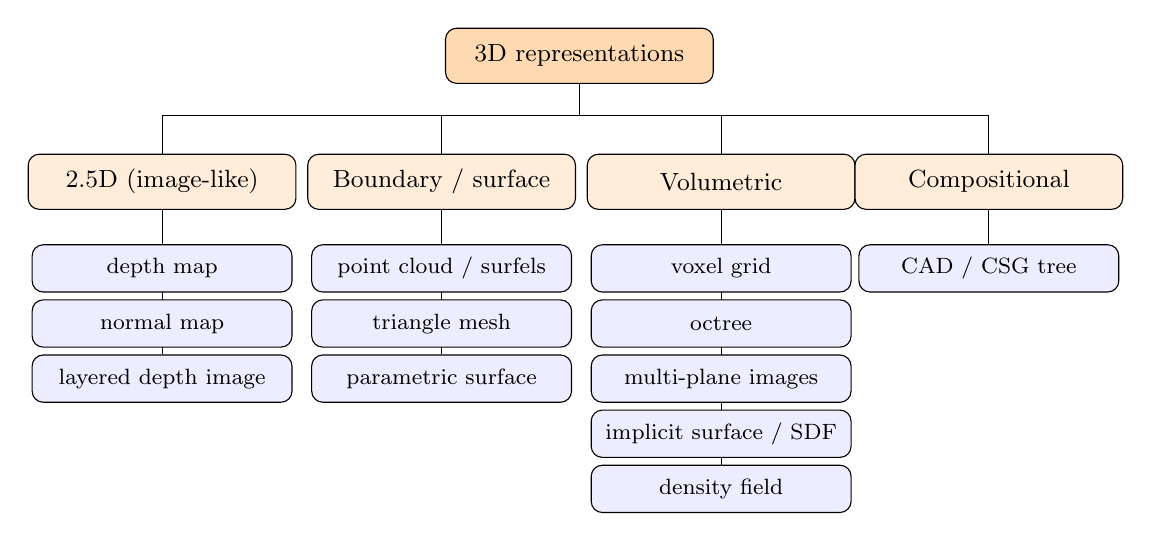
\begin{tikzpicture}[font=\small,
  lvl/.style={draw,rounded corners,fill=orange!15,minimum height=7mm,minimum width=3.4cm,align=center},
  ch/.style={draw,rounded corners,fill=blue!7,minimum height=6mm,minimum width=3.3cm,align=center,font=\footnotesize}]
\node[lvl,fill=orange!30] (root) at (0,0) {3D representations};
\node[lvl] (h) at (-5.3,-1.6) {2.5D (image-like)};
\node[lvl] (b) at (-1.75,-1.6) {Boundary / surface};
\node[lvl] (v) at (1.8,-1.6) {Volumetric};
\node[lvl] (c) at (5.2,-1.6) {Compositional};
\foreach \p in {h,b,v,c}{\draw (root.south) -- ++(0,-0.4) -| (\p.north);}
\node[ch] (h1) at (-5.3,-2.7) {depth map};
\node[ch] (h2) at (-5.3,-3.4) {normal map};
\node[ch] (h3) at (-5.3,-4.1) {layered depth image};
\node[ch] (b1) at (-1.75,-2.7) {point cloud / surfels};
\node[ch] (b2) at (-1.75,-3.4) {triangle mesh};
\node[ch] (b3) at (-1.75,-4.1) {parametric surface};
\node[ch] (v1) at (1.8,-2.7) {voxel grid};
\node[ch] (v2) at (1.8,-3.4) {octree};
\node[ch] (v3) at (1.8,-4.1) {multi-plane images};
\node[ch] (v4) at (1.8,-4.8) {implicit surface / SDF};
\node[ch] (v5) at (1.8,-5.5) {density field};
\node[ch] (c1) at (5.2,-2.7) {CAD / CSG tree};
\begin{scope}[on background layer]
\draw (h.south) -- (h3.north);
\draw (b.south) -- (b3.north);
\draw (v.south) -- (v5.north);
\draw (c.south) -- (c1.north);
\end{scope}
\end{tikzpicture}
\caption{A map of the representations met in the lecture (our grouping, following slides 43 and 63: points, meshes and parametric surfaces are \emph{boundary} representations; voxels and implicit fields are \emph{volumetric}).}
\end{figure}

% =====================================================================
\section{Notation \slides{slide 5}}
% =====================================================================

\begin{definition}[Notation]
A point in 3D space is written in inhomogeneous coordinates as
\[
\vx=\begin{pmatrix}x\\y\\z\end{pmatrix}\in\R^3 .
\]
A point on the image plane carries the subscript $s$: $\vx_s\in\R^2$. Discrete maps are \emph{indexed} rather than evaluated, and brackets denote indexing:
\[
D[\vx_s]\in\R^+ \quad(\text{depth}),\qquad N[\vx_s]\in\Sph^2 \quad(\text{unit normal}),\qquad V[i,j,k]\in[0,1]\quad(\text{occupancy}).
\]
\end{definition}

\begin{remark}
The subscript denotes the \emph{coordinate frame}, not the dimension of the space. Both $\vx$ and $\vx_s$ denote points.
\end{remark}

\begin{intuition}
Parentheses mean ``compute'' ($f(\vx)$ runs a formula or a network); brackets mean ``look up'' ($D[\vx_s]$ reads a pixel). The letter $s$ is a hint that $\vx_s$ lives on the \emph{s}creen; it is a name tag, not an exponent.
\end{intuition}

% =====================================================================
\section{Manifolds \slides{slide 6}}
% =====================================================================

\begin{definition}[Manifold]
An $n$-dimensional \emph{manifold} is a topological space that locally resembles Euclidean space: every point has a neighborhood homeomorphic to an open subset of $\R^n$; $n$ is its dimension.
\end{definition}

Lines and circles are $1$-manifolds. Two-dimensional manifolds are called \emph{surfaces}: the plane, the sphere, the torus. Each coloured piece of the shape on the slide is a \emph{chart}: it flattens a part of the shape onto $\R^n$.

\begin{figure}[ht]
\centering
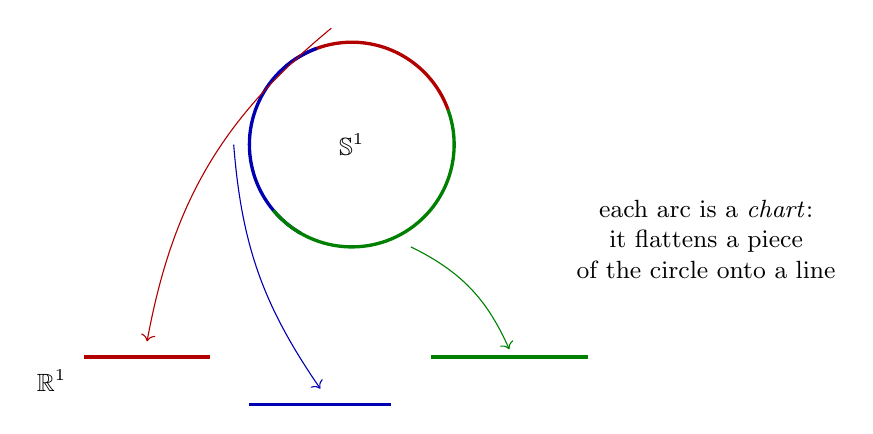
\begin{tikzpicture}[font=\small,scale=1]
\draw[gray!50] (0,0) circle (1.3);
\draw[very thick,red!70!black] (0,0)++(20:1.3) arc (20:130:1.3);
\draw[very thick,blue!70!black] (0,0)++(110:1.3) arc (110:240:1.3);
\draw[very thick,green!50!black] (0,0)++(220:1.3) arc (220:380:1.3);
\node at (0,0) {$\Sph^1$};
\begin{scope}[yshift=-3.3cm]
\draw[very thick,red!70!black] (-3.4,0.6) -- (-1.8,0.6);
\draw[very thick,blue!70!black] (-1.3,0) -- (0.5,0);
\draw[very thick,green!50!black] (1.0,0.6) -- (3.0,0.6);
\node[left] at (-3.5,0.3) {$\R^1$};
\end{scope}
\draw[->,red!70!black] (100:1.5) to[bend right=20] (-2.6,-2.5);
\draw[->,blue!70!black] (180:1.5) to[bend right=15] (-0.4,-3.1);
\draw[->,green!50!black] (300:1.5) to[bend left=20] (2.0,-2.6);
\node[align=center] at (4.5,-1.2) {each arc is a \emph{chart}:\\it flattens a piece\\of the circle onto a line};
\end{tikzpicture}
\caption{The circle is a $1$-manifold. Three overlapping charts, each a homeomorphism from an arc to an interval of $\R$, cover it. (Slide 6 shows the same idea for a circle and a sphere.)}
\end{figure}

\begin{intuition}
An ant walking on a sphere sees a flat plane around itself: that local flatness is what ``manifold'' means. The sphere as a whole is \emph{not} a plane, which is why one needs several overlapping charts (an atlas) to describe it, exactly as one needs several flat maps to cover the Earth without cutting it.
\end{intuition}

% =====================================================================
\section{Defining a Surface \slides{slide 7}}
% =====================================================================

\begin{definition}[Parametric and implicit forms]
A surface can be specified in two ways.
\begin{itemize}[nosep]
\item \textbf{Parametric form:} a function maps a 2D domain into space,
$f(\vu)=\vx\in\R^3,\ \vu\in\M$.
\item \textbf{Implicit form:} the surface is the zero level set of a scalar field, $\Surf=\{\vx\mid f(\vx)=0\}$.
\end{itemize}
In the parametric form the domain point $\vu$ is \emph{not} a point in space: it belongs to a 2D manifold $\M$, for instance the sphere $\Sph^2$.
\end{definition}

\begin{remark}
The symbol $f$ denotes both functions; the argument decides which is meant: $f(\vu)$ returns a surface point, $f(\vx)$ returns a scalar.
\end{remark}

\begin{intuition}
Parametric = ``a recipe that \emph{produces} points'' (feed in a domain point, get a 3D point out). Implicit = ``a rule that \emph{judges} points'' (feed in a 3D point, get a number whose sign says on which side of the surface it lies). Slide 48 will turn this into the mantra \emph{parametric generates, implicit tests}.
\end{intuition}

% =====================================================================
\section{Meanwhile in 3D-land\dots\ \slides{slides 8--9}}
% =====================================================================

``But what is the \emph{best} representation?'' The slide's answer: \emph{it depends}, on the task: acquisition vs editing vs animation vs prediction vs processing vs optimization, and more.

The goals of the lecture (slide 9):
\begin{itemize}[nosep]
\item understand representations \emph{computationally} (what do they look like in code?);
\item understand their limitations and benefits;
\item understand conversions across representations.
\end{itemize}

\begin{intuition}
There is no free lunch: a representation that makes one operation trivial tends to make another one painful. Reading each representation below, ask three questions: how do I \emph{store} it, what is \emph{easy} to do with it, what is \emph{hard}?
The lecture proceeds from representations tied to sensors (depth maps, point clouds), through surfaces (meshes, parametric surfaces), to volumes (voxels, implicit fields, density fields).
\end{intuition}

% =====================================================================
\section{Depth Maps \slides{slides 10--14}}
% =====================================================================

\subsection{Depth maps \slides{slides 10--12}}
Depth is a \emph{common modality across sensors} (structured-light and time-of-flight cameras such as the Kinect and industrial cameras shown on slide 10); depth is treated in detail in Lectures 04--05.

\begin{definition}[Depth map]
A depth map is an image $D[\vx_s]\in\R^+$ that records how far the scene point seen by each pixel $\vx_s$ is from the camera.
\end{definition}

Because it is just an image, \emph{standard image-processing tools can be used} on it (slide 12): filtering, resizing, convolutional networks.

\subsection{Depth Maps and Normal Maps \slides{slide 13}}
The same idea extends to other surface properties, e.g.\ surface normals:
\begin{definition}[Normal map]
$N[\vx_s]\in\Sph^2$ stores, for each pixel, the unit normal of the visible surface.
\end{definition}

\begin{figure}[H]
\centering
\includegraphics[width=0.75\textwidth]{depth_normal.png}
\caption{Depth and normal maps of a scene. The depth map is a grayscale image where brightness encodes distance; the normal map is a color image where RGB encodes the XYZ components of the unit normal.}
\end{figure}


\subsection{Depth Maps --- Representing the Visible \slides{slide 14}}
\begin{remark}
A depth map does not capture the \emph{full} 3D structure: it is a \emph{2.5D} representation, i.e.\ properties associated with image pixels. The slide asks: can we develop more \emph{complete} 3D representations?
\end{remark}

\begin{figure}[ht]
\centering
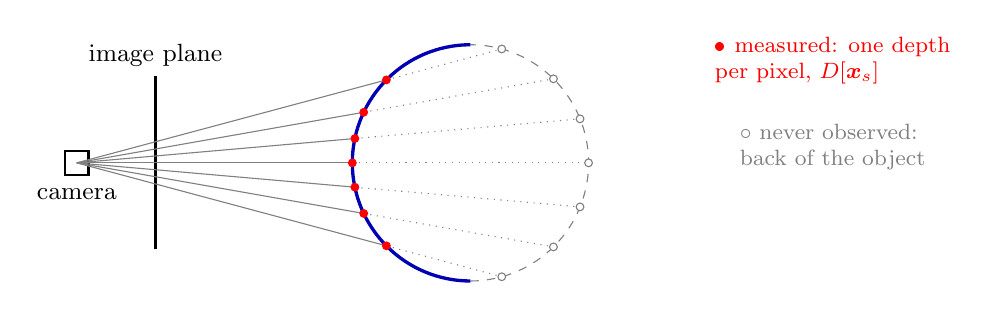
\begin{tikzpicture}[font=\small]
\draw[thick] (-0.15,-0.15) rectangle (0.15,0.15); \node[below] at (0,-0.2) {camera};
\draw[thick] (1,-1.1) -- (1,1.1); \node[above] at (1,1.1) {image plane};
\draw[dashed,gray] (5,0)++(-90:1.5) arc (-90:90:1.5);
\draw[very thick,blue!70!black] (5,0)++(90:1.5) arc (90:270:1.5);
\foreach \a in {-15,-10,-5,0,5,10,15}{
  \pgfmathsetmacro{\t}{5*cos(\a)-sqrt((5*cos(\a))^2-22.75)}
  \pgfmathsetmacro{\tb}{5*cos(\a)+sqrt((5*cos(\a))^2-22.75)}
  \draw[gray] (0,0) -- (\a:\t);
  \draw[dotted,gray] (\a:\t) -- (\a:\tb);
  \fill[red] (\a:\t) circle (1.6pt);
  \draw[gray,fill=white] (\a:\tb) circle (1.4pt);
}
\node[red,align=left,font=\footnotesize] at (9.6,1.3) {\textbullet\ measured: one depth\\per pixel, $D[\vx_s]$};
\node[gray,align=left,font=\footnotesize] at (9.6,0.2) {$\circ$ never observed:\\back of the object};
\end{tikzpicture}
\caption{Side view of a depth camera. Each pixel ray returns the \emph{first} surface hit (red); the far side of the object (dashed) and anything hidden behind the visible surface is absent from $D$.}
\end{figure}

\begin{intuition}
A depth map is like a relief map seen from one viewpoint: it tells the distance to whatever is \emph{in front}, and nothing about what is behind it. Two things follow. First, cheap and fast: it is an ordinary image. Second, incomplete: to model a whole object you need several views or a representation that lives in 3D itself, which motivates point clouds next.
\end{intuition}

% =====================================================================
\section{Point Clouds \slides{slides 15--21}}
% =====================================================================

\subsection{Point Clouds \slides{slides 15--18}}
\begin{figure}[H]
\centering
\includegraphics[width=0.75\textwidth]{pointcloud.png}
\caption{Some point clouds of scenes. Each point is a 3D position, and can be drawn as a small sphere.}
\end{figure}

Point clouds are often acquired in an image-like manner from sensors (LiDAR, depth cameras) but it can be useful to \emph{forget} this: point clouds from multiple views can be merged into a single point cloud, which helps unify approaches independently of the sensing modality.

\begin{definition}[Point cloud]
A point cloud is an \emph{unordered set} of points $\{\vx_1,\vx_2,\dots,\vx_N\}\subset\R^3$, usually stored as an $N\times 3$ array. Reordering the rows by any permutation $\sigma$ gives $\{\vx_{\sigma(1)},\dots,\vx_{\sigma(N)}\}$, the \emph{same} point cloud.
\end{definition}

Unlike an image, the row order carries no meaning, so processing or generation methods must be \emph{permutation invariant}; a fully connected layer applied to the flattened array does not work.

\begin{example}[Why a fully connected layer fails]
Let $X=\{\vx_1=(1,0,0),\,\vx_2=(0,1,0)\}$. Flattened, the two orderings give $(1,0,0,0,1,0)$ and $(0,1,0,1,0,0)$, two different vectors, so a generic linear layer returns two different outputs for one geometric object. A \emph{symmetric} operation such as taking the per-coordinate maximum over the points returns $(1,1,0)$ in both orders.
\end{example}

\begin{intuition}
Think of a bag of marbles: shaking it does not change what it contains. An operator must treat the input as a bag, not as a list. Symmetric functions (sum, mean, max over points) have this property, and network designs for point clouds are built from them.
\end{intuition}

\subsection{Oriented Point Clouds \slides{slide 19}}
\begin{definition}[Oriented point cloud, surfel]
An oriented point cloud stores a normal with each point: $\{(\vx_1,\vn_1),\dots,(\vx_N,\vn_N)\}$. Points can then be treated as small flat disks rather than tiny spheres, which helps rendering under lighting. When a radius is also stored the primitives are called \emph{surfels}.
\end{definition}

\begin{figure}[ht]
\centering
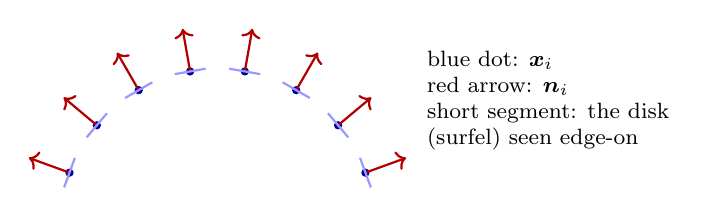
\begin{tikzpicture}[font=\small]
\foreach \a in {20,40,...,160}{
  \fill[blue!60!black] (\a:2) circle (1.5pt);
  \draw[->,red!70!black,thick] (\a:2) -- (\a:2.55);
  \draw[thick,blue!40] ($(\a:2)+(\a+90:0.2)$) -- ($(\a:2)+(\a-90:0.2)$);
}
\node[align=left,font=\footnotesize] at (4.2,1.6) {blue dot: $\vx_i$\\red arrow: $\vn_i$\\short segment: the disk\\(surfel) seen edge-on};
\end{tikzpicture}
\caption{An oriented point cloud sampled from a curve (2D cross-section): each sample carries a position and a normal, and can be drawn as a small disk perpendicular to the normal.}
\end{figure}

\begin{figure}[H]
\centering
\includegraphics[width=0.75\textwidth]{surfels.png}
\caption{A surfel-based reconstruction of a dinosaur. Each surfel is a small disk with a position, a normal and a radius.}
\end{figure}


\begin{intuition}
A bare point has no facing direction, so lighting is ambiguous. Attaching a normal turns each point into a tiny mirror; adding a radius makes the mirror cover a patch of surface, so neighbours overlap and the gaps between samples close up.
\end{intuition}

\subsection{No explicit connectivity \slides{slides 20--21}}
A point cloud has no explicit \emph{connectivity} information. Two point sets that look nearly identical may come from a closed circle and from a circle with a small gap. One can always sample more points to resolve the gap, but this is super inefficient; it is more efficient to add \emph{edges}, because connectivity does not scale like density (which grows with an area).

\begin{figure}[ht]
\centering
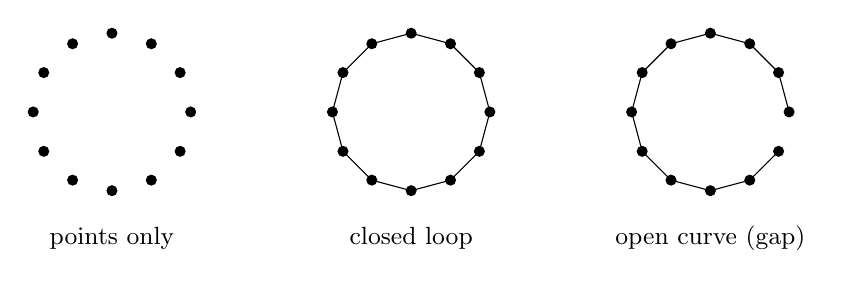
\begin{tikzpicture}[font=\small]
\foreach \i in {0,...,11}{\fill (30*\i:1) circle (2pt);}
\node at (0,-1.6) {points only};
\begin{scope}[xshift=3.8cm]
\foreach \i/\j in {0/1,1/2,2/3,3/4,4/5,5/6,6/7,7/8,8/9,9/10,10/11,11/0}{\draw (30*\i:1) -- (30*\j:1);}
\foreach \i in {0,...,11}{\fill (30*\i:1) circle (2pt);}
\node at (0,-1.6) {closed loop};
\end{scope}
\begin{scope}[xshift=7.6cm]
\foreach \i/\j in {0/1,1/2,2/3,3/4,4/5,5/6,6/7,7/8,8/9,9/10,10/11}{\draw (30*\i:1) -- (30*\j:1);}
\foreach \i in {0,...,11}{\fill (30*\i:1) circle (2pt);}
\node at (0,-1.6) {open curve (gap)};
\end{scope}
\end{tikzpicture}
\caption{The same 12 points support two different shapes: only the edges (connectivity) tell them apart.}
\end{figure}

\begin{example}[Density vs.\ connectivity]
To sample a unit sphere with spacing $h$ one needs roughly $4\pi/h^2$ points: about $1257$ for $h=0.1$ but about $5027$ for $h=0.05$. Halving the spacing multiplies the number of points by $4$, while adding one edge costs one pair of integers.
\end{example}

\begin{intuition}
Density is a \emph{2D} bill (points per unit area), connectivity is a \emph{1D} one (a few edges along features). To say ``these two neighbouring points belong to the same continuous piece'' it is far cheaper to draw a line than to fill the gap with hundreds of extra samples. This is exactly what meshes do.
\end{intuition}

% =====================================================================
\section{Meshes \slides{slides 22--34}}
% =====================================================================

\subsection{Meshes: vertices and faces \slides{slides 22--25}}
Meshes are \emph{piecewise linear approximations} of the underlying surface; more elements allow a better approximation (slide 22 shows a torus with increasing resolution).

\begin{figure}[H]
\centering
\includegraphics[width=0.75\textwidth]{mesh_torus.png}
\caption{A torus approximated by a mesh of increasing resolution and the difference between a mesh and a pointcloud of a rabbit. The mesh is a
 piecewise linear approximation of the underlying surface.}
\end{figure}
\begin{definition}[Mesh]
A mesh is a pair $(V,F)$: $V$ is an $N\times 3$ array of vertex positions (the \emph{geometry}) and $F$ is a list of $M$ faces (the \emph{topology}), each face being a list of indices of the vertices that make it up. Consecutive indices in a face are joined by an edge, so \emph{ordering matters} in face indices.
\end{definition}

\begin{figure}[ht]
\centering
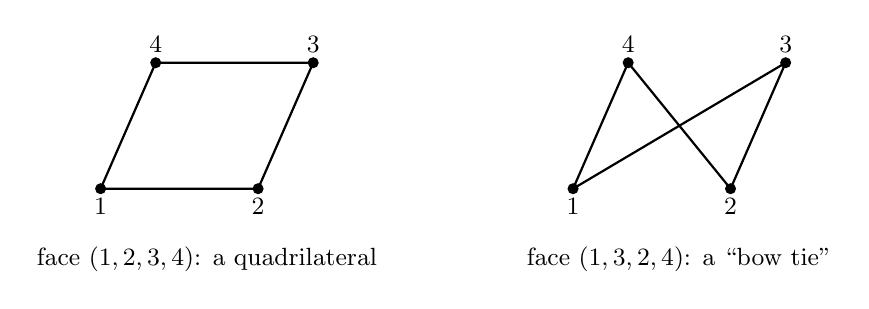
\begin{tikzpicture}[font=\small]
\begin{scope}
\draw[thick] (0,0)--(2,0)--(2.7,1.6)--(0.7,1.6)--cycle;
\foreach \p/\l/\pos in {(0,0)/1/below,(2,0)/2/below,(2.7,1.6)/3/above,(0.7,1.6)/4/above}{\fill \p circle (2pt); \node[\pos] at \p {\l};}
\node at (1.35,-0.9) {face $(1,2,3,4)$: a quadrilateral};
\end{scope}
\begin{scope}[xshift=6cm]
\draw[thick] (0,0)--(2.7,1.6)--(2,0)--(0.7,1.6)--cycle;
\foreach \p/\l/\pos in {(0,0)/1/below,(2,0)/2/below,(2.7,1.6)/3/above,(0.7,1.6)/4/above}{\fill \p circle (2pt); \node[\pos] at \p {\l};}
\node at (1.35,-0.9) {face $(1,3,2,4)$: a ``bow tie''};
\end{scope}
\end{tikzpicture}
\caption{Same four vertices, two index orders, two different shapes: consecutive indices are connected by an edge.}
\end{figure}

Arbitrary polygons can also be \emph{non-planar} (four points in 3D need not lie in a plane), so one restricts to triangles: three points not on a line always define a plane.

\begin{figure}[ht]
\centering
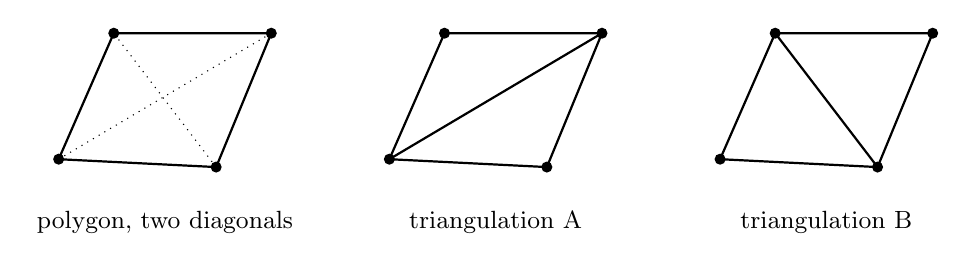
\begin{tikzpicture}[font=\small]
\foreach \dx/\kind in {0/0,4.2/1,8.4/2}{
 \begin{scope}[xshift=\dx cm]
 \draw[thick] (0,0)--(2,-0.1)--(2.7,1.6)--(0.7,1.6)--cycle;
 \ifnum\kind=0 \draw[dotted] (0,0)--(2.7,1.6); \draw[dotted] (2,-0.1)--(0.7,1.6); \fi
 \ifnum\kind=1 \draw[thick] (0,0)--(2.7,1.6); \fi
 \ifnum\kind=2 \draw[thick] (2,-0.1)--(0.7,1.6); \fi
 \foreach \p in {(0,0),(2,-0.1),(2.7,1.6),(0.7,1.6)}{\fill \p circle (2pt);}
 \end{scope}
}
\node at (1.35,-0.8) {polygon, two diagonals};
\node at (5.55,-0.8) {triangulation A};
\node at (9.75,-0.8) {triangulation B};
\end{tikzpicture}
\caption{A quad can be split into triangles in two ways. If the four points are not coplanar, A and B are two genuinely different surfaces, while each triangle on its own is always flat.}
\end{figure}

\subsection{Triangular Meshes \slides{slides 26--31}}
\begin{definition}[Triangular mesh]
A triangular mesh is a mesh whose faces are all triangles: $V\in\R^{N\times 3}$ and $F\in\{0,\dots,N-1\}^{M\times 3}$, each row of $F$ listing the indices of the \emph{three} vertices of a face.
\end{definition}

\begin{example}[A tetrahedron in code]
\begin{lstlisting}
V = np.array([[0,0,0],[1,0,0],[0,1,0],[0,0,1]], dtype=float)   # 4 x 3
F = np.array([[0,2,1],[0,1,3],[0,3,2],[1,2,3]])                # 4 x 3, ints
\end{lstlisting}
Here $N=4$ vertices, $M=4$ faces and $E=6$ edges.
\end{example}

\paragraph{A sanity check on sizes.}
\begin{proposition}[Face count of a closed genus-0 triangle mesh]\label{prop:euler}
Let a closed, sphere-like (genus~0) triangular mesh have $V$ vertices, $E$ edges and $F$ faces. Every face has $3$ edges and every edge is shared by $2$ faces, so $E=3F/2$. With Euler's formula $V-E+F=2$ this gives
\[
F=2V-4 .
\]
\end{proposition}
\begin{proof}
Substitute $E=3F/2$ into $V-E+F=2$: $V-\tfrac32F+F=2$, i.e.\ $V-\tfrac12F=2$, hence $F=2V-4$.
\end{proof}

\begin{intuition}
You get about \emph{twice as many triangles as vertices}. Checks: tetrahedron $V=4\Rightarrow F=4$ \checkmark; octahedron $V=6\Rightarrow F=8$ \checkmark; a scan with $V=10{,}000$ vertices has $F=19{,}996$ faces and $E=3F/2=29{,}994$ edges. Useful to guess memory footprints or to spot a broken mesh.
\end{intuition}

\paragraph{Orientation.} For a triangle, \emph{any order gives the same triangle}, but the order determines which side is ``front''. The normal is $\vn=(\vb-\va)\times(\vc-\va)$.

\begin{proposition}[Orientation and index order]\label{prop:orient}
A cyclic shift $(a,b,c)\to(b,c,a)$ leaves $\vn$ unchanged; swapping two indices, e.g.\ $(a,b,c)\to(c,b,a)$, flips its sign.
\end{proposition}
\begin{proof}
Expanding, $(\vb-\va)\times(\vc-\va)=\vb\times\vc-\vb\times\va-\va\times\vc+\va\times\va=\va\times\vb+\vb\times\vc+\vc\times\va$. This expression is unchanged by cyclic relabelling $\va\to\vb\to\vc\to\va$ and changes sign under the swap of any two symbols, since $\times$ is antisymmetric.
\end{proof}

\begin{figure}[ht]
\centering
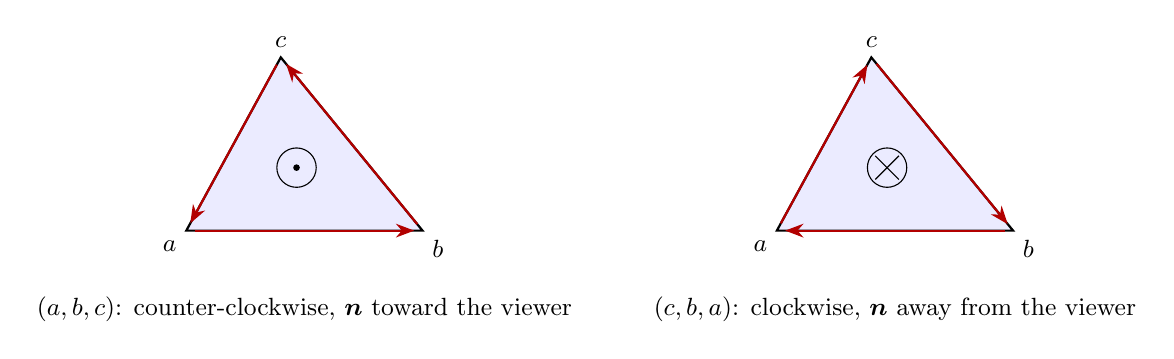
\begin{tikzpicture}[font=\small,>=Stealth]
\begin{scope}
\coordinate (a) at (0,0); \coordinate (b) at (3,0); \coordinate (c) at (1.2,2.2);
\draw[thick,fill=blue!8] (a)--(b)--(c)--cycle;
\draw[->,thick,red!70!black,shorten >=3pt,shorten <=3pt] (a)--(b);
\draw[->,thick,red!70!black,shorten >=3pt,shorten <=3pt] (b)--(c);
\draw[->,thick,red!70!black,shorten >=3pt,shorten <=3pt] (c)--(a);
\node[below left] at (a) {$a$}; \node[below right] at (b) {$b$}; \node[above] at (c) {$c$};
\node[draw,circle,inner sep=0pt,minimum size=5mm] at (1.4,0.8) {}; \fill (1.4,0.8) circle (1.2pt);
\node at (1.5,-1) {$(a,b,c)$: counter-clockwise, $\vn$ toward the viewer};
\end{scope}
\begin{scope}[xshift=7.5cm]
\coordinate (a) at (0,0); \coordinate (b) at (3,0); \coordinate (c) at (1.2,2.2);
\draw[thick,fill=blue!8] (a)--(b)--(c)--cycle;
\draw[->,thick,red!70!black,shorten >=3pt,shorten <=3pt] (c)--(b);
\draw[->,thick,red!70!black,shorten >=3pt,shorten <=3pt] (b)--(a);
\draw[->,thick,red!70!black,shorten >=3pt,shorten <=3pt] (a)--(c);
\node[below left] at (a) {$a$}; \node[below right] at (b) {$b$}; \node[above] at (c) {$c$};
\node[draw,circle,inner sep=0pt,minimum size=5mm] at (1.4,0.8) {}; 
\draw (1.25,0.65)--(1.55,0.95); \draw (1.25,0.95)--(1.55,0.65);
\node at (1.5,-1) {$(c,b,a)$: clockwise, $\vn$ away from the viewer};
\end{scope}
\end{tikzpicture}
\caption{Index order defines the winding direction and hence the side the normal points to. Swapping two indices reverses it.}
\end{figure}

\begin{example}[Checking the tetrahedron]
For face $(0,2,1)$ of the example above, $\va=(0,0,0)$, $\vb=(0,1,0)$, $\vc=(1,0,0)$: $\vn=(0,1,0)\times(1,0,0)=(0,0,-1)$, pointing down, i.e.\ \emph{outward} for the face lying in $z=0$ (the tetrahedron sits above it). Face $(1,2,3)$ gives $(-1,1,0)\times(-1,0,1)=(1,1,1)$, also outward. All four faces are consistently oriented.
\end{example}

\begin{intuition}
The ``classic bug'': if some faces are listed clockwise and others counter-clockwise, the renderer treats some triangles as back-facing and they render black or vanish. Rule of thumb: use one winding convention for the whole mesh and check with $\vn$ pointing away from the interior.
\end{intuition}

\paragraph{Manifold problems.}
Even with triangles one can still get \emph{non-manifold} meshes. The slides identify two cases: an edge shared by more than two faces (so restrict each edge to at most two faces; one can often get away without enforcing this) and a \emph{disconnected surface around a vertex}, which is critical for mesh-processing applications and less so for rendering.

\begin{figure}[ht]
\centering
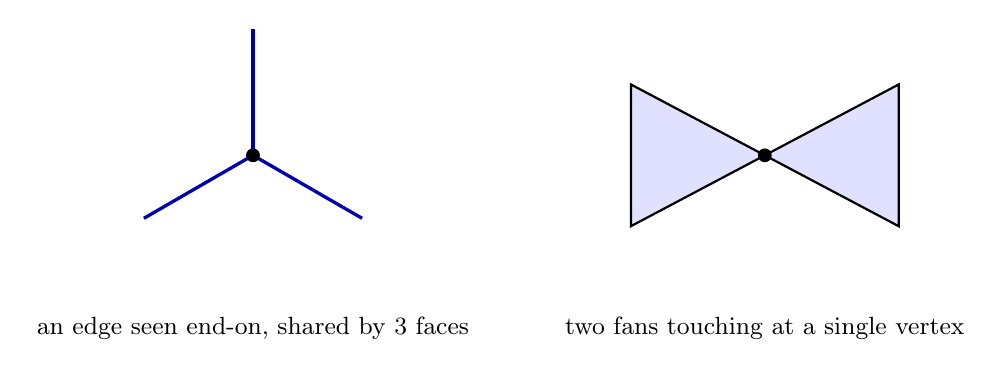
\begin{tikzpicture}[font=\small]
\begin{scope}
\foreach \a in {90,210,330}{\draw[very thick,blue!70!black] (0,0) -- (\a:1.6);}
\fill (0,0) circle (2.5pt);
\node at (0,-2.2) {an edge seen end-on, shared by 3 faces};
\end{scope}
\begin{scope}[xshift=6.5cm]
\draw[thick,fill=blue!12] (0,0) -- (-1.7,0.9) -- (-1.7,-0.9) -- cycle;
\draw[thick,fill=blue!12] (0,0) -- (1.7,0.9) -- (1.7,-0.9) -- cycle;
\fill (0,0) circle (2.5pt);
\node at (0,-2.2) {two fans touching at a single vertex};
\end{scope}
\end{tikzpicture}
\caption{Two kinds of non-manifold configuration.}
\end{figure}

\paragraph{Ray--triangle intersection and texturing.}
\begin{proposition}[Barycentric form and the ray--triangle solve]\label{prop:ray}
Any point of the triangle with vertices $\va,\vb,\vc$ is $\alpha\va+\beta\vb+\gamma\vc$ with $\alpha+\beta+\gamma=1$ and all three weights $\ge 0$. Setting this equal to the ray $\vo+t\vd$ gives $3$ linear equations in the $3$ unknowns $(t,\beta,\gamma)$, i.e.\ a $3\times 3$ solve per triangle:
\[
\beta(\vb-\va)+\gamma(\vc-\va)-t\,\vd=\vo-\va ,\qquad \alpha=1-\beta-\gamma .
\]
The ray hits the triangle iff $\beta\ge0$, $\gamma\ge0$, $\beta+\gamma\le 1$ (and $t>0$).
\end{proposition}
\begin{proof}
Substitute $\alpha=1-\beta-\gamma$ in $\alpha\va+\beta\vb+\gamma\vc=\vo+t\vd$ and collect terms.
\end{proof}

\begin{example}
Triangle $\va=(0,0,0)$, $\vb=(1,0,0)$, $\vc=(0,1,0)$; ray $\vo=(0.25,0.25,1)$, $\vd=(0,0,-1)$. The system reads $\beta(1,0,0)+\gamma(0,1,0)-t(0,0,-1)=(0.25,0.25,1)$, so $\beta=\gamma=0.25$, $t=1$, $\alpha=0.5$. All weights are $\ge0$: hit at $\vo+\vd=(0.25,0.25,0)$.
\end{example}

Texturing is easy: each vertex also stores a coordinate into a 2D image, and inside a triangle the same weights interpolate those coordinates.

\begin{figure}[ht]
\centering
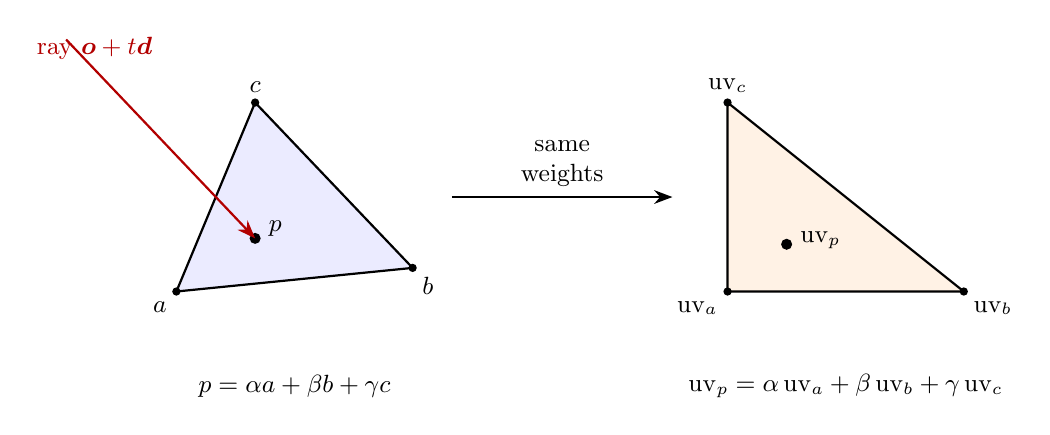
\begin{tikzpicture}[font=\small,>=Stealth]
\coordinate (a) at (0,0); \coordinate (b) at (3,0.3); \coordinate (c) at (1,2.4);
\coordinate (p) at (1,0.675);
\draw[thick,fill=blue!8] (a)--(b)--(c)--cycle;
\fill (p) circle (2pt);
\foreach \v/\l/\pos in {a/a/below left,b/b/below right,c/c/above}{\fill (\v) circle (1.5pt); \node[\pos] at (\v) {$\l$};}
\node[right] at (1.05,0.8) {$p$};
\draw[->,thick,red!70!black] (-1.4,3.2) -- (p) node[pos=0.15,above] {ray $\vo+t\vd$};
\node[align=center] at (1.5,-1.2) {$p=\alpha a+\beta b+\gamma c$};
\begin{scope}[xshift=7cm]
\coordinate (a2) at (0,0); \coordinate (b2) at (3,0); \coordinate (c2) at (0,2.4);
\coordinate (p2) at (0.75,0.6);
\draw[thick,fill=orange!10] (a2)--(b2)--(c2)--cycle;
\fill (p2) circle (2pt);
\foreach \v/\l/\pos in {a2/{a}/below left,b2/{b}/below right,c2/{c}/above}{\fill (\v) circle (1.5pt); \node[\pos] at (\v) {$\mathrm{uv}_\l$};}
\node[right] at (0.8,0.65) {$\mathrm{uv}_p$};
\node[align=center] at (1.5,-1.2) {$\mathrm{uv}_p=\alpha\,\mathrm{uv}_a+\beta\,\mathrm{uv}_b+\gamma\,\mathrm{uv}_c$};
\end{scope}
\draw[->,thick] (3.5,1.2) -- (6.3,1.2) node[midway,above,align=center] {same\\weights};
\end{tikzpicture}
\caption{Left: the hit point in barycentric coordinates $(\alpha,\beta,\gamma)=(0.5,0.25,0.25)$. Right: the same weights interpolate the 2D texture coordinates stored at the vertices.}
\end{figure}

\begin{intuition}
Barycentric weights are ``how much of each corner'' a point is made of; a point near $a$ has $\alpha$ close to $1$. Intersecting a ray with a triangle is therefore a tiny linear-algebra problem, which is why GPUs can do billions of them, and the \emph{same} weights carry any per-vertex quantity (texture coordinates, colours, normals) to the interior.
\end{intuition}

\subsection{Triangular Meshes --- Geometry vs Connectivity \slides{slides 32--34}}
The two arrays of a mesh behave very differently:
$V$ is \texttt{float}, differentiable, and gradient descent (GD) is happy; $F$ is \texttt{int}, discrete, and GD is not happy. Modifying vertex positions can edit the shape; other changes are non-trivial (i.e.\ changing $F$).

\begin{figure}[H]
\centering
\includegraphics[width=0.75\textwidth]{geometry_connectivity.png}
\caption{Editing the geometry $V$ is easy, editing the connectivity $F$ is hard.}
\end{figure}

\begin{figure}[ht]
\centering
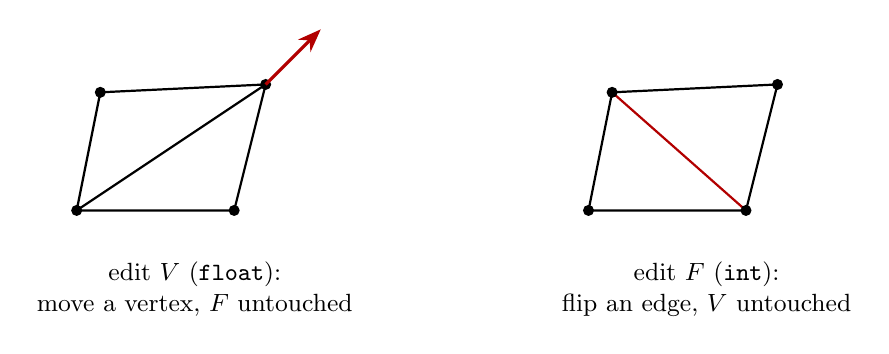
\begin{tikzpicture}[font=\small,>=Stealth]
\begin{scope}
\draw[thick] (0,0)--(2,0)--(2.4,1.6)--(0.3,1.5)--cycle; \draw[thick] (0,0)--(2.4,1.6);
\foreach \p in {(0,0),(2,0),(2.4,1.6),(0.3,1.5)}{\fill \p circle (2pt);}
\draw[->,red!70!black,very thick] (2.4,1.6) -- (3.1,2.3);
\node[align=center] at (1.5,-1) {edit $V$ (\texttt{float}):\\move a vertex, $F$ untouched};
\end{scope}
\begin{scope}[xshift=6.5cm]
\draw[thick] (0,0)--(2,0)--(2.4,1.6)--(0.3,1.5)--cycle; \draw[thick,red!70!black] (2,0)--(0.3,1.5);
\foreach \p in {(0,0),(2,0),(2.4,1.6),(0.3,1.5)}{\fill \p circle (2pt);}
\node[align=center] at (1.5,-1) {edit $F$ (\texttt{int}):\\flip an edge, $V$ untouched};
\end{scope}
\end{tikzpicture}
\caption{Geometry edits are small continuous changes of real numbers; connectivity edits are combinatorial jumps.}
\end{figure}

\subsubsection*{Same counts, different meshes \slides{slide 33}}
Going from one mesh to another is non-trivial even when both have $6$ vertices and $8$ faces (the octahedron is one such mesh). It is even more challenging if the topology changes, e.g.\ torus to sphere. In general, designing methods that can predict \emph{arbitrary} connectivity is challenging (e.g.\ image to mesh).
\begin{figure}[H]
\centering
\includegraphics[width=0.75\textwidth]{mesh_edit.png}
\caption{Two meshes with the same number of vertices and faces, but different connectivity.}
\end{figure}
\subsubsection*{Continuous deformation \slides{slide 34}}
The first change (same counts, different connectivity) is possible under continuous deformation of the shape; the torus-to-sphere change is impossible under continuous deformation (a hole cannot be closed without tearing). Yet \emph{both} edits require similar operations for meshes: a new $F$ and an updated $V$. The slide asks: is there an alternate representation where the former (the continuous one) is easier?

\begin{intuition}
A mesh mixes a smooth part ($V$) with a rigid combinatorial part ($F$). Even a tiny, continuous change of the shape may demand a jump in $F$, and a network cannot easily output ``an integer array of unknown length''. The question hanging in the air motivates representations where shape changes are always changes of continuous numbers: parametric and, above all, implicit ones.
\end{intuition}

% =====================================================================
\section{Parametric Surfaces \slides{slides 35--41}}
% =====================================================================

\subsection{Parametric surfaces in 2D \slides{slide 35}}
The domain is a circle $\Sph^1$; think of it as an angle $\theta$. A function $f(\vu)=\vx\in\R^2,\ \vu\in\Sph^1$ sends each angle to a point of a curve: $f_1$ to a pentagon, $f_2$ to a square.

\begin{figure}[ht]
\centering
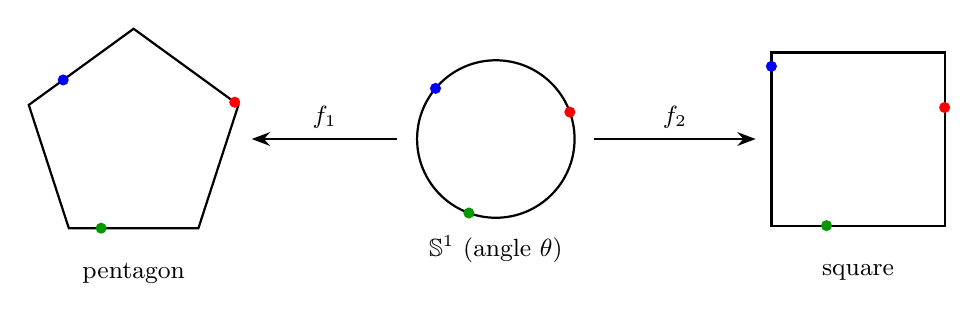
\begin{tikzpicture}[font=\small,>=Stealth]
\draw[thick] (0,0) circle (1);
\foreach \th/\col in {20/red,140/blue,250/green!60!black}{\fill[\col] (\th:1) circle (2pt);}
\node at (0,-1.4) {$\Sph^1$ (angle $\theta$)};
\begin{scope}[xshift=-4.6cm]
\draw[thick] (90:1.4)--(162:1.4)--(234:1.4)--(306:1.4)--(18:1.4)--cycle;
\foreach \th/\col in {20/red,140/blue,250/green!60!black}{
  \pgfmathsetmacro{\ph}{72*round((\th-54)/72)+54}
  \pgfmathsetmacro{\rr}{1.4*cos(36)/cos(\th-\ph)}
  \fill[\col] (\th:\rr) circle (2pt);}
\node at (0,-1.7) {pentagon};
\end{scope}
\begin{scope}[xshift=4.6cm]
\draw[thick] (-1.1,-1.1) rectangle (1.1,1.1);
\foreach \th/\col in {20/red,140/blue,250/green!60!black}{
  \pgfmathsetmacro{\ph}{90*round(\th/90)}
  \pgfmathsetmacro{\rr}{1.1/cos(\th-\ph)}
  \fill[\col] (\th:\rr) circle (2pt);}
\node at (0,-1.7) {square};
\end{scope}
\draw[->,thick] (-1.25,0) -- (-3.1,0) node[midway,above] {$f_1$};
\draw[->,thick] (1.25,0) -- (3.3,0) node[midway,above] {$f_2$};
\end{tikzpicture}
\caption{Two different maps $f_1,f_2$ from the same circle domain. Same colour = same domain point $\theta$.}
\end{figure}

\subsection{Parametric surfaces \slides{slides 36--40}}
\begin{definition}[Parametric surface]
A continuous function $f:\M\to\R^3$, $f(\vu)=\vx$, over a 2D manifold $\M$ parametrizes a surface. The \emph{connectivity/topology} is constrained to be the same as $\M$. This disentangles discretization (vertices/faces) from shape representation. In code:
\begin{lstlisting}
def f(u):
    '''Input:  u: N-dimensional vector from a 2D manifold
       Output: x: 3D point'''
\end{lstlisting}
$f$ can be a fixed analytic function, a parametrized family, or even a neural network $f_\theta:\Sph^2\to\R^3$.
\end{definition}

\begin{figure}[ht]
\centering
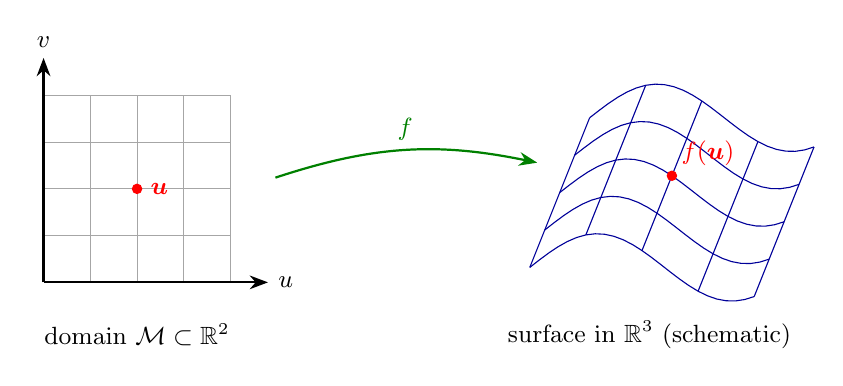
\begin{tikzpicture}[font=\small,>=Stealth,scale=0.95]
\begin{scope}
\foreach \u in {0,0.25,0.5,0.75,1}{\draw[gray!70] (2.5*\u,0)--(2.5*\u,2.5); \draw[gray!70] (0,2.5*\u)--(2.5,2.5*\u);}
\draw[->,thick] (0,0)--(3,0) node[right] {$u$}; \draw[->,thick] (0,0)--(0,3) node[above] {$v$};
\fill[red] (1.25,1.25) circle (2pt); \node[right,red] at (1.3,1.25) {$\vu$};
\node at (1.25,-0.7) {domain $\M\subset\R^2$};
\end{scope}
\begin{scope}[xshift=6.5cm,yshift=0.2cm]
\foreach \u in {0,0.25,0.5,0.75,1}{\draw[blue!60!black] plot[domain=0:1,samples=25,variable=\t] ({3*\u+0.8*\t},{2*\t+0.45*sin(300*\u)});}
\foreach \v in {0,0.25,0.5,0.75,1}{\draw[blue!60!black] plot[domain=0:1,samples=25,variable=\t] ({3*\t+0.8*\v},{2*\v+0.45*sin(300*\t)});}
\fill[red] (1.9,1.225) circle (2pt); \node[above right,red] at (1.9,1.225) {$f(\vu)$};
\node at (1.6,-0.9) {surface in $\R^3$ (schematic)};
\end{scope}
\draw[->,thick,green!50!black] (3.1,1.4) to[bend left=15] node[above] {$f$} (6.6,1.6);
\end{tikzpicture}
\includegraphics[width=0.75\textwidth]{parametric_surface.png}
\caption{A parametrization warps a flat domain into a surface: grid lines of $(u,v)$ become curves on the surface, and neighbouring parameters stay neighbouring.}
\end{figure}

\begin{example}[Analytic examples]
The saddle $f((u,v))=(u,\,v,\,v^2-u^2)$; and the trefoil-knot tube of slide 38:
\begin{lstlisting}
def trefoil(u, v):
    # r is just a float scale factor
    x = r * np.sin(3*u) / (2 + np.cos(v))
    y = r * (np.sin(u) + 2*np.sin(2*u)) / (2 + np.cos(v + np.pi*2/3))
    z = r/2 * (np.cos(u) - 2*np.cos(2*u)) * (2 + np.cos(v)) * (2 + np.cos(v + np.pi*2/3)) / 4
\end{lstlisting}
\end{example}

\begin{definition}[B\'ezier surface]
With $(N+1)(M+1)$ control points $\vk_{i,j}\in\R^3$,
\[
f((u,v))=\sum_{i=0}^{N}\sum_{j=0}^{M}B_i^N(u)\,B_j^M(v)\,\vk_{i,j},\qquad B_i^N(u)=\binom{N}{i}u^i(1-u)^{N-i}.
\]
Here $N$ and $M$ are polynomial \emph{degrees}, not counts. The control points determine a smooth surface in 3D; B\'ezier patches are commonly used for designing meshes.
\end{definition}
\begin{figure}[H]
\centering
\includegraphics[width=0.75\textwidth]{bezier_surface.png}
\caption{A B\'ezier surface}
\end{figure}

\begin{example}[The bilinear patch, $N=M=1$]
$B_0^1(u)=1-u$, $B_1^1(u)=u$, so $f=(1-u)(1-v)\vk_{00}+(1-u)v\,\vk_{01}+u(1-v)\vk_{10}+uv\,\vk_{11}$. With $\vk_{00}=(0,0,0)$, $\vk_{10}=(1,0,0)$, $\vk_{01}=(0,1,0)$, $\vk_{11}=(1,1,1)$: $f(0.5,0.5)=\tfrac14\big[(1,0,0)+(0,1,0)+(1,1,1)\big]=(0.5,0.5,0.25)$.
\end{example}

\begin{intuition}
Control points act like a coarse cage of pins: move a pin and the smooth sheet follows. The surface is a weighted average of the pins, with weights (Bernstein polynomials) that sum to one, so it stays inside the convex hull of the cage. That is why the same $(N+1)(M+1)$ numbers describe an entire smooth surface no matter how finely you later sample it.
\end{intuition}

\subsection{Parametric Surfaces --- Pros and Cons \slides{slide 41}}
\begin{itemize}[nosep]
\item \textbf{Sampling is easy:} pick $\vu$, evaluate $f$.
\item \textbf{Computation in the domain:} neighbours, texture coordinates and so on are just nearby $\vu$ values.
\item \textbf{``Is $\vq$ inside?'' is hard:} you would have to search for the $\vu$ whose $f(\vu)$ is closest to $\vq$, an optimization problem.
\item \textbf{Rendering is hard:} a ray hits the surface where $\vo+t\vd=f(\vu)$, a nonlinear system in $(t,\vu)$. In practice you convert to a mesh first.
\end{itemize}

\begin{intuition}
Generating is a \emph{forward} computation (plug in, read off); testing or intersecting needs the \emph{inverse} of $f$, which is generally not available in closed form. The price of the parametrization is also its topology: the surface has whatever topology $\M$ has (a sphere domain can only give sphere-like shapes).
\end{intuition}

% =====================================================================
\section{Surface Representations \slides{slide 42}}
% =====================================================================

Points, meshes and parametric surfaces all describe the ``skin'' of an object, and none of them can turn a torus into a sphere continuously. So what can we do?

\begin{intuition}
All three fix the topology in their data (the connectivity $F$, the domain $\M$, or the absence of connectivity). To let shapes change topology smoothly, one needs a representation that assigns a value to \emph{every point of space} rather than tracking the skin.
\end{intuition}

% =====================================================================
\section{Volume Representations \slides{slides 43--46}}
% =====================================================================

Volume representations give a value to every point in space.

\subsection{Voxelized 3D \slides{slides 44--46}}
\begin{definition}[Voxel grid]
A voxel grid is a discretized representation of the space demarcated via cuboid endpoints $(x_{\min},y_{\min},z_{\min})$ and $(x_{\max},y_{\max},z_{\max})$: a $W\times H\times D$ array $V[i,j,k]\in[0,1]$ storing the occupancy (or probability of occupancy) of each cell.
\end{definition}

\begin{figure}[H]
\centering
\includegraphics[width=0.75\textwidth]{voxel_grid.png}
\caption{A $4\times4\times4$ voxel grid inside a cuboid; shaded cells are occupied.}
\end{figure}

\textbf{Coding tip:} disentangle \emph{grid coordinates} from the \emph{spatial extent in the world}. One common convention: cell size $h=(x_{\max}-x_{\min})/W$ along $x$, and cell $i$ has its centre at $x_{\min}+(i+\tfrac12)h$; the same for $y,z$. For $x_{\min}=-1.5$, $x_{\max}=1.5$, $W=128$: $h\approx0.0234$, and the point $x=0.3$ falls in cell $i=\lfloor(0.3+1.5)/h\rfloor=76$.

Because the representation is ``image-like'', \emph{convolutions} can be used for processing and generation. It is a generic way to represent shapes \emph{across topologies}: the sphere, the torus and the cow of slide 45 all use the same array shape, and topology is just which cells are switched on. A fixed-size output is exactly what networks like.

\subsubsection*{Resolution is expensive \slides{slide 46}}
It is computationally challenging to scale resolution ($32^3,64^3,128^3,256^3$ on the slide). Worse, the surface passes through only about $n^2$ of the $n^3$ cells, so almost all the memory describes empty space or solid interior.

\begin{figure}[H]
\centering
\includegraphics[width=0.75\textwidth]{voxel_grid_resolution.png}
\caption{A rappresentation of how resolution affects surface detail. The surface passes through only about $n^2$ of the $n^3$ cells, so almost all the memory describes empty space or solid interior.}
\end{figure}

\begin{example}[Memory of a voxel grid]
\begin{center}
\begin{tabular}{rrrr}
\toprule
$n$ & cells $n^3$ & surface cells $\approx n^2$ & fraction $\approx 1/n$ \\
\midrule
32 & 32\,768 & 1\,024 & 3\% \\
64 & 262\,144 & 4\,096 & 1.6\% \\
128 & 2\,097\,152 & 16\,384 & 0.8\% \\
256 & 16\,777\,216 & 65\,536 & 0.4\% \\
\bottomrule
\end{tabular}
\end{center}
At one byte per cell, $256^3$ is 16\,MB (64\,MB with 32-bit floats) for a single object.
\end{example}

\begin{figure}[ht]
\centering
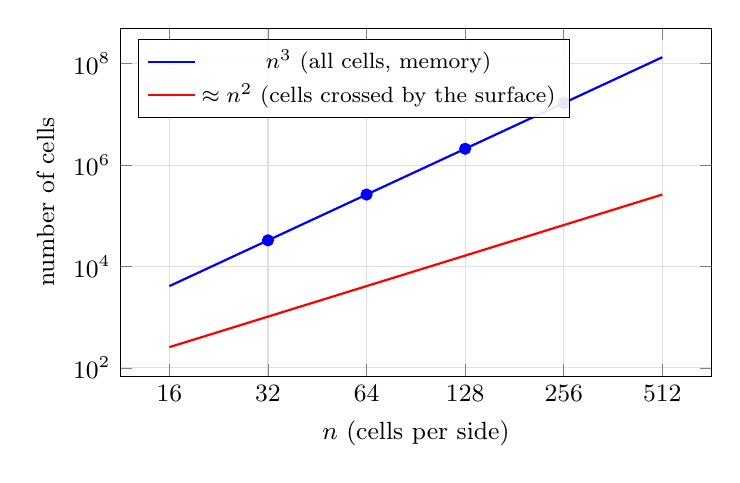
\begin{tikzpicture}
\begin{axis}[width=0.75\linewidth,height=6cm,xmode=log,ymode=log,xlabel={$n$ (cells per side)},ylabel={number of cells},
 xtick={16,32,64,128,256,512},xticklabels={16,32,64,128,256,512},grid=both,legend pos=north west,legend style={font=\footnotesize,fill=white,fill opacity=0.9,text opacity=1,draw opacity=1}]
\addplot[blue,thick,domain=16:512,samples=2] {x^3}; \addlegendentry{$n^3$ (all cells, memory)}
\addplot[red,thick,domain=16:512,samples=2] {x^2}; \addlegendentry{$\approx n^2$ (cells crossed by the surface)}
\addplot[only marks,mark=*,blue] coordinates {(32,32768)(64,262144)(128,2097152)(256,16777216)};
\end{axis}
\end{tikzpicture}
\caption{Doubling the resolution multiplies memory by 8 but the useful (surface) part only by 4.}
\end{figure}

\begin{intuition}
A voxel grid is a bookkeeping device: it pays the same for air as for the object. Doubling the resolution costs $8\times$ more memory but only $4\times$ more surface. The benefit is simplicity: any topology, fixed size, convolutions apply. The cost is that fine detail is very expensive, which motivates adaptive versions (octrees, slide 68) and continuous fields (next section).
\end{intuition}

% =====================================================================
\section{Implicit Surfaces \slides{slides 47--62}}
% =====================================================================

\subsection{Implicit surfaces \slides{slide 47}}
\begin{definition}[Implicit surface]
A surface is the \emph{zero level set} of a scalar field $f:\R^3\to\R$:
\[
\Surf=\{\vx\in\R^3\mid f(\vx)=0\}.
\]
The sign tells the side: $f(\vx)<0$ inside, $f(\vx)>0$ outside (one convention, used for the rest of the lecture).
\end{definition}

\subsection{Generate vs Test \slides{slide 48}}
The unit circle, written both ways:
\begin{center}
\begin{tabular}{L{3.2cm}L{5.4cm}L{5.4cm}}
\toprule
 & \textbf{Parametric} & \textbf{Implicit}\\
\midrule
Definition & $g(u)=(\cos u,\sin u)$, $u\in[0,2\pi)$ & $f(x,y)=x^2+y^2-1$\\
Give me 100 points on it & easy: evaluate $g$ at 100 values of $u$ & hard: you have to search for zeros\\
Is $(0.5,0.5)$ inside? & hard: no direct test & easy: $f=-0.5<0$, so inside\\
\bottomrule
\end{tabular}
\end{center}
Parametric representations \emph{generate} points; implicit representations \emph{test} points.

\begin{figure}[ht]
\centering
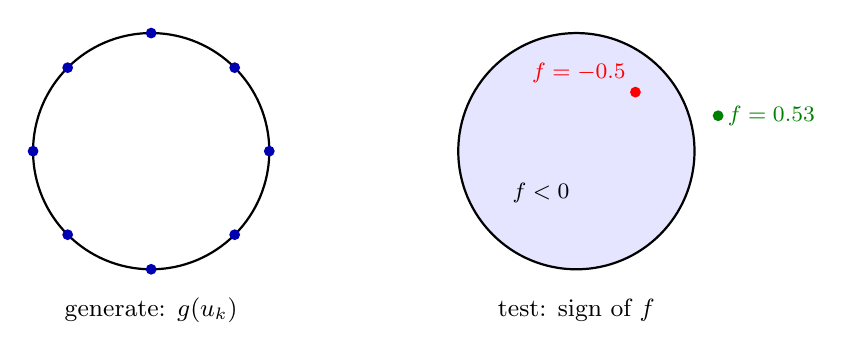
\begin{tikzpicture}[font=\small,scale=1.5]
\draw[thick] (0,0) circle (1);
\foreach \i in {0,...,7}{\fill[blue!70!black] (45*\i:1) circle (1.3pt);}
\node at (0,-1.35) {generate: $g(u_k)$};
\begin{scope}[xshift=3.6cm]
\fill[blue!10] (0,0) circle (1);
\draw[thick] (0,0) circle (1);
\fill[red] (0.5,0.5) circle (1.3pt) node[above left,font=\footnotesize] {$f=-0.5$};
\fill[green!50!black] (1.2,0.3) circle (1.3pt) node[right,font=\footnotesize] {$f=0.53$};
\node[font=\footnotesize] at (-0.3,-0.35) {$f<0$};
\node at (0,-1.35) {test: sign of $f$};
\end{scope}
\end{tikzpicture}
\caption{Left: the parametric circle produces points. Right: the implicit circle classifies any point by the sign of $f$.}
\end{figure}

\begin{intuition}
Parametric $\approx$ a machine that \emph{prints} surface points; implicit $\approx$ a \emph{bouncer} that checks tickets. Printing 100 points is trivial with the printer and awkward with the bouncer (you have to hunt for the zeros); checking a single point is trivial with the bouncer and awkward with the printer (you must invert $g$).
\end{intuition}

\subsection{Implicit Surfaces: Examples \slides{slide 49}}
Simple functions can give concise representations of complex shapes:
\begin{align*}
\text{sphere:}\quad & f(x,y,z)=x^2+y^2+z^2-1,\\
\text{torus:}\quad & f(x,y,z)=(x^2+y^2+z^2+R^2-a^2)^2-4R^2(x^2+y^2),\\
\text{quartic (blob with a hole):}\quad & f(x,y,z)=x^4+y^4+z^4+2x^2y^2+2x^2z^2\\
& \qquad\quad{}+2y^2z^2+8xyz-10x^2-10y^2-10z^2+20.
\end{align*}

\begin{figure}[H]
\centering
\includegraphics[width=0.75\textwidth]{implicit_examples.png}
\caption{Implicit surfaces: sphere, torus, and a quartic with a hole. The last one is a single polynomial of degree 4, yet it has a hole in it.}
\end{figure}

\subsection{When a Field Defines a Surface \slides{slide 50}}
Not every field defines a surface. Four test cases (with $r=\norm{\vx}$):
\begin{center}
\begin{tabular}{lll}
\toprule
$f(\vx)$ & zero set & a surface?\\
\midrule
$\norm{\vx}-1$ & unit sphere & yes\\
$\norm{\vx}^2+1$ & empty & no, there is nothing there\\
$\norm{\vx}^2$ & the origin & no, a single point\\
$(\norm{\vx}-1)^2$ & unit sphere & no: $f\ge0$ everywhere, so no inside, and $\nabla f=0$ on it\\
\bottomrule
\end{tabular}
\end{center}

\begin{proposition}[When $f$ defines a surface]
$f$ must change sign across $\Surf$, and $\nabla f\ne 0$ on $\Surf$. (If $f$ is continuously differentiable and $\nabla f\neq0$ at every zero of $f$, the implicit function theorem shows that $\Surf$ is locally the graph of a smooth function, i.e.\ a smooth surface.)
\end{proposition}

\begin{figure}[ht]
\centering
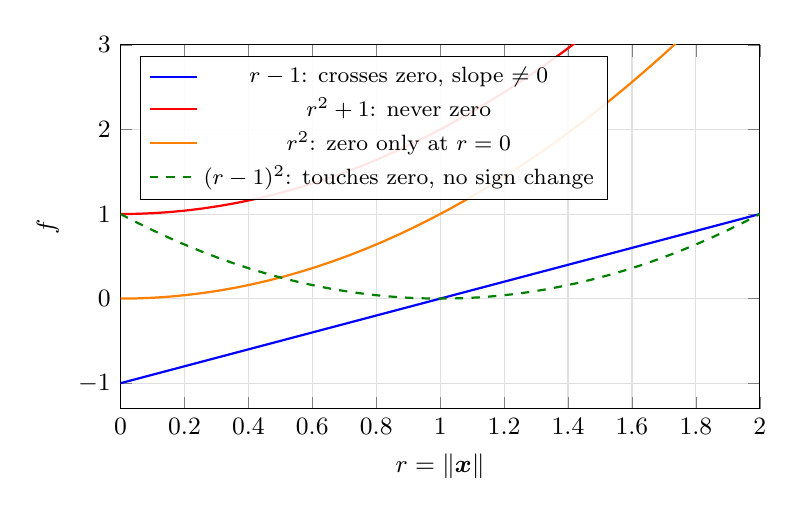
\begin{tikzpicture}
\begin{axis}[width=0.8\linewidth,height=6.2cm,xlabel={$r=\norm{\vx}$},ylabel={$f$},xmin=0,xmax=2,ymin=-1.3,ymax=3,grid=both,legend pos=north west,legend style={font=\footnotesize,fill=white,fill opacity=0.9,text opacity=1,draw opacity=1}]
\addplot[thick,blue,domain=0:2,samples=2] {x-1}; \addlegendentry{$r-1$: crosses zero, slope $\ne0$}
\addplot[thick,red,domain=0:2,samples=40] {x^2+1}; \addlegendentry{$r^2+1$: never zero}
\addplot[thick,orange,domain=0:2,samples=40] {x^2}; \addlegendentry{$r^2$: zero only at $r=0$}
\addplot[thick,green!50!black,dashed,domain=0:2,samples=40] {(x-1)^2}; \addlegendentry{$(r-1)^2$: touches zero, no sign change}
\end{axis}
\end{tikzpicture}
\caption{Radial profiles of the four candidate fields. Only the first one changes sign at the unit sphere with a non-zero slope.}
\end{figure}

\begin{intuition}
A surface is where the field \emph{crosses} zero, like the shoreline where altitude crosses sea level. A field that only touches zero (the last row) gives a double root: no ``inside'', no well-defined normal. A field that never reaches zero gives nothing.
\end{intuition}

\subsection{Normals for Free \slides{slide 51}}
\begin{lemma}[Normal of an implicit surface]
The gradient is perpendicular to the level sets, so on the surface
\[
\vn(\vx)=\frac{\nabla f(\vx)}{\norm{\nabla f(\vx)}}.
\]
It points toward increasing $f$, which by our convention is \emph{outward}.
\end{lemma}
\begin{proof}
Let $\gamma(t)$ be any curve lying in $\Surf$. Then $f(\gamma(t))=0$ for all $t$; differentiating, $\nabla f(\gamma(t))\cdot\gamma'(t)=0$, so $\nabla f$ is orthogonal to every tangent direction of the surface.
\end{proof}

For the sphere, $\nabla f=2\vx$ and $\vn=\vx/\norm{\vx}$. With automatic differentiation the normals of \emph{any} differentiable $f$ (an MLP, say) come for free:
\begin{lstlisting}
x = pts.clone().requires_grad_(True)            # (N, 3) points
v = f(x)                                        # any differentiable f, e.g. an MLP
g, = torch.autograd.grad(v.sum(), x)
n = g / g.norm(dim=-1, keepdim=True)            # (N, 3) unit normals
\end{lstlisting}

\begin{figure}[ht]
\centering
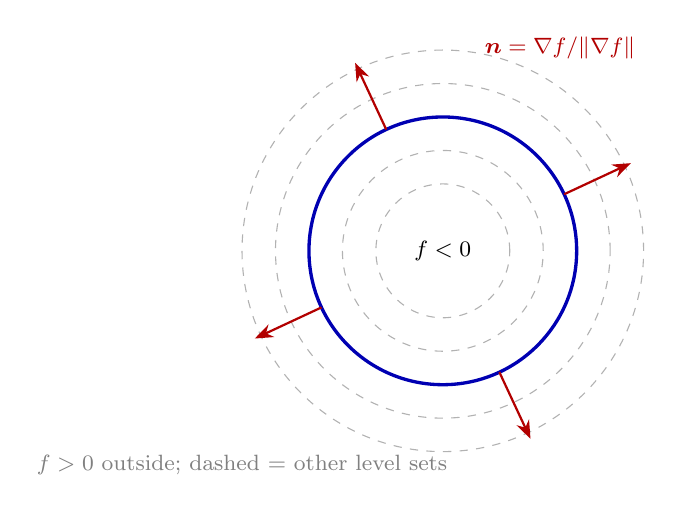
\begin{tikzpicture}[font=\small,>=Stealth,scale=1.7]
\foreach \r in {0.5,0.75,1.25,1.5}{\draw[gray!60,dashed] (0,0) circle (\r);}
\draw[very thick,blue!70!black] (0,0) circle (1);
\foreach \a in {25,115,205,295}{\draw[->,thick,red!70!black] (\a:1) -- (\a:1.55);}
\node[red!70!black,font=\footnotesize] at (60:1.75) {$\vn=\nabla f/\norm{\nabla f}$};
\node[font=\footnotesize] at (0,0) {$f<0$};
\node[font=\footnotesize,gray] at (-1.5,-1.6) {$f>0$ outside; dashed = other level sets};
\end{tikzpicture}
\caption{The gradient of $f$ is orthogonal to the level sets and points toward larger $f$, i.e.\ out of the shape.}
\end{figure}

\begin{intuition}
Picture $f$ as terrain height and the surface as the zero contour line. The gradient points straight uphill, perpendicular to any contour line: that is the normal. No separate normal array has to be stored or kept consistent, unlike the per-face orientation of a mesh.
\end{intuition}

\subsection{Boolean Operations \slides{slide 52}}
\begin{proposition}[Booleans via $\min$ and $\max$]
With $f<0$ inside,
\[
f_{A\cup B}=\min(f_A,f_B),\qquad f_{A\cap B}=\max(f_A,f_B),\qquad f_{A\setminus B}=\max(f_A,-f_B).
\]
\end{proposition}
\begin{proof}
$\vx\in A\cup B\iff f_A(\vx)<0$ or $f_B(\vx)<0\iff\min(f_A,f_B)<0$. Likewise $\vx\in A\cap B\iff f_A<0$ and $f_B<0\iff\max(f_A,f_B)<0$. For $A\setminus B=A\cap B^{c}$, the complement of $B$ is described (up to its boundary) by $-f_B<0$, so $\max(f_A,-f_B)<0$.
\end{proof}

\begin{figure}[ht]
\centering
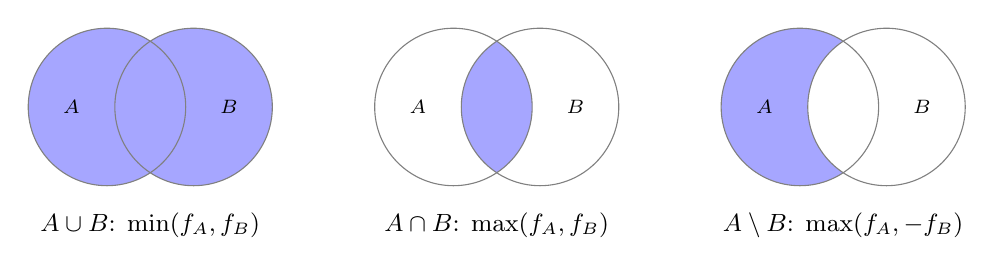
\begin{tikzpicture}[font=\small]
\foreach \dx/\k/\t in {0/0/{$A\cup B$: $\min(f_A,f_B)$},4.4/1/{$A\cap B$: $\max(f_A,f_B)$},8.8/2/{$A\setminus B$: $\max(f_A,-f_B)$}}{
 \begin{scope}[xshift=\dx cm]
 \ifnum\k=0 \fill[blue!35] (0,0) circle (1) (1.1,0) circle (1); \fi
 \ifnum\k=1 \begin{scope}\clip (0,0) circle (1); \fill[blue!35] (1.1,0) circle (1);\end{scope} \fi
 \ifnum\k=2 \begin{scope}\clip (0,0) circle (1); \begin{scope}[even odd rule]\clip (-3,-3) rectangle (4,3) (1.1,0) circle (1); \fill[blue!35] (-3,-3) rectangle (4,3);\end{scope}\end{scope} \fi
 \draw[gray] (0,0) circle (1); \draw[gray] (1.1,0) circle (1);
 \node at (-0.45,0) {\scriptsize $A$}; \node at (1.55,0) {\scriptsize $B$};
 \node at (0.55,-1.5) {\t};
 \end{scope}
}
\end{tikzpicture}
\caption{2D versions of the three Boolean operations (blue = result).}
\end{figure}

\begin{intuition}
``Inside the union'' means ``inside at least one'': the most negative of the two values decides, hence $\min$. ``Inside the intersection'' needs both, so the \emph{least} negative value decides: $\max$. Subtraction is intersection with the outside of $B$, and flipping the sign of $f_B$ swaps inside and outside. The \emph{sign} of the result is always correct; the magnitude near sharp creases is not guaranteed to remain an exact distance (see the SDF discussion next).
\end{intuition}

\subsection{Many Functions, One Surface \slides{slide 53}}
The surface does not fix $f$: many different fields have the same zero set. So one can choose an $f$ that is useful \emph{away} from the surface.

\subsection{Signed Distance Function \slides{slides 54--58}}
\begin{definition}[Signed distance function (SDF)]
\[
f(\vx)=\begin{cases}-\dist(\vx,\Surf)&\vx\text{ inside}\\ +\dist(\vx,\Surf)&\vx\text{ outside}\end{cases},\qquad \dist(\vx,\Surf)=\min_{\vy\in\Surf}\norm{\vx-\vy}.
\]
\end{definition}

Which of the fields of slide 55 are SDFs? $x^2+y^2+z^2-1$ and the quartic of slide 49: \emph{neither}!

\begin{proposition}[Eikonal condition]\label{prop:eikonal}
An SDF satisfies $\norm{\nabla f}=1$ (wherever it is differentiable).
\end{proposition}
\begin{proof}
Take a small step of length $\delta$ from a point. In \emph{any} direction the distance to the surface changes by at most $\delta$; stepping straight away from the closest surface point it changes by exactly $\delta$. So the steepest slope of $f$ is exactly one.
\end{proof}

\begin{example}
$f=\norm{\vx}-1$: $\nabla f=\vx/\norm{\vx}$, $\norm{\nabla f}=1$, an SDF. $f=\norm{\vx}^2-1$: $\nabla f=2\vx$, $\norm{\nabla f}=2\norm{\vx}\ne1$, not an SDF.
\end{example}

\begin{figure}[ht]
\centering
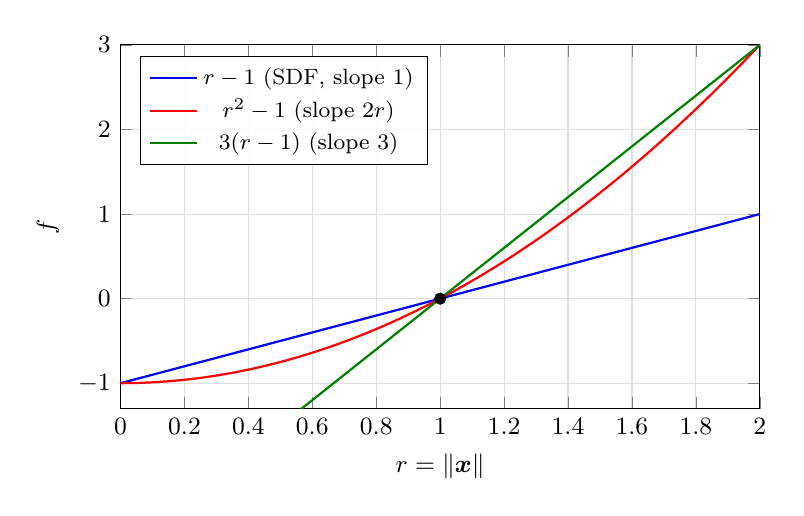
\begin{tikzpicture}
\begin{axis}[width=0.8\linewidth,height=6.2cm,xlabel={$r=\norm{\vx}$},ylabel={$f$},xmin=0,xmax=2,ymin=-1.3,ymax=3,grid=both,legend pos=north west,legend style={font=\footnotesize,fill=white,fill opacity=0.9,text opacity=1,draw opacity=1}]
\addplot[thick,blue,domain=0:2,samples=2] {x-1}; \addlegendentry{$r-1$ (SDF, slope 1)}
\addplot[thick,red,domain=0:2,samples=40] {x^2-1}; \addlegendentry{$r^2-1$ (slope $2r$)}
\addplot[thick,green!50!black,domain=0:2,samples=2] {3*(x-1)}; \addlegendentry{$3(r-1)$ (slope 3)}
\addplot[only marks,mark=*,black] coordinates {(1,0)};
\end{axis}
\end{tikzpicture}
\caption{Three fields with the same zero set (the unit sphere, $r=1$). Only the slope-one profile is a signed distance function.}
\end{figure}

\begin{intuition}
The eikonal condition says ``the field grows like a ruler as you walk away from the surface''. An SDF is the most \emph{honest} field: its value literally is the distance to the surface. The other fields agree on \emph{where} the surface is but exaggerate or shrink the distances; $r^2-1$ overstates by the factor $r+1$ at radius $r$.
\end{intuition}

\paragraph{Why honesty matters: safe steps \slides{slides 57--58}.}
\begin{proposition}[Safe step]
If $f$ is an SDF, the ball of radius $\abs{f(\vx)}$ around $\vx$ contains no surface point in its interior. Hence a ray can safely advance by $\abs{f(\vx)}$. If $f$ overstates the distance, the ball can cross the surface and stepping by $f$ can \emph{jump through} it.
\end{proposition}
\begin{proof}
By definition $\abs{f(\vx)}=\dist(\vx,\Surf)$, the radius of the largest ball around $\vx$ that avoids $\Surf$. For a non-SDF field the ball of radius $\abs{f}$ can be larger than $\dist(\vx,\Surf)$ and then contains surface points.
\end{proof}

\begin{example}[Slides 57--58, $\vx$ at $r\approx2.67$]
For $f=r^2-1$: $f=6.14$, true distance $1.67$, $\norm{\nabla f}=5.34$: the circle of radius $\abs f$ crosses the surface. For an SDF at the same point the ball of radius $r-1=1.67$ touches the surface without crossing.
\end{example}

\begin{figure}[ht]
\centering
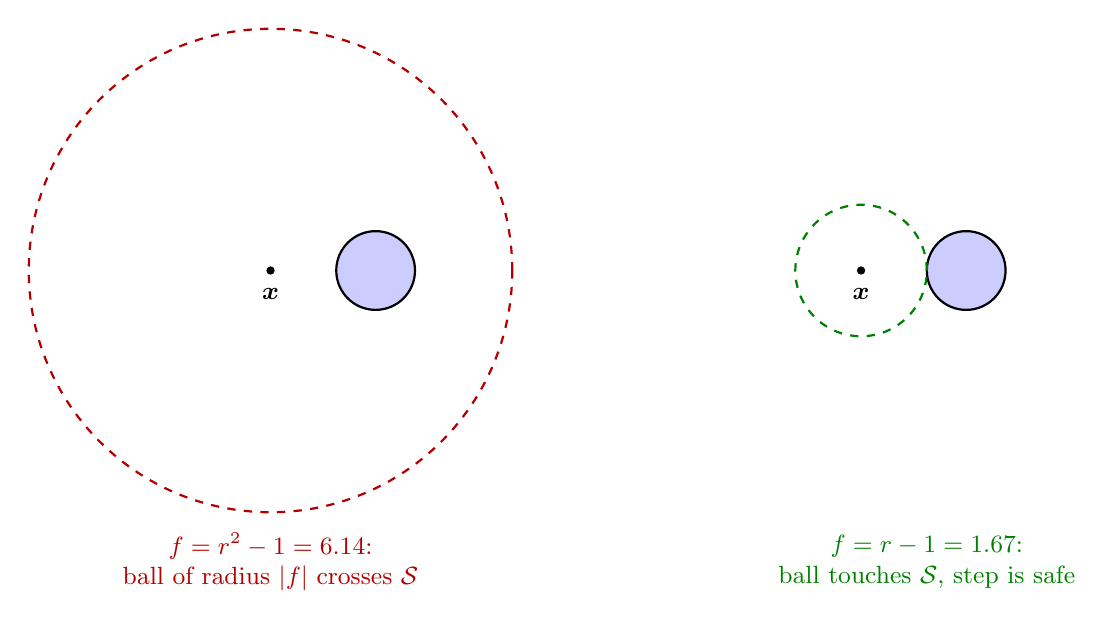
\begin{tikzpicture}[font=\small,scale=0.5]
\begin{scope}
\fill[blue!20] (0,0) circle (1); \draw[thick] (0,0) circle (1);
\draw[dashed,red!70!black,thick] (-2.67,0) circle (6.14);
\fill (-2.67,0) circle (3pt); \node[below] at (-2.67,-0.2) {$\vx$};
\node[red!70!black,align=center] at (-2.67,-7.4) {$f=r^2-1=6.14$:\\ball of radius $|f|$ crosses $\Surf$};
\end{scope}
\begin{scope}[xshift=15cm]
\fill[blue!20] (0,0) circle (1); \draw[thick] (0,0) circle (1);
\draw[dashed,green!50!black,thick] (-2.67,0) circle (1.67);
\fill (-2.67,0) circle (3pt); \node[below] at (-2.67,-0.2) {$\vx$};
\node[green!50!black,align=center] at (-1,-7.4) {$f=r-1=1.67$:\\ball touches $\Surf$, step is safe};
\end{scope}
\end{tikzpicture}
\caption{The same point $\vx$ with two fields that define the same sphere. Left: stepping by $f=r^2-1$ overshoots. Right: an SDF gives the largest safe step.}
\end{figure}

\begin{algorithm}[Sphere tracing / ray marching an SDF]
Given a ray $\vo+t\vd$ ($\norm{\vd}=1$) and an SDF $f$: set $t\leftarrow0$; repeat $t\leftarrow t+f(\vo+t\vd)$ until $f<\varepsilon$ (hit) or $t$ exceeds a maximum (miss).
\end{algorithm}

\begin{figure}[ht]
\centering
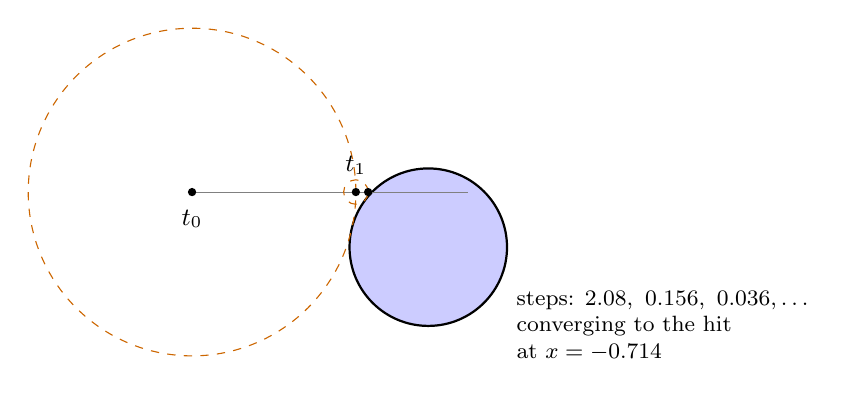
\begin{tikzpicture}[font=\small,>=Stealth]
\fill[blue!20] (0,0) circle (1); \draw[thick] (0,0) circle (1);
\draw[gray] (-3,0.7) -- (0.5,0.7);
\draw[dashed,orange!80!black] (-3,0.7) circle (2.0806);
\draw[dashed,orange!80!black] (-0.9194,0.7) circle (0.1556);
\draw[dashed,orange!80!black] (-0.7638,0.7) circle (0.0361);
\foreach \x in {-3,-0.9194,-0.7638}{\fill (\x,0.7) circle (1.5pt);}
\node[below] at (-3,0.6) {$t_0$}; \node[above] at (-0.9194,0.8) {$t_1$};
\node[align=left,font=\footnotesize] at (3,-1.0) {steps: $2.08,\ 0.156,\ 0.036,\dots$\\converging to the hit\\at $x=-0.714$};
\end{tikzpicture}
\caption{Sphere tracing a horizontal ray at height $0.7$ against the unit sphere: each step is the SDF value, the radius of the empty ball.}
\end{figure}

\begin{intuition}
It is like walking through fog toward a wall with a distance meter: if the meter never lies (SDF) you can always walk the displayed distance without hitting the wall, and the steps shrink as you approach. A meter that overstates makes you walk into and through the wall. This is why the table on slide 66 lists ``ray marching'' as the way to render implicit surfaces.
\end{intuition}

\subsection{Storing a Field on a Grid \slides{slide 59}}
Store samples $F[i,j,k]=f(\vx_{ijk})$ at the grid points and interpolate in between: the same data structure as a voxel grid, but holding \emph{signed distances} rather than occupancy. A \emph{TSDF} keeps values only near the surface and clamps them to $\pm\tau$ elsewhere, $f_\tau=\clamp(f,-\tau,\tau)$; it is the standard way to fuse many depth maps into one model, as in KinectFusion.
\begin{lstlisting}
xs = np.linspace(-1.5, 1.5, 128)
X, Y, Z = np.meshgrid(xs, xs, xs, indexing="ij")
F = np.sqrt(X**2 + Y**2 + Z**2) - 1.0           # unit-sphere SDF on a 128^3 grid
\end{lstlisting}

\begin{intuition}
The grid now stores \emph{how far} each cell is from the surface instead of \emph{whether} it is occupied. Values change smoothly across the surface, so interpolation places the surface at sub-voxel accuracy, and the clamped version stores only what matters: a thin shell around the surface.
\end{intuition}

\subsection{Storing a Field in a Network \slides{slide 60}}
$\{\vx\mid f_\theta(\vx)=0\}$, with $f_\theta$ a small MLP (three numbers in, one out). Two requirements: $f_\theta(\vx_i)\approx0$ on the data points (the surface passes through the data), and $\norm{\nabla f_\theta(\vx)}\approx1$ everywhere (it behaves like an SDF). Resolution is not tied to a grid.

\begin{figure}[H]
\centering
\includegraphics[width=0.75\textwidth]{implicit_network.png}
\caption{A small MLP can represent a continuous field $f_\theta$, whose zero set is the surface.}
\end{figure}

\begin{example}[One way to write the two requirements as a loss]
$\mathcal L(\theta)=\frac1N\sum_i\abs{f_\theta(\vx_i)}+\lambda\,\mathbb E_{\vx}\big[(\norm{\nabla f_\theta(\vx)}-1)^2\big]$. The first term pulls the zero set through the samples; the second is the eikonal penalty of Proposition~\ref{prop:eikonal}.
\end{example}

\begin{intuition}
The network is a \emph{compressed}, resolution-free grid: query it at any point, at any density. The eikonal penalty is what stops the network from producing an arbitrary function that merely vanishes on the data.
\end{intuition}

\subsection{From Implicit Surface to Mesh \slides{slide 61}}

\begin{figure}[H]
\centering
\includegraphics[width=0.75\textwidth]{marching_squares.png}
\caption{Marching squares (the 2D version of marching cubes) in one cell. The blue corners are inside ($f<0$),the white corners are outside ($f>0$). The dotted line is the true surface; the orange line is the interpolated surface from marching squares.}
\end{figure}
\begin{algorithm}[Marching cubes]\label{alg:mc}
\textbf{1.}~Evaluate $f$ on a grid (analytic, a TSDF, or a network).\\
\textbf{2.}~Find the cells whose corners differ in sign.\\
\textbf{3.}~On each such edge $[\va,\vb]$, place a vertex at the zero crossing
$p=\va+t(\vb-\va)$ with $t=\dfrac{f(\va)}{f(\va)-f(\vb)}$.\\
\textbf{4.}~In 3D, join the vertices with a lookup table on the corner signs: $2^8$ cases per cube.
\end{algorithm}

\begin{lstlisting}
from skimage.measure import marching_cubes
h = xs[1] - xs[0]                                # voxel size, from the grid above
verts, faces, normals, _ = marching_cubes(F, level=0.0, spacing=(h, h, h))
verts += xs[0]                                   # grid -> world coordinates
\end{lstlisting}

\begin{figure}[ht]
\centering
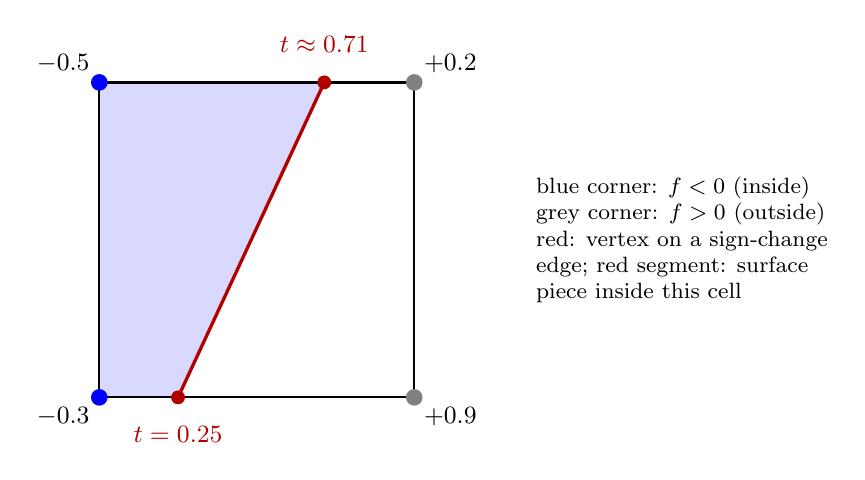
\begin{tikzpicture}[font=\small]
\fill[blue!15] (0,0)--(1,0)--(2.857,4)--(0,4)--cycle;
\draw[thick] (0,0) rectangle (4,4);
\draw[very thick,red!70!black] (1,0)--(2.857,4);
\fill[blue] (0,0) circle (3pt); \fill[blue] (0,4) circle (3pt);
\fill[gray] (4,0) circle (3pt); \fill[gray] (4,4) circle (3pt);
\node[below left] at (0,0) {$-0.3$}; \node[below right] at (4,0) {$+0.9$};
\node[above left] at (0,4) {$-0.5$}; \node[above right] at (4,4) {$+0.2$};
\fill[red!70!black] (1,0) circle (2.5pt); \fill[red!70!black] (2.857,4) circle (2.5pt);
\node[below,red!70!black] at (1,-0.25) {$t=0.25$}; \node[above,red!70!black] at (2.857,4.25) {$t\approx0.71$};
\node[align=left,font=\footnotesize] at (7.4,2) {blue corner: $f<0$ (inside)\\grey corner: $f>0$ (outside)\\red: vertex on a sign-change\\edge; red segment: surface\\piece inside this cell};
\end{tikzpicture}
\caption{Marching squares (the 2D version of marching cubes) in one cell. On the bottom edge $t=\frac{-0.3}{-0.3-0.9}=0.25$; on the top edge $t=\frac{-0.5}{-0.5-0.2}\approx0.71$. The left and right edges have no sign change, hence no vertex.}
\end{figure}

\begin{intuition}
Marching cubes is ``connect the dots along the shoreline'': the corner signs say which cell edges the coastline crosses; linear interpolation of $f$ along that edge says \emph{where} (a corner with a small $|f|$ is close to the surface, so the vertex sits close to it). This is the bridge from implicit to mesh, which is what GPUs render.
\end{intuition}

\subsection{Implicit Surfaces: Summary \slides{slide 62}}
\begin{center}
\begin{tabular}{L{6.6cm}L{6.6cm}}
\toprule
\textbf{Easy} & \textbf{Hard}\\
\midrule
inside or outside: the sign of $f$ & getting points on the surface\\
any topology, changing continuously & no direct rasterization\\
booleans: a $\min$ or a $\max$ & an arbitrary $f$ may define nothing\\
normals: $\nabla f$ & \\
\bottomrule
\end{tabular}
\end{center}
The mirror image of parametric surfaces.

% =====================================================================
\section{Boundary vs Volumetric Representations \slides{slide 63}}
% =====================================================================
Slide 63 summarizes the two families: \emph{boundary} representations for shapes (point clouds, meshes, parametric surfaces) and \emph{volumetric} representations for shapes (voxels, implicit fields).

% =====================================================================
\section{Density Fields \slides{slides 64--65}}
% =====================================================================
\subsection{Density fields \slides{slide 64}}
Occupancy asks ``is this point inside?''; density asks ``how opaque is this point?''.

\begin{figure}[H]
\centering
\includegraphics[width=0.75\textwidth]{density_field.png}
\caption{Two images examples}
\end{figure}
\begin{definition}[Density field]
A density field assigns $\sigma(\vx)\in\R^+$ (or $\sigma[i,j,k]\in\R^+$ on a grid); $\sigma(\vx)\ge0$ says how much light is absorbed per unit length at $\vx$.
\end{definition}

There is no notion of a surface: e.g.\ $\sigma(\vx)=0.1$ everywhere represents a semi-transparent fluid. Typical examples on the slide: smoke and CT-scan slices. The lecture will revisit this in more detail later (NeRF).

\begin{example}[Preview: how much light survives?]
If a beam crosses a slab of length $L$ of constant density $\sigma$, the fraction of light transmitted is $e^{-\sigma L}$ (absorption per unit length compounds multiplicatively). For $\sigma=0.1$ and $L=10$: $e^{-1}\approx0.37$. (This is a standard consequence of the ``absorbed per unit length'' reading; the slides develop it later.)
\end{example}

\subsection{Primitive-based Density Fields \slides{slide 65}}
\[
\sigma(\vx)=\sum_k w_k\exp\!\Big(-\tfrac12(\vx-\vmu_k)^{\!\top}\Sigma_k^{-1}(\vx-\vmu_k)\Big).
\]
These are \emph{hybrid} representations for primitive-induced density fields (blobs/Gaussians with weights $w_k$, centres $\vmu_k$, covariances $\Sigma_k$); the lecture will revisit them in more detail (differentiable Gaussian rendering).
\begin{figure}[H]
\centering
\includegraphics[width=0.75\textwidth]{density_fields_example.png}
\caption{Images examples of primitive-based density fields}
\end{figure}

\begin{intuition}
Instead of a grid of numbers, the density is a \emph{cloud of soft blobs}: each blob has a position, a size/orientation (via $\Sigma_k$) and a weight. The whole field can be edited by moving blobs, and only regions with blobs cost anything, so it avoids the ``pay for empty space'' problem of dense grids.
\end{intuition}

% =====================================================================
\section{So? \slides{slide 66}}
% =====================================================================
Slide 66 compares the representations side by side (its cells are colour-coded easy / possible with effort / hard; the colours do not survive in the text of the PDF, so the qualitative ratings appear in Section~\ref{sec:summary}, based on the earlier slides):

\begin{center}
\small
\renewcommand{\arraystretch}{1.25}
\setlength{\tabcolsep}{3pt}\begin{tabular}{L{2.2cm}L{2.4cm}L{2.3cm}L{2.4cm}L{2.1cm}L{2.5cm}}
\toprule
 & \textbf{Points on the surface} & \textbf{Inside or outside?} & \textbf{Continuous edits reach} & \textbf{Rendering} & \textbf{Typical use}\\
\midrule
\textbf{Point cloud} (array $N\times3$) & given & no surface & any point set & splats & sensors: LiDAR, RGB-D\\
\textbf{Mesh} ($V:N\times3$, $F:M\times3$) & sample triangles & count ray crossings & same wiring only & GPU rasterizer & graphics, games\\
\textbf{Parametric} ($f(\vu)$) & evaluate $f$ & search over $\vu$ & same topology only & via a mesh & CAD, design\\
\textbf{Voxels} (grid $W\times H\times D$) & marching cubes & look up the cell & any topology* & blocky & 3D CNNs, occupancy maps\\
\textbf{Implicit (SDF)} ($f(\vx)$: formula, grid, net) & marching cubes & sign of $f$ & any topology & ray marching & reconstruction, neural fields\\
\bottomrule
\end{tabular}
\end{center}
{\small * with occupancy probabilities, not $0$ or $1$.}

\begin{intuition}
\emph{No row wins every column: pick the representation for the task.} Need to shoot rays fast on a GPU? Mesh. Need to change topology or run inside/outside queries? Implicit. Data straight from a LiDAR? Points. Feeding a 3D CNN? Voxels.
\end{intuition}

% =====================================================================
\section{And many more\dots\ \slides{slides 67--71}}
% =====================================================================

\subsection{Octrees \slides{slide 68}}
Octrees are \emph{voxels with adaptive resolution}: surface-like efficiency for rendering and storage, volume-like efficiency for occupancy queries; but it is difficult to edit or predict the sparsity structure.

\begin{figure}[ht]
\centering
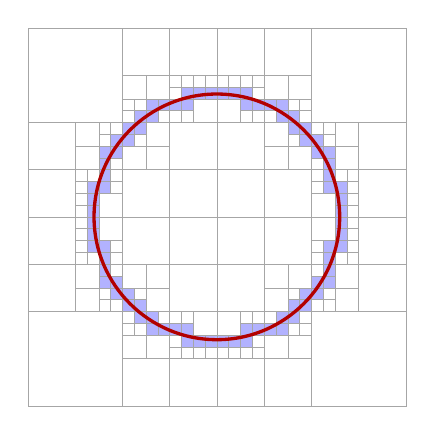
\begin{tikzpicture}[scale=2.4]
\fill[blue!30] (-0.5625,-0.4375) rectangle (-0.5000,-0.3750);
\fill[blue!30] (-0.6250,-0.3750) rectangle (-0.5625,-0.3125);
\fill[blue!30] (-0.6250,-0.3125) rectangle (-0.5625,-0.2500);
\fill[blue!30] (-0.5625,-0.3750) rectangle (-0.5000,-0.3125);
\fill[blue!30] (-0.6875,-0.1875) rectangle (-0.6250,-0.1250);
\fill[blue!30] (-0.6875,-0.1250) rectangle (-0.6250,-0.0625);
\fill[blue!30] (-0.6875,-0.0625) rectangle (-0.6250,0.0000);
\fill[blue!30] (-0.6250,-0.2500) rectangle (-0.5625,-0.1875);
\fill[blue!30] (-0.6250,-0.1875) rectangle (-0.5625,-0.1250);
\fill[blue!30] (-0.4375,-0.5625) rectangle (-0.3750,-0.5000);
\fill[blue!30] (-0.3750,-0.6250) rectangle (-0.3125,-0.5625);
\fill[blue!30] (-0.3750,-0.5625) rectangle (-0.3125,-0.5000);
\fill[blue!30] (-0.3125,-0.6250) rectangle (-0.2500,-0.5625);
\fill[blue!30] (-0.1875,-0.6875) rectangle (-0.1250,-0.6250);
\fill[blue!30] (-0.2500,-0.6250) rectangle (-0.1875,-0.5625);
\fill[blue!30] (-0.1875,-0.6250) rectangle (-0.1250,-0.5625);
\fill[blue!30] (-0.1250,-0.6875) rectangle (-0.0625,-0.6250);
\fill[blue!30] (-0.0625,-0.6875) rectangle (0.0000,-0.6250);
\fill[blue!30] (-0.5000,-0.5000) rectangle (-0.4375,-0.4375);
\fill[blue!30] (-0.5000,-0.4375) rectangle (-0.4375,-0.3750);
\fill[blue!30] (-0.4375,-0.5000) rectangle (-0.3750,-0.4375);
\fill[blue!30] (-0.6875,0.0000) rectangle (-0.6250,0.0625);
\fill[blue!30] (-0.6875,0.0625) rectangle (-0.6250,0.1250);
\fill[blue!30] (-0.6875,0.1250) rectangle (-0.6250,0.1875);
\fill[blue!30] (-0.6250,0.1250) rectangle (-0.5625,0.1875);
\fill[blue!30] (-0.6250,0.1875) rectangle (-0.5625,0.2500);
\fill[blue!30] (-0.6250,0.2500) rectangle (-0.5625,0.3125);
\fill[blue!30] (-0.6250,0.3125) rectangle (-0.5625,0.3750);
\fill[blue!30] (-0.5625,0.3125) rectangle (-0.5000,0.3750);
\fill[blue!30] (-0.5625,0.3750) rectangle (-0.5000,0.4375);
\fill[blue!30] (-0.5000,0.3750) rectangle (-0.4375,0.4375);
\fill[blue!30] (-0.5000,0.4375) rectangle (-0.4375,0.5000);
\fill[blue!30] (-0.4375,0.4375) rectangle (-0.3750,0.5000);
\fill[blue!30] (-0.4375,0.5000) rectangle (-0.3750,0.5625);
\fill[blue!30] (-0.3750,0.5000) rectangle (-0.3125,0.5625);
\fill[blue!30] (-0.3750,0.5625) rectangle (-0.3125,0.6250);
\fill[blue!30] (-0.3125,0.5625) rectangle (-0.2500,0.6250);
\fill[blue!30] (-0.2500,0.5625) rectangle (-0.1875,0.6250);
\fill[blue!30] (-0.1875,0.5625) rectangle (-0.1250,0.6250);
\fill[blue!30] (-0.1875,0.6250) rectangle (-0.1250,0.6875);
\fill[blue!30] (-0.1250,0.6250) rectangle (-0.0625,0.6875);
\fill[blue!30] (-0.0625,0.6250) rectangle (0.0000,0.6875);
\fill[blue!30] (0.0000,-0.6875) rectangle (0.0625,-0.6250);
\fill[blue!30] (0.0625,-0.6875) rectangle (0.1250,-0.6250);
\fill[blue!30] (0.1250,-0.6875) rectangle (0.1875,-0.6250);
\fill[blue!30] (0.1250,-0.6250) rectangle (0.1875,-0.5625);
\fill[blue!30] (0.1875,-0.6250) rectangle (0.2500,-0.5625);
\fill[blue!30] (0.2500,-0.6250) rectangle (0.3125,-0.5625);
\fill[blue!30] (0.3125,-0.6250) rectangle (0.3750,-0.5625);
\fill[blue!30] (0.3125,-0.5625) rectangle (0.3750,-0.5000);
\fill[blue!30] (0.3750,-0.5625) rectangle (0.4375,-0.5000);
\fill[blue!30] (0.3750,-0.5000) rectangle (0.4375,-0.4375);
\fill[blue!30] (0.4375,-0.5000) rectangle (0.5000,-0.4375);
\fill[blue!30] (0.4375,-0.4375) rectangle (0.5000,-0.3750);
\fill[blue!30] (0.5000,-0.4375) rectangle (0.5625,-0.3750);
\fill[blue!30] (0.5000,-0.3750) rectangle (0.5625,-0.3125);
\fill[blue!30] (0.5625,-0.3750) rectangle (0.6250,-0.3125);
\fill[blue!30] (0.5625,-0.3125) rectangle (0.6250,-0.2500);
\fill[blue!30] (0.5625,-0.2500) rectangle (0.6250,-0.1875);
\fill[blue!30] (0.5625,-0.1875) rectangle (0.6250,-0.1250);
\fill[blue!30] (0.6250,-0.1875) rectangle (0.6875,-0.1250);
\fill[blue!30] (0.6250,-0.1250) rectangle (0.6875,-0.0625);
\fill[blue!30] (0.6250,-0.0625) rectangle (0.6875,0.0000);
\fill[blue!30] (0.3750,0.4375) rectangle (0.4375,0.5000);
\fill[blue!30] (0.4375,0.3750) rectangle (0.5000,0.4375);
\fill[blue!30] (0.4375,0.4375) rectangle (0.5000,0.5000);
\fill[blue!30] (0.0000,0.6250) rectangle (0.0625,0.6875);
\fill[blue!30] (0.0625,0.6250) rectangle (0.1250,0.6875);
\fill[blue!30] (0.1250,0.5625) rectangle (0.1875,0.6250);
\fill[blue!30] (0.1875,0.5625) rectangle (0.2500,0.6250);
\fill[blue!30] (0.1250,0.6250) rectangle (0.1875,0.6875);
\fill[blue!30] (0.2500,0.5625) rectangle (0.3125,0.6250);
\fill[blue!30] (0.3125,0.5000) rectangle (0.3750,0.5625);
\fill[blue!30] (0.3125,0.5625) rectangle (0.3750,0.6250);
\fill[blue!30] (0.3750,0.5000) rectangle (0.4375,0.5625);
\fill[blue!30] (0.5625,0.1250) rectangle (0.6250,0.1875);
\fill[blue!30] (0.5625,0.1875) rectangle (0.6250,0.2500);
\fill[blue!30] (0.6250,0.0000) rectangle (0.6875,0.0625);
\fill[blue!30] (0.6250,0.0625) rectangle (0.6875,0.1250);
\fill[blue!30] (0.6250,0.1250) rectangle (0.6875,0.1875);
\fill[blue!30] (0.5000,0.3125) rectangle (0.5625,0.3750);
\fill[blue!30] (0.5625,0.2500) rectangle (0.6250,0.3125);
\fill[blue!30] (0.5625,0.3125) rectangle (0.6250,0.3750);
\fill[blue!30] (0.5000,0.3750) rectangle (0.5625,0.4375);
\draw[gray!70,line width=0.15pt] (-1.0000,-1.0000) rectangle (-0.5000,-0.5000);
\draw[gray!70,line width=0.15pt] (-1.0000,-0.5000) rectangle (-0.7500,-0.2500);
\draw[gray!70,line width=0.15pt] (-1.0000,-0.2500) rectangle (-0.7500,0.0000);
\draw[gray!70,line width=0.15pt] (-0.7500,-0.5000) rectangle (-0.6250,-0.3750);
\draw[gray!70,line width=0.15pt] (-0.7500,-0.3750) rectangle (-0.6250,-0.2500);
\draw[gray!70,line width=0.15pt] (-0.6250,-0.5000) rectangle (-0.5625,-0.4375);
\draw[gray!70,line width=0.15pt] (-0.6250,-0.4375) rectangle (-0.5625,-0.3750);
\draw[gray!70,line width=0.15pt] (-0.5625,-0.5000) rectangle (-0.5000,-0.4375);
\draw[gray!70,line width=0.15pt] (-0.5625,-0.4375) rectangle (-0.5000,-0.3750);
\draw[gray!70,line width=0.15pt] (-0.6250,-0.3750) rectangle (-0.5625,-0.3125);
\draw[gray!70,line width=0.15pt] (-0.6250,-0.3125) rectangle (-0.5625,-0.2500);
\draw[gray!70,line width=0.15pt] (-0.5625,-0.3750) rectangle (-0.5000,-0.3125);
\draw[gray!70,line width=0.15pt] (-0.5625,-0.3125) rectangle (-0.5000,-0.2500);
\draw[gray!70,line width=0.15pt] (-0.7500,-0.2500) rectangle (-0.6875,-0.1875);
\draw[gray!70,line width=0.15pt] (-0.7500,-0.1875) rectangle (-0.6875,-0.1250);
\draw[gray!70,line width=0.15pt] (-0.6875,-0.2500) rectangle (-0.6250,-0.1875);
\draw[gray!70,line width=0.15pt] (-0.6875,-0.1875) rectangle (-0.6250,-0.1250);
\draw[gray!70,line width=0.15pt] (-0.7500,-0.1250) rectangle (-0.6875,-0.0625);
\draw[gray!70,line width=0.15pt] (-0.7500,-0.0625) rectangle (-0.6875,0.0000);
\draw[gray!70,line width=0.15pt] (-0.6875,-0.1250) rectangle (-0.6250,-0.0625);
\draw[gray!70,line width=0.15pt] (-0.6875,-0.0625) rectangle (-0.6250,0.0000);
\draw[gray!70,line width=0.15pt] (-0.6250,-0.2500) rectangle (-0.5625,-0.1875);
\draw[gray!70,line width=0.15pt] (-0.6250,-0.1875) rectangle (-0.5625,-0.1250);
\draw[gray!70,line width=0.15pt] (-0.5625,-0.2500) rectangle (-0.5000,-0.1875);
\draw[gray!70,line width=0.15pt] (-0.5625,-0.1875) rectangle (-0.5000,-0.1250);
\draw[gray!70,line width=0.15pt] (-0.6250,-0.1250) rectangle (-0.5000,0.0000);
\draw[gray!70,line width=0.15pt] (-0.5000,-1.0000) rectangle (-0.2500,-0.7500);
\draw[gray!70,line width=0.15pt] (-0.5000,-0.7500) rectangle (-0.3750,-0.6250);
\draw[gray!70,line width=0.15pt] (-0.5000,-0.6250) rectangle (-0.4375,-0.5625);
\draw[gray!70,line width=0.15pt] (-0.5000,-0.5625) rectangle (-0.4375,-0.5000);
\draw[gray!70,line width=0.15pt] (-0.4375,-0.6250) rectangle (-0.3750,-0.5625);
\draw[gray!70,line width=0.15pt] (-0.4375,-0.5625) rectangle (-0.3750,-0.5000);
\draw[gray!70,line width=0.15pt] (-0.3750,-0.7500) rectangle (-0.2500,-0.6250);
\draw[gray!70,line width=0.15pt] (-0.3750,-0.6250) rectangle (-0.3125,-0.5625);
\draw[gray!70,line width=0.15pt] (-0.3750,-0.5625) rectangle (-0.3125,-0.5000);
\draw[gray!70,line width=0.15pt] (-0.3125,-0.6250) rectangle (-0.2500,-0.5625);
\draw[gray!70,line width=0.15pt] (-0.3125,-0.5625) rectangle (-0.2500,-0.5000);
\draw[gray!70,line width=0.15pt] (-0.2500,-1.0000) rectangle (0.0000,-0.7500);
\draw[gray!70,line width=0.15pt] (-0.2500,-0.7500) rectangle (-0.1875,-0.6875);
\draw[gray!70,line width=0.15pt] (-0.2500,-0.6875) rectangle (-0.1875,-0.6250);
\draw[gray!70,line width=0.15pt] (-0.1875,-0.7500) rectangle (-0.1250,-0.6875);
\draw[gray!70,line width=0.15pt] (-0.1875,-0.6875) rectangle (-0.1250,-0.6250);
\draw[gray!70,line width=0.15pt] (-0.2500,-0.6250) rectangle (-0.1875,-0.5625);
\draw[gray!70,line width=0.15pt] (-0.2500,-0.5625) rectangle (-0.1875,-0.5000);
\draw[gray!70,line width=0.15pt] (-0.1875,-0.6250) rectangle (-0.1250,-0.5625);
\draw[gray!70,line width=0.15pt] (-0.1875,-0.5625) rectangle (-0.1250,-0.5000);
\draw[gray!70,line width=0.15pt] (-0.1250,-0.7500) rectangle (-0.0625,-0.6875);
\draw[gray!70,line width=0.15pt] (-0.1250,-0.6875) rectangle (-0.0625,-0.6250);
\draw[gray!70,line width=0.15pt] (-0.0625,-0.7500) rectangle (0.0000,-0.6875);
\draw[gray!70,line width=0.15pt] (-0.0625,-0.6875) rectangle (0.0000,-0.6250);
\draw[gray!70,line width=0.15pt] (-0.1250,-0.6250) rectangle (0.0000,-0.5000);
\draw[gray!70,line width=0.15pt] (-0.5000,-0.5000) rectangle (-0.4375,-0.4375);
\draw[gray!70,line width=0.15pt] (-0.5000,-0.4375) rectangle (-0.4375,-0.3750);
\draw[gray!70,line width=0.15pt] (-0.4375,-0.5000) rectangle (-0.3750,-0.4375);
\draw[gray!70,line width=0.15pt] (-0.4375,-0.4375) rectangle (-0.3750,-0.3750);
\draw[gray!70,line width=0.15pt] (-0.5000,-0.3750) rectangle (-0.3750,-0.2500);
\draw[gray!70,line width=0.15pt] (-0.3750,-0.5000) rectangle (-0.2500,-0.3750);
\draw[gray!70,line width=0.15pt] (-0.3750,-0.3750) rectangle (-0.2500,-0.2500);
\draw[gray!70,line width=0.15pt] (-0.5000,-0.2500) rectangle (-0.2500,0.0000);
\draw[gray!70,line width=0.15pt] (-0.2500,-0.5000) rectangle (0.0000,-0.2500);
\draw[gray!70,line width=0.15pt] (-0.2500,-0.2500) rectangle (0.0000,0.0000);
\draw[gray!70,line width=0.15pt] (-1.0000,0.0000) rectangle (-0.7500,0.2500);
\draw[gray!70,line width=0.15pt] (-1.0000,0.2500) rectangle (-0.7500,0.5000);
\draw[gray!70,line width=0.15pt] (-0.7500,0.0000) rectangle (-0.6875,0.0625);
\draw[gray!70,line width=0.15pt] (-0.7500,0.0625) rectangle (-0.6875,0.1250);
\draw[gray!70,line width=0.15pt] (-0.6875,0.0000) rectangle (-0.6250,0.0625);
\draw[gray!70,line width=0.15pt] (-0.6875,0.0625) rectangle (-0.6250,0.1250);
\draw[gray!70,line width=0.15pt] (-0.7500,0.1250) rectangle (-0.6875,0.1875);
\draw[gray!70,line width=0.15pt] (-0.7500,0.1875) rectangle (-0.6875,0.2500);
\draw[gray!70,line width=0.15pt] (-0.6875,0.1250) rectangle (-0.6250,0.1875);
\draw[gray!70,line width=0.15pt] (-0.6875,0.1875) rectangle (-0.6250,0.2500);
\draw[gray!70,line width=0.15pt] (-0.6250,0.0000) rectangle (-0.5000,0.1250);
\draw[gray!70,line width=0.15pt] (-0.6250,0.1250) rectangle (-0.5625,0.1875);
\draw[gray!70,line width=0.15pt] (-0.6250,0.1875) rectangle (-0.5625,0.2500);
\draw[gray!70,line width=0.15pt] (-0.5625,0.1250) rectangle (-0.5000,0.1875);
\draw[gray!70,line width=0.15pt] (-0.5625,0.1875) rectangle (-0.5000,0.2500);
\draw[gray!70,line width=0.15pt] (-0.7500,0.2500) rectangle (-0.6250,0.3750);
\draw[gray!70,line width=0.15pt] (-0.7500,0.3750) rectangle (-0.6250,0.5000);
\draw[gray!70,line width=0.15pt] (-0.6250,0.2500) rectangle (-0.5625,0.3125);
\draw[gray!70,line width=0.15pt] (-0.6250,0.3125) rectangle (-0.5625,0.3750);
\draw[gray!70,line width=0.15pt] (-0.5625,0.2500) rectangle (-0.5000,0.3125);
\draw[gray!70,line width=0.15pt] (-0.5625,0.3125) rectangle (-0.5000,0.3750);
\draw[gray!70,line width=0.15pt] (-0.6250,0.3750) rectangle (-0.5625,0.4375);
\draw[gray!70,line width=0.15pt] (-0.6250,0.4375) rectangle (-0.5625,0.5000);
\draw[gray!70,line width=0.15pt] (-0.5625,0.3750) rectangle (-0.5000,0.4375);
\draw[gray!70,line width=0.15pt] (-0.5625,0.4375) rectangle (-0.5000,0.5000);
\draw[gray!70,line width=0.15pt] (-1.0000,0.5000) rectangle (-0.5000,1.0000);
\draw[gray!70,line width=0.15pt] (-0.5000,0.0000) rectangle (-0.2500,0.2500);
\draw[gray!70,line width=0.15pt] (-0.5000,0.2500) rectangle (-0.3750,0.3750);
\draw[gray!70,line width=0.15pt] (-0.5000,0.3750) rectangle (-0.4375,0.4375);
\draw[gray!70,line width=0.15pt] (-0.5000,0.4375) rectangle (-0.4375,0.5000);
\draw[gray!70,line width=0.15pt] (-0.4375,0.3750) rectangle (-0.3750,0.4375);
\draw[gray!70,line width=0.15pt] (-0.4375,0.4375) rectangle (-0.3750,0.5000);
\draw[gray!70,line width=0.15pt] (-0.3750,0.2500) rectangle (-0.2500,0.3750);
\draw[gray!70,line width=0.15pt] (-0.3750,0.3750) rectangle (-0.2500,0.5000);
\draw[gray!70,line width=0.15pt] (-0.2500,0.0000) rectangle (0.0000,0.2500);
\draw[gray!70,line width=0.15pt] (-0.2500,0.2500) rectangle (0.0000,0.5000);
\draw[gray!70,line width=0.15pt] (-0.5000,0.5000) rectangle (-0.4375,0.5625);
\draw[gray!70,line width=0.15pt] (-0.5000,0.5625) rectangle (-0.4375,0.6250);
\draw[gray!70,line width=0.15pt] (-0.4375,0.5000) rectangle (-0.3750,0.5625);
\draw[gray!70,line width=0.15pt] (-0.4375,0.5625) rectangle (-0.3750,0.6250);
\draw[gray!70,line width=0.15pt] (-0.5000,0.6250) rectangle (-0.3750,0.7500);
\draw[gray!70,line width=0.15pt] (-0.3750,0.5000) rectangle (-0.3125,0.5625);
\draw[gray!70,line width=0.15pt] (-0.3750,0.5625) rectangle (-0.3125,0.6250);
\draw[gray!70,line width=0.15pt] (-0.3125,0.5000) rectangle (-0.2500,0.5625);
\draw[gray!70,line width=0.15pt] (-0.3125,0.5625) rectangle (-0.2500,0.6250);
\draw[gray!70,line width=0.15pt] (-0.3750,0.6250) rectangle (-0.2500,0.7500);
\draw[gray!70,line width=0.15pt] (-0.5000,0.7500) rectangle (-0.2500,1.0000);
\draw[gray!70,line width=0.15pt] (-0.2500,0.5000) rectangle (-0.1875,0.5625);
\draw[gray!70,line width=0.15pt] (-0.2500,0.5625) rectangle (-0.1875,0.6250);
\draw[gray!70,line width=0.15pt] (-0.1875,0.5000) rectangle (-0.1250,0.5625);
\draw[gray!70,line width=0.15pt] (-0.1875,0.5625) rectangle (-0.1250,0.6250);
\draw[gray!70,line width=0.15pt] (-0.2500,0.6250) rectangle (-0.1875,0.6875);
\draw[gray!70,line width=0.15pt] (-0.2500,0.6875) rectangle (-0.1875,0.7500);
\draw[gray!70,line width=0.15pt] (-0.1875,0.6250) rectangle (-0.1250,0.6875);
\draw[gray!70,line width=0.15pt] (-0.1875,0.6875) rectangle (-0.1250,0.7500);
\draw[gray!70,line width=0.15pt] (-0.1250,0.5000) rectangle (0.0000,0.6250);
\draw[gray!70,line width=0.15pt] (-0.1250,0.6250) rectangle (-0.0625,0.6875);
\draw[gray!70,line width=0.15pt] (-0.1250,0.6875) rectangle (-0.0625,0.7500);
\draw[gray!70,line width=0.15pt] (-0.0625,0.6250) rectangle (0.0000,0.6875);
\draw[gray!70,line width=0.15pt] (-0.0625,0.6875) rectangle (0.0000,0.7500);
\draw[gray!70,line width=0.15pt] (-0.2500,0.7500) rectangle (0.0000,1.0000);
\draw[gray!70,line width=0.15pt] (0.0000,-1.0000) rectangle (0.2500,-0.7500);
\draw[gray!70,line width=0.15pt] (0.0000,-0.7500) rectangle (0.0625,-0.6875);
\draw[gray!70,line width=0.15pt] (0.0000,-0.6875) rectangle (0.0625,-0.6250);
\draw[gray!70,line width=0.15pt] (0.0625,-0.7500) rectangle (0.1250,-0.6875);
\draw[gray!70,line width=0.15pt] (0.0625,-0.6875) rectangle (0.1250,-0.6250);
\draw[gray!70,line width=0.15pt] (0.0000,-0.6250) rectangle (0.1250,-0.5000);
\draw[gray!70,line width=0.15pt] (0.1250,-0.7500) rectangle (0.1875,-0.6875);
\draw[gray!70,line width=0.15pt] (0.1250,-0.6875) rectangle (0.1875,-0.6250);
\draw[gray!70,line width=0.15pt] (0.1875,-0.7500) rectangle (0.2500,-0.6875);
\draw[gray!70,line width=0.15pt] (0.1875,-0.6875) rectangle (0.2500,-0.6250);
\draw[gray!70,line width=0.15pt] (0.1250,-0.6250) rectangle (0.1875,-0.5625);
\draw[gray!70,line width=0.15pt] (0.1250,-0.5625) rectangle (0.1875,-0.5000);
\draw[gray!70,line width=0.15pt] (0.1875,-0.6250) rectangle (0.2500,-0.5625);
\draw[gray!70,line width=0.15pt] (0.1875,-0.5625) rectangle (0.2500,-0.5000);
\draw[gray!70,line width=0.15pt] (0.2500,-1.0000) rectangle (0.5000,-0.7500);
\draw[gray!70,line width=0.15pt] (0.2500,-0.7500) rectangle (0.3750,-0.6250);
\draw[gray!70,line width=0.15pt] (0.2500,-0.6250) rectangle (0.3125,-0.5625);
\draw[gray!70,line width=0.15pt] (0.2500,-0.5625) rectangle (0.3125,-0.5000);
\draw[gray!70,line width=0.15pt] (0.3125,-0.6250) rectangle (0.3750,-0.5625);
\draw[gray!70,line width=0.15pt] (0.3125,-0.5625) rectangle (0.3750,-0.5000);
\draw[gray!70,line width=0.15pt] (0.3750,-0.7500) rectangle (0.5000,-0.6250);
\draw[gray!70,line width=0.15pt] (0.3750,-0.6250) rectangle (0.4375,-0.5625);
\draw[gray!70,line width=0.15pt] (0.3750,-0.5625) rectangle (0.4375,-0.5000);
\draw[gray!70,line width=0.15pt] (0.4375,-0.6250) rectangle (0.5000,-0.5625);
\draw[gray!70,line width=0.15pt] (0.4375,-0.5625) rectangle (0.5000,-0.5000);
\draw[gray!70,line width=0.15pt] (0.0000,-0.5000) rectangle (0.2500,-0.2500);
\draw[gray!70,line width=0.15pt] (0.0000,-0.2500) rectangle (0.2500,0.0000);
\draw[gray!70,line width=0.15pt] (0.2500,-0.5000) rectangle (0.3750,-0.3750);
\draw[gray!70,line width=0.15pt] (0.2500,-0.3750) rectangle (0.3750,-0.2500);
\draw[gray!70,line width=0.15pt] (0.3750,-0.5000) rectangle (0.4375,-0.4375);
\draw[gray!70,line width=0.15pt] (0.3750,-0.4375) rectangle (0.4375,-0.3750);
\draw[gray!70,line width=0.15pt] (0.4375,-0.5000) rectangle (0.5000,-0.4375);
\draw[gray!70,line width=0.15pt] (0.4375,-0.4375) rectangle (0.5000,-0.3750);
\draw[gray!70,line width=0.15pt] (0.3750,-0.3750) rectangle (0.5000,-0.2500);
\draw[gray!70,line width=0.15pt] (0.2500,-0.2500) rectangle (0.5000,0.0000);
\draw[gray!70,line width=0.15pt] (0.5000,-1.0000) rectangle (1.0000,-0.5000);
\draw[gray!70,line width=0.15pt] (0.5000,-0.5000) rectangle (0.5625,-0.4375);
\draw[gray!70,line width=0.15pt] (0.5000,-0.4375) rectangle (0.5625,-0.3750);
\draw[gray!70,line width=0.15pt] (0.5625,-0.5000) rectangle (0.6250,-0.4375);
\draw[gray!70,line width=0.15pt] (0.5625,-0.4375) rectangle (0.6250,-0.3750);
\draw[gray!70,line width=0.15pt] (0.5000,-0.3750) rectangle (0.5625,-0.3125);
\draw[gray!70,line width=0.15pt] (0.5000,-0.3125) rectangle (0.5625,-0.2500);
\draw[gray!70,line width=0.15pt] (0.5625,-0.3750) rectangle (0.6250,-0.3125);
\draw[gray!70,line width=0.15pt] (0.5625,-0.3125) rectangle (0.6250,-0.2500);
\draw[gray!70,line width=0.15pt] (0.6250,-0.5000) rectangle (0.7500,-0.3750);
\draw[gray!70,line width=0.15pt] (0.6250,-0.3750) rectangle (0.7500,-0.2500);
\draw[gray!70,line width=0.15pt] (0.5000,-0.2500) rectangle (0.5625,-0.1875);
\draw[gray!70,line width=0.15pt] (0.5000,-0.1875) rectangle (0.5625,-0.1250);
\draw[gray!70,line width=0.15pt] (0.5625,-0.2500) rectangle (0.6250,-0.1875);
\draw[gray!70,line width=0.15pt] (0.5625,-0.1875) rectangle (0.6250,-0.1250);
\draw[gray!70,line width=0.15pt] (0.5000,-0.1250) rectangle (0.6250,0.0000);
\draw[gray!70,line width=0.15pt] (0.6250,-0.2500) rectangle (0.6875,-0.1875);
\draw[gray!70,line width=0.15pt] (0.6250,-0.1875) rectangle (0.6875,-0.1250);
\draw[gray!70,line width=0.15pt] (0.6875,-0.2500) rectangle (0.7500,-0.1875);
\draw[gray!70,line width=0.15pt] (0.6875,-0.1875) rectangle (0.7500,-0.1250);
\draw[gray!70,line width=0.15pt] (0.6250,-0.1250) rectangle (0.6875,-0.0625);
\draw[gray!70,line width=0.15pt] (0.6250,-0.0625) rectangle (0.6875,0.0000);
\draw[gray!70,line width=0.15pt] (0.6875,-0.1250) rectangle (0.7500,-0.0625);
\draw[gray!70,line width=0.15pt] (0.6875,-0.0625) rectangle (0.7500,0.0000);
\draw[gray!70,line width=0.15pt] (0.7500,-0.5000) rectangle (1.0000,-0.2500);
\draw[gray!70,line width=0.15pt] (0.7500,-0.2500) rectangle (1.0000,0.0000);
\draw[gray!70,line width=0.15pt] (0.0000,0.0000) rectangle (0.2500,0.2500);
\draw[gray!70,line width=0.15pt] (0.0000,0.2500) rectangle (0.2500,0.5000);
\draw[gray!70,line width=0.15pt] (0.2500,0.0000) rectangle (0.5000,0.2500);
\draw[gray!70,line width=0.15pt] (0.2500,0.2500) rectangle (0.3750,0.3750);
\draw[gray!70,line width=0.15pt] (0.2500,0.3750) rectangle (0.3750,0.5000);
\draw[gray!70,line width=0.15pt] (0.3750,0.2500) rectangle (0.5000,0.3750);
\draw[gray!70,line width=0.15pt] (0.3750,0.3750) rectangle (0.4375,0.4375);
\draw[gray!70,line width=0.15pt] (0.3750,0.4375) rectangle (0.4375,0.5000);
\draw[gray!70,line width=0.15pt] (0.4375,0.3750) rectangle (0.5000,0.4375);
\draw[gray!70,line width=0.15pt] (0.4375,0.4375) rectangle (0.5000,0.5000);
\draw[gray!70,line width=0.15pt] (0.0000,0.5000) rectangle (0.1250,0.6250);
\draw[gray!70,line width=0.15pt] (0.0000,0.6250) rectangle (0.0625,0.6875);
\draw[gray!70,line width=0.15pt] (0.0000,0.6875) rectangle (0.0625,0.7500);
\draw[gray!70,line width=0.15pt] (0.0625,0.6250) rectangle (0.1250,0.6875);
\draw[gray!70,line width=0.15pt] (0.0625,0.6875) rectangle (0.1250,0.7500);
\draw[gray!70,line width=0.15pt] (0.1250,0.5000) rectangle (0.1875,0.5625);
\draw[gray!70,line width=0.15pt] (0.1250,0.5625) rectangle (0.1875,0.6250);
\draw[gray!70,line width=0.15pt] (0.1875,0.5000) rectangle (0.2500,0.5625);
\draw[gray!70,line width=0.15pt] (0.1875,0.5625) rectangle (0.2500,0.6250);
\draw[gray!70,line width=0.15pt] (0.1250,0.6250) rectangle (0.1875,0.6875);
\draw[gray!70,line width=0.15pt] (0.1250,0.6875) rectangle (0.1875,0.7500);
\draw[gray!70,line width=0.15pt] (0.1875,0.6250) rectangle (0.2500,0.6875);
\draw[gray!70,line width=0.15pt] (0.1875,0.6875) rectangle (0.2500,0.7500);
\draw[gray!70,line width=0.15pt] (0.0000,0.7500) rectangle (0.2500,1.0000);
\draw[gray!70,line width=0.15pt] (0.2500,0.5000) rectangle (0.3125,0.5625);
\draw[gray!70,line width=0.15pt] (0.2500,0.5625) rectangle (0.3125,0.6250);
\draw[gray!70,line width=0.15pt] (0.3125,0.5000) rectangle (0.3750,0.5625);
\draw[gray!70,line width=0.15pt] (0.3125,0.5625) rectangle (0.3750,0.6250);
\draw[gray!70,line width=0.15pt] (0.2500,0.6250) rectangle (0.3750,0.7500);
\draw[gray!70,line width=0.15pt] (0.3750,0.5000) rectangle (0.4375,0.5625);
\draw[gray!70,line width=0.15pt] (0.3750,0.5625) rectangle (0.4375,0.6250);
\draw[gray!70,line width=0.15pt] (0.4375,0.5000) rectangle (0.5000,0.5625);
\draw[gray!70,line width=0.15pt] (0.4375,0.5625) rectangle (0.5000,0.6250);
\draw[gray!70,line width=0.15pt] (0.3750,0.6250) rectangle (0.5000,0.7500);
\draw[gray!70,line width=0.15pt] (0.2500,0.7500) rectangle (0.5000,1.0000);
\draw[gray!70,line width=0.15pt] (0.5000,0.0000) rectangle (0.6250,0.1250);
\draw[gray!70,line width=0.15pt] (0.5000,0.1250) rectangle (0.5625,0.1875);
\draw[gray!70,line width=0.15pt] (0.5000,0.1875) rectangle (0.5625,0.2500);
\draw[gray!70,line width=0.15pt] (0.5625,0.1250) rectangle (0.6250,0.1875);
\draw[gray!70,line width=0.15pt] (0.5625,0.1875) rectangle (0.6250,0.2500);
\draw[gray!70,line width=0.15pt] (0.6250,0.0000) rectangle (0.6875,0.0625);
\draw[gray!70,line width=0.15pt] (0.6250,0.0625) rectangle (0.6875,0.1250);
\draw[gray!70,line width=0.15pt] (0.6875,0.0000) rectangle (0.7500,0.0625);
\draw[gray!70,line width=0.15pt] (0.6875,0.0625) rectangle (0.7500,0.1250);
\draw[gray!70,line width=0.15pt] (0.6250,0.1250) rectangle (0.6875,0.1875);
\draw[gray!70,line width=0.15pt] (0.6250,0.1875) rectangle (0.6875,0.2500);
\draw[gray!70,line width=0.15pt] (0.6875,0.1250) rectangle (0.7500,0.1875);
\draw[gray!70,line width=0.15pt] (0.6875,0.1875) rectangle (0.7500,0.2500);
\draw[gray!70,line width=0.15pt] (0.5000,0.2500) rectangle (0.5625,0.3125);
\draw[gray!70,line width=0.15pt] (0.5000,0.3125) rectangle (0.5625,0.3750);
\draw[gray!70,line width=0.15pt] (0.5625,0.2500) rectangle (0.6250,0.3125);
\draw[gray!70,line width=0.15pt] (0.5625,0.3125) rectangle (0.6250,0.3750);
\draw[gray!70,line width=0.15pt] (0.5000,0.3750) rectangle (0.5625,0.4375);
\draw[gray!70,line width=0.15pt] (0.5000,0.4375) rectangle (0.5625,0.5000);
\draw[gray!70,line width=0.15pt] (0.5625,0.3750) rectangle (0.6250,0.4375);
\draw[gray!70,line width=0.15pt] (0.5625,0.4375) rectangle (0.6250,0.5000);
\draw[gray!70,line width=0.15pt] (0.6250,0.2500) rectangle (0.7500,0.3750);
\draw[gray!70,line width=0.15pt] (0.6250,0.3750) rectangle (0.7500,0.5000);
\draw[gray!70,line width=0.15pt] (0.7500,0.0000) rectangle (1.0000,0.2500);
\draw[gray!70,line width=0.15pt] (0.7500,0.2500) rectangle (1.0000,0.5000);
\draw[gray!70,line width=0.15pt] (0.5000,0.5000) rectangle (1.0000,1.0000);
\draw[very thick,red!70!black] (0,0) circle (0.65);
\end{tikzpicture}
\caption{A quadtree (2D octree) for a disk of radius $0.65$ in $[-1,1]^2$, subdivided down to 5 levels only where the boundary passes (blue). It uses 244 leaf cells; a uniform grid of the same finest resolution ($32\times32$) uses 1024.}
\end{figure}

\begin{intuition}
An octree spends resolution where the shape is: big cells for air and interior, tiny cells on the boundary. The trade-off is structural: the tree \emph{shape} depends on the data, which is hard to edit or to predict with a network (the same sparse/dense tension seen with meshes' $F$).
\end{intuition}

\subsection{Layered Depth Images \slides{slide 69}}
\begin{definition}[Layered depth image (LDI)]
Layer $1$ is the visible content (depth and colour per pixel); layer $N{+}1$ stores the depth and colour of the \emph{next} surface point the ray hits after layer $N$. This extends depth to capture ``full'' 3D, but the layers are often very discontinuous.
\end{definition}

\begin{figure}[ht]
\centering
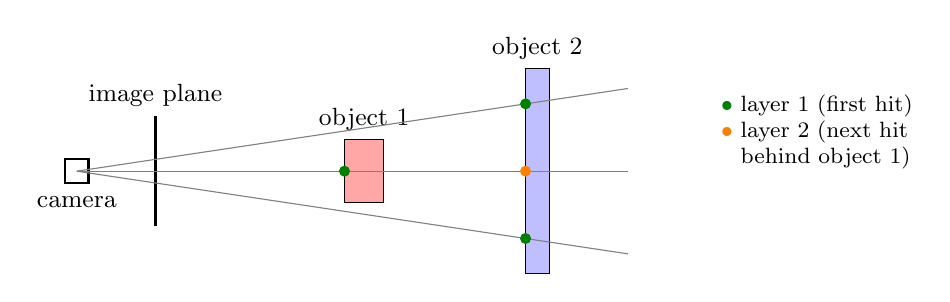
\begin{tikzpicture}[font=\small]
\draw[thick] (-0.15,-0.15) rectangle (0.15,0.15); \node[below] at (0,-0.2) {camera};
\draw[thick] (1,-0.7) -- (1,0.7); \node[above] at (1,0.7) {image plane};
\draw[fill=red!35] (3.4,-0.4) rectangle (3.9,0.4); \node[above] at (3.65,0.4) {object 1};
\draw[fill=blue!25] (5.7,-1.3) rectangle (6.0,1.3); \node[above] at (5.85,1.3) {object 2};
\foreach \s in {0.15,0,-0.15}{\draw[gray] (0,0) -- (7,7*\s);}
\fill[green!50!black] (5.7,0.855) circle (2pt);
\fill[green!50!black] (3.4,0) circle (2pt); \fill[orange] (5.7,0) circle (2pt);
\fill[green!50!black] (5.7,-0.855) circle (2pt);
\node[align=left,font=\footnotesize] at (9.4,0.5) {\textcolor{green!50!black}{$\bullet$} layer 1 (first hit)\\\textcolor{orange}{$\bullet$} layer 2 (next hit\\ \hphantom{$\bullet$} behind object 1)};
\end{tikzpicture}
\caption{Three pixel rays. The upper and lower rays hit only object 2 (layer 1 only); the middle ray hits object 1 first and object 2 second, so its pixel stores two (depth, colour) entries.}
\end{figure}

\begin{intuition}
A depth map keeps only the first hit along each ray; an LDI keeps a \emph{list} of hits. The hidden second layer (what is behind object 1) is what allows rendering from a slightly different viewpoint without holes; but the layer index jumps around from pixel to pixel, so layers are not smooth images.
\end{intuition}

\subsection{Multi-plane Images \slides{slide 70}}
Multi-plane images (MPIs) are discrete volumetric representations with \emph{non-uniform} spatial cells: a stack of fronto-parallel planes at fixed depths, each a (colour, transparency) image. They are extremely efficient to render (each layer is just a plane at fixed depth), but have limited resolution for far-away content; uniform cells may be preferable for object-centric 3D.

\begin{figure}[ht]
\centering
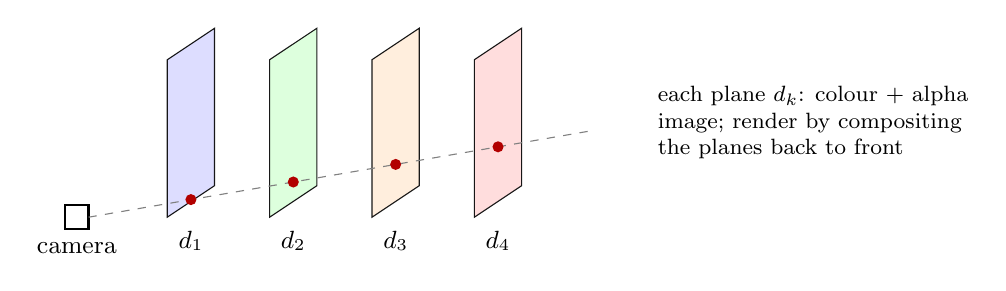
\begin{tikzpicture}[font=\small]
\foreach \k/\c in {0/blue!15,1/green!15,2/orange!15,3/red!15}{
  \draw[fill=\c,opacity=0.9] (\k*1.3,0)--(\k*1.3+0.6,0.4)--(\k*1.3+0.6,2.4)--(\k*1.3,2.0)--cycle;
  \node[below] at (\k*1.3+0.3,-0.05) {$d_{\the\numexpr\k+1\relax}$};
}
\draw[thick] (-1.3,-0.15) rectangle (-1.0,0.15); \node[below] at (-1.15,-0.2) {camera};
\draw[gray,dashed] (-1.0,0) -- (5.4,1.1);
\foreach \k in {0,1,2,3}{\fill[red!70!black] ({\k*1.3+0.3},{(\k*1.3+1.3)*0.1719}) circle (2pt);}
\node[align=left,font=\footnotesize] at (8.2,1.2) {each plane $d_k$: colour + alpha\\image; render by compositing\\the planes back to front};
\end{tikzpicture}
\caption{A multi-plane image: planes at increasing depth $d_1<\dots<d_4$; a pixel ray crosses all of them and the result is their composite.}
\end{figure}

\begin{intuition}
An MPI is a pile of transparent slides at fixed depths: to draw the scene from a nearby viewpoint, shift and blend the slides. Planes are spaced non-uniformly (dense near, sparse far), which is why distant content gets little resolution.
\end{intuition}

\subsection{CAD Models and CSG Trees \slides{slide 71}}
CAD models and CSG (constructive solid geometry) trees are \emph{compositions of primitive volumes or surfaces}. They are popular across design applications but challenging for learning.

\begin{figure}[ht]
\centering
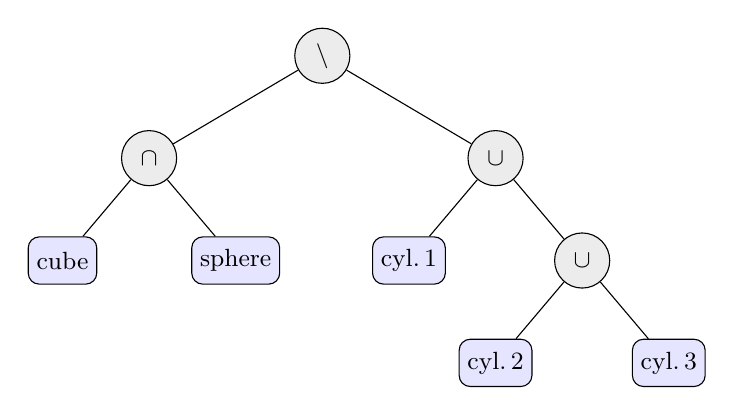
\begin{tikzpicture}[font=\small,
 op/.style={circle,draw,fill=gray!15,minimum size=7mm,inner sep=0pt},
 pr/.style={draw,rounded corners,fill=blue!10,minimum height=6mm,inner sep=3pt}]
\node[op] (r) at (0,0) {$\setminus$};
\node[op] (l) at (-2.2,-1.3) {$\cap$};
\node[op] (rr) at (2.2,-1.3) {$\cup$};
\node[pr] (c) at (-3.3,-2.6) {cube};
\node[pr] (s) at (-1.1,-2.6) {sphere};
\node[pr] (y1) at (1.1,-2.6) {cyl.\,1};
\node[op] (u) at (3.3,-2.6) {$\cup$};
\node[pr] (y2) at (2.2,-3.9) {cyl.\,2};
\node[pr] (y3) at (4.4,-3.9) {cyl.\,3};
\draw (r)--(l) (r)--(rr) (l)--(c) (l)--(s) (rr)--(y1) (rr)--(u) (u)--(y2) (u)--(y3);
\end{tikzpicture}
\caption{A CSG tree: leaves are primitives, inner nodes are Boolean operations (as on slide 71: $(\text{cube}\cap\text{sphere})\setminus(\text{cyl.}_1\cup(\text{cyl.}_2\cup\text{cyl.}_3))$).}
\end{figure}

\begin{example}[A CSG tree is a nested $\min/\max$]
If each primitive has an implicit function ($f_{\text{cube}},f_{\text{sph}},f_{c1},f_{c2},f_{c3}$), the tree of the figure is the field
\[
f=\max\Big(\max(f_{\text{cube}},f_{\text{sph}}),\;-\min\big(f_{c1},\min(f_{c2},f_{c3})\big)\Big),
\]
by the Boolean rules of slide 52.
\end{example}

\begin{intuition}
A CSG model is a \emph{program}: a recipe of primitives and Boolean steps. It is compact, editable and exact, but the structure (which tree, how deep) is discrete and combinatorial, so it is hard to predict with a neural network by gradient descent.
\end{intuition}

% =====================================================================
\section{Summary \slides{slides 72--74}}\label{sec:summary}
% =====================================================================

The summary slide (72) repeats the zoo of slide 4: mesh, point cloud, CAD model, voxels, implicit surface $\{\vx\mid f(\vx)=0\}$, parametric surface $f(\vu)=\vx\in\R^3$, CSG tree, and many more. Slides 73--74 are ``Questions?'' and Acknowledgments: the slides are adapted from \emph{Learning for 3D Vision}, CMU 16-825, Prof.\ Shubham Tulsiani.

\subsection*{Comparison table}
\newcommand{\Y}{\cellcolor{green!25}}
\newcommand{\Pm}{\cellcolor{yellow!30}}
\newcommand{\N}{\cellcolor{red!22}}
\begin{center}
\small
\renewcommand{\arraystretch}{1.3}
\setlength{\tabcolsep}{3pt}\begin{tabular}{L{2.3cm}L{2.3cm}L{2.3cm}L{2.5cm}L{2.3cm}L{2.3cm}}
\toprule
 & \textbf{Get surface points} & \textbf{Inside / outside} & \textbf{Change topology continuously} & \textbf{Render directly} & \textbf{Memory scales with}\\
\midrule
Point cloud & \Y given & \N no surface & \Y any point set & \Pm splats & points ($N$)\\
Triangle mesh & \Y sample triangles & \Pm count ray crossings & \N same wiring only & \Y rasterizer & vertices, faces\\
Parametric & \Y evaluate $f$ & \N search over $\vu$ & \N same topology only & \N via a mesh & parameters of $f$\\
Voxels & \Pm marching cubes & \Y look up cell & \Pm with probabilities & \Pm blocky & $n^3$\\
Implicit / SDF & \Pm marching cubes & \Y sign of $f$ & \Y any topology & \Pm ray marching & grid $n^3$ or network\\
\bottomrule
\end{tabular}
\end{center}
{\noindent\footnotesize \colorbox{green!25}{\strut easy}\quad\colorbox{yellow!30}{\strut possible with effort}\quad\colorbox{red!22}{\strut hard / limited}. Ratings are our reading of slides 22--62 and the table of slide 66, not a table from the slides.}

\begin{figure}[ht]
\centering
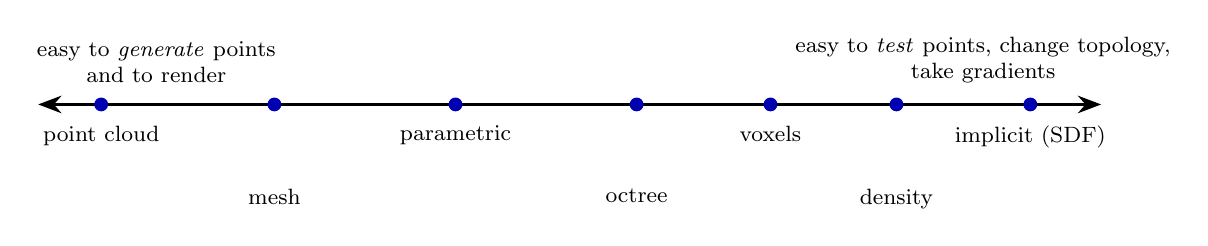
\begin{tikzpicture}[font=\small,>=Stealth]
\draw[<->,very thick] (0,0)--(13.5,0);
\node[above,align=center,font=\footnotesize] at (1.5,0.15) {easy to \emph{generate} points\\and to render};
\node[above,align=center,font=\footnotesize] at (12,0.15) {easy to \emph{test} points, change topology,\\take gradients};
\foreach \x/\t/\y in {0.8/point cloud/-0.6,3.0/mesh/-1.4,5.3/parametric/-0.6,7.6/octree/-1.4,9.3/voxels/-0.6,10.9/density/-1.4,12.6/implicit (SDF)/-0.6}{
  \fill[blue!70!black] (\x,0) circle (2.5pt); \node[below] at (\x,\y+0.45) {\footnotesize\t};
}
\end{tikzpicture}
\caption{A qualitative map of the ``generate vs.\ test'' spectrum (our summary of slides 41, 48, 62 and 66; positions are indicative only).}
\end{figure}

\subsection*{Key take-aways}
\begin{itemize}
\item \textbf{There is no universal 3D representation.} Points and depth maps come from sensors; meshes are for rendering and graphics; implicit fields are for inside/outside tests, topology changes and learning; the right choice depends on the task.
\item \textbf{Parametric generates, implicit tests.} $f(\vu)=\vx$ makes sampling trivial and queries hard; $\{f(\vx)=0\}$ makes queries trivial (sign of $f$, $\nabla f$ for normals, $\min/\max$ for Booleans) and sampling hard.
\item \textbf{Meshes split geometry from connectivity.} $V$ is continuous and optimizable; $F$ is discrete, so predicting arbitrary connectivity or changing topology is hard; check winding order, and remember $F\approx2V$ for closed genus-0 meshes.
\item \textbf{Grids are simple but pay for empty space.} A $n^3$ voxel grid (or SDF grid) handles any topology and suits convolutions, but only $\sim n^2$ cells touch the surface; octrees and continuous fields (networks, Gaussians) fight this cost.
\item \textbf{SDFs are the well-behaved implicit fields.} $\norm{\nabla f}=1$ makes $|f|$ the true distance, enabling safe ray-marching steps and TSDF fusion, and marching cubes converts any such field back into a mesh.
\end{itemize}

% % =====================================================================
% \appendix
% \section{Appendix: Harmonic Functions and the Winding Number \slides{slide 75, backup slide}}\label{app:winding}
% % =====================================================================
% \emph{Supplementary: this slide appears in the file \textbf{after} the Questions and Acknowledgments slides (it is a backup slide), so it is kept out of the main flow.}

% Slide 75 presents the winding number as an alternative implicit function:
% \begin{definition}[Winding number]
% $w(\vx)$ is the signed solid angle of $\Surf$ seen from $\vx$, divided by $4\pi$. On the slide: $w=1$ inside, $w=0$ outside, and the surface sits at $w=\tfrac12$; $w$ is harmonic \emph{away from} the surface; it is robust (holes and noise give fractional values); and it is defined even for an oriented point cloud, which is why reconstruction uses it (slide credits: Barill et al.\ 2018, Gillespie et al.\ 2024, Chen et al.\ 2024).
% \end{definition}

% For a closed surface with outward normals the standard integral form (not written on the slide) is $w(\vx)=\frac1{4\pi}\int_{\Surf}\frac{(\vy-\vx)\cdot\vn(\vy)}{\norm{\vy-\vx}^3}\,dA(\vy)$.

% \begin{figure}[ht]
% \centering
% \begin{tikzpicture}
% \begin{axis}[width=0.75\linewidth,height=5cm,xlabel={position along a line through the unit disk (2D analogue)},ylabel={$w$},xmin=-2,xmax=2,ymin=-0.1,ymax=1.15,ytick={0,0.5,1},grid=both]
% \addplot[thick,blue,const plot] coordinates {(-2,0)(-1,0)(-1,1)(1,1)(1,0)(2,0)};
% \addplot[only marks,mark=*,red] coordinates {(-1,0.5)(1,0.5)};
% \end{axis}
% \end{tikzpicture}
% \caption{2D analogue: $w$ is the angle subtended by the curve divided by $2\pi$. It is $1$ inside, $0$ outside, and exactly $\tfrac12$ on the curve (red dots), where the curve fills half of the viewing directions.}
% \end{figure}

% \begin{intuition}
% Stand at $\vx$ and ask ``what fraction of my full view sphere is covered by the surface, counting front-side coverage positively?'': inside a closed shape you see it all around you (fraction $1$), outside it is cancelled out (front and back cancel, fraction $0$), and standing \emph{on} the surface you are covered on one half (fraction $\tfrac12$). If the surface has a small hole or noise, a point just inside sees slightly less than everything, giving a value like $0.95$ rather than a hard failure. That graceful behaviour makes $w$ useful for turning oriented point clouds into implicit surfaces.
% \end{intuition}

\newpage

% ======================================================================
% Lecture 3
% ======================================================================
\part{Lecture 3}

\begin{tcolorbox}[colback=gray!6,colframe=gray!60,boxrule=0.5pt,arc=2pt]
\textbf{How to read these notes.} Section headers reuse the titles of the slides and are tagged with the slide range they cover. Formal statements (definitions, propositions, theorems, algorithms) are placed where the slides introduce the topic; the slides themselves state most results without proof, so the derivations are added here. Blue \emph{Intuition} boxes explain the ``why'' in plain words, with worked numbers. All figures are original TikZ/pgfplots drawings; figures marked \emph{schematic} show the qualitative trend described on the slides, not measured data.
\end{tcolorbox}

\begingroup
\sloppy

\endgroup
\newpage
% =====================================================================
\section{From Image Formation to Measurement \slides{1--3}}
% =====================================================================
Lecture 01 modeled how a scene becomes an image: projection sends a 3D point to a pixel and \emph{discards the distance along the ray}. Lecture 02 covered ways to \emph{represent} a scene: points, meshes, voxels, signed distance functions, Gaussians. Neither lecture covered how to \emph{measure} a scene. This lecture obtains one depth value per pixel (not always -- some sensors leave holes) in one of three ways: by measuring it with a laser, by stereo vision, or by \emph{predicting} it with a learned prior.
 

\begin{figure}[H]
	\centering
	\includegraphics[width=1.0\linewidth]{1790767754174.png}
\end{figure}

\begin{table}[htbp]
\centering\small
\begin{tabular}{llc}
\toprule
Section & Title & Slides\\
\midrule
3.1 & From representations to measurements & 4--7\\
3.2 & Three ways to pay for depth & 8--12\\
3.3 & Inside a LiDAR & 13--17\\
3.4 & From point cloud to depth image & 18--19\\
3.5 & From recovery to prediction & 20--22\\
3.6 & Cues in closed form & 23--26\\
3.7 & Supervised single-view depth & 27--35\\
3.8 & Cues used by the network & 36--39\\
\bottomrule
\end{tabular}
\caption{The agenda (slide 3) with slide ranges.}
\end{table}
 
\begin{intuition}
The whole lecture is one story: an image is a \emph{projection}, so depth is missing. Every method for getting it back must \emph{pay} with something -- time (a laser pulse), a baseline (a second viewpoint), computation (motion), or a prior (assumptions learned from data). The interesting questions are always: what did we pay, and what is therefore \emph{guaranteed} about the answer?
\end{intuition}
 
% =====================================================================
\section{From Representations to Measurements \slides{4--7}}
% =====================================================================
\emph{What one image determines, and what it does not.} The two preceding lectures modeled image formation and scene representation. This section separates \emph{recovered} from \emph{ambiguous} quantities and shows which of the two depth from one image is.
 
\subsection{Recovered and Ambiguous Quantities \slides{5}}
 
\begin{definition}[Recovered vs.\ ambiguous quantity]
Every quantity estimated in this lecture falls into one of two cases.
\begin{itemize}
\item \textbf{Recovered}: the data determine it up to noise. It can be reported in meters with an error bar.
\item \textbf{Ambiguous}: the data determine it only up to a \emph{family of transformations}. Any single number reported for it comes from an added assumption.
\end{itemize}
\end{definition}
 
\begin{table}[htbp]
\centering\small
\begin{tabular}{lcp{5.6cm}}
\toprule
Quantity & Free parameters & What pins it down\\
\midrule
metric depth & $0$ & nothing, it is already in meters\\
up to scale & $1$ ($s$) & one known length\\
up to scale and shift & $2$ ($s,t$) & two known depths\\
ordering only & any monotone map & a calibrated sensor\\
\bottomrule
\end{tabular}
\caption{Ambiguity ladder (slide 5). The number of free parameters says how much external information is still needed.}
\end{table}
 
\begin{intuition}
Think of the free parameters as \emph{knobs you cannot read from the data}. Metric depth has no knob. ``Up to scale'' has one knob: the scene may be uniformly inflated or shrunk. ``Up to scale and shift'' has two. ``Ordering only'' is the weakest: you know that $A$ is nearer than $B$, but $(1,2,3)$ and $(1,10,100)$ tell exactly the same story. The slide's punchline: disagreements about depth estimation are usually disagreements about \emph{which row of this table a quantity lives in}.
\end{intuition}
 
\subsection{The Back-Projected Ray \slides{6}}
 
Projection throws one number away per pixel; inverting it asks for that number back:
\begin{equation}\label{eq:backproj}
\bm p^{c} \;=\; z\,\Kinv\,\xt_s .
\end{equation}
Here $\xt_s$ is the homogeneous pixel (third component $1$), $\bm K$ the intrinsics from lecture 01, and $\bm p^c$ the point in the camera frame.
 
\begin{proposition}[Projection is not invertible]\label{prop:ray}
The third component of $\Kinv\xt_s$ is $1$, so the free scalar $z$ in \eqref{eq:backproj} is the depth in meters along the optical axis. Given only $\bm x_s$, the set of 3D points that project to it is the whole ray
\[
\{\, z\,\Kinv\xt_s \;:\; z>0 \,\}.
\]
\end{proposition}
\begin{proof}
Third row of $\bm K$ is $(0,0,1)$, hence $\bm K\bm p^c=(\ast,\ast,p^c_z)^\top$ and $\bm p^c$ projects to $\xt_s$ iff $\bm K\bm p^c=\lambda\xt_s$ with $\lambda=p^c_z$ (homogeneous division). Solving, $\bm p^c=\lambda\Kinv\xt_s$ and $\lambda=z$. Conversely every $z\Kinv\xt_s$ satisfies $\bm K(z\Kinv\xt_s)=z\xt_s\sim\xt_s$. \qedhere
\end{proof}
 
\begin{figure}[htbp]
\centering
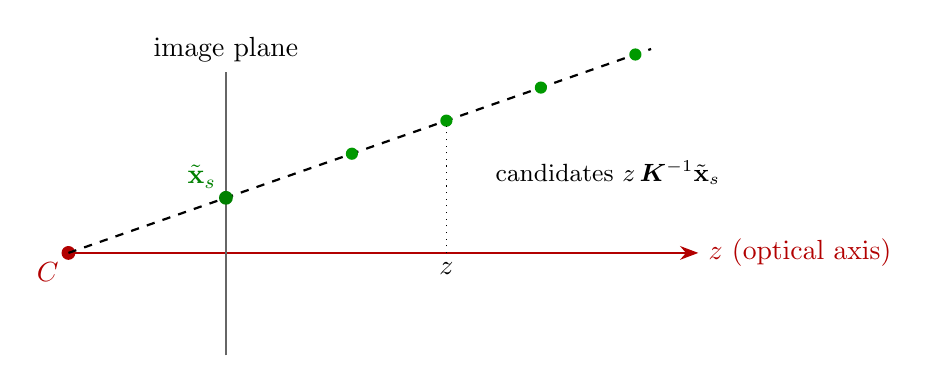
\begin{tikzpicture}[>=Stealth]
\draw[->,thick,red!70!black] (0,0)--(8,0) node[right]{$z$ (optical axis)};
\draw[thick,black!60] (2,-1.3)--(2,2.3) node[above,black]{image plane};
\fill[red!70!black] (0,0) circle(2.5pt) node[below left]{$C$};
\draw[dashed,thick] (0,0)--(7.4,2.59);
\fill[green!50!black] (2,0.7) circle(2.5pt) node[above left]{$\xt_s$};
\foreach \zz in {3.6,4.8,6.0,7.2} \fill[green!60!black] (\zz,{0.35*\zz}) circle(2.2pt);
\draw[dotted] (4.8,0)--(4.8,1.68);
\node[below] at (4.8,0) {$z$};
\node[anchor=north west] at (5.3,1.3) {\small candidates $z\,\Kinv\xt_s$};
\end{tikzpicture}
\caption{Back-projected ray (redrawn from slide 6; side view, $y$ up). Every green point projects to the same pixel.}\label{fig:ray}
\end{figure}
 
\begin{intuition}
It is like knowing the \emph{direction} in which a laser pointer is aimed but not how far away the dot lands. The information was \emph{destroyed at capture}, not merely hidden: no clever algorithm can un-destroy it, so every method that produces $z$ is either measuring something extra or importing an assumption. ``Producing $z$ at every pixel is the whole of this lecture.''
\end{intuition}
 
\subsection{Scale-Depth Ambiguity \slides{7}}
 
\begin{proposition}[Global scale is unobservable from one image]\label{prop:scale}
Let $\{\bm p_j\}$ be a scene in the camera frame and $s>0$. The scaled scene $\{s\bm p_j\}$ produces exactly the same image.
\end{proposition}
\begin{proof}
$\pi(\bm K\,s\bm p)=\pi(s\,\bm K\bm p)=\pi(\bm K\bm p)$, because the homogeneous division cancels $s$. \qedhere
\end{proof}
 
\begin{figure}[htbp]
\centering
\begin{tikzpicture}[>=Stealth]
\fill[blue!60!black] (0,0) circle(2pt) node[left]{eye};
\draw[dashed,blue!60!black] (0,0)--(8,1.6);
\draw[dashed,blue!60!black] (0,0)--(8,-1.6);
\draw[thick,black!60] (1.5,-0.3)--(1.5,0.3) node[above]{\scriptsize image};
\draw[very thick,red!70!black] (3,-0.6)--(3,0.6) node[above]{\scriptsize small, near};
\draw[very thick,red!70!black] (6,-1.2)--(6,1.2) node[above]{\scriptsize large, far};
\end{tikzpicture}
\caption{Scale-depth ambiguity (schematic after slide 7): a small near object and an object twice as large at twice the distance subtend the same angle.}
\end{figure}
 
\begin{figure}[H]
	\centering
	\includegraphics[width=1.0\linewidth]{1790767924564.png}
	\caption{two photos of a giant red bench, the second with a bicycle placed on it}\label{fig:1790767924564}
\end{figure}
 
\begin{intuition}
A small close object looks the same as a much larger one further away. The giant bench in the slide's photographs is a real-life example: on its own it reads as a normal bench, and only the bicycle on top reveals its true size. That bicycle is exactly a \emph{prior about sizes} -- the theme of the rest of the lecture.
\end{intuition}
 
% =====================================================================
\section{Three Ways to Pay for Depth \slides{8--12}}
% =====================================================================
\emph{Time, a baseline, a prior.} No method returns depth for free. Each buys it with a different resource, and the resource decides what the result is good for.
 
\subsection{Two Measurement Principles \slides{9}}
 
\begin{definition}[Time of flight and triangulation]
Two independent choices: the \emph{principle} decides what is measured; the \emph{illumination} decides only whether the sensor brings its own light (\emph{active}) or uses ambient light (\emph{passive}).
\begin{itemize}
\item \textbf{Time of flight (ToF)}: measure the delay of emitted light.
\item \textbf{Triangulation}: measure the angular/pixel difference between two viewpoints separated by a known geometry.
\end{itemize}
\end{definition}
 
\begin{table}[htbp]
\centering\small
\sloppy
\hbadness=10000
\begin{tabularx}{\linewidth}{@{}p{3.1cm}YY@{}}
\toprule
 & time of flight & triangulation\\
\midrule
\textbf{active} (own light) & scanning laser, flash range camera & projected-pattern camera, active stereo\\
\textbf{passive} (ambient light) & \emph{empty}: timing needs a known emission & stereo with a known baseline, structure from motion\\
\bottomrule
\end{tabularx}
\caption{The two-by-two of depth sensing (slide 9).}
\end{table}
 
 
\begin{figure}[H]
	\centering
	\includegraphics[width=1.0\linewidth]{1790767988279.png}
	\caption{left: speckle pattern of a projected-pattern camera with a stereo camera overlaid; right: a Hesai spinning LiDAR}\label{fig:1790767988279}
\end{figure}

\begin{intuition}
The empty cell is instructive: to time light you must \emph{know when it left}, and ambient light has no known departure time. Also, ``active'' only helps with texture or timing -- it does not change the physics: a projected pattern camera is still triangulation, it just paints texture onto blank walls so matching works.
\end{intuition}
 
\subsection{Triangulation From Two Views \slides{10}}
 
Two rectified cameras sit a baseline $b$ apart. A scene point $\bm p=(x,y,z)\in\R^3$ appears at horizontal pixel offsets $u_L$ and $u_R$ (relative to each principal point), and similar triangles give the depth.
 
\begin{theorem}[Depth from disparity]\label{thm:stereo}
For two rectified cameras with focal length $f$ (in pixels) and baseline $b$ (in meters), the depth of a point with disparity $d=u_L-u_R$ is
\[
z=\frac{f\,b}{d}.
\]
\end{theorem}
\begin{proof}
By the pinhole model $u_L=f\,x/z$ for the left camera, and since the right camera is displaced by $b$ along $x$, $u_R=f\,(x-b)/z$. Subtracting, $d=u_L-u_R=fb/z$. (The slide draws the image plane behind the pinhole, which produces the minus signs in its two similar-triangle equations; the resulting formula is the same.) \qedhere
\end{proof}
 
\begin{figure}[htbp]
\centering
\begin{tikzpicture}[>=Stealth,scale=1.1]
\fill (0,0) circle(2pt) node[below]{$C_L$};
\fill (3,0) circle(2pt) node[below]{$C_R$};
\draw[<->,orange!80!black] (0,-0.6)--(3,-0.6) node[midway,below]{$b$};
\draw[thick,black!60] (-0.9,1)--(0.9,1);
\draw[thick,black!60] (2.1,1)--(3.9,1);
\draw[dashed,gray] (0,0)--(0,1.5);
\draw[dashed,gray] (3,0)--(3,1.5);
\fill[blue!60!black] (1.6,4) circle(2.5pt) node[above]{$\bm p=(x,y,z)$};
\draw (0,0)--(1.6,4);
\draw (3,0)--(1.6,4);
\fill[red!70!black] (0.4,1) circle(1.8pt);
\fill[red!70!black] (2.65,1) circle(1.8pt);
\node[red!70!black,above] at (0.2,1.02) {\scriptsize $u_L$};
\node[red!70!black,above] at (2.82,1.02) {\scriptsize $u_R$};
\draw[<->] (-1.3,0)--(-1.3,1) node[midway,left]{$f$};
\draw[<->,gray] (4.4,0)--(4.4,4) node[midway,right]{$z$};
\end{tikzpicture}
\caption{Rectified stereo (redrawn from slide 10, top view). With $f=1$, $b=3$, $z=4$ as drawn: $u_L=0.4$, $u_R=-0.35$, $d=0.75=fb/z$.}
\end{figure}
 
\begin{corollary}[Unknown baseline]\label{cor:unknownb}
Disparity is inverse depth scaled by $fb$: $1/z=d/(fb)$. If $b$ is unknown (a moving camera), depth is known only up to one global scale.
\end{corollary}
 
\begin{example}
For $f=700$\,px and $b=0.5$\,m, $fb=350$ px\,m and $z=350/d$: $d=70$\,px means $5$\,m, $d=17.5$\,px means $20$\,m, $d=7$\,px means $50$\,m.
\end{example}
 
\begin{intuition}
\textbf{Where meters come from:} $b$ is in meters, so $z$ is in meters -- the baseline is the source of scale. Hold a finger at arm's length and blink one eye at a time: the finger jumps a lot against the background; a distant tree barely moves. That jump \emph{is} the disparity, and it is large for near things (large $1/z$). \textbf{Matching} is the price: $d$ requires finding the \emph{same} point in both images, which fails on textureless or repetitive surfaces and wherever a surface is visible to one view only. Because disparity is $fb$ times inverse depth, an unknown rig only leaves an unknown \emph{scale} in disparity, which is why affine invariance in \emph{disparity} suits data whose rig is unknown (used in \S3.7).
\end{intuition}
 
\subsection{The Three Currencies \slides{11}}
 
\begin{table}[htbp]
\centering\small
\begin{tabularx}{\linewidth}{@{}p{2.2cm}YYY@{}}
\toprule
pay with & method & gives & costs\\
\midrule
\textbf{time} & emit a pulse and time the return (LiDAR) & metric depth, directly & sparse, expensive, returns missing\\
\textbf{a baseline} & stereo, baseline known & metric depth, dense where matching works & a calibrated second camera; error growing as $z^2$\\
\textbf{computation} & structure from motion, baseline unknown & shape up to one global scale & a moving camera and a rigid scene\\
\textbf{a prior} & assumptions learned from data & dense, from one image, cheap & not metric, and only as good as the prior\\
\bottomrule
\end{tabularx}
\caption{The three currencies (slide 11).}
\end{table}
 
\subsection{The Single-Image Claim \slides{12}}
 
The usual motivation for single-image depth is that it bypasses \emph{all} these limitations. The slide's verdict: a single image does bypass the \textbf{cost}, the \textbf{sparsity} and the \textbf{hardware}, but it cannot bypass the \textbf{physics}, because it \emph{never measured anything}. The result is therefore an \emph{ambiguous} quantity (same ray picture as Figure~\ref{fig:ray}).
 
\begin{intuition}
Single-image depth is not a cheaper LiDAR; it is a different kind of object. It converts the question ``how far?'' into ``how far, \emph{given how scenes usually look}?'' -- a guess with an informed prior. Keeping this distinction in mind explains every failure mode in \S3.8.
\end{intuition}
 
% =====================================================================
\section{Inside a LiDAR \slides{13--17}}
% =====================================================================
\emph{Paying with time.} Outdoor depth labels are produced by a scanning laser, and their error sources are inherited by any network trained on them -- so we need to know how a LiDAR fails.
 
\subsection{Pulsed Time of Flight \slides{14}}
 
A short pulse is emitted and a clock runs until the echo returns. The light covers the distance twice, so the interval is halved:
\begin{equation}\label{eq:tof}
r=\frac{c\,t}{2}.
\end{equation}
Each beam leaves in a known direction, so a return is a \emph{direction plus a range}; the energy that comes back is reported as \emph{intensity}. Pulse widths are a few nanoseconds (typically 5--10\,ns, about 4\,ns in modern full-waveform scanners). Every other part of the sensor exists to make the interval $t$ reliable.
 
\begin{example}
An echo from $50$\,m returns after $t=2\cdot 50/(3\cdot10^8)\approx 333$\,ns. A timing error of $1$\,ns corresponds to $c\,\delta t/2\approx 15$\,cm of range. A $5$\,ns pulse is $c\cdot 5\,\text{ns}\approx1.5$\,m long in space.
\end{example}
 
\begin{intuition}
It is echolocation with light: shout and time the echo. The factor $\tfrac12$ is just the round trip. Because $c$ is so large, centimeter accuracy demands sub-nanosecond timing -- which is why timing electronics dominate the design.
\end{intuition}
 
\subsection{Structured Sparsity \slides{15}}
 
Azimuth resolution is set by the spin rate; elevation resolution is fixed in hardware. The two differ, so the sampling is \emph{anisotropic}.
 
\begin{definition}[Scan-line spacing]
For a vertical angular pitch $\Delta\theta_{\text{el}}$ (radians), the spacing between adjacent scan lines at range $r$ is
\[
s(r)\approx r\,\Delta\theta_{\text{el}}.
\]
\end{definition}
 
\begin{example}[Velodyne VLP-16]
At $5$\,Hz the sensor samples every $0.1^\circ$ in azimuth; at $20$\,Hz every $0.4^\circ$ -- spinning faster costs horizontal resolution. Vertically it is stuck at $\Delta\theta_{\text{el}}=2.0^\circ=0.0349$\,rad, so the scan lines are $0.70$\,m apart at $20$\,m and $1.75$\,m apart at $50$\,m. A pedestrian at $50$\,m is crossed by one scan line or by none. (For comparison, the azimuth gap at $50$\,m is only $0.09$\,m at $5$\,Hz and $0.35$\,m at $20$\,Hz.)
\end{example}
 
\begin{figure}[htbp]
\centering
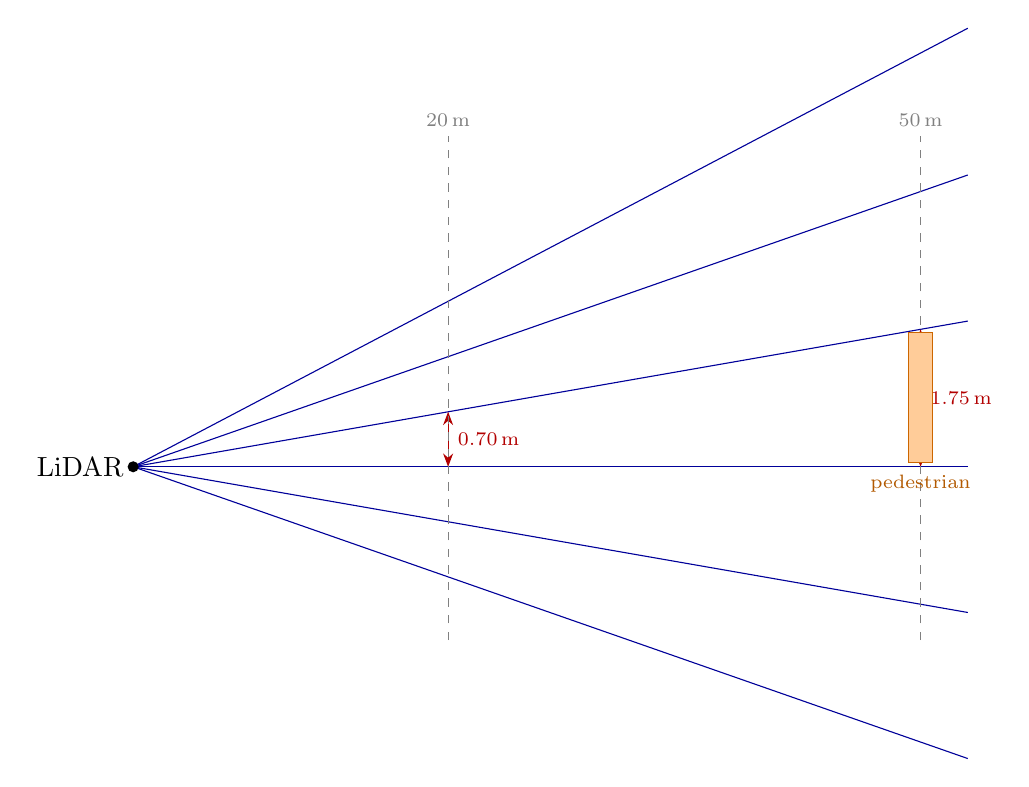
\begin{tikzpicture}[>=Stealth,x=1cm,y=1cm]
% horizontal: 1 cm = 5 m ; vertical: 1 cm = 1 m  (exaggerated vertically)
\foreach \k in {-2,-1,0,1,2,3}{
  \draw[blue!60!black] (0,0)--(10.6,{5*tan(2*\k)*10.6});
}
\fill (0,0) circle(2pt) node[left]{LiDAR};
\draw[<->,red!70!black] (4,0)--(4,{5*tan(2)*4}) node[midway,right]{\scriptsize $0.70$\,m};
\draw[<->,red!70!black] (10,0)--(10,{5*tan(2)*10}) node[midway,right]{\scriptsize $1.75$\,m};
\draw[dashed,gray] (4,-2.2)--(4,4.2) node[above]{\scriptsize $20$\,m};
\draw[dashed,gray] (10,-2.2)--(10,4.2) node[above]{\scriptsize $50$\,m};
% pedestrian, 1.7 m tall, between two rays at 50 m
\draw[fill=orange!40,draw=orange!80!black] (9.85,0.06) rectangle (10.15,1.70);
\node[orange!70!black,below] at (10,0.02) {\scriptsize pedestrian};
\end{tikzpicture}
\caption{Original figure (not on the slides): VLP-16 elevation fan with a $2^\circ$ pitch, side view. Vertical axis exaggerated: $1$\,cm~=~$1$\,m vertically but $1$\,cm~=~$5$\,m along range. At $50$\,m a $1.7$\,m pedestrian fits between two consecutive scan lines and is missed.}
\end{figure}
 

\begin{figure}[H]
	\centering
	\includegraphics[width=1.0\linewidth]{1790768067024.png}
	\caption{colored LiDAR point cloud of a parking lot: concentric ring-like scan lines with gaps between them}\label{fig:1790768067024}
\end{figure}
 
\begin{intuition}
Picture the grooves of a vinyl record. Samples are dense \emph{along} a groove (azimuth) but grooves are far apart (elevation). Moving away from the sensor, the grooves spread linearly with range, while points along a groove stay comparatively tight. So a point cloud thins with distance along \emph{one axis} much faster than the other, and the gaps form horizontal stripes.
\end{intuition}
 
\subsection{Limitations of a LiDAR Point Cloud \slides{16}}
 
\begin{itemize}
\item \textbf{No color and no semantics.}
\item \textbf{No measurement where there was no return}, which is \emph{distinct from a zero depth}: ``I saw nothing'' is not ``the surface is at distance $0$''.
\item \textbf{No sample between scan lines}, and that gap grows linearly with range.
\item \textbf{Points that lie on no surface}: where one pulse straddles a silhouette, the echo mixes foreground and background into a single (wrong) range.
\end{itemize}
 
\begin{intuition}
The last item is the LiDAR analogue of an out-of-focus edge: half the beam hits the near object, half the far wall, and the reported range is somewhere in the empty air between them. Such ``flying'' points are a systematic error that a network trained on LiDAR labels will inherit at every object boundary.
\end{intuition}
 
\subsection{Two Error Laws \slides{17}}
 
The two principles fail in different ways, and the difference decides where each is worth using.
\[
\text{time of flight: }\ \delta r=\frac{c\,\delta t}{2},
\qquad
\text{triangulation: }\ \delta z\approx\frac{z^{2}\,\delta d}{f\,b}.
\]
 
\begin{proposition}[Triangulation error law]\label{prop:errlaw}
A disparity error $\delta d$ produces a depth error $\delta z\approx z^2\delta d/(fb)$: quadratic in range, even for a perfect sensor.
\end{proposition}
\begin{proof}
From Theorem~\ref{thm:stereo}, $z=fb/d$, so $\left|\frac{dz}{dd}\right|=\frac{fb}{d^2}=\frac{z^2}{fb}$. Multiply by $\delta d$. \qedhere
\end{proof}
 
The timing floor $c\,\delta t/2$ is \emph{independent of range}. What degrades with range is the \emph{precision}: the returned power falls as $1/r^2$ or $1/r^4$ (depending on whether the target is extended or smaller than the beam -- standard radar/LiDAR-equation background), and a weaker return is timed less precisely.
 
\begin{example}[Numbers from the slide]
With $f=700$\,px, $b=0.5$\,m and quarter-pixel matching ($\delta d=0.25$\,px), $fb=350$ and
\[
\delta z(5\,\text{m})=\tfrac{25\cdot0.25}{350}\approx 2\,\text{cm},\quad
\delta z(20\,\text{m})\approx 29\,\text{cm},\quad
\delta z(50\,\text{m})\approx 1.8\,\text{m}.
\]
The laser is exact where it lands, but at $50$\,m its scan lines are $1.75$\,m apart, so a pedestrian is crossed at most once.
\end{example}
 
\begin{figure}[htbp]
\centering
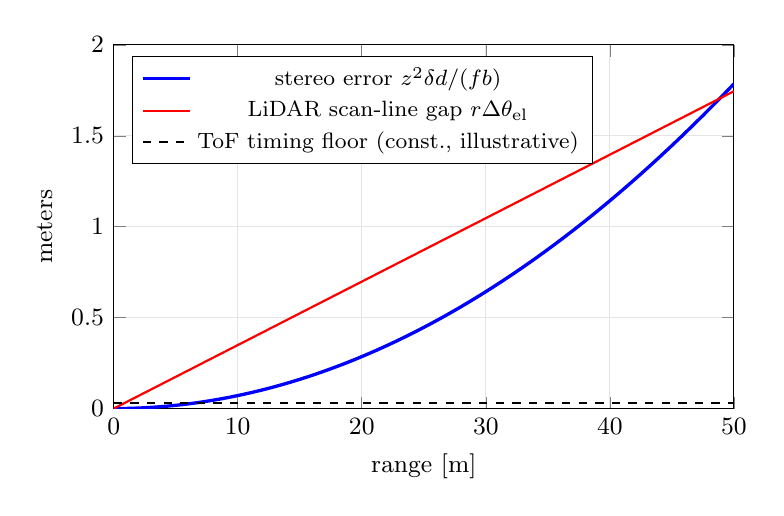
\begin{tikzpicture}
\begin{axis}[width=0.78\linewidth,height=6.2cm,xlabel={range [m]},ylabel={meters},xmin=0,xmax=50,ymin=0,ymax=2,
  legend style={at={(0.03,0.97)},anchor=north west,font=\footnotesize},grid=both,grid style={gray!20}]
\addplot[blue,very thick,domain=0:50,samples=60]{x^2*0.25/350};
\addlegendentry{stereo error $z^2\delta d/(fb)$}
\addplot[red,thick,domain=0:50,samples=2]{0.0349066*x};
\addlegendentry{LiDAR scan-line gap $r\Delta\theta_{\mathrm{el}}$}
\addplot[black,dashed,thick,domain=0:50,samples=2]{0.03};
\addlegendentry{ToF timing floor (const., illustrative)}
\end{axis}
\end{tikzpicture}
\caption{Original figure (not on the slides), from the slide's numbers: $f=700$\,px, $b=0.5$\,m, $\delta d=0.25$\,px, $\Delta\theta_{\text{el}}=2^\circ$. The ToF floor level ($3$\,cm) is only illustrative.}
\end{figure}
 
\begin{intuition}
The two sensors are \emph{complementary}: LiDAR is precise where it samples but leaves holes; stereo samples everywhere but each sample degrades quadratically. This is why the remaining sections either \emph{fuse} the two or \emph{replace the laser with a prior}.
\end{intuition}
 
% =====================================================================
\section{From Point Cloud to Depth Image \slides{18--19}}
% =====================================================================
\emph{Paying with time: from cloud to depth map.} A LiDAR produces a point cloud. Converting it to a depth map needs the extrinsic calibration, the intrinsics (lecture 01), and a rule for resolving points that fall in the same pixel.
 
\subsection{Projecting a Cloud Into the Image \slides{19}}
 
The extrinsics are applied, followed by the projection from lecture 01:
\begin{equation}\label{eq:lidarproj}
\xt_s=\bm\pi\!\left(\bm K\,[\,\bm R_{cl}\mid\bm t_{cl}\,]\,\tilde{\bm p}^{\,l}\right),
\end{equation}
where $\bm\pi(\cdot)$ is the homogeneous division and $\bm p^l$ a point in the LiDAR frame.
 
\begin{definition}[Depth map]
The number written into the pixel is the $z$ component in the \emph{camera} frame. The array of them is the depth map $\bm D:\Omega\to\R_{>0}$,
\[
\bm D[\bm x_s]=\big(\bm R_{cl}\,\bm p^{l}+\bm t_{cl}\big)_z .
\]
\end{definition}
 
The slide stresses that this \emph{differs from the range the LiDAR measured}.
 
\begin{proposition}[Depth versus range]\label{prop:rangez}
If $\theta$ is the angle between the ray of pixel $\bm x_s$ and the optical axis, then $z=r\cos\theta$, where $r=\|\bm p^c\|$ is the range; equivalently $r=z\,\|\Kinv\xt_s\|\ge z$.
\end{proposition}
\begin{proof}
By \eqref{eq:backproj}, $\bm p^c=z\,\Kinv\xt_s$ with $\Kinv\xt_s=(a,b,1)^\top$; so $r=z\sqrt{a^2+b^2+1}$. The unit direction has $z$-component $1/\sqrt{a^2+b^2+1}=\cos\theta$. \qedhere
\end{proof}
 
\begin{example}
A return with range $r=20$\,m at $30^\circ$ off the optical axis is written as $z=20\cos30^\circ\approx17.3$\,m in the depth map.
\end{example}
 
\begin{figure}[htbp]
\centering
\begin{tikzpicture}[>=Stealth,scale=1]
% frames
\begin{scope}[shift={(0,2.2)}]
\draw[->,thick] (0,0)--(0,0.8); \draw[->,thick] (0,0)--(0.8,0);
\node[left] at (0,0.4) {\scriptsize LiDAR};
\end{scope}
\begin{scope}[shift={(0.7,0)}]
\draw[->,thick,orange!80!black] (0,0)--(0,0.8); \draw[->,thick,orange!80!black] (0,0)--(0.8,0);
\node[below,orange!80!black] at (0.3,-0.05) {\scriptsize camera};
\end{scope}
\fill (7,1.0) circle(3pt) node[right]{$\bm p$};
\draw[dashed,thick] (0,2.2)--(7,1.0);
\draw[dashed,thick,orange!80!black] (0.7,0)--(7,1.0);
\draw[->,gray,thick] (0.15,1.6) to[bend right=40] (0.55,0.5);
\node[gray] at (1.6,1.15) {$\mathbf T_{cl}$};
\end{tikzpicture}
\hfill
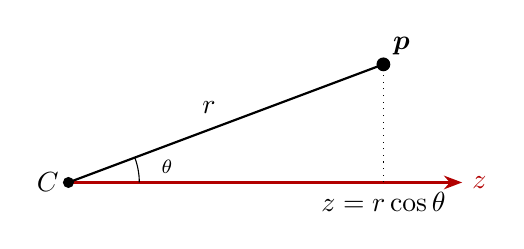
\begin{tikzpicture}[>=Stealth]
\draw[->,thick,red!70!black] (0,0)--(5,0) node[right]{$z$};
\fill (0,0) circle(2pt) node[left]{$C$};
\fill (4,1.5) circle(2.5pt) node[above right]{$\bm p$};
\draw[thick] (0,0)--(4,1.5) node[midway,above left]{$r$};
\draw[dotted] (4,0)--(4,1.5);
\node[below] at (4,0) {$z=r\cos\theta$};
\draw (0.9,0) arc(0:20.6:0.9); \node at (1.25,0.2) {\scriptsize $\theta$};
\end{tikzpicture}
\caption{Left: LiDAR and camera frames related by $\mathbf T_{cl}$ (redrawn from slide 19). Right: range $r$ versus depth $z$ (original figure).}
\end{figure}
 

\begin{figure}[H]
	\centering
	\includegraphics[width=1.0\linewidth]{1790768138707.png}
	\caption{grayscale image of a checkerboard target with LiDAR points projected onto it, colored by depth}\label{fig:1790768138707}
\end{figure}
 
\begin{algorithm}[LiDAR cloud to sparse depth map]
Input: points $\{\bm p^l_j\}$, intrinsics $\bm K$, extrinsics $(\bm R_{cl},\bm t_{cl})$, image size.
\begin{enumerate}[nosep]
\item Initialize $\bm D\leftarrow 0$ everywhere (``no measurement'').
\item For each point: $\bm p^c=\bm R_{cl}\bm p^l+\bm t_{cl}$; skip if $p^c_z\le0$ (behind the camera).
\item $\xt_s=\bm\pi(\bm K\bm p^c)$, round to a pixel; skip if outside the image.
\item If $\bm D[\bm x_s]=0$ or $p^c_z<\bm D[\bm x_s]$, set $\bm D[\bm x_s]\leftarrow p^c_z$.
\end{enumerate}
\end{algorithm}
 
\begin{intuition}
Step 4 is one common rule for ``points that fall in the same pixel'' (keep the nearest, as a z-buffer does); the slide only says such a rule is needed. Valid depths are strictly positive ($\bm D:\Omega\to\R_{>0}$), so $0$ can safely mark ``no return'' without colliding with a genuine measurement -- matching the earlier warning that a missing return is not a zero depth. Also remember that the result is \emph{sparse}: most pixels stay $0$.
\end{intuition}
 
% =====================================================================
\section{From Recovery to Prediction \slides{20--22}}
% =====================================================================
\emph{Paying with a prior.} One image does not determine depth. People judge it anyway, so they are supplying an assumption. This section turns that observation into a prior.
 
\subsection{Monocular Cues in Human Vision \slides{21}}
 
Not all 3D structures are equally likely, and human vision exploits that regularity through seven classic cues:
\begin{enumerate}[nosep]
\item linear perspective, \item relative size / position, \item texture gradient, \item occlusion (the occluded object is farther), \item aerial perspective, \item light and shadows, \item blur and defocus.
\end{enumerate}
 

\begin{figure}[H]
	\centering
	\includegraphics[width=1.0\linewidth]{1790768210811.png}
	\caption{driving image (highway scene) with the seven cues outlined and numbered}\label{fig:1790768210811}
\end{figure}
 
\begin{intuition}
None of these is a measurement. Each is an \emph{assumption about how scenes are usually arranged}: parallel lines meet, near things are big, far things are hazy. They work because the world is not a uniformly random set of 3D structures.
\end{intuition}
 
\subsection{Depth Prediction as a Prior \slides{22}}
 
\begin{proposition}[Bayesian view of single-image depth]\label{prop:bayes}
\[
p(\bm D\mid \bm I)\;\propto\; p(\bm I\mid \bm D)\,p(\bm D).
\]
The likelihood term is nearly flat along each ray (this is the ill-posedness of \S3.1), so the posterior is dominated by the prior $p(\bm D)$. Hence single-image depth is \emph{predicted} rather than \emph{recovered}, and a method is a claim about which scenes are likely.
\end{proposition}
 
\begin{intuition}
The likelihood asks: ``does this depth map explain the picture?'' Along a ray, every depth explains the pixel equally well, so the picture alone cannot vote. The only thing left to break ties is what depth maps \emph{usually look like} -- and people reading depth from a single photograph is everyday evidence that such a prior exists and is learnable. Where the learned one fails is the topic of \S3.8.
\end{intuition}
 
% =====================================================================
\section{Cues in Closed Form \slides{23--26}}
% =====================================================================
\emph{The prior, written in closed form.} Vanishing points, apparent size and vertical position each follow in one line from the projection equation.
 
\subsection{Vanishing Points \slides{24}}
 
Parallel 3D lines converge in the image; the horizon is the image of the line at infinity of the ground plane. A vanishing point is the image of a \emph{direction}, not of a location; every set of parallel lines has its own, and for a given plane they all lie on one line.
 
\begin{proposition}[Vanishing point of a direction]\label{prop:vp}
Let $\bm d\in\R^3$ be a 3D direction. Its image $\bm v$ satisfies
\[
\lambda\,\bm v=\bm K\,[\bm R\mid\bm t]\begin{pmatrix}\bm d\\0\end{pmatrix}=\bm K\bm R\,\bm d .
\]
\end{proposition}
\begin{proof}
A direction is a point at infinity, homogeneous coordinates $(\bm d,0)$. In the product $[\bm R\mid\bm t](\bm d,0)^\top=\bm R\bm d+\bm t\cdot0$ the translation is multiplied by zero and drops out. \qedhere
\end{proof}
 
\begin{corollary}
The horizon moves with camera \textbf{pitch and roll} only; translation does not move it.
\end{corollary}
 
\begin{example}[Horizon row for a pitched camera -- extra worked case]
Take zero roll, image $y$ pointing down, and pitch the camera up by $\theta$. The level forward direction has camera-frame coordinates $\bm R\bm d=(0,\sin\theta,\cos\theta)^\top$, so $\bm K\bm R\bm d$ gives the horizon row $y_h=c_y+f\tan\theta$: pitching up moves the horizon \emph{down} in the image.
\end{example}
 
\begin{figure}[htbp]
\centering
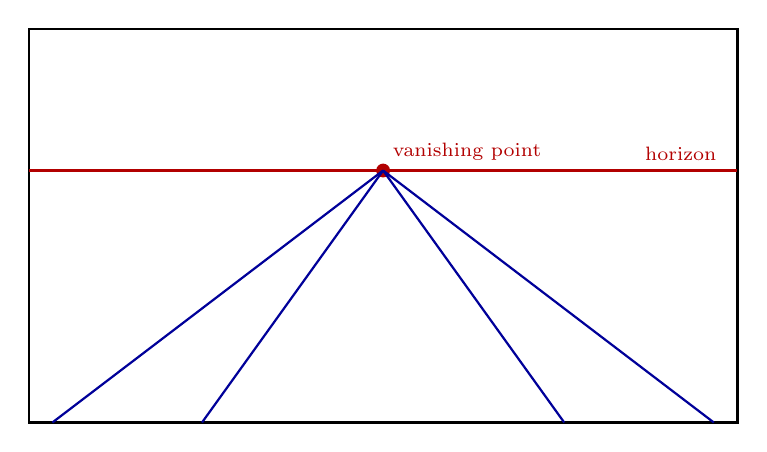
\begin{tikzpicture}[>=Stealth]
\draw[thick] (0,0) rectangle (9,5);
\draw[red!70!black,thick] (0,3.2)--(9,3.2) node[pos=0.92,above]{\scriptsize horizon};
\coordinate (V) at (4.5,3.2);
\fill[red!70!black] (V) circle(2.5pt) node[above right]{\scriptsize vanishing point};
\foreach \x in {0.3,2.2,6.8,8.7}{ \draw[blue!60!black,thick] (\x,0)--(V); }
\end{tikzpicture}
\caption{Original schematic (the slide shows a photograph, see below): parallel lines on the ground plane meet on the horizon.}
\end{figure}

 
\begin{figure}[H]
	\centering
	\includegraphics[width=1.0\linewidth]{1790768279993.png}
	\caption{photo of a wooden pier with yellow lines converging to a vanishing point on the horizon}\label{fig:1790768279993}
\end{figure}

\begin{intuition}
The translation drops out because a direction has no position: walking sideways does not change where the rails converge, only tilting the camera does. The slide adds a warning to remember: \emph{a network later on does not respect this} (\S3.8).
\end{intuition}
 
\subsection{Apparent Size \slides{25}}
 
\begin{proposition}[Depth from apparent size]\label{prop:size}
If the true height $H$ of an object is known and its image height is $h$ (in pixels), then
\[
z=\frac{f\,H}{h}.
\]
\end{proposition}
\begin{proof}
The camera center, the top and the bottom of the object form a triangle similar to the one formed by the center and the image of the object: $h/f=H/z$. \qedhere
\end{proof}
 
\begin{figure}[htbp]
\centering
\begin{tikzpicture}[>=Stealth]
\fill (0,0) circle(2pt) node[left]{$C$};
\draw[->,red!70!black,thick] (0,0)--(8.6,0) node[right]{$z$};
\draw[thick,black!60] (2,-0.5)--(2,1.2);
\draw[very thick,blue!60!black] (7,0)--(7,2);
\node[blue!60!black,right] at (7,1) {$H$};
\draw[dashed] (0,0)--(7,2);
\draw[very thick,blue!60!black] (2,0)--(2,0.571);
\node[blue!60!black,left] at (2,0.32) {$h$};
\draw[<->] (0,-0.7)--(2,-0.7) node[midway,below]{$f$};
\draw[<->] (0,-1.4)--(7,-1.4) node[midway,below]{$z$};
\end{tikzpicture}
\caption{Apparent size (redrawn from slide 25, side view).}
\end{figure}
 
\begin{example}
A car $H=1.5$\,m tall that appears $h=50$\,px tall with $f=700$\,px is at $z=700\cdot1.5/50=21$\,m.
\end{example}
 
\begin{intuition}
This works on driving data because almost everything in it is a car, a truck or a pedestrian, and those have known sizes: the \emph{prior about sizes} is doing the work. It fails for objects of unknown size -- the giant bench of \S3.1 again.
\end{intuition}
 
\subsection{Vertical Position \slides{26}}
 
\begin{proposition}[Depth from the ground contact point]\label{prop:vertical}
On a flat ground plane with known camera height $Y$, an object touching the ground at image row $y_s$ (horizon row $y_h$) has depth
\[
z=\frac{f\,Y}{y_s-y_h}.
\]
\end{proposition}
\begin{proof}
For a level camera, the ground point has camera-frame vertical coordinate $Y$ (below the camera) and depth $z$; projection gives $y_s-y_h=fY/z$. Solve for $z$. \qedhere
\end{proof}
 
\begin{figure}[htbp]
\centering
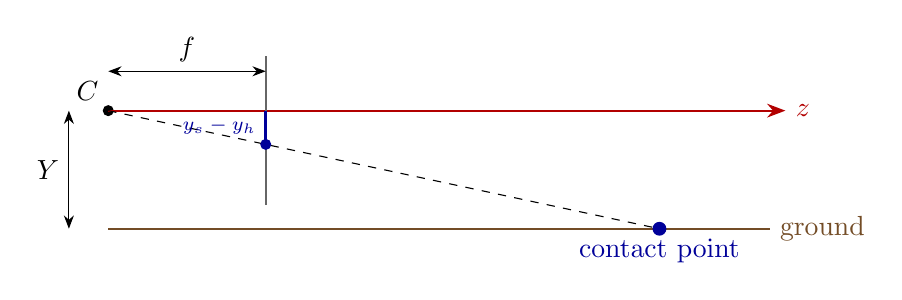
\begin{tikzpicture}[>=Stealth]
\fill (0,0) circle(2pt) node[above left]{$C$};
\draw[->,red!70!black,thick] (0,0)--(8.6,0) node[right]{$z$};
\draw[thick,black!60] (2,-1.2)--(2,0.7);
\draw[thick,brown!60!black] (0,-1.5)--(8.4,-1.5) node[right]{ground};
\draw[dashed] (0,0)--(7,-1.5);
\fill[blue!60!black] (7,-1.5) circle(2.5pt) node[below]{contact point};
\fill[blue!60!black] (2,-0.4286) circle(2pt);
\draw[very thick,blue!60!black] (2,0)--(2,-0.4286);
\node[left,blue!60!black] at (2,-0.2) {\scriptsize $y_s-y_h$};
\draw[<->] (-0.5,0)--(-0.5,-1.5) node[midway,left]{$Y$};
\draw[<->] (0,0.5)--(2,0.5) node[midway,above]{$f$};
\end{tikzpicture}
\caption{Vertical position (redrawn from slide 26, side view; horizon = optical axis for a level camera).}
\end{figure}
 
\begin{corollary}[Sensitivity]
Differentiating, $\delta z=z^2\,\delta y/(fY)$.
\end{corollary}
 
\begin{example}
$f=700$\,px, $Y=1.65$\,m, contact point $40$\,px below the horizon: $z=700\cdot1.65/40\approx28.9$\,m. A one-pixel error moves this by $z^2/(fY)\approx0.73$\,m.
\end{example}
 
\begin{intuition}
No knowledge of the object is required, only its contact point with the ground; but \emph{the assumptions carry the estimate}: flat ground, known camera height, known horizon. Note the resemblance to Proposition~\ref{prop:errlaw}: the error also grows as $z^2$, with the camera height $Y$ playing the role of a baseline (a remark of these notes, not on the slide). Cues near the horizon are extremely sensitive.
\end{intuition}
 
% =====================================================================
\section{Supervised Single-View Depth \slides{27--35}}
% =====================================================================
\emph{Paying with a prior, part two.} Fitting the prior requires an architecture, a loss that respects the scale ambiguity, and measured depth data.
 
\subsection{The Supervised Setup \slides{28}}
 
\begin{definition}[Supervised depth learning]
A training set of image / depth-map pairs, and a network from $3\times H\times W$ to $1\times H\times W$ trained with a per-pixel loss:
\[
\mathrm{TR}=\{(\bm I_i,\bm D_i)\}_{i=1}^{N},\qquad \hat{\bm D}=f_\theta(\bm I).
\]
\end{definition}
 
\begin{figure}[htbp]
\centering
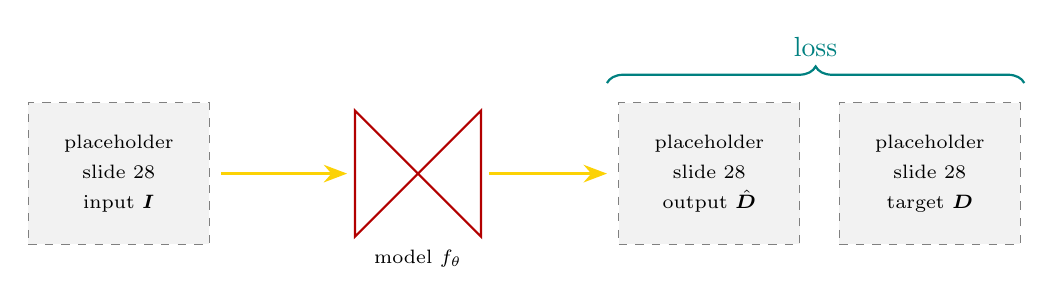
\begin{tikzpicture}[>=Stealth]
\node[draw=black!50,dashed,fill=black!5,minimum width=2.3cm,minimum height=1.8cm,align=center] (I) at (0,0) {\scriptsize placeholder\\[-1pt]\scriptsize slide 28\\[-1pt]\scriptsize input $\bm I$};
\draw[red!70!black,thick] (3,0.8)--(4.6,-0.8)--(4.6,0.8)--(3,-0.8)--cycle;
\node[below] at (3.8,-0.85) {\scriptsize model $f_\theta$};
\node[draw=black!50,dashed,fill=black!5,minimum width=2.3cm,minimum height=1.8cm,align=center] (P) at (7.5,0) {\scriptsize placeholder\\[-1pt]\scriptsize slide 28\\[-1pt]\scriptsize output $\hat{\bm D}$};
\node[draw=black!50,dashed,fill=black!5,minimum width=2.3cm,minimum height=1.8cm,align=center] (T) at (10.3,0) {\scriptsize placeholder\\[-1pt]\scriptsize slide 28\\[-1pt]\scriptsize target $\bm D$};
\draw[->,very thick,yellow!70!orange] (1.3,0)--(2.9,0);
\draw[->,very thick,yellow!70!orange] (4.7,0)--(6.2,0);
\draw[decorate,decoration={brace,amplitude=6pt},teal,thick] (6.2,1.15)--(11.5,1.15) node[midway,above=6pt,teal]{loss};
\end{tikzpicture}
\caption{The supervised setup (redrawn from slide 28; the two depth maps are photographs to copy from the slide).}
\end{figure}
 
\begin{intuition}
Data, network and per-pixel loss are the whole recipe; the slide's summary is that \emph{every remaining design decision is inside the loss} (\emph{what} counts as a correct prediction when scale is unobservable).
\end{intuition}
 
\subsection{Three Datasets \slides{29}}
 
Each of the three sits in a different cell of the principles table: a projected-pattern camera, a scanning laser, and triangulation with no known baseline.
 
\begin{itemize}
\item \textbf{NYU Depth v2}: indoor, from a structured-light depth camera, with its raw depth \emph{inpainted} to give a dense label.
\item \textbf{KITTI}: driving, LiDAR projected into the camera as in \S3.4.
\item \textbf{MegaDepth}: internet photo collections through structure from motion and multi-view stereo. Dense, varied, and \emph{scale-ambiguous by construction}.
\end{itemize}
 
These are the $\bm D_i$ of the previous slide. Each inherits the error sources of the sensor that produced it, and the last carries no metric scale at all -- which is what the next two methods are designed around.
 
\begin{table}[htbp]
\centering\footnotesize
\begin{tabular}{lllllr}
\toprule
Dataset & Annotation & Depth type & Accuracy & Diversity & \# images\\
\midrule
DIML Indoor & RGB-D & metric & medium & medium & 220K\\
MegaDepth & SfM & no scale & medium & medium & 130K\\
ReDWeb & stereo & no scale \& shift & medium & high & 3600\\
WSVD & stereo & no scale \& shift & medium & high & 1.5M\\
3D Movies & stereo & no scale \& shift & medium & high & 75K\\
DIW & user clicks & ordinal pair & low & high & 496K\\
ETH3D & laser & metric & high & low & 454\\
Sintel & synthetic & (metric) & high & medium & 1064\\
KITTI & laser/stereo & metric & medium & low & 93K\\
NYUDv2 & RGB-D & metric & medium & low & 407K\\
TUM-RGBD & RGB-D & metric & medium & low & 80K\\
\bottomrule
\end{tabular}
\caption{Trimmed transcription of the dataset table on slide 29 (the indoor/outdoor/dynamic/video/dense check-mark columns are omitted; copy the full table from the slide if needed).}
\end{table}
 
\begin{intuition}
Every dataset is a \emph{sensor's opinion} of depth. NYU inherits the holes and inpainting of a structured-light camera, KITTI inherits LiDAR sparsity and flying points, MegaDepth inherits SfM's arbitrary scale. Datasets with ``no scale \& shift'' or ``ordinal'' labels cannot be trained on with a plain L2 loss: the loss has to be told which ambiguity to ignore.
\end{intuition}
 
\subsection{The Scale-Invariant Loss \slides{30}}
 
The direct choice, $\mathcal D(\bm D,\hat{\bm D})=\|\bm D-\hat{\bm D}\|_2^2$, penalizes the network for a global scale the image does not determine. What is required is a loss invariant to that scale:
\[
\mathcal D(\bm y,\bm y^\ast)=\mathcal D(s\bm y,\bm y^\ast)\quad\forall s>0 .
\]
 
\begin{definition}[Eigen--Puhrsch--Fergus scale-invariant loss (NIPS 2014)]
Mean squared error in log space, plus a per-image offset:
\[
\mathcal D(\bm y,\bm y^\ast)=\frac1n\sum_{i=1}^n\big(\log y_i-\log y^\ast_i+\alpha\big)^2,
\qquad
\alpha=\frac1n\sum_{i=1}^n\big(\log y^\ast_i-\log y_i\big).
\]
\end{definition}
 
\begin{lemma}[Closed form and invariance]\label{lem:si}
Write $d_i=\log y_i-\log y^\ast_i$. Then $\alpha=-\bar d$ minimizes the expression over all offsets, and
\[
\mathcal D(\bm y,\bm y^\ast)=\frac1n\sum_i d_i^2-\frac1{n^2}\Big(\sum_i d_i\Big)^2=\operatorname{Var}(d_i).
\]
Moreover $\mathcal D(s\bm y,\bm y^\ast)=\mathcal D(\bm y,\bm y^\ast)$ for every $s>0$.
\end{lemma}
\begin{proof}
Differentiating $\sum_i(d_i+\alpha)^2$ in $\alpha$ and setting to zero gives $\alpha=-\bar d$; substituting yields $\frac1n\sum(d_i-\bar d)^2$, which is the stated variance. Replacing $\bm y$ by $s\bm y$ adds the constant $\log s$ to every $d_i$; a variance does not change under a constant shift. \qedhere
\end{proof}
 
\begin{figure}[htbp]
\centering
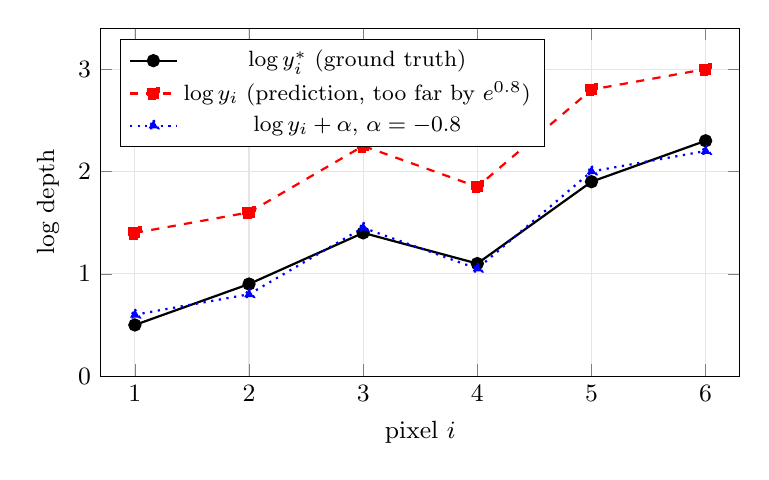
\begin{tikzpicture}
\begin{axis}[width=0.8\linewidth,height=6cm,xlabel={pixel $i$},ylabel={log depth},xmin=0.7,xmax=6.3,ymin=0,ymax=3.4,
  legend style={at={(0.03,0.97)},anchor=north west,font=\footnotesize},grid=both,grid style={gray!20}]
\addplot[black,thick,mark=*] coordinates {(1,0.5)(2,0.9)(3,1.4)(4,1.1)(5,1.9)(6,2.3)};
\addlegendentry{$\log y^\ast_i$ (ground truth)}
\addplot[red,thick,dashed,mark=square*] coordinates {(1,1.4)(2,1.6)(3,2.25)(4,1.85)(5,2.8)(6,3.0)};
\addlegendentry{$\log y_i$ (prediction, too far by $e^{0.8}$)}
\addplot[blue,thick,dotted,mark=triangle*] coordinates {(1,0.6)(2,0.8)(3,1.45)(4,1.05)(5,2.0)(6,2.2)};
\addlegendentry{$\log y_i+\alpha$, $\alpha=-0.8$}
\end{axis}
\end{tikzpicture}
\caption{Original toy example (not on the slides). The prediction has the right shape but a wrong global scale. Naive log-MSE would be $\approx0.646$; the scale-invariant loss, after aligning by $e^{\alpha}$, is only $\approx0.0058$.}
\end{figure}
 
\begin{intuition}
In log space a wrong \emph{scale} becomes a constant \emph{offset}, and the loss subtracts the best constant offset before looking at the errors. So only the \emph{shape} of the depth map is judged. Two side remarks from the slide: log space stops far pixels (numerically large) from dominating, and $e^{\alpha}\bm y$ is the scalar multiple that best aligns the prediction to the ground truth -- every scalar multiple of $\bm y$ scores identically.
\end{intuition}
 
\subsection{Output Spaces \slides{31}}
 
Five quantities a depth network can predict differ in how many unknowns are left free, and in \emph{what the free parameters act on}.
 
\begin{table}[htbp]
\centering\small
\begin{tabularx}{\linewidth}{@{}p{0.3cm}Ycp{3.1cm}Y@{}}
\toprule
& output & free param. & aligned by & trained this way to\\
\midrule
1 & metric depth & 0 & nothing & plan and measure\\
2 & scale-invariant depth & 1 ($s$) & one scale & share one scale per scene\\
3 & affine-invariant disparity & 2 ($s,t$) & scale and shift & mix datasets with no common zero\\
4 & affine-invariant depth & 2 ($s,t$) & scale and shift & mix datasets in depth (3.11)\\
5 & ordinal & any monotone map & nothing & rank only\\
\bottomrule
\end{tabularx}
\caption{Output spaces (slide 31). Scale-invariant: $\hat y\approx s\,y^\ast$; affine-invariant: $\hat q\approx s\,q^\ast+t$ with $q=1/y$ for disparity.}
\end{table}
 
These are routinely conflated: Eigen's log-space is \emph{one} parameter, affine invariance \emph{two}. The affine row appears twice because the same pair $(s,t)$ can act on disparity or on depth, and the two differ in 3D (next subsection). Benchmarks align the free parameters against the ground truth first, then score with $\delta$ and AbsRel, so a model is scored on \emph{shape, not on meters}.
 
\begin{example}[Standard metrics, background]
$\mathrm{AbsRel}=\frac1n\sum_i|\hat y_i-y^\ast_i|/y^\ast_i$, and $\delta_1$ is the fraction of pixels with $\max(\hat y_i/y^\ast_i,\,y^\ast_i/\hat y_i)<1.25$; both are computed after the alignment above.
\end{example}
 
\subsection{Affine Invariance in Disparity and in Depth \slides{32}}
 
\begin{proposition}[Affine map in disparity = projective map in space]\label{prop:affdisp}
An affine map in inverse depth,
\[
\frac1z\;\longmapsto\;\frac{s}{z}+t\quad\Longleftrightarrow\quad z\;\longmapsto\;\frac{z}{s+t\,z},
\]
is a nonlinear map in depth. Back-projecting the transformed depth gives $\hat{\bm p}=\bm p/(s+t\,p_z)$, which is a \emph{projective} map of space: planes remain planes.
\end{proposition}
\begin{proof}
$s/z+t=(s+tz)/z$, so $z\mapsto z/(s+tz)$. Back-projection by \eqref{eq:backproj}: $\hat{\bm p}=\frac{z}{s+tz}\Kinv\xt_s=\bm p/(s+tp_z)$. To see planes stay planes, let $\bm a^\top\bm p=c$ and $w=s+tp_z$. From $\hat{\bm p}=\bm p/w$ we get $\hat p_z=p_z/w$, hence $p_z=s\hat p_z/(1-t\hat p_z)$ and $w=s/(1-t\hat p_z)$, so $\bm p=w\hat{\bm p}$. Substituting, $s\,\bm a^\top\hat{\bm p}=c\,(1-t\hat p_z)$, which is linear in $\hat{\bm p}$. \qedhere
\end{proof}
 
\begin{figure}[htbp]
\centering
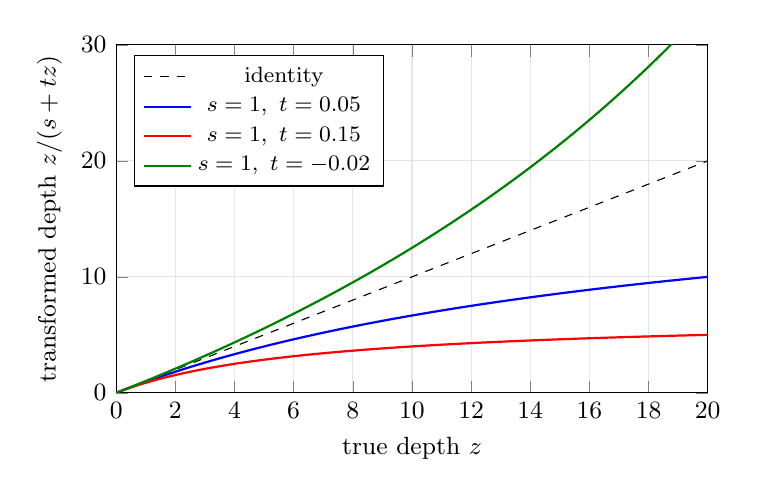
\begin{tikzpicture}
\begin{axis}[width=0.75\linewidth,height=6cm,xlabel={true depth $z$},ylabel={transformed depth $z/(s+tz)$},xmin=0,xmax=20,ymin=0,ymax=30,
  legend style={at={(0.03,0.97)},anchor=north west,font=\footnotesize},grid=both,grid style={gray!20}]
\addplot[black,dashed,domain=0:20,samples=2]{x};
\addlegendentry{identity}
\addplot[blue,thick,domain=0:20,samples=60]{x/(1+0.05*x)};
\addlegendentry{$s=1,\ t=0.05$}
\addplot[red,thick,domain=0:20,samples=60]{x/(1+0.15*x)};
\addlegendentry{$s=1,\ t=0.15$}
\addplot[green!50!black,thick,domain=0:20,samples=60]{x/(1-0.02*x)};
\addlegendentry{$s=1,\ t=-0.02$}
\end{axis}
\end{tikzpicture}
\caption{Original figure (not on the slides): an affine map in disparity acts on \emph{depth} as $z\mapsto z/(s+tz)$, a compressive or expansive warp, not a rescaling.}
\end{figure}
 
\begin{intuition}
A ground plane is therefore \emph{tilted, not bent}: you can decide a scale and shift wrongly, and flat things stay flat but the world may look sheared toward or away from the camera. An affine map in depth itself would instead be $z\mapsto sz+t$, a rigid stretch and translation along the ray. The two choices give the same 2-parameter count but \emph{different 3D geometry} -- the reason the table lists the affine row twice.
\end{intuition}
 
\subsection{MiDaS: Mixing the Datasets \slides{33}}
 
No single dataset covers the visual world, so MiDaS trains on several. The obstacle is that they disagree about what they measure (metric, no scale, no scale and shift, ordinal, ...). Its recipe:
\begin{itemize}
\item predict in \textbf{disparity space} (inverse depth up to scale and shift);
\item train with a \textbf{scale-and-shift-invariant loss}, where the alignment $(s,t)$ is a least-squares fit solved \emph{in closed form per image};
\item add a \textbf{multi-scale gradient matching} term, which is the gradient loss again, at four resolutions.
\end{itemize}
The output space is the affine-invariant \emph{disparity} row of the table, not the affine-invariant \emph{depth} row under it.
 
\begin{lemma}[Closed-form alignment]\label{lem:ssi}
For predictions $\hat q_i$ and targets $q^\ast_i$, the pair
\[
(s,t)=\arg\min_{s,t}\sum_i\big(s\,\hat q_i+t-q^\ast_i\big)^2
\]
is $s=\dfrac{\operatorname{Cov}(\hat q,q^\ast)}{\operatorname{Var}(\hat q)}$, $\;t=\bar q^\ast-s\,\bar{\hat q}$ (assuming $\operatorname{Var}(\hat q)>0$).
\end{lemma}
\begin{proof}
Setting $\partial/\partial t=0$ gives $t=\bar q^\ast-s\bar{\hat q}$. Setting $\partial/\partial s=0$: $s\sum\hat q_i^2+t\sum\hat q_i=\sum\hat q_iq_i^\ast$. Substituting $t$ and dividing by $n$: $s(\overline{\hat q^2}-\bar{\hat q}^2)=\overline{\hat qq^\ast}-\bar{\hat q}\bar q^\ast$. \qedhere
\end{proof}
 
The loss is then evaluated on the residual \emph{after} alignment. The gradient matching term, in its standard form, penalizes gradients of the aligned residual $R^k$ at each of the $K=4$ scales $k$: $\frac1M\sum_{k=1}^{K}\sum_i(|\nabla_xR^k_i|+|\nabla_yR^k_i|)$ (form from the original MiDaS paper; the slide only says ``the gradient loss again, at four resolutions'').
 
\begin{figure}[htbp]
\centering
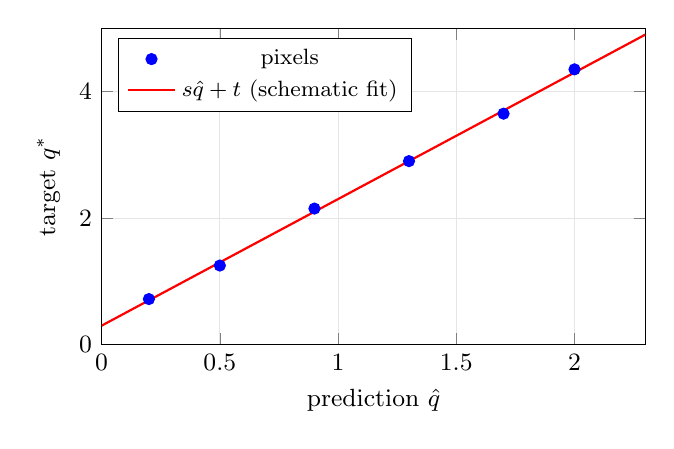
\begin{tikzpicture}
\begin{axis}[width=0.7\linewidth,height=5.6cm,xlabel={prediction $\hat q$},ylabel={target $q^\ast$},xmin=0,xmax=2.3,ymin=0,ymax=5,grid=both,grid style={gray!20},
  legend style={at={(0.03,0.97)},anchor=north west,font=\footnotesize}]
\addplot[only marks,mark=*,blue] coordinates {(0.2,0.72)(0.5,1.25)(0.9,2.15)(1.3,2.9)(1.7,3.65)(2.0,4.35)};
\addlegendentry{pixels}
\addplot[red,thick,domain=0:2.3,samples=2]{2*x+0.3};
\addlegendentry{$s\hat q+t$ (schematic fit)}
\end{axis}
\end{tikzpicture}
\caption{Original schematic (not on the slides): per-image least-squares alignment of a prediction to targets that use a different scale and zero.}
\end{figure}
 
\begin{intuition}
Each training image gets its \emph{own} best-fit $(s,t)$ before the network is judged, like a teacher who marks a student's drawing after allowing it to be enlarged and moved on the page. That is what lets one network learn from a metric laser dataset, an up-to-scale SfM dataset and a stereo-movie dataset at the same time. Working in \emph{disparity} matters because an unknown rig only contributes an unknown scale there (Corollary~\ref{cor:unknownb}).
\end{intuition}
 
\subsection{Depth Anything V2 \slides{34}}
 
Labeled depth data is the bottleneck, so the second version removes the requirement for it (the first version also trained on labeled real data).
 
\begin{algorithm}[Teacher--student training]
\begin{enumerate}[nosep]
\item Train a \textbf{teacher} on precise \emph{synthetic} images only, where depth is exact and complete.
\item Use the teacher to \textbf{pseudo-label} a very large set of unlabeled real photographs.
\item Train the \textbf{student} on those pseudo-labels.
\end{enumerate}
\end{algorithm}
 
Architecture and losses: encoder from self-supervised pretraining, decoder from dense prediction, and the \emph{same} scale-and-shift-invariant plus gradient-matching losses as MiDaS. The output space is affine-invariant inverse depth; metric models are a separate fine-tuning step on top.
 
\begin{figure}[htbp]
\centering
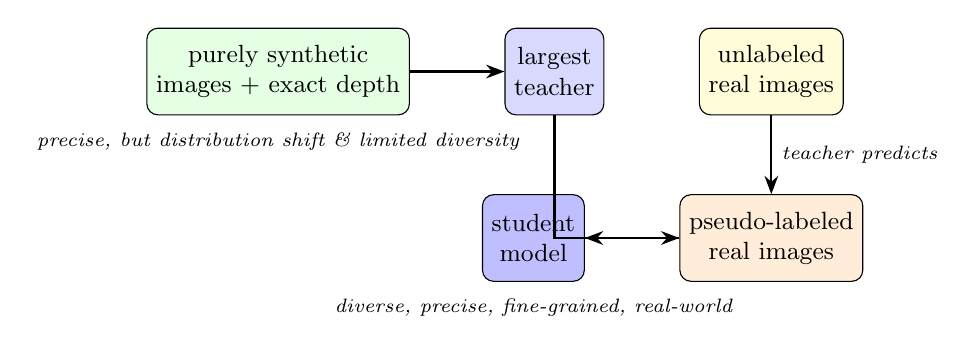
\begin{tikzpicture}[>=Stealth,node distance=6mm,
  box/.style={draw,rounded corners,minimum height=1.1cm,align=center,font=\small},
  tag/.style={font=\scriptsize\itshape}]
\node[box,fill=green!10] (syn) {purely synthetic\\images + exact depth};
\node[box,fill=blue!15,right=12mm of syn] (teach) {largest\\teacher};
\node[box,fill=yellow!15,right=12mm of teach] (unl) {unlabeled\\real images};
\node[box,fill=orange!15,below=10mm of unl] (pl) {pseudo-labeled\\real images};
\node[box,fill=blue!25,left=12mm of pl] (stud) {student\\model};
\draw[->,thick] (syn)--(teach);
\draw[->,thick] (unl)--(pl) node[midway,right,tag]{teacher predicts};
\draw[->,thick] (teach.south) |- (pl.west) ;
\draw[->,thick] (pl)--(stud);
\node[tag,below=1mm of syn]{precise, but distribution shift \& limited diversity};
\node[tag,below=1mm of stud]{diverse, precise, fine-grained, real-world};
\end{tikzpicture}
\caption{Depth Anything V2 pipeline (redrawn from slide 34).}
\end{figure}
 
\begin{intuition}
Synthetic images give \emph{perfect} labels but look unlike the real world; real photos look right but have no labels. The teacher transfers its precision to real photos through pseudo-labels, so the student sees real-world diversity with clean, fine-grained targets. The price: the student inherits what the teacher believes -- its prior -- rather than anything measured.
\end{intuition}
 
\subsection{Failure on Anamorphic Art \slides{35}}
 
Anamorphic street art is a flat pavement painted to look like a hole. The predicted depth map is wrong throughout, with no indication of uncertainty. Nothing has malfunctioned: the prior behaves as trained, on an input constructed to exploit it. \emph{The prior is both the method and the failure mode.}

 \begin{figure}[H]
	\centering
	\includegraphics[width=1.0\linewidth]{1790768347386.png}
	\caption{left: photo of a street painting of a clock tower on pavement; right: predicted depth map from MegaDepth demo}\label{fig:1790768347386}
 \end{figure}

\begin{figure}[htbp]
\centering
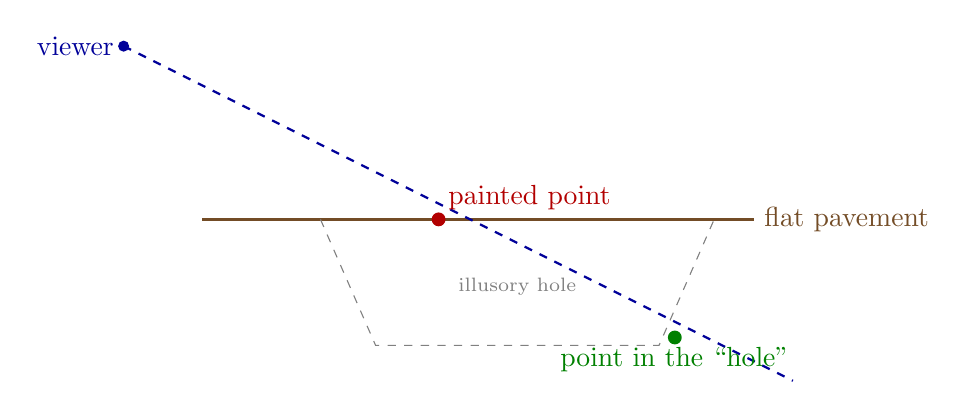
\begin{tikzpicture}[>=Stealth]
\fill[blue!60!black] (0,2.2) circle(2pt) node[left]{viewer};
\draw[very thick,brown!60!black] (1,0)--(8,0) node[right]{flat pavement};
\draw[dashed,thick,blue!60!black] (0,2.2)--(8.5,-2.05);
\fill[red!70!black] (4,0) circle(2.5pt) node[above right]{painted point};
\fill[green!50!black] (7,-1.5) circle(2.5pt) node[below]{point in the ``hole''};
\draw[dashed,gray] (2.5,0)--(3.2,-1.6)--(6.8,-1.6)--(7.5,0);
\node[gray] at (5,-0.85) {\scriptsize illusory hole};
\end{tikzpicture}
\caption{Original figure (not on the slides): from the painting's viewpoint the painted point on the flat ground and the point at the bottom of the imagined hole lie on the same ray (Proposition~\ref{prop:ray}). One image cannot distinguish them, so the network chooses the ``likely'' one.}
\end{figure}
 
\begin{intuition}
The picture is a concrete instance of the back-projected ray: the artist chooses a flat surface whose appearance is \emph{exactly} what a deep hole would look like from one viewpoint. Depth-from-one-image cannot know; it picks the answer its training data make most probable. Note also the ``no indication of uncertainty'': the network is confidently wrong.
\end{intuition}
 
% =====================================================================
\section{Cues Used by the Network \slides{36--39}}
% =====================================================================
\emph{What the prior turns out to be.} A monocular depth network is a prior fitted to a dataset. Three probes examine which image evidence that prior relies on.
 
\subsection{The Pasted-Car Experiment \slides{37}}
 
A car is cropped from the image and pasted back at a chosen ground contact point and a chosen scale, placing the two cues of \S3.6 in conflict: both correct (position \& size), \emph{position only}, or \emph{size only}. The finding (paraphrased): across four networks, the vertical position in the image wins over the apparent size of known obstacles.
\begin{itemize}
\item Position only tracks the true distance; size only does not.
\item The result holds across four networks.
\item Vertical position needs no object model and generalizes to objects absent from the training set.
\end{itemize}
 
 
\begin{figure}[H]
	\centering
	\includegraphics[width=1.0\linewidth]{1790768421548.png}
	\caption{grid of pasted-car examples (position \& size / position only / size only) with predicted depth maps}\label{fig:1790768421548}
\end{figure}

\begin{figure}[htbp]
\centering
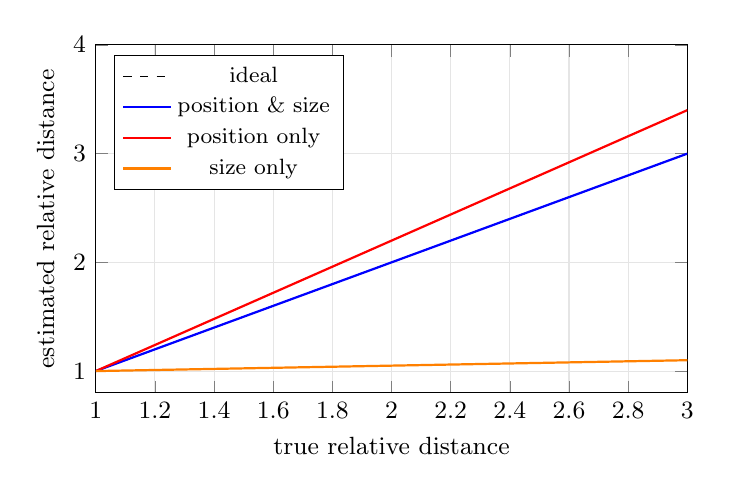
\begin{tikzpicture}
\begin{axis}[width=0.75\linewidth,height=6cm,xlabel={true relative distance},ylabel={estimated relative distance},xmin=1,xmax=3,ymin=0.8,ymax=4,
  legend style={at={(0.03,0.97)},anchor=north west,font=\footnotesize},grid=both,grid style={gray!20}]
\addplot[black,dashed,domain=1:3,samples=2]{x};
\addlegendentry{ideal}
\addplot[blue,thick,domain=1:3,samples=2]{1+1.0*(x-1)};
\addlegendentry{position \& size}
\addplot[red,thick,domain=1:3,samples=2]{1+1.2*(x-1)};
\addlegendentry{position only}
\addplot[orange,thick,domain=1:3,samples=2]{1+0.05*(x-1)};
\addlegendentry{size only}
\end{axis}
\end{tikzpicture}
\caption{\textbf{Qualitative schematic} after the plot on slide 37, not measured data: positional cues track the ideal line (with some overestimate and larger spread), size-only stays almost flat.}
\end{figure}
 
\begin{intuition}
The networks behave like the vertical-position cue of Proposition~\ref{prop:vertical}, not like Proposition~\ref{prop:size}. Sensible: vertical position works for \emph{anything} touching the ground, whereas size needs a size prior per object class. But it also means a car pasted ``floating'' higher in the frame is judged farther, even if it appears huge.
\end{intuition}
 
\subsection{Pitch and Roll \slides{38}}
 
A pitch change is simulated with a vertical crop and a roll with a rotated crop; both are recovered from the predicted depth. Findings: the networks \textbf{only partially} track camera orientation, and small pitch changes measurably disturb the estimated distance to obstacles.
 
\begin{figure}[htbp]
\centering
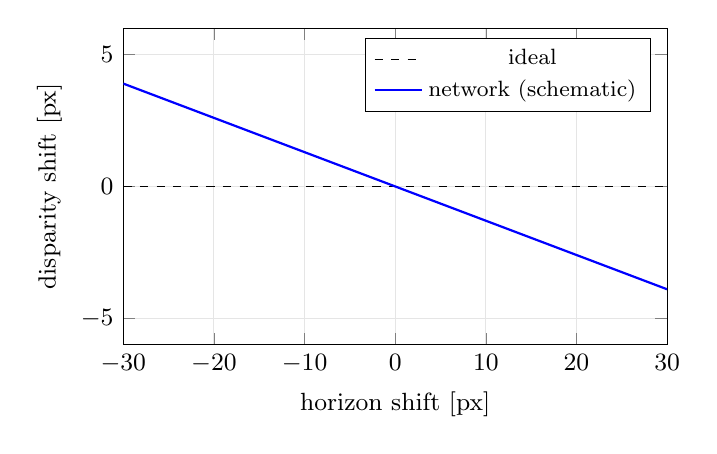
\begin{tikzpicture}
\begin{axis}[width=0.7\linewidth,height=5.6cm,xlabel={horizon shift [px]},ylabel={disparity shift [px]},xmin=-30,xmax=30,ymin=-6,ymax=6,grid=both,grid style={gray!20},
  legend style={at={(0.97,0.97)},anchor=north east,font=\footnotesize}]
\addplot[black,dashed,domain=-30:30,samples=2]{0};
\addlegendentry{ideal}
\addplot[blue,thick,domain=-30:30,samples=2]{-0.13*x};
\addlegendentry{network (schematic)}
\end{axis}
\end{tikzpicture}
\caption{\textbf{Qualitative schematic} after the plot on slide 38, not measured data: an ideal system would ignore the crop (zero shift), the networks' output drifts roughly linearly and opposite to the horizon shift.}
\end{figure}
 
\begin{intuition}
A crop does \emph{not} change an object's distance to the horizon, $y_s-y_h$, so by Proposition~\ref{prop:vertical} the true depth cannot change. But it does change the object's \emph{absolute} vertical position, and the predictions change with it. The network reads vertical image position, rather than distance to the horizon -- exactly the shortcut warned about in \S3.6, where the horizon depends on pitch and roll only.
\end{intuition}
 
\subsection{Dependence on the Training Camera \slides{39}}
 
A third probe: what happens when only the \emph{camera} changes. A network trained at one focal length predicts the wrong depth at another, with the scene held identical. The apparent-size relation (Proposition~\ref{prop:size}) contains $f$, and the network has absorbed the training value as a constant. Supplying the intrinsics to the network as extra input channels removes most of the error. The slide's summary: the prior is fitted to the training \emph{camera} as much as to the training \emph{scenes}.
 
\begin{proposition}[Idealized focal-length bias -- worked consequence, not on the slide]\label{prop:focal}
Suppose a network has absorbed $z=f_0H/h$ with the training focal length $f_0$. At test focal length $f$ the image height is $h'=fH/z$, so the predicted depth is
\[
\hat z=\frac{f_0H}{h'}=\frac{f_0}{f}\,z .
\]
\end{proposition}
 
\begin{figure}[htbp]
\centering
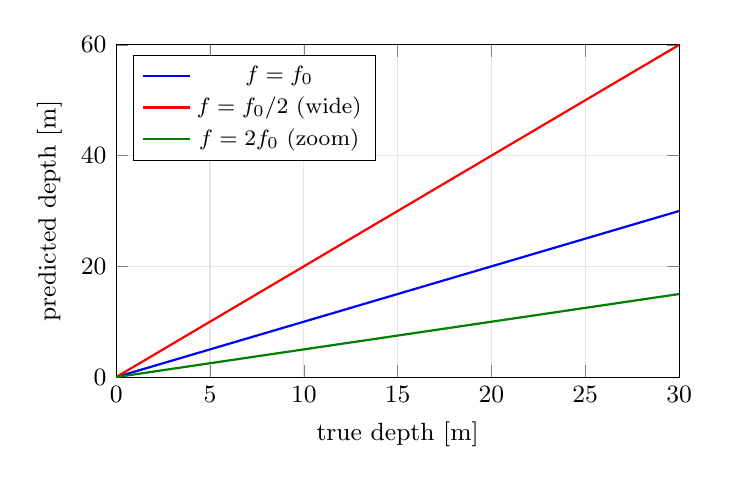
\begin{tikzpicture}
\begin{axis}[width=0.72\linewidth,height=5.8cm,xlabel={true depth [m]},ylabel={predicted depth [m]},xmin=0,xmax=30,ymin=0,ymax=60,grid=both,grid style={gray!20},
  legend style={at={(0.03,0.97)},anchor=north west,font=\footnotesize}]
\addplot[blue,thick,domain=0:30,samples=2]{x};
\addlegendentry{$f=f_0$}
\addplot[red,thick,domain=0:30,samples=2]{2*x};
\addlegendentry{$f=f_0/2$ (wide)}
\addplot[green!50!black,thick,domain=0:30,samples=2]{0.5*x};
\addlegendentry{$f=2f_0$ (zoom)}
\end{axis}
\end{tikzpicture}
\caption{Original figure (not on the slides): predicted depth under the idealization of Proposition~\ref{prop:focal}.}
\end{figure}
 
\begin{intuition}
Zooming in makes everything look bigger, and a network that silently assumes the training focal length reads ``bigger'' as ``closer''. This is a scale error, so it is precisely the kind of ambiguity metric prediction must resolve -- giving the network the intrinsics removes the hidden constant.
\end{intuition}

% =====================================================================
\section*{Next: Self-Supervision and a Generative Prior \slides{40}}
\addcontentsline{toc}{section}{Next: Self-Supervision and a Generative Prior \emph{(slide 40)}}

Part~I closes owing two debts: the prior was fitted to labels that a sensor had to measure, and mixing those labels cost two free parameters. Part~II removes the labels, then pays back the two numbers.

\section*{Part I in One Slide \slides{1--2}}
\addcontentsline{toc}{section}{Overview: Part I in One Slide \emph{(slides 1--2)}}
%=====================================================================
Part~I obtained depth in two ways and closed \emph{owing two debts}:
\begin{itemize}[nosep]
  \item \textbf{Time.} A laser measures range directly: metric and exact where it lands, but sparse, and it produces the labels everything else trains on.
  \item \textbf{A prior.} A network fitted to those labels is dense and cheap, but it \emph{predicts} rather than recovers depth. The prior was fitted to labels that a sensor had to measure.
\end{itemize}
Mixing labels of different origin moved the output down a table, at a cost of free parameters.

\begin{definition}[Output types and their free parameters]
A depth-like output is defined only up to a transformation, and each transformation leaves free parameters that something else must later fix.
\begin{center}\small
\begin{tabular}{@{}lcl@{}}\toprule
output & free parameters & aligned by\\\midrule
metric depth & 0 & nothing\\
scale-invariant depth & 1 & one scale $s$\\
affine-invariant disparity or depth & 2 & scale and shift $(s,t)$\\
ordinal & any monotone map & nothing\\\bottomrule
\end{tabular}
\end{center}
\end{definition}

\begin{intuition}
Each free parameter is a \emph{number a sensor must still supply}. If a network says ``this pixel is twice as far as that one'', it has told you shape but not meters. Example: the truth is $D=2.0\,\hat D+0.3$~m. A metric network outputs $D$ itself; an affine-invariant one outputs $\hat D$ and you need the pair $(2.0,\,0.3)$ to recover meters. The whole lecture is about who supplies those numbers: the baseline of a stereo rig, a large generative prior, or a handful of LiDAR returns.
\end{intuition}

%=====================================================================
\section{Supervision without Ground Truth \slides{3--6}}
%=====================================================================
This is section 3.9 of the lecture. Its thesis: \emph{a stereo pair supplies its own supervision, provided the warp connecting the two images is differentiable.}

\subsection{View Synthesis and the Backward Warp \slides{4}}
Training uses stereo pairs $\{(\bm I_L,\bm I_R)\}$ only; there is no depth anywhere in the training set. The objective is to reproduce one image of the pair from the other. Depth is the only internal quantity that makes this task solvable, so if the network solves it, depth is what it must have learned. This holds only where a pixel is \textbf{textured} and visible in \textbf{both} views; elsewhere the objective says nothing and a hand-written prior fills the gap.

\begin{definition}[Backward warp]
Given a disparity map $d(u,v)$ defined on the \emph{target} image, the backward warp synthesizes the target from the source by
\begin{equation}
\tilde{\bm I}_L(u,v)=\bm I_R\bigl(u-d(u,v),\,v\bigr).
\end{equation}
Every \emph{target} pixel is mapped to exactly one \emph{source} location.
\end{definition}

\begin{proposition}[Why the warp must be backward]
Forward mapping (pushing each source pixel to a target location) lets several sources land on one target pixel and leaves other target pixels empty: collisions and holes. Backward mapping assigns each target pixel exactly one value, which makes the warp a \emph{differentiable function} of $d$ rather than a scatter operation.
\end{proposition}

\begin{figure}[H]
\centering
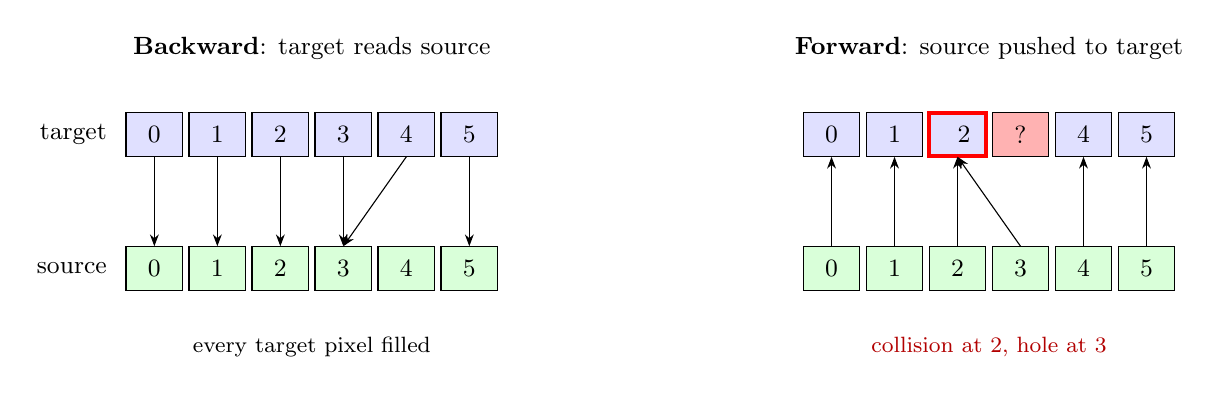
\begin{tikzpicture}[x=0.8cm,y=1cm,font=\small,
  pix/.style={draw,minimum width=0.72cm,minimum height=0.55cm,inner sep=0,fill=blue!12}]
\begin{scope}
 \node at (2.5,3.3) {\textbf{Backward}: target reads source};
 \foreach \i in {0,...,5}{\node[pix] (bt\i) at (\i,2.2){\i}; \node[pix,fill=green!15] (bs\i) at (\i,0.5){\i};}
 \node[anchor=east] at (-0.6,2.2){target}; \node[anchor=east] at (-0.6,0.5){source};
 \foreach \t/\s in {0/0,1/1,2/2,3/3,4/3,5/5}{\draw[-{Stealth[length=1.5mm]}] (bt\t.south)--(bs\s.north);}
 \node[font=\footnotesize,align=center] at (2.5,-0.5){every target pixel filled};
\end{scope}
\begin{scope}[xshift=8.6cm]
 \node at (2.5,3.3) {\textbf{Forward}: source pushed to target};
 \foreach \i in {0,...,5}{\node[pix] (ft\i) at (\i,2.2){\i}; \node[pix,fill=green!15] (fs\i) at (\i,0.5){\i};}
 \node[pix,fill=red!30] at (3,2.2){?};
 \node[pix,ultra thick,draw=red] at (2,2.2){\phantom{0}2};
 \foreach \s/\t in {0/0,1/1,2/2,3/2,4/4,5/5}{\draw[-{Stealth[length=1.5mm]}] (fs\s.north)--(ft\t.south);}
 \node[font=\footnotesize,align=center,text=red!70!black] at (2.5,-0.5){collision at 2, hole at 3};
\end{scope}
\end{tikzpicture}
\caption{Original 1D illustration of backward versus forward mapping (slide 4 shows the same effect on small coloured grids).}
\end{figure}

\begin{intuition}
Think of filling in a form versus mailing letters. Backward warping is the form: each target pixel asks \emph{``where in the other image should I look?''} and gets exactly one answer. Forward warping is the post office: every source pixel is mailed to an address; some mailboxes get two letters (collision), others none (hole), and ``two letters or none'' has no useful gradient. Note the sign convention: slide~4 writes $u-d$ for the left image as target, slide~5 writes $+d$ for a target/source pair set up the other way round; only the consistent use matters.
\end{intuition}

\subsection{Image Reconstruction as Supervision \slides{5}}
The pipeline of slide~5 has three steps: (1) a deep CNN predicts an inverse depth from the left image; (2) the right image is warped with it into a synthetic left image; (3) the reconstruction error against the real left image is the loss.

\begin{definition}[Disparity and photometric loss]
Under a rectified stereo rig with focal length $f$ and baseline $b$, the predicted inverse depth is the disparity
\begin{equation}
d(\bm p)=\frac{f\,b}{z(\bm p)}.
\end{equation}
The self-supervised loss compares the warped and real image,
\begin{equation}
\mathcal L_{\text{photo}}=\sum_{\bm p}\bigl\|\tilde{\bm I}(\bm p)-\bm I_L(\bm p)\bigr\|,\qquad \tilde{\bm I}(\bm p)=\bm I_R\bigl(\bm p+d(\bm p)\bigr).
\end{equation}
\end{definition}

\begin{figure}[H]
\centering
\begin{tikzpicture}[font=\small]
\node[box] (IL) at (0,0) {left image\\$\bm I_L$};
\node[box] (cnn) at (3.2,0) {deep CNN};
\node[box] (d) at (6.6,0) {inverse depth\\$d=fb/z$};
\node[box] (warp) at (6.6,-2.2) {warp\\$\tilde{\bm I}(\bm p)=\bm I_R(\bm p+d)$};
\node[box] (IR) at (2.6,-2.2) {right image\\$\bm I_R$};
\node[box,fill=orange!20] (loss) at (3.6,-4.2) {photometric loss $\|\tilde{\bm I}-\bm I_L\|$};
\draw[arr] (IL)--(cnn); \draw[arr] (cnn)--(d); \draw[arr] (d)--(warp);
\draw[arr] (IR)--(warp);
\draw[arr] (warp.south) |- (loss.east);
\draw[arr] (IL.south) |- (loss.west);
\end{tikzpicture}
\caption{Self-supervised stereo training (redrawn from slide 5). No depth label appears anywhere.}
\end{figure}

\begin{figure}[H]
	\centering
	\includegraphics[width=1.0\linewidth]{1790765520552.png}
	\caption{the KITTI street scene: left image, predicted inverse-depth map, warped image and reconstruction-error map (steps 1--3, with the red marker point)}\label{fig:1790765520552}
\end{figure}
\begin{intuition}
Depth is the \emph{only} unknown the network can vary to make the warped image match the real one, so a network that solves the task has learned depth. Worked numbers (illustrative): with $f=700$~px and $b=0.5$~m, a car at $z=10$~m has $d=35$~px, whereas at $z=70$~m it has only $d=5$~px. Disparity is \emph{inverse} depth: distant objects move the image little, so the training signal is weak at range.
\end{intuition}

\subsection{Where the Loss Is Blind \slides{6}}
\begin{proposition}[Blind spots of the photometric loss]
(a) \emph{Textureless regions.} Writing the residual as $r=\bm I_R(u-d)-\bm I_L(u)$ and the squared loss as $\tfrac12 r^2$,
\begin{equation}
\frac{\partial \mathcal L}{\partial d}=-\,r\cdot \bm I_R'(u-d),
\end{equation}
which vanishes wherever $\bm I(u_0+1)\approx \bm I(u_0)$ (flat image, zero derivative): such pixels receive \emph{no training signal at all}.\\
(b) \emph{Occlusions.} A pixel visible to one camera only has no match in the other view, so the residual there is meaningless.
\end{proposition}

Both gaps are filled by hand-written priors: a smoothness term, left-right consistency, a minimum over the two reprojections, and masking of pixels that do not move between frames.

\begin{proposition}[The baseline decides what the trained model is worth]
Trained on a stereo pair, the model inherits the known baseline $b$ and is metric \emph{for that rig}. Trained on video, the baseline is unknown, so the output is shape up to one global scale and every image needs its own alignment.
\end{proposition}

\begin{intuition}
The photometric loss is a detective that only works with clues. Flat white wall: no clue, no gradient, so the smoothness prior guesses. Something hidden from one eye: no partner to compare with. The baseline is the ruler: with stereo the ruler length $b$ is known, so meters come free; with a monocular video the ruler length is not known, so you get a beautiful shape in unknown units (one free parameter, as in the table of Section~1).
\end{intuition}

%=====================================================================
\section{Diffusion, From Scratch \slides{7--22}}
%=====================================================================
This is section 3.10. Its thesis: \emph{a model trained to remove noise is a prior: it points toward the data from anywhere in the space, and it can be sampled, conditioned or steered.} (Adapted on the slides from MIT 6.S183, Lecture~1, by D.~Pfrommer.)

\subsection{Supervised Learning \slides{8}}
Supervised learning fits \textbf{one output per input}. At a depth edge that output is the average of the near surface and the far one: a distance that belongs to neither.

\begin{proposition}[MSE regression returns the conditional mean]
Let $Y$ be the target and $\bx$ the input. Among all functions $f$, the minimizer of $\E\|f(\bx)-Y\|^2$ is $f^\star(\bx)=\E[Y\mid\bx]$.
\end{proposition}
\begin{proof}
For fixed $\bx$ with $m=\E[Y\mid \bx]$, $\E[\|f-Y\|^2\mid\bx]=\|f-m\|^2+\E[\|Y-m\|^2\mid\bx]$; the second term does not depend on $f$, and the first is minimized by $f=m$.
\end{proof}

\begin{intuition}
At a depth edge half the training examples say $2$~m (near surface) and half say $10$~m (far surface). The best single answer under squared error is $6$~m, which is the depth of \emph{nothing}. That is the blurred, flying-pixel edge of regression networks.
\end{intuition}

\subsection{Generative Learning \slides{9}}
A generative model fits a \textbf{distribution} over outputs, not one value. ``The band is what a diffusion model represents.''

\begin{figure}[H]
\centering
\begin{tikzpicture}
\begin{axis}[width=0.75\linewidth,height=5cm,domain=0:12,samples=200,axis lines=left,
  xlabel={depth at an edge pixel (m)},ylabel={density},ymajorticks=false,
  legend style={at={(0.98,0.98)},anchor=north east,font=\footnotesize}]
\addplot[thick,blue]{0.5*exp(-(x-2)^2/0.18)+0.5*exp(-(x-10)^2/0.72)};
\addplot[thick,red,dashed,samples=2] coordinates {(6,0)(6,0.6)};
\legend{true conditional distribution,regression output (mean)}
\end{axis}
\end{tikzpicture}
\caption{Original toy figure: a bimodal conditional distribution at a depth edge. The regressor answers the mean, which lies in a gap where the density is zero; a generative model can return a sample from one of the two modes.}
\end{figure}

\subsection{Many Outputs for One Input -- Text to Image \slides{10}}
One conditioning input has many valid completions. A regressor averages them; a diffusion model picks one.

\begin{figure}[H]
	\centering
	\includegraphics[width=1.0\linewidth]{1790765807667.png}
	\caption{left: grid of ``wearing\_glasses'' faces from regression (the mean face, blurred); right: grid of latent-diffusion samples (one sample, sharp)}\label{fig:1790765807667}
\end{figure}

\begin{intuition}
Blur is not a training failure. It is the correct answer to the wrong question: the conditional mean of a set of sharp images is not a sharp image. The same averaging is what flattens a depth edge.
\end{intuition}

\subsection{The Forward and Reverse Process \slides{11}}
The \textbf{forward process} adds noise to data one step at a time until nothing of the data is left. It is fixed and has no parameters. It is inspired by Brownian motion (many small independent displacements), and after enough steps the sample is indistinguishable from Gaussian noise. A diffusion model learns the \textbf{reverse process}, which recovers data from noise; that reverse process \emph{is the prior}.

\begin{definition}[Forward and reverse processes]
The forward chain $q(\bx_t\mid\bx_{t-1})$ maps $\bx_0$ (data) to $\bx_T$ (noise) and is fixed; the model $p_\theta(\bx_{t-1}\mid\bx_t)$ learns the way back.
\end{definition}

\begin{figure}[H]
\centering
\begin{tikzpicture}[font=\small]
\node[draw,circle,fill=gray!30,minimum size=1cm] (xT) at (0,0){$\bx_T$};
\node at (1.7,0){$\cdots$};
\node[draw,circle,fill=gray!30,minimum size=1cm] (xt) at (3.4,0){$\bx_t$};
\node[draw,circle,fill=gray!30,minimum size=1cm] (xt1) at (7,0){$\bx_{t-1}$};
\node at (8.7,0){$\cdots$};
\node[draw,circle,minimum size=1cm] (x0) at (10.4,0){$\bx_0$};
\draw[arr] (xT)--(1.2,0); \draw[arr] (2.2,0)--(xt);
\draw[arr] (xt)--node[above]{$p_\theta(\bx_{t-1}\mid\bx_t)$}(xt1);
\draw[arr] (xt1)--(8.2,0); \draw[arr] (9.2,0)--(x0);
\draw[arr,dashed] (xt1.south) to[bend left=25] node[below]{$q(\bx_t\mid\bx_{t-1})$} (xt.south);
\node[font=\footnotesize,gray] at (0,-1.1){noise}; \node[font=\footnotesize,gray] at (10.4,-1.1){data};
\end{tikzpicture}
\caption{Forward (dashed, fixed) and reverse (solid, learned) chains, redrawn from slide 11.}
\end{figure}

\begin{figure}[H]
\centering
\begin{tikzpicture}
\begin{axis}[width=0.6\linewidth,height=4.3cm,domain=0:100,samples=50,axis lines=left,xlabel={$t$},ylabel={$X_t$},
  legend style={font=\footnotesize,at={(0.03,0.97)},anchor=north west}]
\addplot[thick,blue]{sqrt(x)}; \addplot[thick,blue]{-sqrt(x)}; \addplot[dashed,gray]{0};
\legend{$\pm\sqrt{t}$ (std.\ dev.\ envelope)}
\end{axis}
\end{tikzpicture}
\caption{Original figure: the spread of a random walk grows like $\sqrt t$, the mechanism that buries the data in noise.}
\end{figure}
\begin{figure}[H]
	\centering
	\includegraphics[width=1.0\linewidth]{1790765932964.png}
	\caption{Brownian-motion simulated paths (coloured bundle of trajectories) with the histogram of $X_T$ on the right, and the two small face images (noisy, clean) below the chain}\label{fig:1790765932964}
\end{figure}
\subsection{Training by Noise Prediction \slides{12}}
A denoising diffusion model estimates the noise vector $\beps$ from a noise level $\sigma>0$ and a noisy input $\bx_\sigma\approx\bx_0+\sigma\beps$, where $\bx_0$ lies on the data manifold $\mathcal{K}\subset\R^n$.

\begin{definition}[Denoiser and training loss]
A denoiser $\beps_\theta:\R^n\times\R_+\to\R^n$ is learned by minimizing
\begin{equation}\label{eq:lsimple}
L_{\text{simple}}(\theta):=\E_{\bx_0,\sigma,\beps}\Bigl[\bigl\|\beps_\theta(\bx_0+\sigma\beps,\sigma)-\beps\bigr\|^2\Bigr],
\end{equation}
with $\bx_0$ sampled from the training data, $\sigma$ from a training noise schedule, and $\beps\sim\mathcal N(\bm 0,\bm I)$.
\end{definition}

\begin{intuition}
The recipe is three lines: take a clean example, add noise of a random strength you remember, and ask the network ``what noise did I add?''. Subtracting the guessed noise gives the guessed clean point, $\hat\bx_0=\bx_\sigma-\sigma\beps_\theta$. No labels beyond the data itself are needed.
\end{intuition}

\subsection{The Spiral Toy Model \slides{13}}
Everything that follows is shown on a 2D data set, where the prior is visible: \emph{it is where the points are}. The data are points of a 2D spiral $\bx_0$. The network is a fully connected MLP fed with $\bx_0+\sigma\beps$ and a 2D noise-level embedding of $\sigma$, and it predicts the noise.

\begin{lstlisting}
def get_sigma_embeds(sigma):
    sigma = sigma.unsqueeze(1)
    return torch.cat([torch.sin(torch.log(sigma)/2),
                      torch.cos(torch.log(sigma)/2)], dim=1)

class TimeInputMLP(nn.Module):
    def __init__(self, dim, hidden_dims):
        super().__init__()
        layers = []
        for in_dim, out_dim in pairwise((dim + 2,) + hidden_dims):
            layers.extend([nn.Linear(in_dim, out_dim), nn.GELU()])
        layers.append(nn.Linear(hidden_dims[-1], dim))
        self.net = nn.Sequential(*layers)
        self.input_dims = (dim,)

    def forward(self, x, sigma):
        sigma_embeds = get_sigma_embeds(sigma)
        nn_input = torch.cat([x, sigma_embeds], dim=1)
        return self.net(nn_input)

model = TimeInputMLP(dim=2, hidden_dims=(16,128,128,128,128,16))
\end{lstlisting}

\begin{intuition}
The extra two inputs $(\sin,\cos)$ of $\log\sigma/2$ tell the network \emph{how noisy} its input is. This matters because the right answer depends on $\sigma$: at small $\sigma$ the noise is a small nudge off the nearest data point, at large $\sigma$ the input is almost pure noise. Note that the first layer has width $\text{dim}+2=4$: two coordinates plus the two embedding numbers.
\end{intuition}

\subsection{Training the Toy Model \slides{14}}
\begin{lstlisting}
def training_loop(loader, model, schedule, epochs=10000):
    optimizer = torch.optim.Adam(model.parameters())
    for _ in range(epochs):
        for x0 in loader:
            optimizer.zero_grad()
            sigma, eps = generate_train_sample(x0, schedule)
            eps_hat = model(x0 + sigma * eps, sigma)
            loss = nn.MSELoss()(eps_hat, eps)
            loss.backward()
            optimizer.step()
\end{lstlisting}
The learned denoiser can be drawn as a \textbf{vector field} by plotting $\bx-\sigma\beps_\theta(\bx,\sigma)$. \emph{At small noise the arrows point at the nearest data. At large noise they point at the middle of the whole data set.} The slide's training curve falls from about $0.70$ to about $0.41$ over 15\,000 epochs.

\begin{figure}[H]
\centering
\begin{tikzpicture}[scale=2.1]
\begin{scope}
 \draw[blue,thick,domain=1:12,samples=100,smooth,variable=\t] plot ({0.08*\t*cos(\t r)},{0.08*\t*sin(\t r)});
 \foreach \t in {3,4.5,6,7.5,9,10.5}{
   \draw[-{Stealth[length=1.6mm]},red] ({1.3*0.08*\t*cos(\t r)},{1.3*0.08*\t*sin(\t r)})--({0.08*\t*cos(\t r)},{0.08*\t*sin(\t r)});
   \fill[red] ({1.3*0.08*\t*cos(\t r)},{1.3*0.08*\t*sin(\t r)}) circle (0.012);}
 \node at (0,-1.15) {small $\sigma$: toward the nearest data};
\end{scope}
\begin{scope}[xshift=3cm]
 \draw[blue,thick,domain=1:12,samples=100,smooth,variable=\t] plot ({0.08*\t*cos(\t r)},{0.08*\t*sin(\t r)});
 \foreach \a in {0,45,...,315}{\draw[-{Stealth[length=1.6mm]},red] (\a:1.15)--(\a:0.35);}
 \node at (0,-1.35) {large $\sigma$: toward the middle};
\end{scope}
\end{tikzpicture}
\caption{Original sketch of the denoiser field on the spiral (compare slide 14).}
\end{figure}

\begin{remark}[Why the loss does not reach zero]
The curve plateaus near $0.41$, not $0$. This is expected: even the best possible denoiser cannot recover $\beps$ exactly, because many $(\bx_0,\beps)$ pairs produce the same $\bx_\sigma$; the floor equals the average posterior variance of $\beps$ (Appendix~\ref{app:supp}, item~\ref{app:floor}).
\end{remark}

\subsection{The Ideal Denoiser \slides{15}}
The \textbf{ideal denoiser} minimizes the training loss; it is a function of the data set $\mathcal{K}$ and the noise level, and nothing else:
\begin{equation}
\beps^\ast:=\argmin_{\beps_\theta}\E_{\bx_0,\sigma,\beps}\bigl\|\beps_\theta(\bx_0+\sigma\beps,\sigma)-\beps\bigr\|^2 .
\end{equation}

\begin{theorem}[Ideal denoiser for a finite data set]\label{thm:ideal}
For a finite $\mathcal{K}$ (data uniformly distributed on $\mathcal{K}$, Gaussian noise),
\begin{equation}
\beps^\ast(\bx_\sigma,\sigma)=\frac{\sum_{\bx_0\in\mathcal{K}}(\bx_\sigma-\bx_0)\,\exp\!\bigl(-\|\bx_\sigma-\bx_0\|^2/2\sigma^2\bigr)}{\sigma\sum_{\bx_0\in\mathcal{K}}\exp\!\bigl(-\|\bx_\sigma-\bx_0\|^2/2\sigma^2\bigr)} .
\end{equation}
It is a weighted average of all data points: nearer points count more.
\end{theorem}
\begin{proof}
By the conditional-mean proposition, $\beps^\ast(\bx_\sigma,\sigma)=\E[\beps\mid\bx_\sigma]$ with $\beps=(\bx_\sigma-\bx_0)/\sigma$. By Bayes, $p(\bx_0\mid\bx_\sigma)\propto\exp(-\|\bx_\sigma-\bx_0\|^2/2\sigma^2)$ on $\mathcal{K}$. Taking the expectation of $(\bx_\sigma-\bx_0)/\sigma$ under these weights gives the formula.
\end{proof}

\begin{intuition}
Worked 1D example with $\mathcal{K}=\{-1,+1\}$, $\bx_\sigma=0.2$. For $\sigma=0.5$ the weights are $e^{-1.44/0.5}\approx0.056$ (for $-1$) and $e^{-0.64/0.5}\approx0.278$ (for $+1$), giving $\beps^\ast\approx-0.93$ and clean estimate $\hat\bx_0=0.2-0.5\cdot(-0.93)\approx0.66$: pulled toward the nearer point $+1$. For a large $\sigma=5$ the two weights are almost equal ($0.972$ vs $0.987$), $\beps^\ast\approx0.04$ and $\hat\bx_0\approx0.01$: the arrow points at the middle of the data set, exactly as in the slide's three panels ($\sigma=0.01,0.1,0.5$).
\end{intuition}

\subsection{The Smoothed Distance Function \slides{16}}
The distance to a set, $\mathrm{dist}_\mathcal{K}(\bx):=\inf\{\|\bx-\bx_0\|:\bx_0\in\mathcal{K}\}$, is not differentiable everywhere, so its gradient is hard to learn. Smoothing it by $\sigma$ fixes that.

\begin{definition}[Smoothed distance]
\begin{equation}
D_\sigma(\bx):=-\sigma^2\log\Bigl(\sum_{\bx_0\in\mathcal{K}}\exp\bigl(-\|\bx_0-\bx\|^2/2\sigma^2\bigr)\Bigr).
\end{equation}
(The slide denotes the smoothed squared distance by $\mathrm{dist}^2_\mathcal{K}(\bx,\sigma)$ and writes the identity below with a factor $\tfrac12$; with the definition as printed, $\tfrac12\mathrm{dist}^2_\mathcal{K}(\bx,\sigma)$ corresponds to $D_\sigma$.)
\end{definition}

\begin{proposition}[Denoiser = gradient of the smoothed distance]\label{prop:dist}
$\displaystyle \tfrac12\nabla_{\bx}\,\mathrm{dist}^2_\mathcal{K}(\bx,\sigma)=\nabla_{\bx}D_\sigma(\bx)=\sigma\,\beps^\ast(\bx,\sigma)$, and $\min_{\bx_0}\tfrac12\|\bx-\bx_0\|^2-\sigma^2\log|\mathcal{K}|\le D_\sigma(\bx)\le\min_{\bx_0}\tfrac12\|\bx-\bx_0\|^2$.
\end{proposition}
\begin{proof}
Differentiating, $\nabla D_\sigma=-\sigma^2\cdot\frac{\sum e^{-\|\bx_0-\bx\|^2/2\sigma^2}\,(-(\bx-\bx_0)/\sigma^2)}{\sum e^{-\|\bx_0-\bx\|^2/2\sigma^2}}=\frac{\sum(\bx-\bx_0)e^{\cdots}}{\sum e^{\cdots}}=\sigma\beps^\ast$ by Theorem~\ref{thm:ideal}. The bounds follow from $e^{-a_{\min}/\sigma^2}\le\sum_i e^{-a_i/\sigma^2}\le|\mathcal{K}|\,e^{-a_{\min}/\sigma^2}$ with $a_i=\tfrac12\|\bx-\bx_{0,i}\|^2$.
\end{proof}

\begin{figure}[H]
	\centering
	\includegraphics[width=1.0\linewidth]{1790765980671.png}
	\caption{the two coloured distance-field images of the cat silhouette (``On Surface'' and ``In Surface'' with the dotted arrows), with the colour bar 0--0.6}\label{fig:1790765980671}
\end{figure}

\begin{intuition}
$\min$ has kinks where two data points are equally near; a \emph{soft}-min has none, and its slope is the vector from the weighted mean of the data to $\bx$. So the denoiser is a compass that is defined \emph{everywhere} and always points toward the data: that is what makes it a prior. Equivalently $\hat\bx_0=\bx_\sigma-\sigma\beps^\ast$ is simply the weighted mean of the data points.
\end{intuition}

\subsection{Sampling From a Diffusion Model -- Why iterative? \slides{17}}
Given a noisy $\bx_\sigma$ and its noise level, the denoiser estimates the clean point directly,
\begin{equation}
\hat\bx_0(\bx_\sigma,\sigma):=\bx_\sigma-\sigma\beps_\theta(\bx_\sigma,\sigma).
\end{equation}
A sampler walks a decreasing sequence of noise levels, taking one such estimate at each step. \textbf{DDIM} is the update
\begin{equation}\label{eq:ddim}
\bx_{t-1}=\bx_t+(\sigma_{t-1}-\sigma_t)\,\beps_\theta(\bx_t,\sigma_t).
\end{equation}

\begin{figure}[H]
\centering
\begin{tikzpicture}[font=\small]
\draw[green!50!black,thick] (0,0) .. controls (-0.6,1.3) and (1.6,2.0) .. (2.1,0.9) .. controls (2.7,-0.3) and (1,-1) .. (0,0);
\node[green!50!black] at (0.8,0.7){$\mathcal{K}$};
\coordinate (xt) at (7,3.8); \coordinate (x0h) at (1.3,0.1);
\coordinate (xt1) at ($(xt)!0.28!(x0h)$);
\fill (xt) circle (2pt) node[above right]{$\bx_t$};
\fill (xt1) circle (2pt) node[left]{$\bx_{t-1}$};
\fill (x0h) circle (2pt) node[below]{$\hat\bx_0^{\,t}$};
\draw[dotted,blue,thick] (xt1)--(x0h);
\draw[arr,blue] (xt)--(xt1) node[midway,above left]{$(\sigma_{t-1}-\sigma_t)\,\beps_\theta(\bx_t)$};
\end{tikzpicture}
\caption{DDIM step (redrawn from slide 17): a straight line toward the current estimate $\hat\bx_0^{\,t}$ of the data.}
\end{figure}

\begin{intuition}
One step goes only \emph{part} of the way to the current best guess, because the guess is poor while the input is very noisy; after moving, you re-evaluate the compass. The step is a straight line toward the estimate. This is the equation that depth completion reaches inside and steers (Section~\ref{sec:dc}). Algebraically the step re-noises the clean estimate to the lower level: $\bx_{t-1}=\hat\bx_0^{\,t}+\sigma_{t-1}\beps_\theta$ (Appendix~\ref{app:supp}).
\end{intuition}

\subsection{The DDIM Sampler \slides{18}}
\begin{algorithm}[DDIM sampler]\label{alg:ddim}
\texttt{for t = N, ..., 1:} \quad $\bx_{t-1}\leftarrow\bx_t+(\sigma_{t-1}-\sigma_t)\,\beps_\theta(\bx_t,\sigma_t)$; \quad \texttt{return} $\bx_0$. \\
Start from $\bx_N=\sigma_N\cdot\mathcal N(\bm0,\bm I)$.
\end{algorithm}
\begin{lstlisting}
@torch.no_grad()
def samples_ddim(model, sigmas, batchsize=1):
    xt = model.rand_input(batchsize) * sigmas[0]
    for sig, sig_prev in pairwise(sigmas):
        xt = xt - (sig - sig_prev) * model.predict_eps(xt, sig)
    return xt
\end{lstlisting}
On the toy model: \emph{fifty steps, no retraining, and the trajectory follows the field.}

\subsection{Probabilistic Sampling \slides{19}}
DDIM is deterministic: the same starting noise always gives the same sample. Adding a noise term back makes the sampler stochastic:
\begin{equation}
\bx_{t-1}=\bx_t+(\sigma_{t-1}-\sigma_t)\,\beps_\theta(\bx_t,\sigma_t)+\mu\,\bm w_t,\qquad \bm w_t\sim\mathcal N(\bm0,\bm I).
\end{equation}
(The slide writes $\sigma_{t'}$ for the next, lower level.) With $\mu=0$ this is DDIM again; as $\mu$ grows the trajectories spread, and the same input gives different samples. The slide shows $\mu=0.001,0.01,0.1$.

\begin{intuition}
$\mu$ is a ``temperature'': $\mu=0$ rolls a ball down a fixed groove, $\mu>0$ shakes the table on the way. This is the reason different seeds give different depth maps in Marigold (Section~\ref{sec:marigold}).
\end{intuition}

\subsection{Three Uses of a Prior \slides{20}}
A prior that exists as a \textbf{separate object} can be used in three ways, each a later section of the lecture.
\begin{center}\small
\begin{tabular}{@{}p{2.2cm}p{7cm}l@{}}\toprule
use & meaning & section\\\midrule
\textbf{Sample} & draw from the distribution the model represents & 3.10\\
\textbf{Condition} & train it with a side input $\bm c$, so it samples from $\mathrm p(\bx\mid\bm c)$ & 3.11\\
\textbf{Guide} & modify the state inside the sampling loop at test time, with no retraining & 3.13\\\bottomrule
\end{tabular}
\end{center}
The third is the one that turns a depth prior into a metric depth map.

\begin{figure}[H]
	\centering
	\includegraphics[width=1.0\linewidth]{1790766095193.png}
	\caption{the three panels: sampler comparison plots (Algorithm 1 vs Algorithm 2), the generated landscape (conditioning), and the super-resolution / inpainting / colorization examples (guidance)}\label{fig:1790766095193}
\end{figure}

\subsection{The Autoencoder and Latent Diffusion \slides{21}}
Images are big, so an autoencoder compresses them first: an encoder $\mathcal E$ maps $\bx$ to a latent $\bz$, and a decoder $\mathcal D$ maps back, $\bz=\mathcal E(\bx)$, $\tilde\bx=\mathcal D(\bz)$. The autoencoder is trained \textbf{first}, then \textbf{frozen}; the diffusion model never sees pixels and you decode once, at the end. Diffusion runs on $\bz$ with the same loss:
\begin{equation}
L=\E_{\sigma,\bz_0,\beps}\Bigl[\bigl\|\beps-\beps_\theta(\bz_0+\sigma\beps,\sigma)\bigr\|^2\Bigr].
\end{equation}

\begin{figure}[H]
\centering
\resizebox{\linewidth}{!}{\begin{tikzpicture}[font=\small]
\node[box] (x) at (0,0){image\\$\bx$};
\node[frozen] (E) at (2.3,0){encoder\\$\mathcal E$};
\node[box] (z) at (4.3,0){latent\\$\bz$};
\node[box,minimum width=3.4cm,minimum height=1.4cm] (u) at (8,0){denoising U-Net $\beps_\theta$\\loop over noise levels};
\node[box] (z0) at (11.6,0){$\bz_0$};
\node[frozen] (D) at (13.6,0){decoder\\$\mathcal D$};
\node[box] (xt) at (15.6,0){$\tilde\bx$};
\node[box,fill=green!12] (c) at (8,2.3){conditioning (text, map, images)};
\draw[arr] (x)--(E); \draw[arr] (E)--(z); \draw[arr] (z)--node[above]{$+\sigma\beps$}(u);
\draw[arr] (u)--(z0); \draw[arr] (z0)--(D); \draw[arr] (D)--(xt); \draw[arr] (c)--(u);
\end{tikzpicture}}
\caption{Latent diffusion in outline (original, inspired by slide 21). Pink boxes are frozen autoencoder parts.}
\end{figure}

\begin{intuition}
Worked numbers: $768\times768\times3\to96\times96\times4$, i.e. $1\,769\,472$ numbers become $36\,864$: eight times smaller per side, four channels, \textbf{48 times fewer numbers}. Each of the 50 denoising steps is therefore 48 times cheaper than it would be in pixel space.
\end{intuition}

\subsection{Conditioning and Guidance \slides{22}}
\textbf{Conditioning} is a side input the network was \emph{trained with}; the model responds to it because it was trained to. \textbf{Guidance} modifies the sampling trajectory \emph{at test time}, using a criterion the network was never trained on. Sampling is a loop, and its state can be modified between steps.

\begin{figure}[H]
\centering
\begin{tikzpicture}[font=\footnotesize,
  blk/.style={draw,fill=green!12,minimum width=1.9cm,minimum height=0.8cm,align=center,rounded corners=2pt}]
\node[blk,fill=blue!12] (emb) at (3.6,4.4){embedding\\(noise level, class)};
\node[blk] (e1) at (0,3){encoder block};
\node[blk] (e2) at (0.6,1.7){encoder block};
\node[blk] (e3) at (1.2,0.4){encoder block};
\node[blk] (m) at (3.6,-0.6){bottleneck};
\node[blk] (d3) at (6,0.4){decoder block};
\node[blk] (d2) at (6.6,1.7){decoder block};
\node[blk] (d1) at (7.2,3){decoder block};
\draw[arr] (e1)--(e2); \draw[arr] (e2)--(e3); \draw[arr] (e3)|-(m); \draw[arr] (m)-|(d3);
\draw[arr] (d3)--(d2); \draw[arr] (d2)--(d1);
\draw[arr,dashed,gray] (e1)--(d1); \draw[arr,dashed,gray] (e2)--(d2); \draw[arr,dashed,gray] (e3)--(d3);
\foreach \n in {e1,e2,e3,d1,d2,d3}{\draw[-{Stealth[length=1.5mm]},blue!60] (emb.south)--(\n.north);}
\node[left=0.6cm of e1]{in}; \node[right=0.6cm of d1]{out};
\node[font=\scriptsize,align=center] at (3.6,2.3){dashed: skip connections};
\end{tikzpicture}
\caption{Simplified U-Net redrawn from slide 22. Each block is GroupNorm--SiLU--Conv$3{\times}3$ with the embedding injected through a Linear layer (scale and shift); attention is optional.}
\end{figure}

%=====================================================================
\section{Marigold \slides{23--31}}\label{sec:marigold}
%=====================================================================
Section 3.11: a depth estimator from an image diffusion model. Stable Diffusion's autoencoder is kept, only its denoiser is fine-tuned, and the output is a depth map rather than an image.

\subsection{The Marigold Method \slides{24}}
\emph{The argument:} a monocular estimator's knowledge of the visual world is \textbf{bounded by its training set}, while a text-to-image model trained on billions of captioned photographs has already seen it. Hence: if the cornerstone of monocular depth is a comprehensive representation of the visual world, one should be able to derive a depth estimator from a pretrained image diffusion model.

\begin{definition}[Marigold]
Take a pretrained text-to-image latent diffusion model, \textbf{freeze the VAE}, and fine-tune only the denoising U-Net so that what it denoises is a \emph{depth} latent rather than an image latent. Properties from the slide: affine-invariant monocular depth; trained on \textbf{synthetic data only}; about 2.5 days on a single consumer GPU.
\end{definition}

\begin{figure}[H]
	\centering
	\includegraphics[width=1.0\linewidth]{1790766180369.png}
	\caption{the strip of example results: photographs (beads, church, marigolds, dog, sculpture, forest, painting) with their depth maps and back-projected 3D views}\label{fig:1790766180369}
\end{figure}

\subsection{From the Spiral to Marigold \slides{25}}
Marigold is the spiral model with one extra input; nothing in the algorithm changes.
\begin{center}\small
\begin{tabular}{@{}p{2.6cm}p{3.4cm}p{5.6cm}@{}}\toprule
 & toy model & Marigold\\\midrule
starts from & random weights & Stable Diffusion's weights\\
a data point & a 2D point & a depth latent\\
the denoiser & a small MLP & Stable Diffusion's U-Net\\
the condition & none & the image latent\\
trained on & spiral points & 74K rendered image--depth pairs\\
the sampler & DDIM & the same DDIM\\
a sample is & a point on the spiral & a depth map the RGB allows\\\bottomrule
\end{tabular}
\end{center}
The first row is the whole bet: \emph{the visual prior is already in those weights}, and fine-tuning moves what they denoise from images to depth. (Stable Diffusion indexes noise levels by a timestep $t$ and scales its input; both are fixed functions of $\sigma$, so the process is the same.)

\subsection{The Source of Affine Invariance \slides{26}}
The normalization defines the output space: the affine-invariant \emph{depth} row of the table in Part~I, not the affine-invariant \emph{disparity} row that MiDaS uses.

\begin{definition}[Percentile normalization]
With $\bm D_2$ and $\bm D_{98}$ the 2nd and 98th percentiles of the depth map $\bm D$, the training target is
\begin{equation}
\tilde{\bm D}=\Bigl(\frac{\bm D-\bm D_2}{\bm D_{98}-\bm D_2}-0.5\Bigr)\times2,\qquad\text{and metric depth is recovered as}\qquad \tilde{\bm D}_{\text{metric}}=s\tilde{\bm D}+t .
\end{equation}
\end{definition}

\begin{proposition}[Normalization removes scale and shift]
If $\bm D'=a\bm D+b$ with $a>0$, then $\tilde{\bm D}'=\tilde{\bm D}$.
\end{proposition}
\begin{proof}
Percentiles commute with increasing affine maps: $\bm D'_2=a\bm D_2+b$, $\bm D'_{98}=a\bm D_{98}+b$. Hence $(\bm D'-\bm D'_2)/(\bm D'_{98}-\bm D'_2)=a(\bm D-\bm D_2)/(a(\bm D_{98}-\bm D_2))$, the same ratio.
\end{proof}

\begin{figure}[H]
\centering
\begin{tikzpicture}[font=\small]
\draw[thick] (0,2.2)--(6,2.2); \node[anchor=east] at (-0.2,2.2){indoor (m)};
\draw[thick] (0,0.8)--(6,0.8); \node[anchor=east] at (-0.2,0.8){outdoor (m)};
\draw[thick] (1,-1)--(5,-1); \node[anchor=east] at (-0.2,-1){normalized};
\foreach \x/\l in {1/{$\bm D_2{=}1$},5/{$\bm D_{98}{=}5$}}{\draw[orange,very thick] (\x,2.05)--(\x,2.35) node[above]{\l};}
\foreach \x/\l in {0.5/{$\bm D_2{=}5$},4.5/{$\bm D_{98}{=}45$}}{\draw[orange,very thick] (\x,0.65)--(\x,0.95) node[above]{\l};}
\foreach \x/\l in {1/$-1$,3/$0$,5/$+1$}{\draw[thick] (\x,-1.1)--(\x,-0.9) node[below=2pt]{\l};}
\draw[arr,orange!80!black] (1,2.05)--(1,-0.9); \draw[arr,orange!80!black] (5,2.05)--(5,-0.9);
\draw[arr,orange!80!black] (0.5,0.65)--(0.95,-0.9); \draw[arr,orange!80!black] (4.5,0.65)--(4.95,-0.9);
\end{tikzpicture}
\caption{Original figure: an indoor map (few meters) and an outdoor map (tens of meters) land on the same $[-1,+1]$ range; each map is normalized by its \emph{own} percentiles (slide 26). The numbers are illustrative.}
\end{figure}

\begin{intuition}
Every training map is stretched to fill $[-1,+1]$, so a room and a highway look identical to the network in terms of range. \textbf{The model never sees meters and never sees a common zero, so it cannot learn them; it is constrained to predict shape.} Example: in a room with $\bm D_2=1$~m and $\bm D_{98}=5$~m, a pixel at $3$~m maps to $0$; on a street with $\bm D_2=5$~m and $\bm D_{98}=45$~m, a pixel at $25$~m also maps to $0$.
\end{intuition}

\subsection{Conditioning on the Image \slides{27}}
The denoiser takes the noisy depth latent $\bz^{(\bm D)}_\sigma$ and the image latent $\bz^{(\bm I)}$:
\begin{equation}
\beps_\theta\bigl(\bz^{(\bm D)}_\sigma,\,\bz^{(\bm I)},\,\sigma\bigr),\qquad \bz_\sigma=\mathrm{cat}\bigl(\bz^{(\bm D)}_\sigma,\bz^{(\bm I)}\bigr).
\end{equation}
The depth map is replicated to three channels and encoded by the \textbf{frozen RGB autoencoder}, whose reconstruction error on depth is negligible. \textbf{Concatenation} suits a condition that is spatially aligned with the output, pixel for pixel; cross-attention is for conditions that are not.

\begin{definition}[Four changes to the network]
(1) Concatenate the image latent and the noisy depth latent along the channels; (2) double the U-Net's input channels; (3) duplicate the first layer's weights and \textbf{halve} them, so activation magnitudes do not inflate; (4) \textbf{disable text conditioning} (original Stable Diffusion).
\end{definition}

\begin{intuition}
Why halve? Let the original first layer be $W\bz$. The new layer sees $[\bz;\bz]$ and uses $[W/2,\;W/2]$, so its output is $W\bz/2+W\bz/2=W\bz$: at the start of fine-tuning the pretrained network behaves as before. Without halving, the same input would produce $2W\bz$, twice the activations the pretrained weights expect. Since the latent has $4$ channels, the new input has $8$. Concatenation works here because the depth map and the image are aligned pixel by pixel.
\end{intuition}

\subsection{Training Marigold \slides{28}}
\begin{lstlisting}
def training_loop(loader, unet, vae, schedule, epochs):
    optimizer = torch.optim.Adam(unet.parameters())
    for _ in range(epochs):
        for image, depth in loader:                  # pairs
            optimizer.zero_grad()
            # start lock
            x0 = vae.encode(normalize(depth))        # a depth latent
            cond = vae.encode(image)                 # the condition
            # end lock
            sigma, eps = generate_train_sample(x0, schedule)
            eps_hat = unet(x0 + sigma*eps, cond, sigma)   # sees both
            loss = nn.MSELoss()(eps_hat, eps)
            loss.backward()
            optimizer.step()
\end{lstlisting}
The objective is the one from the spiral, unchanged. Only the U-Net trains; the VAE is frozen at both ends. Data: 74K rendered pairs, about 2.5 days on one consumer GPU.

\begin{figure}[H]
	\centering
	\includegraphics[width=1.0\linewidth]{1790766342627.png}
	\caption{Marigold training (redrawn from slides 27--28). Pink: frozen. The noise $\beps$ is also fed to the loss.}
\end{figure}

\subsection{Inference \slides{29}}
\begin{algorithm}[Marigold inference, one run]
(1) Encode the image \textbf{once}; (2) initialize the depth latent $\bz_T^{(\bm D)}$ as pure Gaussian noise; (3) run the denoising loop, concatenating the image latent at \textbf{every} step; (4) decode $\bz_0^{(\bm D)}$ and average the three channels. From the paper: 50 DDIM steps.
\end{algorithm}

\begin{figure}[H]
	\centering
	\includegraphics[width=1.0\linewidth]{1790766380221.png}
	\caption{Marigold inference}\label{fig:1790766380221}
\end{figure}

\subsection{Ensembling Over Samples \slides{30}}
Probabilistic sampling is why different seeds give different depth maps; Marigold runs the loop $N$ times and combines the results.
\begin{algorithm}[Ensembling]
(1) Each run is affine-invariant on its own scale, so first fit a scale and a shift per run so that the maps agree with each other (minimize the pairwise distance between the aligned maps, with a penalty that keeps the range on $[0,1]$); (2) take the pixel-wise \textbf{median}. Default $N=10$; \textbf{no ground truth is used}.
\end{algorithm}
\begin{intuition}
Ten drafts of the same drawing, each in its own unknown units. First rescale and shift each draft to line up with the others (they only agree up to $(s_i,t_i)$), then let the median vote at each pixel, which ignores outlier drafts.
\end{intuition}

\subsection{Limitations of Marigold \slides{31}}
\begin{itemize}[nosep]
 \item \textbf{No metric scale.}
 \item \textbf{No zero}: not even a common origin between two images of the same room.
 \item \textbf{Slow}: 50 denoising steps $\times$ 10 ensemble members $=500$ network evaluations per image.
 \item \textbf{It returns a sample} (non-deterministic).
\end{itemize}

%=====================================================================
\section{Back to 3D \slides{32--34}}
%=====================================================================
Section 3.12: back-projection turns a depth map into points and shows which of the unknown parameters distort the result.

\subsection{Effect of Scale and Shift Errors \slides{33}}
A depth map is a 2.5D surface: one depth per pixel, with nothing behind what is visible.

\begin{definition}[Back-projection]
\sloppy
\hbadness=10000
A pixel with intrinsics-normalized ray $\bm r=\bm K^{-1}(u,v,1)^\top$ and depth $z$ back-projects to $\bm p=z\,\bm r$.
\end{definition}

\begin{proposition}[Affine depth error]\label{prop:affine}
If $\hat z=sz+t$, the reconstructed point is $\hat{\bm p}=(s+t/z)\,\bm p$. In particular: the \textbf{scale} $s$ multiplies the whole cloud (a similarity, so shape is preserved); the \textbf{shift} $t$ drags every point a constant depth along its own ray, a different displacement in every direction (the shape can distort).
\end{proposition}
\begin{proof}
$\hat{\bm p}=\hat z\,\bm r=(sz+t)\bm r=(s+t/z)\,z\bm r$.
\end{proof}

\begin{corollary}[Affine error in disparity]
If disparity is $\hat d=sd+t$ then $\hat z=1/\hat d$ and $\hat{\bm p}=\bm p/(s+tz)$: a \emph{projective} map of space.
\end{corollary}
\begin{proof}
$\hat z=\dfrac{1}{s/z+t}=\dfrac{z}{s+tz}$, so $\hat{\bm p}=\hat z\bm r=\bm p/(s+tz)$.
\end{proof}

\begin{figure}[H]
\centering
\begin{tikzpicture}[scale=0.62,font=\footnotesize]
\foreach \th in {-40,-20,0,20,40}{\draw[gray,dashed] (0,0)--({6*tan(\th)},6);}
\fill (0,0) circle (3pt) node[below]{camera};
\draw[blue,thick] (-3.02,3.6)--(-1.165,3.2)--(0,3.0)--(1.2,3.3)--(3.27,3.9);
\draw[red,thick,dashed] (-4.23,5.04)--(-1.63,4.48)--(0,4.2)--(1.68,4.62)--(4.58,5.46);
\draw[orange!90!black,thick] (-4.03,4.8)--(-1.6,4.4)--(0,4.2)--(1.64,4.5)--(4.28,5.1);
\node[blue,anchor=west] at (4.5,3.6){true surface};
\node[red,anchor=west] at (5.0,5.2){scale $s=1.4$: similar};
\node[orange!90!black,anchor=west] at (4.6,4.55){shift $t=1.2$: flatter, distorted};
\end{tikzpicture}
\caption{Original side view. A bowl-shaped surface seen along five rays. Scaling by $s$ keeps the shape (red); adding a constant depth $t$ along each ray (orange) keeps the depth differences but widens the lateral spread, so the bowl becomes flatter.}
\end{figure}

\begin{intuition}
Scale is a photocopier enlargement: bigger, same shape. Shift is pushing every point straight away from the camera by the same distance: because rays fan out, far-off directions move sideways more than the centre, so straight things bend. Example: $s=1$, $t=1$~m: a point at $z=2$ is scaled by $1+1/2=1.5$, one at $z=10$ by only $1.1$; near points are magnified more, so a wall receding from the camera is bent.
\end{intuition}

\subsection{Sources of Scale and Shift \slides{34}}
Two numbers are required, and a single image cannot supply them. Possible sources:
\begin{itemize}[nosep]
 \item a \textbf{metric-depth model}; camera-aware models narrow the generalization gap by taking the intrinsics as input (3.8);
 \item a \textbf{known baseline} at training time (3.9);
 \item a \textbf{known object size}: the apparent-size cue, which needs recognition;
 \item \textbf{known camera height plus a flat-ground assumption}: the vertical-position cue, which needs flat ground;
 \item or a \textbf{handful of real depth measurements}.
\end{itemize}

%=====================================================================
\section{Marigold-DC \slides{35--38}}\label{sec:dc}
%=====================================================================
Section 3.13: guidance from sparse depth measurements. Nothing is retrained: the denoising loop is modified at test time to move the sample toward the available measurements.

\subsection{The Depth Completion Task \slides{36}}
\begin{definition}[Depth completion]
Depth completion upgrades sparse depth measurements into dense depth maps guided by a conventional image. The sparse points come from the LiDAR returns of Part~I, structure-from-motion landmarks, or a phone's depth sensor.
\end{definition}

\begin{figure}[H]
	\centering
	\includegraphics[width=1.0\linewidth]{1790766433535.png}
	\caption{the comparison grid: ground truth, input image and the sparse guidance at high / medium / low density, with the outputs of CompletionFormer, BP-Net, VPP4DC and Marigold-DC and their RMSE labels}\label{fig:1790766433535}
\end{figure}
\begin{center}\small
\begin{tabular}{@{}lcccc@{}}\toprule
guidance density & CompletionFormer & BP-Net & VPP4DC & Marigold-DC\\\midrule
high & 1.8 & 1.7 & 1.6 & \textbf{1.5}\\
medium & 3.7 & 2.9 & 2.0 & \textbf{1.6}\\
low & 4.8 & 3.2 & 3.3 & \textbf{2.0}\\\bottomrule
\end{tabular}\\[2pt]
RMSE values printed on slide 36 (units not stated on the slide).
\end{center}

\begin{figure}[H]
\centering
\begin{tikzpicture}
\begin{axis}[ybar,width=0.85\linewidth,height=5.2cm,bar width=9pt,ylabel={RMSE},symbolic x coords={high,medium,low},xtick=data,
  xlabel={density of the sparse guidance},ymin=0,enlarge x limits=0.25,legend style={font=\footnotesize,at={(0.02,0.98)},anchor=north west},axis lines=left]
\addplot coordinates {(high,1.8)(medium,3.7)(low,4.8)};
\addplot coordinates {(high,1.7)(medium,2.9)(low,3.2)};
\addplot coordinates {(high,1.6)(medium,2.0)(low,3.3)};
\addplot[fill=orange!70!black] coordinates {(high,1.5)(medium,1.6)(low,2.0)};
\legend{CompletionFormer,BP-Net,VPP4DC,Marigold-DC}
\end{axis}
\end{tikzpicture}
\caption{Plot of the RMSE numbers on slide 36. Baselines degrade quickly as the guidance gets sparser; Marigold-DC degrades slowly because the prior fills what the sensor did not sample.}
\end{figure}

\subsection{Steering the Loop \slides{37}}
Depth completion is reframed as \emph{image-conditional depth generation guided by sparse measurements}. It is \textbf{generation rather than regression}: the output comes from a prior. The image \textbf{conditions} the network, the sparse depth \textbf{guides} the loop, and the measurements were never part of training. Every step already walks toward the model's current estimate; a second pull is added, toward the measurements.

\begin{algorithm}[Guided step]
At every step of the loop:
(1) read the \emph{preview}, the current guess at the finished depth map, $\hat\bz_0^{\,t}=\bz_t-\sigma_t\beps_\theta$ (Tweedie formula);
(2) decode it and turn it into meters with the scale and the shift, $\hat{\bm d}^{(\mathrm m)}_t=\hat a\,\mathcal D(\hat\bz_0^{\,t})+\hat b$;
(3) compare it with the few pixels $\Omega$ that have a measurement $\bm c$, $\mathcal L=\bigl\|\hat{\bm d}^{(\mathrm m)}_t-\bm c\bigr\|_\Omega$;
(4) nudge the latent and the two scalars $(\hat a,\hat b)$ toward the measurements by gradient descent on $\mathcal L$;
(5) take the ordinary DDIM step.
\end{algorithm}

\begin{figure}[H]
\centering
\begin{tikzpicture}[font=\small]
\draw[green!50!black,thick] (0,0) .. controls (-0.6,1.3) and (1.6,2.0) .. (2.1,0.9) .. controls (2.7,-0.3) and (1,-1) .. (0,0);
\node[green!50!black] at (0.8,0.7){$\mathcal{K}$};
\coordinate (xt) at (7,3.8); \coordinate (x0h) at (1.3,0.1);
\coordinate (xt1) at ($(xt)!0.28!(x0h)$);
\fill (xt) circle (2pt) node[above right]{$\bx_t$}; \fill (xt1) circle (2pt) node[left]{$\bx_{t-1}$};
\fill (x0h) circle (2pt) node[below]{$\hat\bx_0^{\,t}$};
\draw[dotted,blue,thick] (xt1)--(x0h);
\draw[arr,blue] (xt)--(xt1) node[midway,above left]{ordinary DDIM step};
\coordinate (M) at (6.2,0.6); \fill[orange!90!black] (M) circle (3pt) node[right]{measurements};
\draw[arr,orange!90!black,very thick] (xt1)--node[below,sloped]{second pull}(M);
\end{tikzpicture}
\caption{The guided step (redrawn from slide 37): DDIM step plus a second pull toward the sparse measurements.}
\end{figure}

\begin{figure}[H]
\centering
\resizebox{\linewidth}{!}{%
\begin{tikzpicture}[font=\small,st/.style={box,text width=2.5cm,minimum height=1.6cm}]
\node[st] (a) at (0,0){\textbf{1} preview\\$\hat\bz_0^{\,t}=\bz_t-\sigma_t\beps_\theta$};
\node[st] (b) at (3.3,0){\textbf{2} decode and to meters\\$\hat a\mathcal D(\cdot)+\hat b$};
\node[st] (c) at (6.6,0){\textbf{3} compare with the measured pixels};
\node[st,fill=orange!20] (d) at (9.9,0){\textbf{4} gradient step on $\bz_t,\hat a,\hat b$};
\node[st] (e) at (13.2,0){\textbf{5} ordinary DDIM step};
\foreach \p/\q in {a/b,b/c,c/d,d/e}{\draw[arr] (\p)--(\q);}
\end{tikzpicture}}
\caption{The five steps as a pipeline.}
\end{figure}

\subsection{Nothing Retrained \slides{38}}
Marigold gives affine-invariant depth; the sparse map gives \emph{metric} depth at a few pixels. The unknowns are the \textbf{latent}, which decides the shape, and the \textbf{scale and shift}, which decide the meters. All three are optimized, for one image, over fifty steps, and then discarded. Gradients are taken with respect to the latent and the two scalars, so \textbf{no weights change}: the U-Net and the VAE are frozen throughout.

\begin{theorem}[Zero-shot property, as claimed on the slide]
There is no depth-completion dataset, no architecture change and no new checkpoint. The method is therefore zero-shot across indoor and outdoor scenes, where the baselines ship one checkpoint per domain.
\end{theorem}

\begin{intuition}
The frozen network is a very good but unit-less sketch artist; the LiDAR points are a few tape-measure readings. At each step the sketch is bent slightly (through the latent) so that it does not contradict the readings, and the ruler (scale and shift) is adjusted until the sketch reads in meters. Because the readings are used only at test time, the same model handles a room and a street: the debts of Section~1 are paid at once, the prior supplying what the sensor cannot sample and the sensor the two numbers the prior cannot know.
\end{intuition}

\begin{figure}[H]
	\centering
	\includegraphics[width=1.0\linewidth]{1790766492486.png}
	\caption{the Marigold-DC diagram: goose photograph, encoder/decoder, frozen U-Net loop with the red gradient arrows, sparse map $\mathbf c$ and the resulting metric depth (the block structure is redrawn in the figures above)}\label{fig:1790766492486}
\end{figure}
% =====================================================================
\section*{Summary \slides{39--40}}
\addcontentsline{toc}{section}{Summary \emph{(slides 39--40)}}

\subsection*{Comparison of the methods covered}

\begin{center}
\scriptsize
\begin{tabularx}{\linewidth}{@{}>{\raggedright\arraybackslash}p{2.6cm}>{\raggedright\arraybackslash}p{1.9cm}>{\raggedright\arraybackslash}p{1.7cm}YY@{}}
\toprule
method & pays with & output & strength & main limitation\\
\midrule
Pulsed LiDAR & time & metric, sparse & exact where it lands; error nearly range-independent & stripes growing $\propto r$; no return $\neq0$; mixed points at edges\\
Rectified stereo & baseline & metric, dense where matched & dense; metric from $b$ & error $\propto z^2/(fb)$; fails on texture-poor, repeated, occluded regions\\
Structure from motion & computation & shape up to scale & no second camera needed & unknown global scale; rigid scene\\
Structured light (NYU) & projected pattern & metric, dense indoors & dense labels at short range & inpainted holes; indoor only\\
Geometric cues (size, vertical position) & assumptions & metric if assumptions hold & closed form, interpretable & need known $H$, flat ground, known $Y$ and horizon\\
Eigen scale-invariant loss & prior & depth up to 1 scale & loss respects scale ambiguity & one scale per scene; dataset-specific sensor errors\\
MiDaS & prior, mixed data & affine-invariant disparity & mixes datasets with no common zero & not metric; shape only\\
Depth Anything V2 & prior, pseudo-labels & affine-invariant inverse depth & scales with unlabeled real images & not metric without fine-tuning; inherits teacher's prior\\
\bottomrule
\end{tabularx}
\end{center}

\vspace{1em}
\noindent %=====================================================================
\emph{Every method in this lecture bought depth with a different resource. The last section bought it with two at once.}

\begin{center}\small
\begin{tabular}{@{}p{3.4cm}p{3.6cm}l p{4.2cm}@{}}\toprule
method & paid with & when & free parameters left\\\midrule
A laser (3.3, 3.4) & time & test & 0, but sparse\\
Stereo & a known baseline & test & 0, error grows as $z^2$\\
Structure from motion & viewpoints, no baseline & test & 1, one global scale\\
Supervised (3.7) & a prior, on sensor labels & train & 0, 1 or 2, set by the labels\\
Self-supervision (3.9) & a baseline & train & 0, for that rig\\
Marigold (3.11) & a generative prior & train & 2\\
Marigold-DC (3.13) & a prior and time & both & 0, dense, nothing retrained\\\bottomrule
\end{tabular}
\end{center}

\begin{figure}[H]
\centering
\begin{tikzpicture}
\begin{axis}[ybar,width=0.9\linewidth,height=5.2cm,bar width=14pt,symbolic x coords={Laser,Stereo,SfM,Supervised,Self-sup.,Marigold,Marigold-DC},
 xtick=data,xticklabel style={rotate=25,anchor=east,font=\footnotesize},ymin=0,ymax=2.6,ytick={0,1,2},ylabel={free parameters left},
 nodes near coords,axis lines=left,enlarge x limits=0.08]
\addplot[fill=blue!40] coordinates {(Laser,0)(Stereo,0)(SfM,1)(Supervised,2)(Self-sup.,0)(Marigold,2)(Marigold-DC,0)};
\end{axis}
\end{tikzpicture}
\caption{Free parameters left after each method (last column of the table). ``Supervised'' is drawn at its worst case: it ranges from 0 to 2 depending on the labels.}
\end{figure}

\subsection*{What each method lets you claim}

\begin{figure}[ht]
\centering
\begin{tikzpicture}[>=Stealth,
  lad/.style={draw,thick,rounded corners=2pt,minimum height=0.95cm,minimum width=5.6cm,align=center,font=\small}]
\node[lad,fill=green!15] (a) at (0,0) {metric depth\\ 0 free parameters};
\node[lad,fill=yellow!20] (b) at (0,-1.4) {up to scale\\ 1 free parameter ($s$)};
\node[lad,fill=orange!20] (c) at (0,-2.8) {up to scale and shift\\ 2 free parameters ($s,t$)};
\node[lad,fill=red!15] (d) at (0,-4.2) {ordering only\\ any monotone map};
\node[right=0.8cm of a,align=left,font=\small] {LiDAR, known-baseline stereo};
\node[right=0.8cm of b,align=left,font=\small] {SfM, scale-invariant loss};
\node[right=0.8cm of c,align=left,font=\small] {MiDaS, Depth Anything V2};
\node[right=0.8cm of d,align=left,font=\small] {rank-only annotations};
\draw[->,thick] (-3.4,0.3) -- (-3.4,-4.5) node[midway,left,rotate=90,font=\small,yshift=8pt]{fewer guarantees};
\end{tikzpicture}
\caption{Output spaces ordered by how much of the depth is actually determined. Moving down the ladder, the claim weakens but the data requirement does too.}
\end{figure}

\subsection*{Key take-aways}
\begin{itemize}
\item \textbf{Depth from one pixel is undetermined.} Back-projection returns a ray; metric depth always needs a \emph{currency}: time (LiDAR), a baseline (stereo) or a prior (learning). A single image bypasses cost, sparsity and hardware, but not the physics.
  \item \textbf{The two physical principles fail differently.} Time of flight has a range-independent timing floor but sparse, structured samples; triangulation is dense but its error grows as $z^2/(fb)$. LiDAR labels must be converted with the camera-frame $z$, a z-buffer and a validity mask.
  \item \textbf{A learned depth network is a prior, and its output is ambiguous.} The likelihood is flat along each ray, so scale-invariant and affine-invariant losses (in log space or in disparity) ask the network only for shape; disparity is preferred because planes stay planes under an affine map in inverse depth.
  \item \textbf{The prior is both the method and the failure mode.} Networks read vertical image position more than apparent size, only partially respect pitch and roll, and absorb the training focal length; anamorphic art defeats them with no sign of uncertainty.
  \item \textbf{Always ask ``recovered or ambiguous?''} Whether a reported depth is in meters, up to scale, or up to scale and shift determines what it can be used for (planning versus shape) and is the key to reading benchmark numbers (aligned first, then scored with AbsRel and $\delta$).
\item \textbf{The prior supplies what the sensor cannot sample, and the sensor supplies the two numbers the prior cannot know.}
 \item Self-supervision from stereo needs no depth labels, but the photometric loss is blind on flat and occluded pixels (hand-written priors fill the gap) and is metric only for the baseline it was trained with.
 \item A diffusion denoiser is a prior: it learns the gradient of a smoothed distance to the data, is defined everywhere, and can be sampled, conditioned, or guided; regression by contrast returns the conditional mean, which blurs depth edges.
 \item Marigold reuses Stable Diffusion's weights: frozen VAE, U-Net fine-tuned with the image latent concatenated; percentile normalization makes the output affine-invariant, so it gives shape but no meters, no common zero, and costs $50\times10=500$ evaluations.
 \item An affine error $\hat z=sz+t$ maps to $\hat{\bm p}=(s+t/z)\bm p$: scale is harmless to shape, shift distorts it. Marigold-DC fixes both by optimizing the latent, scale and shift at test time against a few metric points, with no retraining.
\end{itemize}

\subsection*{Acknowledgments and sources \slides{41--42}}
The diffusion section (3.10) is adapted from \emph{Introduction to Diffusion}, MIT 6.S183, IAP 2026, Lecture~1, by D.~Pfrommer; parts of both halves are adapted from \emph{Depth Estimation} (Politecnico di Milano, 2024) by L.~Magri. The reference list on slide~42 (Pfrommer, Yuan, Ke et al., Rombach et al., Yang et al., Ranftl et al., Godard et al., Ho--Jain--Abbeel, Song--Meng--Ermon, Karras et al., and others) and further reading (Yuan's smalldiffusion) are given there.

%=====================================================================

\appendix
\section{Supplementary derivations (not on the slides)}\label{app:supp}
%=====================================================================
The following results are \emph{not} on the slides; they are added to justify remarks made in the main text.

\begin{proposition}[DDIM step = re-noising the clean estimate]
Equation~\eqref{eq:ddim} is equivalent to $\bx_{t-1}=\hat\bx_0^{\,t}+\sigma_{t-1}\,\beps_\theta(\bx_t,\sigma_t)$.
\end{proposition}
\begin{proof}
$\hat\bx_0^{\,t}=\bx_t-\sigma_t\beps_\theta$, hence $\bx_t=\hat\bx_0^{\,t}+\sigma_t\beps_\theta$ and $\bx_{t-1}=\bx_t+(\sigma_{t-1}-\sigma_t)\beps_\theta=\hat\bx_0^{\,t}+\sigma_{t-1}\beps_\theta$.
\end{proof}
\emph{Reading:} keep the current clean estimate and re-attach the \emph{same} predicted noise, only with the smaller amplitude $\sigma_{t-1}$.

\begin{proposition}[Irreducible floor of the training loss]\label{app:floor}
For the ideal denoiser, $L_{\text{simple}}(\beps^\ast)=\E_{\bx_\sigma,\sigma}\,\mathrm{tr}\,\mathrm{Cov}(\beps\mid\bx_\sigma)$, which is strictly positive whenever the posterior of $\bx_0$ given $\bx_\sigma$ is not a point mass.
\end{proposition}
\begin{proof}
Applying the conditional-mean decomposition of Section~3.1 with $Y=\beps$ and $f=\E[\beps\mid\bx_\sigma]$ gives $\E\|\beps-\beps^\ast\|^2=\E\,\mathrm{tr}\,\mathrm{Cov}(\beps\mid\bx_\sigma)$; and $\beps=(\bx_\sigma-\bx_0)/\sigma$, so $\mathrm{Cov}(\beps\mid\bx_\sigma)=\mathrm{Cov}(\bx_0\mid\bx_\sigma)/\sigma^2$.
\end{proof}
\emph{Reading:} this explains why the slide-14 curve stops around $0.41$ rather than $0$: the remaining loss is genuine ambiguity about which data point the noisy input came from, not an optimization failure.

\newpage

% ======================================================================
% Lecture 4
% ======================================================================
\part{Lecture 4}

\begin{abstract}\noindent
These notes follow the slide deck \emph{04 Stereo Depth Estimation} (60 slides) section by section; every header carries its slide range. Formal statements (definitions, lemmas, proofs) are merged in where the slides introduce a topic, and blue \emph{Intuition} boxes explain the ``why'' in plain words.
\textbf{Source note:} only the slide deck was uploaded, no companion chapter. The formal content therefore comes from standard references that the slides themselves cite (Hartley--Zisserman / Szeliski for geometry) and from the papers named on the slides (Zbontar--LeCun, Mayer et al., Kendall et al., Wang et al., Leroy et al.). Where a statement goes beyond what the slides say, it is marked as such.
Diagrams are redrawn in TikZ; photographs are left as dashed placeholders that name the slide to copy from.
\end{abstract}


\newpage

% =====================================================================
\section*{Agenda and Learning Objectives \slr{1--2}}
\addcontentsline{toc}{section}{Agenda and Learning Objectives (slides 1--2)}
The lecture has five parts: 4.1 Two-View Geometry, 4.2 Block Matching, 4.3 Siamese Networks, 4.4 End-to-End Learning, 4.5 Stereo Without Calibration. After it you should be able to:
\begin{enumerate}
\item explain why calibration and rectification reduce stereo matching to a 1D search, and derive $z=fb/d$ together with its error;
\item explain block matching, its failure modes and the left-right consistency test;
\item describe how learned matching costs and end-to-end networks entered stereo;
\item explain how matching in 3D removes calibration and rectification from the matching step, and what it gives up.
\end{enumerate}

% =====================================================================
\section{Two-View Geometry \slr{3--13}}

\subsection{Depth Cues and Binocular Stereopsis \slr{4}}
Recovering depth from a single image is \emph{ill-posed} (previous lecture). Three ways around it:
\begin{itemize}
\item \textbf{Time-of-flight (ToF)} sensors measure the round-trip time to an obstacle $\Rightarrow$ metric depth.
\item \textbf{Stereo vision} triangulates using two views; because the baseline is known, depth is metric.
\item \textbf{A depth prior} (object assumptions or a neural network) usually gives depth only \emph{up to an affine} transformation.
\end{itemize}
\photo{4}{3.2cm}{Historical and natural binocular systems: Cyclops (cube illusion), stalk-eyed fly, stereoscopic rangefinder (four small photos on the slide).}

\begin{intuition}
Your two eyes are a metric ruler \emph{because} the distance between them is fixed. A single eye (or a monocular network) can say ``this is nearer than that'' but not ``this is 12\,m away''. Stereo trades a second camera for a physical scale.
\end{intuition}

\subsection{Two-View Stereo Matching \slr{5}}
\textbf{Goal:} recover the \emph{disparity} (proportional to inverse depth) for every pixel of a reference image from two input images.
\photo{5}{3.6cm}{Left image, right image and the colour-coded disparity map (Geiger et al., ACCV 2010).}

\subsection{The Classical Stereo Pipeline \slr{6}}
Task: build a dense 3D model of a static scene from two images. Pipeline:
\begin{enumerate}
\item calibrate the cameras intrinsically and extrinsically;
\item rectify the images using the calibration;
\item compute a disparity map for the reference image;
\item remove outliers with a consistency/occlusion test;
\item obtain depth from disparity using the calibration;
\item build a 3D model, e.g.\ by volumetric fusion and meshing.
\end{enumerate}
Steps 1--2 (highlighted on the slide) are exactly what Section~\ref{sec:nocalib} will remove; we revisit this list at the end (\emph{The Pipeline Revisited}).

\subsection{Epipolar Geometry \slr{7}}
\begin{Definition}[Essential matrix]
Let a 3D point $\vx$ project to $\xb_1\propto \K_1\vx$ in camera~1 and to $\xb_2\propto\K_2(\R\vx+\vt)$ in camera~2 ($\xb$ are homogeneous pixel coordinates). The \emph{normalized coordinates} are $\xt_i=\K_i^{-1}\xb_i$. The \emph{essential matrix} is $\E=[\vt]_\times\R$, where $[\vt]_\times$ is the skew-symmetric matrix with $[\vt]_\times\bm v=\vt\times\bm v$.
\end{Definition}

\begin{Proposition}[Epipolar constraint]\label{prop:epi}
Corresponding points satisfy $\xt_2^{\top}\E\,\xt_1=0$. Hence the match of $\xb_1$ lies on the \emph{epipolar line} $\tilde{\bm l}_2=\E\xt_1$ in image~2, and the match of $\xb_2$ lies on $\tilde{\bm l}_1=\E^{\top}\xt_2$ in image~1. All epipolar lines of an image pass through its \emph{epipole}.
\end{Proposition}
\begin{proof}
Up to positive scale, $\xt_1\propto\vx$ and $\xt_2\propto\R\vx+\vt$. Then
$(\R\vx+\vt)^{\top}[\vt]_\times\R\vx=(\R\vx)^{\top}[\vt]_\times(\R\vx)+\vt^{\top}[\vt]_\times\R\vx=0+0,$
because $\bm v^{\top}[\vt]_\times\bm v=0$ and $\vt^{\top}(\vt\times\bm u)=0$ for every $\bm v,\bm u$. Scaling does not change a zero. The statement on lines is the observation that $\xt_2^{\top}\tilde{\bm l}_2=0$ is the equation of a line in image~2.
\end{proof}

\begin{figure}[H]\centering
\begin{tikzpicture}[>=Stealth,scale=1.0]
\coordinate (C1) at (0,0); \coordinate (C2) at (6,0); \coordinate (X) at (3.2,4.2);
\coordinate (x1) at (0.96,1.26); \coordinate (x2) at (5.16,1.26);
\coordinate (e1) at (2.61,0); \coordinate (e2) at (3.27,0);
\fill[orange!25] (C1)--(C2)--(X)--cycle;
\draw[thick] (0.165,1.87)--(2.71,-0.07); \draw[thick] (3.25,-0.02)--(5.99,1.81);
\draw[dashed,gray] (C1)--(X)--(C2);
\draw (C1)--(C2);
\draw[red!80!black,very thick] (e1)--(x1); \draw[red!80!black,very thick] (e2)--(x2);
\fill (X) circle (2pt) node[above]{$\bm{x}$ (3D point)};
\fill (C1) circle (2pt) node[below left]{$C_1$}; \fill (C2) circle (2pt) node[below right]{$C_2$};
\fill (x1) circle (2pt) node[left]{$\bar{x}_1$}; \fill (x2) circle (2pt) node[right]{$\bar{x}_2$};
\fill (e1) circle (1.5pt) node[below]{$e_1$}; \fill (e2) circle (1.5pt) node[below]{$e_2$};
\node[red!80!black] at (1.9,0.55) {$\tilde l_1$}; \node[red!80!black] at (4.45,0.6) {$\tilde l_2$};
\node at (3.0,-0.55) {baseline};
\node[orange!60!black] at (3.2,2.0) {epipolar plane};
\end{tikzpicture}
\caption{Epipolar geometry (redrawn from slide~7). The camera centres and the 3D point span the epipolar plane; it cuts each image plane in an epipolar line, and the baseline pierces the image planes at the epipoles.}
\end{figure}

\begin{Example}[Why the 1D search matters]
For a VGA image ($640\times480\approx 307{,}000$ pixels), an unconstrained correspondence search tests about $3\times10^5$ candidates per pixel; searching along one epipolar line tests about $640$. The saving is $480\times$, i.e.\ the image height.
\end{Example}
\begin{intuition}
Given where a pixel sits in image~1, the 3D point can be anywhere along its viewing ray. Seen from camera~2, that ray is a straight line, not a blob: the matching pixel must lie on it. So we ask ``which point \emph{on this line} looks the same?'' instead of ``which point \emph{in the image}?''.
\end{intuition}

\subsection{Image Rectification \slr{8}}
If both cameras face exactly the same direction (image planes co-planar), the epipoles are at infinity and the epipolar lines are parallel: the correspondence of a pixel lies on the \emph{same horizontal scanline}. Real rigs are never perfectly aligned, but we can re-warp both images by a \emph{rotation about the camera centres}, mapping them to a common plane parallel to the baseline; this is \emph{rectification}. Because the rotation is about the camera centre, the 3D structure need not be known.

\begin{figure}[H]\centering
\begin{tikzpicture}[>=Stealth,scale=0.95]
% before
\begin{scope}
\coordinate (A) at (0,0); \coordinate (B) at (3.2,0);
\begin{scope}[shift={(A)},rotate=-18]\draw[thick](-0.8,0.9)--(0.8,0.9);\draw[->,blue!60!black](0,0)--(0,1.7);\end{scope}
\begin{scope}[shift={(B)},rotate=24]\draw[thick](-0.8,0.9)--(0.8,0.9);\draw[->,blue!60!black](0,0)--(0,1.7);\end{scope}
\fill (A) circle(2pt) node[below]{$C_1$}; \fill (B) circle(2pt) node[below]{$C_2$};
\draw[dashed] (A)--(B);
\node[align=center,font=\small] at (1.6,-1.2) {before: $\bm R\neq\bm I$,\\epipolar lines slanted};
\end{scope}
\draw[->,very thick,gray] (4.1,0.6)--(5.2,0.6) node[midway,above]{\small rotate};
\begin{scope}[shift={(6.6,0)}]
\coordinate (A) at (0,0); \coordinate (B) at (3.2,0);
\draw[thick](-0.8,0.9)--(4.0,0.9);
\draw[->,blue!60!black](A)--(0,1.7); \draw[->,blue!60!black](B)--(3.2,1.7);
\fill (A) circle(2pt) node[below left]{$C_1$}; \fill (B) circle(2pt) node[below right]{$C_2$};
\draw[dashed] (A)--(B);
\node[align=center,font=\small] at (1.6,-1.2) {after: co-planar planes,\\epipoles at infinity,\\horizontal epipolar lines};
\end{scope}
\end{tikzpicture}
\caption{Rectification as a pure rotation of each camera (top view; blue arrows are optical axes). After the rotation both image planes are the same plane, parallel to the baseline.}
\end{figure}
\photo{8}{3.4cm}{Example pair of a house before and after rectification, with red horizontal lines (slide 8).}

\subsection{Rectified Epipolar Constraint \slr{9}}
\begin{Proposition}[Rectified setup]\label{prop:rect}
Let $\K_1=\K_2=\R=\bm I$ and $\vt=(t,0,0)^{\top}$. Then
\[
\E=[\vt]_\times=\begin{pmatrix}0&0&0\\0&0&-t\\0&t&0\end{pmatrix},\qquad
\xb_2^{\top}\E\,\xb_1=t\,y_1-t\,y_2=0\ \Longrightarrow\ y_1=y_2 .
\]
\end{Proposition}
\begin{proof}
With $\xb_1=(x_1,y_1,1)^{\top}$ we get $\E\xb_1=(0,-t,t\,y_1)^{\top}$, and $\xb_2^{\top}(0,-t,t\,y_1)^{\top}=-t\,y_2+t\,y_1$. For $t\neq0$ this vanishes iff $y_1=y_2$.
\end{proof}
\begin{intuition}
The only thing separating the two cameras is a sideways slide. A sideways slide moves every point horizontally and never vertically, so the match is on the same row. This is why stereo code can loop along scanlines.
\end{intuition}

\subsection{Calculating the Rectifying Rotation Matrix \slr{10}}
\begin{Lemma}[Rectifying rotation]\label{lem:rectrot}
Let $\R,\vt$ be the relative pose ($\bm x_2=\R\bm x_1+\vt$). Define
\[
\bm r_1=\frac{-\R^{\top}\vt}{\norm{\R^{\top}\vt}_2},\quad
\bm r_2=\frac{[(0,0,1)^{\top}]_\times\bm r_1}{\norm{[(0,0,1)^{\top}]_\times\bm r_1}_2},\quad
\bm r_3=\bm r_1\times\bm r_2,\quad
\Rrect=(\bm r_1,\bm r_2,\bm r_3)^{\top}.
\]
Then $\Rrect$ is a rotation and $\Rrect\bm r_1=(1,0,0)^{\top}$: the epipole of camera~1 becomes an ideal point in the $x$-direction.
\end{Lemma}
\begin{proof}
The centre of camera~2 in the frame of camera~1 solves $\R\bm x+\vt=\bm 0$, i.e.\ $\bm x=-\R^{\top}\vt$; the epipole of image~1 is this direction, so it is $\propto\bm r_1$. By construction $\bm r_2\perp\bm r_1$ (a cross product is orthogonal to its factors), both are unit vectors, and $\bm r_3=\bm r_1\times\bm r_2$ completes a right-handed orthonormal basis. Hence the rows of $\Rrect$ are orthonormal and $\Rrect\bm r_1=(\bm r_1^{\top}\bm r_1,\bm r_2^{\top}\bm r_1,\bm r_3^{\top}\bm r_1)^{\top}=(1,0,0)^{\top}$.
\end{proof}
\begin{Algorithm}[Rectification]
\emph{Input:} two images, intrinsics $\K_1,\K_2$ and relative pose $(\R,\vt)$.\par
\begin{enumerate}[leftmargin=*]
\item Estimate $\E$, decompose it into $\vt$ and $\R$, and build $\Rrect$ as in Lemma~\ref{lem:rectrot}.
\item Warp image~1: $\ \xt_1'=\K\,\Rrect\,\K_1^{-1}\,\xb_1$.
\item Warp image~2: $\ \xt_2'=\K\,\Rrect\,\R^{\top}\,\K_2^{-1}\,\xb_2$.
\end{enumerate}
($\K$ is the common intrinsic matrix of the rectified pair.)
\end{Algorithm}
\begin{intuition}
Think of $\bm r_1$ as ``the direction pointing from camera~1 to camera~2''. Rectification spins both cameras so that this direction becomes the image $x$-axis. Camera~2 first needs undoing its own rotation $\R$ (hence $\R^{\top}$) so that both cameras are spun in the same world frame. The recipe for $\bm r_2$ also explains a limit stated later (slide~34): if the baseline points along the optical axis (forward motion), $\bm r_1\parallel(0,0,1)^{\top}$, the cross product vanishes and $\bm r_2$ is undefined -- planar rectification breaks down.
\end{intuition}

\subsection{Rectified Pair and Disparity \slr{11}}
In a rectified pair the correspondence of a pixel lies in the same image row; the horizontal displacement is the \emph{disparity} $d=x_1-x_2$ (on the slide $0$--$160$\,px, with the match to the left). Disparity is anti-proportional to depth: far points move less than near points.
\photo{11}{4.2cm}{Rectified pair (two lab scenes and a street scene) with colour-coded disparity maps and the 0--160\,px colour bar (slide 11).}

\subsection{Disparity to Depth \slr{12}}
\begin{Theorem}[Triangulation in a rectified pair]\label{thm:depth}
Let the cameras have focal length $f$ (in pixels) and baseline $b$, and let $d=x_1-x_2$ be the disparity of a point at depth $z$. Then
\[ z=\frac{f\,b}{d}. \]
\end{Theorem}
\begin{proof}[Proof (slide version)]
The left and right rays lie in the epipolar plane and intersect at the 3D point; similar triangles give $\frac{z-f}{b-d}=\frac{z}{b}$. Hence $zb-fb=zb-zd$, so $zd=fb$.
\end{proof}
\begin{proof}[Proof (direct)]
Place camera~1 at the origin and camera~2 at $(b,0,0)$. A point $(X,Y,z)$ projects to $x_1=fX/z$ and $x_2=f(X-b)/z$ (principal point at the origin). Subtracting, $d=x_1-x_2=fb/z$.
\end{proof}

\begin{figure}[H]\centering
\begin{tikzpicture}[>=Stealth,scale=1.15]
\coordinate (C1) at (0,0); \coordinate (C2) at (4,0); \coordinate (P) at (2.6,4.0);
\draw[thick] (-0.8,1)--(4.8,1) node[left,xshift=-2pt,yshift=8pt,font=\scriptsize]{};
\node[font=\scriptsize,anchor=west] at (4.85,1) {image plane};
\draw (C1)--(P)--(C2);
\fill (P) circle(2pt) node[above]{$\bm{x}$};
\fill (C1) circle(2pt) node[below]{$C_1$}; \fill (C2) circle(2pt) node[below]{$C_2$};
\draw[<->] (0,-0.45)--(4,-0.45) node[midway,below]{baseline $b$};
\draw[<->] (-0.45,0)--(-0.45,1) node[midway,left]{$f$};
\draw[<->] (5.3,0)--(5.3,4) node[midway,right]{$z$};
\draw[dotted] (P)--(5.3,4);
\fill[blue] (0.65,1) circle(1.6pt) node[above left]{$x_1$};
\fill[red!80!black] (3.65,1) circle(1.6pt) node[above right]{$x_2$};
\draw[dotted] (4,0)--(4,1);
\draw[decorate,decoration={brace,amplitude=3pt}] (3.65,1.25)--(0.65,1.25);
\node at (2.15,1.75) {\small $b-d$};
\end{tikzpicture}
\caption{Triangulation (redrawn from slide~12). With $f=1$, $b=4$, $z=4$ in drawing units, each camera measures its own image coordinate ($x_1=0.65$ from $C_1$, $x_2=-0.35$ from $C_2$), so $d=x_1-x_2=1=fb/z$; the similar triangles $(f,\,b-d)$ and $(z,\,b)$ give the formula.}
\end{figure}
\begin{intuition}
Close one eye and point at your thumb, then switch eyes: the thumb jumps a lot. A distant tree barely moves. Disparity \emph{is} that jump, and $z=fb/d$ converts ``how much it jumped'' into ``how far it is''. Doubling the baseline doubles every jump, so a given pixel precision resolves finer depth steps.
\end{intuition}

\subsection{Worked Example: Baseline and Depth Error \slr{13}}
\begin{Theorem}[Depth error]\label{thm:err}
A disparity error $\delta d$ causes, to first order, a depth error
\[ \delta z\approx\left|\frac{\partial z}{\partial d}\right|\delta d=\frac{fb}{d^2}\,\delta d=\frac{z^2}{fb}\,\delta d. \]
\end{Theorem}
\begin{proof}
Differentiate $z=fb\,d^{-1}$: $\partial z/\partial d=-fb/d^2$. Substitute $d=fb/z$ to get $fb/d^2=z^2/(fb)$.
\end{proof}
\begin{Corollary}
The relative error $\delta z/z=z\,\delta d/(fb)$ grows linearly with $z$; doubling $b$ halves $\delta z$ at every depth; if the smallest measurable disparity is $d_{\min}$, the usable range is $z_{\max}=fb/d_{\min}$.
\end{Corollary}
\begin{Example}[Car-like rig, $f\approx721$\,px, $b\approx0.54$\,m, $fb\approx389$\,px$\cdot$m, $\delta d=1$\,px]
\begin{center}\small
\begin{tabular}{@{}ccc@{}}\toprule
depth $z$ & disparity $d$ & depth error $\delta z$\\\midrule
10\,m & 38.9\,px & 0.26\,m\\
20\,m & 19.5\,px & 1.03\,m\\
40\,m & 9.7\,px & 4.11\,m\\\bottomrule
\end{tabular}
\end{center}
(Beyond the slide: the linearisation is first order; with $d-1$ at $z=40$\,m the exact value is $389/8.73-40\approx4.6$\,m.)
\end{Example}
\begin{figure}[H]\centering
\begin{tikzpicture}
\begin{axis}[width=0.82\linewidth,height=6.2cm,xlabel={depth $z$ (m)},ylabel={depth error $\delta z$ (m)},
 xmin=0,xmax=60,ymin=0,ymax=10,grid=both,grid style={gray!25},legend pos=north west,legend style={font=\small}]
\addplot[blue,very thick,domain=0:60,samples=60]{x^2/389.34};
\addplot[red!80!black,very thick,dashed,domain=0:60,samples=60]{x^2/778.68};
\addplot[only marks,mark=*,mark size=2pt,black] coordinates {(10,0.257)(20,1.027)(40,4.11)};
\legend{$b=0.54$\,m,$b=1.08$\,m (doubled),slide values}
\end{axis}
\end{tikzpicture}
\caption{Depth error for a one-pixel disparity error, $\delta z=z^2\delta d/(fb)$ with $f=721$\,px. The error is quadratic in depth; doubling the baseline halves it everywhere (new figure, not on the slides).}
\end{figure}
\begin{intuition}
At 40\,m the disparity is only 9.7\,px. Being off by one pixel means being off by about 10\,\% of the measurement, and that 10\,\% turns into 4\,m. Near the camera the same one-pixel slip costs a few centimetres. A wider baseline helps the arithmetic, but the two views then differ more and matching gets harder -- the central design tension of stereo.
\end{intuition}

% =====================================================================
\section{Block Matching \slr{14--21}}

\subsection{Correspondence Ambiguity \slr{15}}
How do we decide that two image points correspond? Assume they look ``similar''. But a single pixel does not reveal local structure (ambiguity), so we compare a small patch -- and even then the task is difficult (repetitive or textureless regions, changing appearance).
\photo{15}{3.6cm}{Three grayscale views of an animal with red boxes marking a tail/patch whose appearance changes (slide 15).}

\subsection{Similarity Metrics \slr{16}}
Take two $K\times K$ windows flattened to vectors $\wL,\wR\in\mathbb R^{K^2}$.
\begin{Definition}[SSD and ZNCC]
\begin{align*}
\SSD(x,y,d)&=\norm{\wL(x,y)-\wR(x-d,y)}_2^2,\\
\ZNCC(x,y,d)&=\frac{(\wL-\mu_L)^{\top}(\wR-\mu_R)}{\norm{\wL-\mu_L}_2\,\norm{\wR-\mu_R}_2},
\end{align*}
with $\mu_L,\mu_R$ the means of the two windows (arguments omitted on the right). SSD is a \emph{cost} (minimise); ZNCC is a \emph{similarity} in $[-1,1]$ (maximise).
\end{Definition}
\begin{Lemma}[Gain/bias invariance]\label{lem:zncc}
For $a>0$ and $b\in\mathbb R$, $\ZNCC(a\wL+b\bm 1,\wR)=\ZNCC(\wL,\wR)$. Moreover, for the normalised windows $\hat{\bm w}=(\bm w-\mu)/\norm{\bm w-\mu}_2$ one has $\SSD(\hat{\bm w}_L,\hat{\bm w}_R)=2-2\,\ZNCC(\wL,\wR)$.
\end{Lemma}
\begin{proof}
The mean of $a\wL+b\bm1$ is $a\mu_L+b$, so the centred vector is $a(\wL-\mu_L)$ and its norm $a\norm{\wL-\mu_L}$ (as $a>0$); $a$ cancels in the ratio. For unit vectors $\bm u,\bm v$: $\norm{\bm u-\bm v}^2=2-2\bm u^{\top}\bm v$, and $\hat{\bm w}_L^{\top}\hat{\bm w}_R=\ZNCC$.
\end{proof}
\begin{Example}
Let $\wL=(10,20,30,40)$ and $\wR=\wL+100=(110,120,130,140)$ (same texture, brighter exposure). Then $\SSD=4\cdot100^2=40{,}000$ -- a terrible score -- but $\ZNCC=1$, a perfect match. For the reversed window $(40,30,20,10)$, $\ZNCC=-1$.
\end{Example}
\begin{intuition}
SSD asks ``are the numbers equal?'', ZNCC asks ``do the two patches have the same \emph{pattern of ups and downs}?''. When the two cameras have different gain or exposure, only the second question is the right one. Other metrics exist (Szeliski, Ch.~12.3; Hirschm\"uller and Scharstein, TPAMI 2009).
\end{intuition}

\subsection{Block Matching \slr{17}}
\begin{Algorithm}[Block matching with winner-takes-all]
\emph{Input:} a rectified image pair.\par
\begin{enumerate}[leftmargin=*]
\item Choose a disparity range $[0,d_{\max}]$.
\item For every pixel $(x,y)$ and every $d$, compute the matching cost $C(x,y,d)$ (e.g.\ SSD), giving a \emph{cost volume}.
\item Winner-takes-all: $\hat d(x,y)=\argmin_{d\in[0,d_{\max}]}C(x,y,d)$.
\item Repeat with the roles of the images exchanged and apply the left-right consistency check to remove outliers.
\end{enumerate}
Naively this costs $O(WHD\,K^2)$ per image.
\end{Algorithm}
\begin{figure}[H]\centering
\begin{tikzpicture}
\begin{groupplot}[group style={group size=2 by 1,horizontal sep=1.6cm},width=0.46\linewidth,height=4.8cm,
  xlabel={disparity $d$},ylabel={cost $C(x,y,d)$},ymin=0,ymax=10,xmin=0,xmax=12,grid=both,grid style={gray!25},title style={font=\small}]
\nextgroupplot[title={distinctive texture}]
\addplot[blue,thick,mark=*,mark size=1.5pt] coordinates {(0,9)(1,8)(2,7)(3,5)(4,3)(5,1)(6,3)(7,6)(8,8)(9,9)(10,9)(11,9)(12,9)};
\draw[red!80!black,dashed] (axis cs:5,0)--(axis cs:5,1);
\node[red!80!black,font=\scriptsize,anchor=south west] at (axis cs:5.3,1.1) {WTA: $\hat d=5$};
\nextgroupplot[title={repetitive texture}]
\addplot[blue,thick,mark=*,mark size=1.5pt] coordinates {(0,8)(1,6)(2,3)(3,2.6)(4,3)(5,6)(6,3)(7,2.4)(8,3)(9,6)(10,3.1)(11,2.9)(12,3.2)};
\draw[red!80!black,dashed] (axis cs:7,0)--(axis cs:7,2.4);
\node[red!80!black,font=\scriptsize,anchor=south west] at (axis cs:7.3,3.4) {minima nearly tie};
\end{groupplot}
\end{tikzpicture}
\caption{Illustrative cost curves along one scanline (values invented for illustration, not measured). Left: a clear unique minimum. Right: repeated texture produces several near-equal minima, so noise can make winner-takes-all pick the wrong one.}
\end{figure}
\photo{17}{3.6cm}{Left image, computed disparities (noisy, with holes) and ground truth (slide 17).}
\begin{intuition}
Block matching is a ``find-my-twin'' game on one row: slide a small window of the left image along the row of the right image and keep the position with the lowest cost. Each pixel decides alone -- nobody checks whether neighbours agree -- which is why the output is noisy and why later sections add regularisation and learning.
\end{intuition}

\subsection{Block Matching: Half Occlusions \slr{18}}
A \emph{half-occlusion} is a region visible in the left image but not in the right one (red region on the slide).
\begin{Proposition}[Width of the half-occluded strip]
Let a fronto-parallel foreground with disparity $d_f$ stand in front of a background with disparity $d_b<d_f$. The strip of background that is visible in the left image but hidden in the right image lies immediately left of the foreground's left edge in the left image and has width $d_f-d_b$ pixels.
\end{Proposition}
\begin{proof}
Let the foreground occupy $[a,e]$ in the left image; it appears at $[a-d_f,e-d_f]$ in the right image. A background pixel $x$ of the left image appears at $x-d_b$ in the right image. It is hidden in the right image iff its right-image position $x-d_b$ falls inside the foreground's footprint $[a-d_f,e-d_f]$ while $x<a$ (it is not itself foreground). The condition $x-d_b\ge a-d_f$ reads $x\ge a-(d_f-d_b)$, so the hidden background pixels are exactly $x\in[a-(d_f-d_b),\,a)$, an interval of length $d_f-d_b$.
\end{proof}
\begin{Example}
With the rig of the previous section, a car at 10\,m ($d_f=38.9$\,px) in front of a wall at 40\,m ($d_b=9.7$\,px) hides a strip $29.2$\,px wide next to it. No matching cost can find a twin there, because the twin does not exist.
\end{Example}
\begin{figure}[H]\centering
\begin{tikzpicture}[>=Stealth,scale=1.1]
\coordinate (L) at (0,0); \coordinate (R) at (3,0);
\coordinate (P1) at (1.25,2); \coordinate (P2) at (1.95,2);
\draw[thick] (-1.5,4)--(5,4) node[right]{\small background};
\fill[gray] (1.25,1.95) rectangle (1.95,2.05); \node[right] at (2.0,2) {\small object};
\fill (L) circle(2pt) node[below]{left camera}; \fill (R) circle(2pt) node[below]{right camera};
% shadows
\coordinate (rs1) at ($(R)!2!(P1)$); \coordinate (rs2) at ($(R)!2!(P2)$);
\coordinate (ls1) at ($(L)!2!(P1)$); \coordinate (ls2) at ($(L)!2!(P2)$);
\fill[red!25] (R)--(rs1)--(rs2)--cycle;
\fill[blue!15] (L)--(ls1)--(ls2)--cycle;
\draw[red!70!black,dashed] (R)--(rs1); \draw[red!70!black,dashed] (R)--(rs2);
\draw[blue!70!black,dashed] (L)--(ls1); \draw[blue!70!black,dashed] (L)--(ls2);
\draw[red!80!black,ultra thick] (rs1)--(rs2);
\draw[blue!80!black,ultra thick] (ls1)--(ls2);
\node[red!80!black,font=\small,align=center] at (0.2,4.5) {seen by left,\\hidden from right};
\end{tikzpicture}
\caption{Half-occlusion (top view, redrawn from slide~18). Red: background strip hidden from the right camera but visible to the left one; blue: strip hidden from the left camera.}
\end{figure}
\photo{18}{3.3cm}{Left image with the half-occluded region marked in red, zoomed left/right crops, and the occlusion sketch (slide 18).}

\subsection{Block Matching: Assumption Violations \slr{19}}
Block matching assumes that \emph{all pixels inside the window are displaced by the same $d$}: the \emph{fronto-parallel assumption}. It is often wrong: slanted surfaces deform perspectively between views, and at disparity discontinuities the window content changes differently on the two sides.
\begin{Proposition}[Disparity on a plane is affine]
For a plane $\bm n^{\top}\bm X=h$ ($h\neq 0$) in the rectified camera frame, $1/z$ is an affine function of the pixel $(x,y)$; hence so is the disparity $d=fb/z$.
\end{Proposition}
\begin{proof}
A pixel $\xb$ sees $\bm X=z\,\K^{-1}\xb$. Substituting in the plane equation, $z\,\bm n^{\top}\K^{-1}\xb=h$, so $1/z=\bm n^{\top}\K^{-1}\xb/h$, which is linear in $\xb=(x,y,1)^{\top}$. Multiply by $fb$.
\end{proof}
\begin{intuition}
A fronto-parallel wall has constant disparity; a floor or a slanted wall has a disparity that \emph{ramps} across the window. If the ramp is $0.1$\,px per pixel and the window is $11$ pixels wide, the left and right windows disagree by about $1.1$\,px at the edges, enough to hurt the match. Larger windows suffer more.
\end{intuition}
\photo{19}{3.2cm}{Street scene and Teddy-like scene crops showing perspective deformation of windows on slanted surfaces (slide 19).}

\subsection{Effect of Window Size \slr{20}}
\textbf{Trade-off.} Small windows give matching ambiguities and noisy disparity maps. Larger windows give smoother results but lose detail and suffer \emph{border bleeding}: when a window straddles a strong edge, left and right patches get the same disparity because of the dominant edge; the weakly textured background (red on the slide) lacks gradients to overcome it.
\begin{figure}[H]\centering
\begin{tikzpicture}
\begin{axis}[width=0.8\linewidth,height=5.8cm,xlabel={window size $w$ (pixels)},ylabel={error (arbitrary units)},
 xmin=1,xmax=21,ymin=0,ymax=6,grid=both,grid style={gray!25},legend pos=north east,legend style={font=\small}]
\addplot[blue,thick,domain=1:21,samples=60]{6/x};
\addplot[red!80!black,thick,domain=1:21,samples=60]{0.012*x^2};
\addplot[black,very thick,domain=1:21,samples=60]{6/x+0.012*x^2};
\legend{noise / ambiguity,border bleeding,total}
\draw[dashed] (axis cs:6.3,0)--(axis cs:6.3,2.9);
\end{axis}
\end{tikzpicture}
\caption{Conceptual bias--variance-style trade-off in window size (illustrative curves, not measured; the slides show it with 5$\times$5 vs 11$\times$11 results).}
\end{figure}
\photo{20}{3.3cm}{Disparity results with 5$\times$5 and 11$\times$11 windows, with ``border bleeding'' regions boxed (slide 20).}

\subsection{Left-Right Consistency Test \slr{21}}
\begin{Definition}[Left-right consistency]
Let $d_L(x,y)$ be the disparity from matching with the left image as reference, and $d_R(x',y)$ the one with the right image as reference. A pixel is \emph{consistent} (kept) if
\[ \bigl|\,d_L(x,y)-d_R\bigl(x-d_L(x,y),\,y\bigr)\bigr|\le\tau, \]
typically with a small threshold $\tau$ (about one pixel); otherwise it is marked invalid. In words: follow the match from left to right and back; you must land where you started (a cycle).
\end{Definition}
\begin{Example}
Left disparities at $x=2,\dots,6$ are $d_L=(2,2,2,4,2)$, so these pixels map to right pixels $x'=x-d_L=(0,1,2,1,4)$. Suppose $d_R(0)=d_R(1)=d_R(2)=d_R(4)=2$. Then the differences $|d_L-d_R(x')|$ are $(0,0,0,2,0)$: with $\tau=1$ the pixel $x=5$ is rejected. Note that $x=3$ and $x=5$ both claim right pixel~1, which is impossible for a surface that is visible in both views.
\end{Example}
\begin{figure}[H]\centering
\begin{tikzpicture}[>=Stealth,x=1.0cm,y=1cm]
\foreach \x in {2,...,6}{\node[draw,minimum size=0.6cm,inner sep=0] (L\x) at (\x,2) {\small\x};}
\foreach \x in {0,...,6}{\node[draw,minimum size=0.6cm,inner sep=0] (R\x) at (\x,0) {\small\x};}
\node[left] at (1.5,2) {left $x$}; \node[left] at (-0.5,0) {right $x'$};
\draw[->,green!50!black,thick] (L2.south)--(R0.north);
\draw[->,green!50!black,thick] (L3.south)--(R1.north);
\draw[->,green!50!black,thick] (L4.south)--(R2.north);
\draw[->,red!80!black,thick] (L5.south)--(R1.north);
\draw[->,green!50!black,thick] (L6.south)--(R4.north);
\node[red!80!black,font=\small] at (3.2,1.0) {$x=5$ rejected};
\end{tikzpicture}
\caption{Toy left-to-right matches from the example (new figure). Two left pixels landing on the same right pixel flags an inconsistency.}
\end{figure}
\photo{21}{3.3cm}{Left and right disparity maps used for the consistency check (slide 21).}
\begin{intuition}
Two witnesses must tell the same story: if ``left says my twin is 4 px away'' but ``that twin says its twin is 2 px away'', at least one of them is lying. Half-occluded pixels fail this test automatically, since the supposed twin belongs to something else.
\end{intuition}

% =====================================================================
\section{Siamese Networks \slr{22--28}}
\tikzset{bx/.style={draw,rounded corners=2pt,minimum width=2.5cm,minimum height=0.55cm,font=\scriptsize,fill=blue!6,align=center}}

\subsection{Siamese Networks for Stereo Matching \slr{23}}
Hand-crafted features and similarity metrics do not capture all relevant geometric and radiometric invariances or occlusion patterns; the world is too complex to specify them by hand. Zbontar and LeCun (JMLR 2016) therefore treat \emph{matching cost computation as an image classification problem}:
\begin{itemize}
\item train a CNN patch-wise on image pairs with ground-truth disparity (e.g.\ KITTI Stereo 2015);
\item compute features for each of the two images with the learned model;
\item correlate features between the two images (dot product);
\item take the maximum per pixel (winner-takes-all) or run a global optimisation.
\end{itemize}
\photo{23}{2.8cm}{Small table of left patch / right patch / label (good match, bad match) with traffic-sign crops (slide 23).}

\subsection{Siamese Network Architecture \slr{24}}
Two variants are compared on the slide.
\begin{center}\small
\begin{tabular}{@{}p{0.45\linewidth}p{0.45\linewidth}@{}}\toprule
\textbf{Learned similarity} & \textbf{Cosine similarity}\\\midrule
learn features \emph{and} the similarity metric; potentially more expressive; slow ($W\times H\times D$ MLP evaluations)
& learn features and apply a dot product; the features must do the heavy lifting; fast matching (no network evaluation)\\\bottomrule
\end{tabular}
\end{center}
\begin{figure}[H]\centering
\begin{tikzpicture}[>=Stealth]
% left: learned similarity
\begin{scope}
\node[bx] (a1) at (-1.4,0) {Left patch}; \node[bx] (a2) at (1.4,0) {Right patch};
\node[bx] (b1) at (-1.4,1.0) {Conv+ReLU $\times L$}; \node[bx] (b2) at (1.4,1.0) {Conv+ReLU $\times L$};
\node[bx,minimum width=5.4cm] (c) at (0,2.0) {Concatenate};
\node[bx,minimum width=5.4cm] (d) at (0,3.0) {FC+ReLU $\times2$};
\node[bx,minimum width=5.4cm] (e) at (0,4.0) {FC+Sigmoid};
\node[bx,fill=orange!20,minimum width=5.4cm] (f) at (0,5.0) {similarity score};
\draw[->](a1)--(b1);\draw[->](a2)--(b2);\draw[->](b1)--(-1.4,1.72);\draw[->](b2)--(1.4,1.72);
\draw[->](c)--(d);\draw[->](d)--(e);\draw[->](e)--(f);
\draw[dashed,gray](-0.0,0.7)--(0,1.3) node[midway,right,font=\tiny]{shared};
\node[font=\small\bfseries] at (0,-0.8) {learned similarity};
\end{scope}
% right: cosine
\begin{scope}[shift={(7.2,0)}]
\node[bx] (a1) at (-1.4,0) {Left patch}; \node[bx] (a2) at (1.4,0) {Right patch};
\node[bx] (b1) at (-1.4,1.0) {Conv+ReLU $\times L$}; \node[bx] (b2) at (1.4,1.0) {Conv+ReLU $\times L$};
\node[bx] (n1) at (-1.4,2.0) {Normalize}; \node[bx] (n2) at (1.4,2.0) {Normalize};
\node[bx,minimum width=5.4cm] (c) at (0,3.2) {Dot product};
\node[bx,fill=orange!20,minimum width=5.4cm] (f) at (0,4.2) {similarity score};
\draw[->](a1)--(b1);\draw[->](a2)--(b2);\draw[->](b1)--(n1);\draw[->](b2)--(n2);
\draw[->](n1)--(-1.4,2.9);\draw[->](n2)--(1.4,2.9);\draw[->](c)--(f);
\draw[dashed,gray](0,0.7)--(0,1.3) node[midway,right,font=\tiny]{shared};
\node[font=\small\bfseries] at (0,-0.8) {cosine similarity};
\end{scope}
\end{tikzpicture}
\caption{The two Siamese stereo architectures of Zbontar and LeCun (redrawn from slide~24; layer counts are schematic). Both towers share weights.}
\end{figure}
\begin{Example}[Why the cosine head is fast]
For a KITTI-sized image ($1242\times375$) and $D=228$ candidate disparities, the learned-similarity head needs $WHD\approx1.06\times10^{8}$ network evaluations. The cosine head runs each tower once per image, then each cost is just a dot product of two stored feature vectors.
\end{Example}
\begin{intuition}
Learned similarity is like hiring an expert who inspects every candidate pair. Cosine similarity is like giving every patch a fingerprint once and then comparing fingerprints: much cheaper, but the fingerprint must be good enough that a plain dot product suffices.
\end{intuition}

\subsection{Training Triplets \slr{25}}
\begin{Definition}[Training triplet]
A triplet is $\bigl(\wL(\bm x_L^{\mathrm{ref}}),\ \wR(\bm x_R^{\mathrm{neg}}),\ \wR(\bm x_R^{\mathrm{pos}})\bigr)$ with
\[
\bm x_R^{\mathrm{neg}}=(x_L^{\mathrm{ref}}-d+o_{\mathrm{neg}},\,y_L^{\mathrm{ref}}),\qquad
\bm x_R^{\mathrm{pos}}=(x_L^{\mathrm{ref}}-d+o_{\mathrm{pos}},\,y_L^{\mathrm{ref}}),
\]
where $d$ is the ground-truth disparity, $o_{\mathrm{neg}}\sim\mathcal U(\{-N_{\mathrm{hi}},\dots,-N_{\mathrm{lo}},N_{\mathrm{lo}},\dots,N_{\mathrm{hi}}\})$ and $o_{\mathrm{pos}}\sim\mathcal U(\{-P_{\mathrm{hi}},\dots,P_{\mathrm{hi}}\})$. Typical values: $P_{\mathrm{hi}}=1$, $N_{\mathrm{lo}}=3$, $N_{\mathrm{hi}}=6$.
\end{Definition}
\begin{figure}[H]\centering
\begin{tikzpicture}[x=0.8cm]
\draw[->] (-7.5,0)--(7.7,0) node[right]{\small offset};
\fill[green!50!black,opacity=0.35] (-1,-0.35) rectangle (1,0.35);
\fill[red!70!black,opacity=0.35] (-6,-0.35) rectangle (-3,0.35);
\fill[red!70!black,opacity=0.35] (3,-0.35) rectangle (6,0.35);
\foreach \x in {-6,-3,-1,0,1,3,6}{\draw (\x,-0.1)--(\x,0.1); \node[below=6pt,font=\scriptsize] at (\x,0) {\x};}
\node[green!40!black,font=\small] at (0,0.75) {positive};
\node[red!70!black,font=\small] at (-4.5,0.75) {negative}; \node[red!70!black,font=\small] at (4.5,0.75) {negative};
\node[font=\scriptsize,gray] at (0,-1.15) {true match};
\end{tikzpicture}
\caption{Where positive and negative right patches are sampled relative to the true match (new figure; ranges $P_{\mathrm{hi}}=1$, $N_{\mathrm{lo}}=3$, $N_{\mathrm{hi}}=6$ from the slide).}
\end{figure}
\photo{25}{3.3cm}{Zoomed right image with a window and rows of green ``positive'' crops and red ``negative'' crops (slide 25).}
\begin{intuition}
Negatives are not random patches: they come from just a few pixels away from the truth ($3$ to $6$\,px), so they look similar and the network must learn the fine cues. Positives are allowed $\pm1$\,px of slack, because a match is never pixel-perfect. Negatives closer than $N_{\mathrm{lo}}$ are excluded since they would be nearly indistinguishable from the positives. This is a mild form of \emph{hard negative mining}. With these values there are $3$ positive and $8$ negative offsets to draw from.
\end{intuition}

\subsection{Hinge Loss \slr{26}}
\begin{Definition}[Hinge (margin) loss]
With $s_+$ and $s_-$ the network scores of the positive and negative example and margin $m>0$,
\[ \mathcal L=\max(0,\,m+s_--s_+). \]
\end{Definition}
\begin{Lemma}
$\mathcal L=0$ iff $s_+\ge s_-+m$. When $\mathcal L>0$, $\partial\mathcal L/\partial s_+=-1$ and $\partial\mathcal L/\partial s_-=+1$: gradient descent raises $s_+$ and lowers $s_-$ at the same rate.
\end{Lemma}
\begin{Example}[$m=0.2$, the value used in the paper]
\begin{center}\small
\begin{tabular}{@{}cccll@{}}\toprule
$s_+$ & $s_-$ & $m+s_--s_+$ & loss & meaning\\\midrule
0.9 & 0.3 & $-0.4$ & 0 & clearly separated, nothing to learn\\
0.6 & 0.5 & $0.1$ & 0.1 & right order but too close: push apart\\
0.4 & 0.7 & $0.5$ & 0.5 & wrong order: large correction\\\bottomrule
\end{tabular}
\end{center}
\end{Example}
\begin{figure}[H]\centering
\begin{tikzpicture}
\begin{axis}[width=0.78\linewidth,height=5.4cm,xlabel={$\Delta=s_+-s_-$},ylabel={loss},xmin=-0.8,xmax=1.0,ymin=-0.05,ymax=1.1,grid=both,grid style={gray!25}]
\addplot[blue,very thick,domain=-0.8:1,samples=181]{max(0,0.2-x)};
\addplot[only marks,mark=*,red!80!black,mark size=2.2pt] coordinates {(0.6,0)(0.1,0.1)(-0.3,0.5)};
\node[font=\scriptsize,anchor=south] at (axis cs:0.6,0.04) {row 1};
\node[font=\scriptsize,anchor=south west] at (axis cs:0.12,0.1) {row 2};
\node[font=\scriptsize,anchor=south west] at (axis cs:-0.28,0.5) {row 3};
\end{axis}
\end{tikzpicture}
\caption{Hinge loss with $m=0.2$ as a function of the score gap; red dots are the three rows of the table (new figure).}
\end{figure}
\begin{intuition}
The loss does not demand that the positive scores high in absolute terms, only that it beats the negative by a safety margin. Once it does, the example is ``solved'' and stops contributing -- training focuses its effort on the pairs that are still confusable.
\end{intuition}

\subsection{Comparisons \slr{27}}
The slide compares, on a KITTI street scene, the left input, standard block matching, the Siamese-network matching cost, a semiglobal-matching (SGM, ``optimize'') variant, the left and right disparity maps, and the left-right consistency test. The qualitative message: learned costs are far less noisy than SAD/SSD-style block matching, and adding a global optimisation (SGM) on top improves them further.
\photo{27}{5.0cm}{Grid of six images: left input, Siamese network, standard block matching, left disparity (SGM), right disparity, left-right consistency test (slide 27).}

\subsection{Similarity Constraint: Failure Cases \slr{28}}
The underlying assumption is that \emph{corresponding regions look similar and non-corresponding regions look different}. It fails for: \textbf{repetitions} (several patches look alike), \textbf{textureless surfaces} (everything looks alike), \textbf{occlusions} (the twin does not exist) and \textbf{non-Lambertian surfaces} (the same point looks different from two views, e.g.\ reflections).
The fix suggested on the slide is spatial regularisation (smoothness priors, cf.\ Huang, Lee and Mumford on range-image statistics).
\photo{28}{4.0cm}{Street photo annotated with ``Repetitions'', ``Textureless surfaces'', ``Occlusions'' and ``Non-Lambertian surfaces'' crops (slide 28).}
\begin{intuition}
A matching cost only looks at one pixel (or patch) at a time. When the local evidence is ambiguous or absent, it needs a prior about how the world behaves -- ``neighbouring pixels usually have similar depth'' -- to choose between candidates.
\end{intuition}

% =====================================================================
\section{End-to-End Learning \slr{29--31}}

\subsection{DispNet and Synthetic Data \slr{30}}
\begin{itemize}
\item DispNet (Mayer et al., CVPR 2016) was the first end-to-end trained deep network for stereo.
\item It uses a U-Net-like architecture with skip connections to retain details.
\item A \emph{correlation layer} compares left and right feature maps (the slide notes: 40\,px displacement at feature resolution corresponds to 160\,px in the input image, i.e.\ a stride of 4).
\item Training uses a multi-scale loss (disparity error in pixels) and \emph{curriculum learning} (easy to hard).
\item Pre-train on large \emph{synthetic} datasets (cheap annotations: FlyingThings3D, Monkaa), then fine-tune on a little real data (expensive annotations).
\end{itemize}
\begin{Definition}[1D correlation layer \emph{(general form, not written on the slide)}]
For feature maps $f_L,f_R$ and maximum displacement $D$, a correlation layer outputs the volume $c(x,y,d)=\langle f_L(x,y),f_R(x-d,y)\rangle$ for $d=0,\dots,D$.
\end{Definition}
\begin{figure}[H]\centering
\begin{tikzpicture}[>=Stealth,x=1cm,y=1cm]
\foreach \i/\h in {0/2.0,1/1.5,2/1.1,3/0.8}{\draw[fill=blue!15] (\i*1.3,-\h/2) rectangle (\i*1.3+0.45,\h/2);}
\foreach \i/\h in {4/0.8,5/1.1,6/1.5,7/2.0}{\draw[fill=green!15] (\i*1.3,-\h/2) rectangle (\i*1.3+0.45,\h/2);}
\node[draw,fill=orange!20,font=\scriptsize,align=center] (corr) at (1.9,2.0) {correlation\\layer};
\node[font=\scriptsize,align=center] at (-1.1,0) {left $+$\\right\\images};
\draw[->] (-0.65,0)--(-0.05,0);
\draw[->,dashed,gray] (0.22,1.05) to[bend left=30] (9.32,1.05);
\draw[->,dashed,gray] (1.52,0.8) to[bend left=30] (8.02,0.8);
\draw[->,dashed,gray] (2.82,0.58) to[bend left=30] (6.72,0.58);
\node[font=\scriptsize] at (4.6,2.35) {skip connections};
\node[font=\scriptsize,align=center] at (10.0,-1.55) {disparity predictions at\\several scales, each with a loss};
\node[font=\scriptsize,blue!50!black] at (2.0,-1.35) {encoder (down)}; \node[font=\scriptsize,green!40!black] at (7.2,-1.35) {decoder (up)};
\end{tikzpicture}
\caption{Schematic of a DispNet-style encoder--decoder with skip connections (new schematic, not a reproduction of the slide's network figure).}
\end{figure}
\photo{30}{3.3cm}{DispNet network diagram plus FlyingThings3D and Monkaa sample images (slide 30).}
\begin{intuition}
Hand-designed block matching has no way to ``learn'' that a textureless wall continues smoothly. A network trained on millions of synthetic examples sees every ambiguity, and the U-Net structure lets coarse levels settle the global layout while fine levels sharpen the edges. The synthetic$\to$real recipe exists because perfect ground truth is trivial for a renderer and very costly for real scenes.
\end{intuition}

\subsection{GC-Net \slr{31}}
\textbf{Key idea (Kendall et al., ICCV 2017):} build a \emph{disparity cost volume} and apply \emph{3D convolutions} to it. The learned matching cost $c_\theta(d)$ is converted to a disparity with a differentiable expectation.
\begin{Definition}[Soft argmin]
\[ \hat d=\mathbb E[d]=\sum_{d=0}^{d_{\max}}p(d)\,d,\qquad p(d)=\softmax_d\bigl(-c_\theta(d)\bigr)=\frac{e^{-c_\theta(d)}}{\sum_{k}e^{-c_\theta(k)}}. \]
\end{Definition}
\begin{Proposition}\label{prop:softargmin}
(i) $\hat d\in[0,d_{\max}]$ and $\hat d$ may be non-integer (sub-pixel). (ii) $\hat d$ is differentiable in the costs with
$\dfrac{\partial\hat d}{\partial c(k)}=-p(k)\,\bigl(k-\hat d\bigr).$
\end{Proposition}
\begin{proof}
(i) $p$ is a probability vector, so $\hat d$ is a convex combination of the integers $0,\dots,d_{\max}$. (ii) $\partial p(d)/\partial c(k)=-p(d)(\delta_{dk}-p(k))$, hence
$\partial\hat d/\partial c(k)=\sum_d d\,[-p(d)(\delta_{dk}-p(k))]=-p(k)k+p(k)\hat d$.
\end{proof}
\begin{figure}[H]\centering
\begin{tikzpicture}[>=Stealth]
\tikzset{cube/.style={draw,fill=blue!10}}
\node[bx,minimum width=1.7cm] (img) at (0,0.6) {left\\image}; \node[bx,minimum width=1.7cm] (img2) at (0,-0.6) {right\\image};
\node[bx,minimum width=2.0cm] (c2d) at (2.7,0) {2D conv\\(shared weights)};
\node[bx,minimum width=2.2cm] (cv) at (5.5,0) {cost volume\\$H\times W\times D\times F$};
\node[bx,minimum width=2.2cm] (c3d) at (8.4,0) {3D conv /\\3D deconv};
\node[bx,minimum width=1.8cm] (sa) at (11.0,0) {soft\\argmin};
\node[bx,fill=orange!20,minimum width=1.5cm] (dd) at (13.0,0) {disparity};
\draw[->](img)--(c2d);\draw[->](img2)--(c2d);\draw[->](c2d)--(cv);\draw[->](cv)--(c3d);\draw[->](c3d)--(sa);\draw[->](sa)--(dd);
\end{tikzpicture}
\caption{GC-Net pipeline (redrawn from slide~31).}
\end{figure}
\begin{Example}[Soft argmin on two cost profiles, $d=0,\dots,4$]
\begin{center}\small
\begin{tabular}{@{}lccc@{}}\toprule
 & costs $c(d)$ & $p(d)$ & $\hat d$\\\midrule
unimodal & $(3,1,0,1,3)$ & $(0.027,0.200,0.545,0.200,0.027)$ & $2.0$\\
bimodal & $(0,4,4,4,0)$ & $(0.487,0.009,0.009,0.009,0.487)$ & $2.0$\\\bottomrule
\end{tabular}
\end{center}
\end{Example}
\begin{figure}[H]\centering
\begin{tikzpicture}
\begin{groupplot}[group style={group size=2 by 1,horizontal sep=1.5cm},width=0.44\linewidth,height=4.4cm,
 xlabel={disparity $d$},ylabel={$p(d)$},ymin=0,ymax=0.6,xtick={0,1,2,3,4},xmin=-0.7,xmax=4.7,title style={font=\small}]
\nextgroupplot[ybar,bar width=10pt,title={unimodal}]
\addplot[fill=blue!40] coordinates {(0,0.027)(1,0.200)(2,0.545)(3,0.200)(4,0.027)};
\draw[red!80!black,thick,dashed] (axis cs:2,0)--(axis cs:2,0.6);
\nextgroupplot[ybar,bar width=10pt,title={bimodal: mean between modes}]
\addplot[fill=blue!40] coordinates {(0,0.487)(1,0.009)(2,0.009)(3,0.009)(4,0.487)};
\draw[red!80!black,thick,dashed] (axis cs:2,0)--(axis cs:2,0.6);
\node[red!80!black,font=\scriptsize,anchor=south] at (axis cs:2,0.45) {$\hat d=2$};
\end{groupplot}
\end{tikzpicture}
\caption{Soft-argmin outputs (red dashed line) for the two profiles of the example. In the bimodal case the expectation is a disparity that neither mode supports (new figure).}
\end{figure}
\begin{Example}[Memory of a 3D volume (illustrative sizes)]
A volume with $H=256$, $W=512$, $D=48$ (disparities at quarter resolution) and $F=32$ float32 channels takes $256\cdot512\cdot48\cdot32\cdot4\approx0.8$\,GB, before any activations of the 3D convolutions are stored for back-propagation.
\end{Example}
\begin{intuition}
An ordinary argmin is a hard decision with no gradient. The soft argmin ``votes'' with weights given by the softmax, which makes the whole network trainable end to end and allows sub-pixel answers. Its weakness is visible in the bimodal row: at an object boundary the cost has two valleys (foreground and background); the expectation averages them and invents a surface in between -- the \emph{smoothness bias} that SMD-Nets later address (backup slides). 3D convolutions add context along the disparity axis at the price of memory (``slightly better performance but large memory requirements'').
\end{intuition}

% =====================================================================
\section{Stereo Without Calibration \slr{32--45}}\label{sec:nocalib}

\subsection{The Cost of Calibration \slr{33}}
Calibration is measured \emph{offline}, with a target, before any image pair is matched. It drifts with temperature, vibration and refocusing; a small rotation error leaves corresponding points on different rows after rectification. Two arbitrary photographs come with no calibration at all and cannot be rectified. The learned stereo networks of Sec.~4.4 inherit all of this: rectified input and a fixed disparity range. (Calibration is the topic of the next lecture.)

\subsection{Limits of Rectification and Local Matching \slr{34}}
\begin{itemize}
\item Forward motion puts the epipole \emph{inside} the image, where planar rectification breaks down (compare the remark after Lemma~\ref{lem:rectrot}).
\item Large rotations between the views distort the rectified images heavily.
\item A wide baseline lowers the depth error (Theorem~\ref{thm:err}) but changes the appearance of every patch, so local matching fails.
\end{itemize}
\photo{34}{4.2cm}{Pair of images with dense colour-coded correspondences under strong camera motion, from MASt3R (slide 34). Caption: ``Dense correspondences where camera motion degrades visual similarity''.}

\subsection{Pointmaps \slr{35}}
\begin{Definition}[Pointmap]
A pointmap $\bm X^{a,1}\in\mathbb R^{H\times W\times3}$ assigns to each pixel $\vx_s$ of image $I_a$, $a\in\{1,2\}$, its 3D point $\bm X^{a,1}[\vx_s]\in\mathbb R^3$ expressed in the frame of camera~1 (the second index names the frame). For image~1 with depth $z$, intrinsics $\K_1$ and augmented pixel $\xb_s$:
\[ \bm X^{1,1}[\vx_s]=z\,\K_1^{-1}\xb_s. \]
\end{Definition}
\emph{DUSt3R} regresses $\Xhat^{1,1}$ and $\Xhat^{2,1}$ from two images -- both in the frame of camera~1 (the hat marks a prediction). Two pixels correspond when their 3D points coincide: \emph{matching becomes a 3D problem}.
\begin{Proposition}[Disparity map as a special case]
For a rectified pair with focal length $f$, principal point $(c_x,c_y)$ and baseline $b$, a pixel $(x,y)$ with disparity $d$ has pointmap entry $\bm X^{1,1}=\dfrac{b}{d}\,(x-c_x,\;y-c_y,\;f)^{\top}$.
\end{Proposition}
\begin{proof}
$z=fb/d$ by Theorem~\ref{thm:depth}, and $\K_1^{-1}\xb=((x-c_x)/f,(y-c_y)/f,1)^{\top}$; multiply.
\end{proof}
\begin{figure}[H]\centering
\begin{tikzpicture}[>=Stealth,scale=1.1]
\coordinate (C1) at (0,0); \coordinate (P) at (2.2,4.2);
\draw[thick] (-1.2,1)--(2.0,1) node[right,font=\scriptsize]{image 1};
\fill (C1) circle(2pt) node[below left]{$C_1$ (origin of the shared frame)};
\draw[->,gray] (C1)--(1,0) node[right,font=\scriptsize]{$X$}; \draw[->,gray] (C1)--(0,0.6) node[above left,font=\scriptsize]{$Y$};
\draw[dashed] (C1)--(P);
\fill[blue] ($(C1)!0.2381!(P)$) circle(1.7pt) node[left,font=\scriptsize]{$\vx_s$};
\fill[red!80!black] (P) circle(2.2pt) node[above right]{$\bm X^{1,1}[\vx_s]=\bm X^{2,1}[\vx_j]$};
\coordinate (C2) at (4.6,0.3);
\fill (C2) circle(2pt) node[below right]{$C_2$};
\draw[dashed] (C2)--(P);
\draw[thick,rotate around={20:(C2)}] ($(C2)+(-1.2,1.0)$)--($(C2)+(1.0,1.0)$);
\node[font=\scriptsize] at (5.6,1.6) {image 2};
\draw[<->] (-1.55,0)--(-1.55,4.2) node[midway,left,font=\scriptsize]{depth $z$};
\end{tikzpicture}
\caption{Pointmaps (new figure). Pixel $\vx_s$ in image~1 and pixel $\vx_j$ in image~2 are \emph{the same 3D point} expressed in camera~1's frame; this is the correspondence criterion.}
\end{figure}
\begin{intuition}
A disparity map stores one number per pixel and only makes sense along a rectified row. A pointmap stores the whole 3D position in a frame shared by both images, so the notion ``these two pixels see the same thing'' becomes simply ``their 3D points are equal'' -- no rows, no calibration of the pair needed to state it.
\end{intuition}

\subsection{The DUSt3R Architecture \slr{36}}
\[ \bm H^a=\mathrm{Encoder}(I_a),\quad \bm H'^1,\bm H'^2=\mathrm{Decoder}(\bm H^1,\bm H^2),\quad \Xhat^{a,1},C^a=\mathrm{Head}_{\mathrm{3D}}\bigl([\bm H^a,\bm H'^a]\bigr). \]
\begin{itemize}
\item \textbf{Siamese encoder:} one ViT-Large (a vision transformer over image patches) encodes both images with \emph{shared weights} into tokens $\bm H^a$.
\item \textbf{Two ViT-Base decoders} exchange information through \emph{cross-attention} and output tokens $\bm H'^a$.
\item \textbf{Heads} regress a pointmap $\Xhat^{a,1}$ and a per-pixel confidence $C^a$ from the concatenated tokens.
\item \textbf{MASt3R} (blue on the slide) extends DUSt3R with local descriptors and fast reciprocal matching.
\end{itemize}
\begin{figure}[H]\centering
\begin{tikzpicture}[>=Stealth,x=0.85cm,y=0.85cm]
\tikzset{nb/.style={draw,rounded corners=2pt,font=\scriptsize,align=center,fill=gray!10},nbb/.style={draw=blue!60!black,text=blue!50!black,rounded corners=2pt,font=\scriptsize,align=center,fill=blue!8}}
\node[nb] (i1) at (0,2) {image\\$I_1$}; \node[nb] (i2) at (0,-2) {image\\$I_2$};
\node[nb,minimum height=2.8cm,minimum width=1.5cm] (enc) at (3,0) {ViT-L\\encoder\\(shared)};
\node[nb,minimum width=1.5cm,minimum height=1.0cm] (d1) at (6.5,2) {ViT-B\\decoder 1}; \node[nb,minimum width=1.5cm,minimum height=1.0cm] (d2) at (6.5,-2) {ViT-B\\decoder 2};
\node[nb] (h3a) at (10,2.8) {Head$_{3D}$}; \node[nbb] (hda) at (10,1.2) {Head$_{desc}$};
\node[nb] (h3b) at (10,-1.2) {Head$_{3D}$}; \node[nbb] (hdb) at (10,-2.8) {Head$_{desc}$};
\node[nb,fill=orange!20] (o3a) at (13,2.8) {$\hat X^{1,1},\,C^1$}; \node[nbb] (oda) at (13,1.2) {$F^1$};
\node[nb,fill=orange!20] (o3b) at (13,-1.2) {$\hat X^{2,1},\,C^2$}; \node[nbb] (odb) at (13,-2.8) {$F^2$};
\node[nbb,minimum height=1.6cm] (nn) at (16,0) {fast\\reciprocal\\matching};
\draw[->](i1.east)--(1.9,2)--(enc.north west);
\draw[->](i2.east)--(1.9,-2)--(enc.south west);
\draw[->](enc.east|-d1)--(d1) node[midway,above,font=\tiny]{$H^1$}; \draw[->](enc.east|-d2)--(d2) node[midway,below,font=\tiny]{$H^2$};
\draw[<->,thick](d1.south)--(d2.north) node[midway,right,font=\tiny]{cross-attention};
\draw[->](d1.east)--(8.4,2)--(8.4,2.8)--(h3a.west); \draw[->](8.4,2)--(8.4,1.2)--(hda.west);
\draw[->](d2.east)--(8.4,-2)--(8.4,-1.2)--(h3b.west); \draw[->](8.4,-2)--(8.4,-2.8)--(hdb.west);
\draw[->](h3a)--(o3a);\draw[->](hda)--(oda);\draw[->](h3b)--(o3b);\draw[->](hdb)--(odb);
\draw[->,blue!60!black](oda.east)--(14.6,1.2)--(nn.north west); \draw[->,blue!60!black](odb.east)--(14.6,-2.8)--(nn.south west);
\end{tikzpicture}
\caption{DUSt3R/MASt3R architecture (redrawn from slides~36 and~39; blue = MASt3R additions).}
\end{figure}
\photo{36}{3.2cm}{Photos at the left (input images) and right (resulting geometric matching and feature-based fast matching visuals) of the architecture figure (slide 36).}
\begin{intuition}
The encoder turns each image into a bag of patch tokens independently; the decoders then let the two images ``talk'' through cross-attention so that each token can relate to the other view. The heads translate tokens into per-pixel 3D coordinates. Crucially, both outputs are in the \emph{same} frame, which is what makes 3D matching possible.
\end{intuition}

\subsection{MASt3R Network Output \slr{37}}
Per image, the network outputs three dense maps: a pointmap $\Xhat\in\mathbb R^{H\times W\times3}$ (with $\Xhat[i]\in\mathbb R^3$), a confidence $C\in\mathbb R^{H\times W}$ (with $C[i]\in\mathbb R$) and a local descriptor map $F\in\mathbb R^{H\times W\times24}$ (with $F[i]\in\mathbb R^{24}$).
\photo{37}{3.0cm}{Three 3D-slab sketches: pointmap $\hat X$, confidence $C$ and local feature $F$ with a highlighted pixel (slide 37).}

\subsection{Training Objective and Metric Scale \slr{38}}
\begin{Definition}[Confidence-weighted regression loss]
With $\rho,\hat\rho$ the mean distances of the valid ground-truth and predicted points to the origin,
\[
\ell_{\mathrm{regr}}(a,i)=\Bigl\lVert\tfrac1{\hat\rho}\Xhat^{a,1}[i]-\tfrac1\rho\bm X^{a,1}[i]\Bigr\rVert,\qquad
\mathcal L_{\mathrm{conf}}=\sum_{a\in\{1,2\}}\sum_{i\in\mathcal V^a}C^a[i]\,\ell_{\mathrm{regr}}(a,i)-\alpha\log C^a[i],
\]
$\mathcal V^a$ the pixels of $I_a$ with valid ground truth, $\alpha=0.2$. Dividing by $\rho,\hat\rho$ removes the unknown scale.
\end{Definition}
\begin{Proposition}[Optimal confidence]
For a fixed error $\ell>0$, the function $C\mapsto C\ell-\alpha\log C$ on $C>0$ is minimised at $C^\ast=\alpha/\ell$, with minimum value $\alpha\bigl(1+\log(\ell/\alpha)\bigr)$.
\end{Proposition}
\begin{proof}
The derivative $\ell-\alpha/C$ vanishes at $C=\alpha/\ell$, and the second derivative $\alpha/C^2>0$ shows it is a minimum.
\end{proof}
\begin{Example}
With $\alpha=0.2$: a pixel with error $\ell=0.1$ gets $C^\ast=2$; one with $\ell=1$ gets $C^\ast=0.2$. (The paper's parametrisation of $C$ may constrain its range; the proposition is the unconstrained picture.)
\end{Example}
\begin{intuition}
Without the $-\alpha\log C$ term the network could ``switch off'' every hard pixel by shrinking its confidence towards zero and the loss would vanish. The log term charges a price for low confidence, so the best compromise is a confidence \emph{inversely proportional to the expected error}: it learns to say ``I am unsure here'' only where it really is (sky, reflections, textureless areas).
\end{intuition}
\emph{Note (from the original paper, not from the slides):} to my knowledge, for datasets with metric ground truth MASt3R does not apply this normalisation, which is how it learns metric scale; the slides only state the normalisation and later say the metric scale ``comes from a learned prior''.

\subsection{The Matching Head \slr{39}}
Regressed 3D points are robust to viewpoint changes but imprecise. MASt3R therefore adds a second head per image producing dense local descriptors from the same tokens:
\[ F^a=\mathrm{Head}^a_{\mathrm{desc}}\bigl([\bm H^a,\bm H'^a]\bigr)\in\mathbb R^{H\times W\times24},\quad a\in\{1,2\}. \]
It is a two-layer MLP with a GELU activation; the descriptor $F^a[i]\in\mathbb R^{24}$ of each pixel is normalised to unit length. It is trained jointly with the 3D head, so the descriptors stay \emph{grounded} in the pointmaps.

\subsection{InfoNCE and the Hinge Loss \slr{40}}
\begin{Definition}[Matching loss]
With temperature $\tau=0.07$ and $s_\tau(i,j)=\exp\bigl(F^1[i]^{\top}F^2[j]/\tau\bigr)$,
\[
\mathcal L_{\mathrm{match}}=-\sum_{(i,j)\in\mathcal M}\left(\log\frac{s_\tau(i,j)}{\sum_{i'\in\mathcal P^1}s_\tau(i',j)}+\log\frac{s_\tau(i,j)}{\sum_{j'\in\mathcal P^2}s_\tau(i,j')}\right).
\]
$\mathcal M$: ground-truth correspondences (pixel pairs with the same ground-truth 3D point); $\mathcal P^1,\mathcal P^2$: their pixels in each image. The total loss is $\mathcal L_{\mathrm{total}}=\mathcal L_{\mathrm{conf}}+\beta\mathcal L_{\mathrm{match}}$ with $\beta=1$.
\end{Definition}
\begin{Proposition}[InfoNCE contains a smooth hinge]
If only one positive and one negative candidate are present, each term equals $\log\bigl(1+e^{-(u_+-u_-)/\tau}\bigr)$ with $u_\pm$ the descriptor dot products. This is a smooth version of the hinge loss of Sec.~4.3 (compare $\tau\log(1+e^{-\Delta/\tau})\to\max(0,-\Delta)$ as $\tau\to0$).
\end{Proposition}
\begin{proof}
$-\log\dfrac{e^{u_+/\tau}}{e^{u_+/\tau}+e^{u_-/\tau}}=\log\bigl(1+e^{-(u_+-u_-)/\tau}\bigr)$.
\end{proof}
\begin{figure}[H]\centering
\begin{tikzpicture}
\begin{axis}[width=0.78\linewidth,height=5.4cm,xlabel={score gap $\Delta=u_+-u_-$},ylabel={loss (rescaled)},xmin=-0.5,xmax=0.5,ymin=-0.02,ymax=0.6,grid=both,grid style={gray!25},legend pos=north east,legend style={font=\small}]
\addplot[blue,very thick,domain=-0.5:0.5,samples=201]{max(0,0.2-x)};
\addplot[red!80!black,very thick,dashed,domain=-0.5:0.5,samples=201]{0.07*ln(1+exp(-x/0.07))};
\legend{hinge ($m=0.2$),InfoNCE with 2 candidates ($\tau=0.07$, $\times\tau$)}
\end{axis}
\end{tikzpicture}
\caption{Hinge versus a two-candidate InfoNCE term (new figure; the second is multiplied by $\tau$ so the slopes are comparable). InfoNCE never becomes exactly zero: it keeps pushing already-separated pairs apart.}
\end{figure}
\begin{intuition}
The hinge loss compares the match with \emph{one} negative and a fixed margin. InfoNCE is a cross-entropy over \emph{all} candidates: every other matched pixel acts as a negative and only the exact pixel is rewarded. That gives a much richer learning signal per correspondence, and the low temperature makes the descriptor space sharply peaked.
\end{intuition}

\subsection{Effect of 3D Grounding \slr{41}}
Ablation on the Map-free relocalization benchmark (validation set; estimate the metric pose of a query from a single reference image). All rows take depth from the same monocular depth network.
\begin{center}\small
\begin{tabular}{@{}llccc@{}}\toprule
 & model, matching on & VCRE AUC $\uparrow$ & median error $\downarrow$ & pose AUC $\uparrow$\\\midrule
I & DUSt3R, 3D points & 0.704 & 1.10\,m, 9.4$^\circ$ & 0.344\\
II & MASt3R, 3D points & 0.732 & 0.94\,m, 3.6$^\circ$ & 0.409\\
III & MASt3R, matching loss only, descriptors & 0.744 & 1.10\,m, 10.8$^\circ$ & 0.382\\
IV & MASt3R, descriptors & \textbf{0.752} & \textbf{0.93\,m, 3.0$^\circ$} & \textbf{0.435}\\\bottomrule
\end{tabular}
\end{center}
VCRE AUC: area under the curve of the reprojection error of virtual 3D points under the estimated pose, up to 90\,px. Pose AUC: area under the curve of pose accuracy.
\begin{itemize}
\item Descriptors beat matching on 3D points (II vs.\ IV: $0.732\to0.752$).
\item Without the 3D regression loss, the median rotation error grows from $3.0^\circ$ to $10.8^\circ$ (III vs.\ IV).
\end{itemize}
\begin{intuition}
Descriptors give \emph{precise} matches; the 3D loss gives \emph{geometric sanity}. Row~III shows that a descriptor trained alone has decent reprojection scores but poor rotation -- the matches are locally sharp yet not globally consistent. Training both together gives the best of each.
\end{intuition}

\subsection{Reciprocal Matching \slr{42}}
\begin{Definition}[Reciprocal (mutual nearest-neighbour) matches]
\[ \hat{\mathcal M}=\bigl\{(i,j)\mid j=\NN_2(F^1[i])\ \text{and}\ i=\NN_1(F^2[j])\bigr\},\qquad \NN_2(F^1[i])=\argmin_j\lVert F^2[j]-F^1[i]\rVert, \]
and $\NN_1$ is the same from image~2 to image~1.
\end{Definition}
\begin{Lemma}
$\hat{\mathcal M}$ is a partial one-to-one matching: no pixel of either image appears in more than one pair.
\end{Lemma}
\begin{proof}
If $(i,j),(i,j')\in\hat{\mathcal M}$ then $j=\NN_2(F^1[i])=j'$ (nearest neighbour is a function, ignoring ties); symmetrically for a pixel $j$ appearing with two $i$'s.
\end{proof}
\begin{Example}[1D toy descriptors]
$F^1=(0,\,1,\,5)$ and $F^2=(0.9,\,5.2,\,6)$. Then $\NN_2$ sends $0\to0.9$, $1\to0.9$, $5\to5.2$, while $\NN_1$ sends $0.9\to1$, $5.2\to5$, $6\to5$. Mutual pairs: $(1,0.9)$ and $(5,5.2)$. The pair $(0,0.9)$ is rejected because $0.9$ prefers $1$.
\end{Example}
\begin{itemize}
\item It is the left-right consistency test of Sec.~4.2, applied over the whole image instead of one row.
\item Without rectification there is no epipolar line: every pixel of image~2 is a candidate, so a naive implementation compares all pixel pairs, $O(W^2H^2)$. For a $512\times384$ image this is $\approx3.9\times10^{10}$ pairs (illustrative size).
\end{itemize}
\begin{intuition}
It is the same ``two witnesses must agree'' idea as the left-right test, but without a row to search along. Mutual agreement is a cheap, strong outlier filter; the price is a huge candidate set, which is why MASt3R uses a \emph{fast} matching scheme (the slides name it but do not detail it).
\end{intuition}

\subsection{MASt3R Training Details \slr{43}}
\begin{itemize}
\item \textbf{Data:} 14 datasets (indoor, outdoor, synthetic, real, object-centric), 10 with metric ground truth (Habitat, ARKitScenes, BlendedMVS, MegaDepth, Static Scenes 3D, ScanNet++, CO3D-v2, Waymo, Map-free, WildRGB-D, Virtual KITTI~2, Unreal4K, TartanAir and an internal dataset).
\item \textbf{Amount:} 650k pairs per epoch, equally from all datasets, 35 epochs: $650\text{k}\times35=22.75$ million pairs, batch size 64.
\item \textbf{Images:} 512\,px on the long side, five aspect ratios, random crops and colour jitter.
\item \textbf{Model:} DUSt3R network (ViT-L encoder, ViT-B decoder), initialised from the public DUSt3R checkpoint.
\item \textbf{Optimisation:} AdamW, learning rate $10^{-4}$ with 7 warm-up epochs and cosine decay, weight decay 0.05; 4096 ground-truth correspondences per pair for the matching loss.
\item Hardware and training time: not reported in the paper.
\end{itemize}

\subsection{Results \slr{44}}
\begin{center}\small
\begin{tabular}{@{}lc@{}}\toprule
\multicolumn{2}{@{}l}{\textbf{Map-free relocalization, test set}}\\
method & VCRE AUC $\uparrow$\\\midrule
LoFTR, monocular depth & 0.634\\ DUSt3R & 0.697\\ MASt3R & \textbf{0.933}\\\bottomrule
\end{tabular}\qquad
\begin{tabular}{@{}lccc@{}}\toprule
\multicolumn{4}{@{}l}{\textbf{DTU multi-view stereo, zero-shot (mm)}}\\
method & Acc.\ $\downarrow$ & Comp.\ $\downarrow$ & Overall $\downarrow$\\\midrule
DUSt3R & 2.677 & 0.805 & 1.741\\ MASt3R & \textbf{0.403} & \textbf{0.344} & \textbf{0.374}\\\bottomrule
\end{tabular}
\end{center}
DTU: Acc.\ is the mean distance from the reconstruction to the ground truth (structured light), Comp.\ the reverse, Overall their mean.
\photo{44}{3.4cm}{Grid of object photos/reconstructions from DTU (slide 44, right of the tables).}

\subsection{The Pipeline Revisited \slr{45}}
\begin{center}\small
\renewcommand{\arraystretch}{1.2}
\begin{tabular}{@{}p{2.3cm}p{5.2cm}p{6.6cm}@{}}\toprule
\textbf{Step} & \textbf{Calibrated stereo} & \textbf{MASt3R}\\\midrule
1.\ Calibration & measured offline, required & not needed to match; focal estimated; known intrinsics for the best poses\\
2.\ Rectification & required & not used\\
3.\ Disparity & 1D search along a row & reciprocal nearest neighbours over the whole image\\
4.\ Outliers & left-right consistency test & reciprocity, the same test in 2D\\
5.\ Depth & $z=fb/d$, metric from the measured baseline & pointmap, metric scale from a learned prior\\
6.\ 3D model & fusion of depth maps & pointmaps, or triangulation of the matches\\\bottomrule
\end{tabular}
\end{center}
\textbf{Given up:} a measured metric scale, full resolution (512-pixel windows), low compute, and more than two images per inference.
A calibrated rig still wins for real-time and embedded systems and whenever metric scale must be \emph{measured}.
\begin{intuition}
Each step of the classical recipe has a counterpart, but the machinery moves from ``geometry we measure'' to ``geometry the network has learned''. You gain freedom (arbitrary cameras, wide baselines, forward motion) and lose guarantees (scale, speed, resolution).
\end{intuition}


% =====================================================================
\section*{Summary}\addcontentsline{toc}{section}{Summary}
\subsection*{Comparison of the methods covered}\addcontentsline{toc}{subsection}{Comparison of the methods covered}
\begin{center}\scriptsize
\renewcommand{\arraystretch}{1.25}
\setlength{\tabcolsep}{3pt}
\begin{tabular}{@{}>{\raggedright\arraybackslash}p{2.0cm}>{\raggedright\arraybackslash}p{2.7cm}>{\raggedright\arraybackslash}p{2.5cm}>{\raggedright\arraybackslash}p{2.5cm}>{\raggedright\arraybackslash}p{3.4cm}@{}}\toprule
\textbf{Method} & \textbf{Matching signal} & \textbf{Needs calibration + rectification?} & \textbf{Search / output} & \textbf{Main strength / weakness}\\\midrule
Block matching (SSD/ZNCC) & hand-crafted patch cost, WTA & yes & 1D along row; disparity & simple; noisy, fronto-parallel assumption, border bleeding\\
Siamese CNN (Zbontar--LeCun) & learned cost (MLP) or cosine of learned features & yes & 1D along row; cost volume + WTA/SGM & far less noise; slow if MLP head; ambiguity remains\\
DispNet & correlation layer, end-to-end regression & yes (fixed disparity range) & disparity at several scales & fast, uses synthetic pre-training; rectified input only\\
GC-Net & 3D conv on cost volume, soft argmin & yes (fixed disparity range) & sub-pixel disparity & better accuracy; large memory (3D volume), smoothness bias\\
DUSt3R / MASt3R & pointmaps + 24-d descriptors, reciprocal NN & no (focal estimated) & whole image; pointmap, matches, pose & arbitrary views and wide baselines, scale from a prior; no measured scale, lower resolution, compute heavy\\\bottomrule
\end{tabular}
\end{center}

\begin{figure}[H]\centering
\begin{tikzpicture}
\begin{axis}[width=0.85\linewidth,height=5.6cm,xlabel={freedom from calibration / robustness to viewpoint $\rightarrow$},ylabel={speed and low memory $\rightarrow$},
 xmin=0,xmax=10,ymin=0,ymax=10,xtick=\empty,ytick=\empty,grid=both,grid style={gray!20},axis lines=left,
 nodes near coords style={font=\scriptsize}]
\addplot[only marks,mark=*,mark size=3pt,blue!70!black] coordinates {(1.2,8.8)(2.0,6.0)(1.6,7.6)(2.5,3.2)(9.0,1.8)};
\node[anchor=west,font=\scriptsize] at (axis cs:1.4,8.8) {block matching};
\node[anchor=west,font=\scriptsize] at (axis cs:2.2,6.0) {Siamese + SGM};
\node[anchor=west,font=\scriptsize] at (axis cs:1.8,7.4) {DispNet};
\node[anchor=west,font=\scriptsize] at (axis cs:2.7,3.2) {GC-Net};
\node[anchor=east,font=\scriptsize] at (axis cs:8.8,1.8) {MASt3R};
\end{axis}
\end{tikzpicture}
\caption{Qualitative placement of the methods on two axes, drawn from the discussion on the slides (calibration/rectification dependence, memory and compute); positions are \emph{not} measured values.}
\end{figure}

\subsection*{Key take-aways}\addcontentsline{toc}{subsection}{Key take-aways}
\begin{itemize}
\item \textbf{Geometry buys you a 1D search.} With calibration and rectification, matching is along a scanline (a $480\times$ smaller search for VGA) and depth follows from $z=fb/d$.
\item \textbf{Stereo error is quadratic in depth:} $\delta z\approx z^2\delta d/(fb)$. A wider baseline helps the arithmetic but makes matching harder.
\item \textbf{Block matching fails where local similarity fails} (occlusions, slanted surfaces, repetitions, textureless areas); window size trades noise against border bleeding, and the left-right consistency test removes many outliers.
\item \textbf{Learning replaced the hand-made parts in two steps:} learned matching costs (Siamese nets, hinge loss on triplets), then end-to-end networks (DispNet, GC-Net with cost volumes and soft argmin) -- still tied to rectified input and a fixed disparity range.
\item \textbf{Matching in 3D drops calibration and rectification from the matching step} (DUSt3R/MASt3R: pointmaps, descriptors, reciprocal matching) at the price of measured metric scale, resolution, compute and the number of views; calibrated rigs still win for real-time and embedded, metrically accurate use.
\end{itemize}

\newpage

% ======================================================================
% Lecture 5
% ======================================================================
\part{Lecture 5}

\begin{abstract}\noindent
These notes follow the slide deck section by section (slide ranges are given in every
heading). Formal material -- definitions, lemmas, theorems and proofs -- is merged in at
the point where the slides introduce the topic; it is taken from the standard references
cited on the slides (Zhang 2000, Lowe 1999/2004, Hartley--Zisserman, Triggs et al.\ 2000,
Sch\"onberger--Frahm 2016, the SuperPoint and VGGT papers) and re-derived here.
Every formal result is followed by a blue \emph{Intuition} box. Boxes titled
\emph{Beyond the slides} mark facts that are not on the slides. Dashed boxes mark photos that
should be copied in from the slide deck.
\end{abstract}

\newpage
%%%%%%%%%%%%%%%%%%%%%%%%%%%%%%%%%%%%%%%%%%%%%%%%%%%%%%%%%%%%%%%%%%%%%%
\section*{Agenda and Learning Objectives \slr{1--2}}
\addcontentsline{toc}{section}{Agenda and Learning Objectives \emph{(slides 1--2)}}

The lecture takes us from a single calibrated camera to a full reconstruction pipeline and finally
to networks that perform the whole reconstruction in one forward pass.

\begin{center}
\begin{tikzpicture}[node distance=0.55cm,every node/.style={font=\small},
 box/.style={draw,rounded corners,fill=blue!6,minimum height=1.0cm,text width=2.35cm,align=center},
 arr/.style={-{Stealth[length=2mm]},thick}]
\node[box] (a) {5.1 Camera calibration};
\node[box,right=of a] (b) {5.2 Features};
\node[box,right=of b] (c) {5.3 Two-frame SfM};
\node[box,below=0.7cm of b] (d) {5.4 Bundle adjustment};
\node[box,right=of d] (e) {5.5 Feed-forward SfM};
\draw[arr] (a)--(b); \draw[arr] (b)--(c); \draw[arr] (c.south)--++(0,-0.35)-|(d.north east) ;
\draw[arr] (d)--(e);
\end{tikzpicture}
\end{center}

\paragraph{Learning objectives (slide 2).}
\begin{enumerate}
\item Derive the epipolar constraint, estimate the essential matrix from correspondences, recover the
 relative pose up to scale, and triangulate a point from two views.
\item Formulate bundle adjustment as least squares over poses in $\SE$ and 3D points, solve it with
 Gauss--Newton and the Schur complement, and describe the stages of incremental SfM.
\item Explain how a feed-forward transformer predicts cameras, depth, point maps and tracks, and how
 bundle adjustment refines them.
\end{enumerate}

\paragraph{Notation used throughout.}
\begin{center}
\begin{tabular}{@{}ll@{}}
\toprule
Symbol & Meaning\\
\midrule
$\xb=(x,y,1)\tr$ & homogeneous pixel coordinates\\
$\xt=\bm K^{-1}\xb$ & local ray direction of a pixel (calibrated camera)\\
$\bm R,\bm t$, $\bm T=[\bm R|\bm t]\in\SE$ & rotation, translation, pose (world $\to$ camera)\\
$\sk{\bm t}$ & skew-symmetric matrix with $\sk{\bm t}\bm v=\bm t\times\bm v$\\
$\E=\sk{\bm t}\bm R$, $\Fm=\bm K_2^{-\mathsf T}\E\bm K_1^{-1}$ & essential / fundamental matrix\\
$\bm x^w_p$, $\bm x^s_{ip}$ & 3D world point $p$, its observation in image $i$\\
$\propto$ & equality up to a nonzero scale factor\\
\bottomrule
\end{tabular}
\end{center}

%%%%%%%%%%%%%%%%%%%%%%%%%%%%%%%%%%%%%%%%%%%%%%%%%%%%%%%%%%%%%%%%%%%%%%
\section{Camera Calibration \slr{3--7}}

\subsection{What calibration is and how it is done \slr{4--7}}
\emph{Camera calibration} is the process of finding the intrinsic and extrinsic parameters of a
camera. Most commonly a \emph{known calibration target} (an image or a checkerboard) is used.

\begin{definition}{Pinhole camera with intrinsics and extrinsics}{pinhole}
A world point $\bm x^w\in\R^3$ is mapped to a pixel by
\[
\lambda\,\xb=\bm K\,[\bm R\,|\,\bm t]\begin{pmatrix}\bm x^w\\1\end{pmatrix},\qquad
\bm K=\begin{pmatrix}f_x&s&c_x\\0&f_y&c_y\\0&0&1\end{pmatrix},
\]
where $\bm K$ holds the \emph{intrinsics} (focal lengths $f_x,f_y$ in pixels, skew $s$, principal
point $(c_x,c_y)$) and $[\bm R|\bm t]\in\SE$ are the \emph{extrinsics}, i.e.\ the camera pose.
Lens \emph{distortion} (e.g.\ radial, $\bm x_d=\bm x\,(1+k_1r^2+k_2r^4)$ with $r=\norm{\bm x}$ in
normalized coordinates) is modelled by extra parameters applied before $\bm K$.
\end{definition}

\begin{intuition}
$\bm K$ says how the metric ray through the pinhole is converted to pixels; $[\bm R|\bm t]$ says where the
camera sits in the world. Calibration is an inverse problem: we look at something whose geometry we
know perfectly (the target) and ask which camera would have produced those pixels.
\end{intuition}

The procedure on slides 4--7 has four stages (Fig.~\ref{fig:calibflow}):
\begin{enumerate}
\item the known target is \textbf{captured in different poses} (slide 5);
\item \textbf{features} (e.g.\ corners) on the target are detected in the images (slide 6);
\item a \textbf{closed-form solution} initializes all parameters except the distortion parameters;
\item a \textbf{non-linear optimization} of all parameters minimizes the reprojection errors
 (slide 7), jointly over intrinsics and extrinsics (=poses).
\end{enumerate}

\begin{figure}[H]
\centering
\begin{tikzpicture}[node distance=0.45cm,every node/.style={font=\small},
 box/.style={draw,rounded corners,fill=blue!6,minimum height=1.2cm,text width=2.6cm,align=center},
 arr/.style={-{Stealth[length=2mm]},thick}]
\node[box] (a) {Capture target in many poses};
\node[box,right=of a] (b) {Detect corners (features)};
\node[box,right=of b,fill=orange!12] (c) {Closed form: $\bm K,\bm R_i,\bm t_i$ (no distortion)};
\node[box,right=of c,fill=green!10] (d) {Non-linear least squares on reprojection error};
\draw[arr](a)--(b);\draw[arr](b)--(c);\draw[arr](c)--(d);
\end{tikzpicture}
\caption{The calibration pipeline of Zhang (2000), redrawn from the description on slides 4--7.}
\label{fig:calibflow}
\end{figure}

\imgph[3.2cm]{4}{A known calibration target held in front of several cameras (multi-camera calibration setup).}
\imgph[3.2cm]{5}{The calibration checkerboard captured in 20 different poses.}
\imgph[3.2cm]{6}{Corners detected on the target (red crosses, blue squares: extracted corners).}
\imgph[3.2cm]{7}{Recovered extrinsic parameters: the target planes in the camera frame after joint optimization (Zhang, TPAMI 2000).}

\begin{theorem}{Zhang's constraints from a plane}{zhang}
Let the target lie in the plane $Z=0$ of the world, so a target point is $(X,Y,0)$. The homography
$\bm H=[\bm h_1\ \bm h_2\ \bm h_3]$ mapping target coordinates $(X,Y,1)\tr$ to pixels satisfies
$\bm H=\lambda\bm K[\bm r_1\ \bm r_2\ \bm t]$. With $\bm B=\bm K^{-\mathsf T}\bm K^{-1}$ (symmetric,
positive definite) every view yields the two linear equations in $\bm B$
\[
\bm h_1\tr\bm B\,\bm h_2=0,\qquad \bm h_1\tr\bm B\,\bm h_1=\bm h_2\tr\bm B\,\bm h_2 .
\]
\end{theorem}
\begin{proof}
For $Z=0$ the column $\bm r_3$ is multiplied by zero, so $\lambda\xb=\bm K[\bm r_1\ \bm r_2\ \bm t](X,Y,1)\tr$,
which gives $\bm H$. From $\bm h_i=\lambda\bm K\bm r_i$ we get $\bm r_i=\lambda^{-1}\bm K^{-1}\bm h_i$ for $i=1,2$.
Rotation columns are orthogonal and unit norm: $\bm r_1\tr\bm r_2=0$ gives
$\bm h_1\tr\bm K^{-\mathsf T}\bm K^{-1}\bm h_2=0$ and $\bm r_1\tr\bm r_1=\bm r_2\tr\bm r_2$ gives the second equation.
\end{proof}

\begin{intuition}
A rotation matrix has two ``rules'': its columns are perpendicular and equally long. A single view of a
flat board gives a homography, and those two rules, pushed through the unknown $\bm K$, become two
equations on $\bm B$ (which encodes $\bm K$). The board in one pose cannot tell you everything; a tilted
board in a different pose tells you something new. That is why the target is captured in different poses.
\end{intuition}

\paragraph{Counting.} $\bm B$ is symmetric, so it has 6 entries; it is defined up to scale, so 5 unknowns
(matching the 5 intrinsics of $\bm K$). Each view gives 2 equations, hence $\ge 3$ views for a general $\bm K$ (or 2 views
if the skew $s=0$ is assumed).

\begin{algorithm}{Zhang's calibration}{zhangalg}
\begin{enumerate}[nosep]
\item For each view $j$ estimate the homography $\bm H_j$ from the detected corners (DLT, as for homography
 estimation in lecture 01).
\item Stack the two equations of Thm.~\ref{thm:zhang} for all views as $\bm V\bm b=0$ and take the right singular
 vector of the smallest singular value; recover $\bm K$ from $\bm b$.
\item For every view: $\lambda=1/\norm{\bm K^{-1}\bm h_1}$, $\bm r_1=\lambda\bm K^{-1}\bm h_1$,
 $\bm r_2=\lambda\bm K^{-1}\bm h_2$, $\bm r_3=\bm r_1\times\bm r_2$, $\bm t=\lambda\bm K^{-1}\bm h_3$.
 (Project $[\bm r_1\bm r_2\bm r_3]$ to the closest rotation with an SVD.) Distortion is initialized to zero.
\item Refine all parameters jointly by minimizing the reprojection error
 $\sum_{j,m}\norm{\xb_{jm}-\hat\pi(\bm K,\bm k,\bm R_j,\bm t_j,\bm X_m)}^2$ with a non-linear least-squares solver
 (Levenberg--Marquardt).
\end{enumerate}
\end{algorithm}

\begin{intuition}
Steps 1--3 are cheap and linear but ignore noise statistics and distortion; they only have to be
\emph{good enough to start}. Step 4 is the honest estimator. This ``closed form to initialize, non-linear
least squares to polish'' pattern returns again in bundle adjustment (Section~5.4).
\end{intuition}

\begin{example}{Size of a calibration problem (illustrative numbers)}{calibsize}
A $9\times 6$ checkerboard (54 inner corners) seen in 20 views gives $2\cdot54\cdot20=2160$ scalar
residuals. The unknowns are 5 intrinsics, 2 distortion coefficients and $6\cdot20=120$ pose parameters: $127$ in total.
The problem is hugely over-determined, which is what makes it accurate.
\end{example}

%%%%%%%%%%%%%%%%%%%%%%%%%%%%%%%%%%%%%%%%%%%%%%%%%%%%%%%%%%%%%%%%%%%%%%
\section{Feature Detection and Description \slr{8--20}}

\subsection{Point Features \slr{9--11}}
\imgph[3.4cm]{9}{Two views of the same mountain scene; red boxes mark patches that are flat sky (uninformative), an edge, and a distinctive corner-like region (image credit: R.~Szeliski).}

\begin{definition}{Point feature}{pointfeat}
A point feature is a pair $(\bm k,\bm f)$: a \emph{keypoint} $\bm k=(x,y)\tr\in\R^2$, the pixel location of a
salient region, and a \emph{descriptor} $\bm f\in\R^D$ that describes the appearance of the image around $\bm k$.
An image yields a set of $M$ features $\{(\bm k_j,\bm f_j)\}_{j=1}^M$. Two features $(\bm k,\bm f)$ and
$(\bm k',\bm f')$ in two images \emph{match} when their descriptors are close, i.e.\ $\norm{\bm f-\bm f'}$ is small.
\end{definition}

\begin{intuition}
Think of a descriptor as a ``fingerprint'' of a patch. A flat piece of sky has a fingerprint that
matches thousands of other patches (useless), whereas the tip of a mountain has a unique one. Point features describe local
salient regions, they can be used to describe and match images from different viewpoints, and they
form the basis of the sparse 3D reconstruction methods of this lecture.
\end{intuition}

The requirements (slide 11): features should be \textbf{invariant} to perspective effects and illumination, and the same
3D point should have \textbf{similar vectors independent of pose/viewpoint}. Plain RGB/intensity patches
do not have this property, so we need something better.

\imgph[3.4cm]{11}{Object recognition with local scale-invariant features: SIFT patches on three known products are found in a cluttered scene (Lowe, ICCV 1999).}

\subsection{Scale Invariant Feature Transform (SIFT) \slr{12--15}}
\paragraph{Detection (slide 12).} SIFT builds a \emph{scale space} by iteratively filtering the image with a Gaussian.
Adjacent scales are subtracted, yielding \emph{Difference of Gaussian} (DoG) images; interest points
(=blobs) are detected as extrema in the resulting scale space (Fig.~\ref{fig:siftscale}).

\begin{figure}[H]
\centering
\begin{tikzpicture}[every node/.style={font=\small}]
\foreach \i in {0,...,4}{\node[draw,fill=orange!20,minimum width=2.2cm,minimum height=0.3cm] (g\i) at (0,0.75*\i) {};}
\foreach \i in {0,...,3}{\node[draw,fill=cyan!20,minimum width=2.2cm,minimum height=0.3cm] (d\i) at (4.2,0.75*\i+0.375) {};}
\foreach \i [evaluate=\j as \j using int(\i+1)] in {0,...,3}{
 \draw[-{Stealth[length=1.5mm]}] (g\i.east)--(d\i.west);
 \draw[-{Stealth[length=1.5mm]}] (g\j.east)--(d\i.west);
 \node[draw,circle,fill=white,inner sep=0pt,minimum size=3mm] at (2.1,0.75*\i+0.375) {$-$};}
\node at (0,-0.7) {Gaussian};\node at (4.2,-0.7) {DoG};
\draw[->,thick] (-1.5,-0.1)--(-1.5,3.3) node[midway,left]{scale};
% neighbourhood
\begin{scope}[shift={(7.2,0)}]
\foreach \l/\y in {0/0,1/1.1,2/2.2}{
 \begin{scope}[shift={(0,\y)}, yscale=0.55, xslant=0.7]
 \draw[step=0.4,gray!70] (0,0) grid (1.2,1.2);
 \foreach \a in {0,1,2}{\foreach \b in {0,1,2}{
   \ifnum\l=1 \ifnum\a=1 \ifnum\b=1 \else \fill[green!60!black] (0.4*\a+0.2,0.4*\b+0.2) circle (2pt);\fi\fi\else \fill[green!60!black] (0.4*\a+0.2,0.4*\b+0.2) circle (2pt);\fi}}
 \ifnum\l=1 \node[red!80!black] at (0.6,0.6) {$\times$}; \fi
 \end{scope}}
\draw[->,thick] (-0.5,0)--(-0.5,2.9) node[midway,left]{scale};
\end{scope}
\end{tikzpicture}
\caption{Left: first octave of the Gaussian scale space and the DoG images obtained by subtracting neighbouring scales.
Right: a candidate (red cross) is kept only if it is larger or smaller than all its 26 neighbours in space and scale (green).}
\label{fig:siftscale}
\end{figure}

\begin{proposition}{DoG approximates the scale-normalized Laplacian}{dog}
Let $G(\bm x,\sigma)=\frac1{2\pi\sigma^2}e^{-\norm{\bm x}^2/2\sigma^2}$. Then $\partial G/\partial\sigma=\sigma\nabla^2G$ and,
for a scale ratio $k$ close to 1,
\[
G(\bm x,k\sigma)-G(\bm x,\sigma)\;\approx\;(k-1)\,\sigma^2\nabla^2G(\bm x,\sigma).
\]
\end{proposition}
\begin{proof}
$G$ solves the heat equation $\partial G/\partial(\sigma^2)=\tfrac12\nabla^2G$, i.e.\ $\partial G/\partial\sigma=\sigma\nabla^2G$.
A finite difference in $\sigma$ gives $G(k\sigma)-G(\sigma)\approx(k\sigma-\sigma)\,\partial G/\partial\sigma=(k-1)\sigma^2\nabla^2G$.
\end{proof}

\begin{intuition}
Subtracting two slightly different blurs is a cheap way to compute a blob detector (the Laplacian). Multiplying by $\sigma^2$ makes
its response comparable across scales: a big blob at a coarse scale gives the same peak value as a small blob at a fine
scale, so extrema over (position, scale) find blobs together with their size. That is where scale invariance comes from.
\end{intuition}

\paragraph{Description (slide 13).}
SIFT \textbf{rotates} the descriptor to \textbf{align with the dominant gradient orientation}; \textbf{gradient histograms} are computed
for local sub-regions; all histograms are concatenated and normalized to form a \textbf{128D feature vector}.

\begin{figure}[H]
\centering
\begin{tikzpicture}[every node/.style={font=\small}]
% gradient samples
\draw[green!60!black,thick] (0,0) rectangle (4,4);
\foreach \i in {0,...,3}{\foreach \j in {0,...,3}{
  \draw[green!60!black] (\i,\j) rectangle (\i+1,\j+1);
  \foreach \u in {0,...,2}{\foreach \v in {0,...,2}{
    \pgfmathsetmacro{\ang}{mod(37*(\i*3+\u)+53*(\j*3+\v)+11*\u*\v,360)}
    \draw[-{Stealth[length=1mm]}] (\i+0.2+0.3*\u,\j+0.2+0.3*\v)--++(\ang:0.17);}}}}
\node at (2,-0.5) {image gradients ($4\times4$ cells)};
\draw[-{Stealth},very thick] (4.6,2)--(5.8,2);
% histograms
\begin{scope}[shift={(6.5,0)}]
\draw[green!60!black,thick] (0,0) rectangle (4,4);
\foreach \i in {0,...,3}{\foreach \j in {0,...,3}{
  \draw[green!60!black] (\i,\j) rectangle (\i+1,\j+1);
  \foreach \a in {0,45,...,315}{
    \pgfmathsetmacro{\len}{0.12+0.3*abs(sin(\a*0.7+\i*60+\j*35))}
    \draw[-{Stealth[length=1mm]}] (\i+0.5,\j+0.5)--++(\a:\len);}}}
\node at (2,-0.5) {descriptor: $4\times4\times8=128$ numbers};
\end{scope}
\end{tikzpicture}
\caption{Schematic of the SIFT descriptor: the gradients around the keypoint (after rotating to the dominant orientation) are
pooled into an orientation histogram with 8 bins per cell; $4\times4$ cells give a 128D vector.}
\end{figure}

\begin{intuition}
Histograms of gradient \emph{directions} throw away exact pixel positions inside each cell (robust to small shifts) but keep
the coarse layout (distinctive). Rotating to the dominant orientation removes the camera's in-plane rotation; normalizing the vector
removes affine illumination changes (gain).
\end{intuition}

\begin{beyond}
In Lowe's implementation, the vector is normalized, entries are clipped at $0.2$, and it is re-normalized, which reduces the
influence of non-linear illumination effects. The slide shows a $2\times2$ grid only for drawing convenience.
\end{beyond}

\subsection{Matching features \slr{14--15}}
Many algorithms exist (SIFT, SURF, U-SURF, BRISK, ORB, FAST and learned ones such as SuperPoint). SIFT was a seminal work thanks to its
invariance and robustness and enabled large-scale SfM; despite being 20 years old it is still used, e.g.\ in COLMAP.
Correspondences are retrieved by efficient nearest-neighbour search. Ambiguous matches are filtered with the \textbf{ratio test}:
compute the distance to the closest neighbour divided by the distance to the second closest; a large ratio ($>0.8$) indicates that the
match might not be correct.

\begin{definition}{Lowe's ratio test}{ratio}
For a query descriptor $\bm f$ with nearest neighbours $\bm f'_{(1)},\bm f'_{(2)}$ in the other image, accept the match
$\bm f\leftrightarrow\bm f'_{(1)}$ iff $\;\dfrac{\norm{\bm f-\bm f'_{(1)}}}{\norm{\bm f-\bm f'_{(2)}}}<\tau$, with typically $\tau=0.8$.
\end{definition}

\begin{figure}[H]
\centering
\begin{tikzpicture}[every node/.style={font=\small}]
\begin{scope}
\node[circle,fill=blue!70,inner sep=2pt,label=above:{query $\bm f$}] (q) at (0,0) {};
\node[circle,fill=green!50!black,inner sep=2pt,label=above:{$\bm f'_{(1)}$}] (a) at (1.0,0.3) {};
\node[circle,fill=red!70,inner sep=2pt,label=above:{$\bm f'_{(2)}$}] (b) at (-2.4,-0.8) {};
\draw[dashed] (q) circle (1.04); \draw[dashed] (q) circle (2.53);
\node at (0,-3.1) {$d_1=1.04,\ d_2=2.53$, ratio $0.41$: \textbf{accept}};
\end{scope}
\begin{scope}[shift={(7.5,0)}]
\node[circle,fill=blue!70,inner sep=2pt,label=above:{query $\bm f$}] (q) at (0,0) {};
\node[circle,fill=green!50!black,inner sep=2pt,label=above:{$\bm f'_{(1)}$}] (a) at (1.9,0.3) {};
\node[circle,fill=red!70,inner sep=2pt,label=above:{$\bm f'_{(2)}$}] (b) at (-2.2,-0.8) {};
\draw[dashed] (q) circle (1.92); \draw[dashed] (q) circle (2.34);
\node at (0,-3.1) {$d_1=1.92,\ d_2=2.34$, ratio $0.82$: \textbf{reject}};
\end{scope}
\end{tikzpicture}
\caption{Toy example in a 2D descriptor space. If the best match is not clearly better than the runner-up, the match is ambiguous.}
\end{figure}

\begin{intuition}
If I ask ``who is my best friend?'' and the answer is ``person A, and person B is almost as close'', I should not
trust the answer. The ratio test measures that gap. With ratio $0.41$ the closest descriptor is more than twice as close as
the next; with ratio $0.82$ it is basically a coin flip between two candidates (e.g.\ a repeated window on a facade).
\end{intuition}

\imgph[3.8cm]{15}{Two images of Notre-Dame with SIFT correspondences (green: correct, red: wrong) (image credits: J.~Hays).}

\subsection{SuperPoint: Learned Interest Points and Descriptors \slr{16--20}}
\paragraph{Idea (slide 16).} A fully convolutional network computes interest points and their descriptors in one forward pass over the
full image. Training is \textbf{self-supervised} in three stages (Fig.~\ref{fig:sp3}): (a) a base detector, MagicPoint, is trained on rendered
shapes whose corners are known; (b) it labels real, unlabeled images by Homographic Adaptation; (c) detector and descriptor are trained jointly on
image pairs related by a known homography. Runtime: about $13$\,ms for a $480\times640$ image on one Titan~X GPU (about 70 fps).

\begin{figure}[H]
\centering
\begin{tikzpicture}[node distance=0.5cm,every node/.style={font=\small},
 box/.style={draw,rounded corners,fill=blue!6,minimum height=1.3cm,text width=3.6cm,align=center},
 arr/.style={-{Stealth[length=2mm]},thick}]
\node[box] (a) {(a) Pre-training\\ MagicPoint on synthetic shapes with known corners};
\node[box,right=of a,fill=orange!12] (b) {(b) Self-labeling\\ Homographic Adaptation on real images $\Rightarrow$ pseudo-ground truth};
\node[box,right=of b,fill=green!10] (c) {(c) Joint training\\ interest point loss + descriptor loss on warped pairs};
\draw[arr](a)--(b);\draw[arr](b)--(c);
\end{tikzpicture}
\caption{The three SuperPoint training stages (slide 16).}\label{fig:sp3}
\end{figure}

\paragraph{Base detector and training details (slide 17).}
MagicPoint is trained for 200,000 iterations on \emph{Synthetic Shapes} (quads, triangles, cubes, stars, lines, checkerboards, quad grids),
rendered on the fly so that no image is seen twice. Pseudo-ground truth: 80,000 MS-COCO images, grayscale, $240\times320$, Homographic
Adaptation with $N_h=100$, run twice. Joint training: one random homography per image (milder than in adaptation), cross-entropy for interest
points, a hinge loss for descriptors. Optimization: batch size 32, Adam with learning rate $10^{-3}$, augmentation (Gaussian noise, motion blur,
brightness), descriptor length $D=256$.

\imgph[3.2cm]{17}{Left: Synthetic Shapes with known corners. Right: MagicPoint against FAST, Harris and Shi--Tomasi corners on noisy images.}

\paragraph{Homographic Adaptation (slide 18).}
\begin{definition}{Covariant detector and Homographic Adaptation}{homadapt}
Let $f_\theta$ map an image to a heatmap of interest points and let $\tilde{\bm H}(\cdot)$ denote warping an image or heatmap by the homography $\tilde{\bm H}$.
$f_\theta$ is \emph{covariant} if $f_\theta(\tilde{\bm H}(\bm I))=\tilde{\bm H}(f_\theta(\bm I))$. Homographic Adaptation computes the label heatmap
\[
\hat F(\bm I)=\frac1{N_h}\sum_{i=1}^{N_h}\tilde{\bm H}_i^{-1}\bigl(f_\theta(\tilde{\bm H}_i(\bm I))\bigr),
\]
with random homographies $\tilde{\bm H}_i$ and $N_h=100$ warps.
\end{definition}

\begin{lemma}{Averaging over warps}{avgwarp}
If $f_\theta$ is exactly covariant, then $\hat F(\bm I)=f_\theta(\bm I)$ for every $N_h$.
\end{lemma}
\begin{proof}
Each term equals $\tilde{\bm H}_i^{-1}\bigl(\tilde{\bm H}_i(f_\theta(\bm I))\bigr)=f_\theta(\bm I)$, and the mean of $N_h$ equal terms is that term.
\end{proof}

\begin{intuition}
A real network is only approximately covariant: it finds a corner from one viewpoint and misses it from another. Looking at the image through
100 different warps and voting (after un-warping the heatmaps) keeps the points the detector finds \emph{consistently} and averages out accidental
misses, so the labels impose covariance on the training data. The labels are generated on everyday photographs with no annotation of
interest points: that is what ``self-supervised'' means here.
\end{intuition}

\begin{figure}[H]
\centering
\begin{tikzpicture}[node distance=0.35cm,every node/.style={font=\small},
 s/.style={draw,rounded corners,minimum height=0.7cm,minimum width=1.6cm,align=center,fill=blue!6},
 arr/.style={-{Stealth[length=1.6mm]},thick}]
\node[s,fill=gray!10] (im) at (0,0) {image $\bm I$};
\foreach \k/\lab/\y in {1/{$\tilde{\bm H}_1$}/1.2,2/{$\tilde{\bm H}_2$}/0,3/{$\tilde{\bm H}_{N_h}$}/-1.2}{
 \node[s,fill=orange!12] (h\k) at (2.5,\y) {warp \lab};
 \node[s] (d\k) at (5.0,\y) {detector $f_\theta$};
 \node[s,fill=orange!12] (u\k) at (7.6,\y) {unwarp heatmap};
 \draw[arr] (im.east)--(h\k.west); \draw[arr](h\k)--(d\k); \draw[arr](d\k)--(u\k);}
\node at (2.5,-0.6) {$\vdots$};\node at (5,-0.6) {$\vdots$};\node at (7.6,-0.6) {$\vdots$};
\node[draw,circle,fill=white,inner sep=1pt] (sum) at (9.4,0) {$+$};
\foreach \k in {1,2,3}{\draw[arr](u\k.east)--(sum);}
\node[s,fill=green!10,text width=1.8cm] (sup) at (11.4,0) {superset of interest points};
\draw[arr](sum)--(sup);
\end{tikzpicture}
\caption{Homographic Adaptation (redrawn from slide 18): detect on warped copies, un-warp, average, and extract the pseudo-ground-truth points.}
\end{figure}

\paragraph{Architecture (slide 19).}
The encoder consists of eight $3\times3$ convolutions and three $2\times2$ max pools, hence one cell $c$ per $8\times8$ pixels. Two heads share it
(Fig.~\ref{fig:spnet}).
\begin{itemize}
\item \textbf{Keypoint head:} $\bm S\in\R^{H/8\times W/8\times 65}$. Each cell is classified into 65 classes: one per pixel and one for ``no keypoint''
 (the 65th class). The loss is the cross-entropy against the pseudo-ground-truth label $y_c$, averaged over the $HW/64$ cells:
 \[
 \mathcal L_p=-\frac{64}{HW}\sum_c\log\frac{\exp\bm S[c,y_c]}{\sum_{j=1}^{65}\exp\bm S[c,j]} .
 \]
\item \textbf{Descriptor head:} $\bm F\in\R^{H/8\times W/8\times256}$, one unit-length descriptor $\bm f\in\R^{256}$ per cell, interpolated at each
 keypoint $\bm k$ (bi-cubic interpolation, L2 normalization).
\item \textbf{Descriptor loss:} over all pairs of cells of the two images, with $s=1$ if the homography maps one onto the other,
 \[
 s\,\max(0,\,1-\bm f\tr\bm f')+(1-s)\,\max(0,\,\bm f\tr\bm f'-0.2).
 \]
\end{itemize}
\emph{Self-supervision through known homography.}

\begin{figure}[H]
\centering
\begin{tikzpicture}[node distance=0.45cm,every node/.style={font=\small},
 b/.style={draw,rounded corners,fill=blue!6,minimum height=1cm,align=center},
 arr/.style={-{Stealth[length=2mm]},thick}]
\node[b,fill=gray!10] (in) {Input\\ $H\times W\times1$};
\node[b,right=of in,fill=gray!25] (enc) {Encoder\\ 8 conv $3{\times}3$,\\ 3 max pool};
\node[b,right=1.0cm of enc,yshift=1.0cm] (k) {Conv\\ $\frac H8{\times}\frac W8{\times}65$};
\node[b,right=of k] (sm) {softmax,\\ drop 65th,\\ reshape};
\node[b,right=of sm,fill=orange!12] (ko) {keypoints\\ $H{\times}W$};
\node[b,right=1.0cm of enc,yshift=-1.0cm] (d) {Conv\\ $\frac H8{\times}\frac W8{\times}256$};
\node[b,right=of d] (bc) {bi-cubic\\ interpolate,\\ L2 norm};
\node[b,right=of bc,fill=orange!12] (do) {descriptors\\ $H{\times}W{\times}256$};
\draw[arr](in)--(enc);\draw[arr](enc.east)--++(0.4,0)|-(k.west);\draw[arr](enc.east)--++(0.4,0)|-(d.west);
\draw[arr](k)--(sm);\draw[arr](sm)--(ko);\draw[arr](d)--(bc);\draw[arr](bc)--(do);
\node[above=0.1cm of k,font=\footnotesize] {Interest point decoder $\bm S$};
\node[below=0.1cm of d,font=\footnotesize] {Descriptor decoder $\bm F$};
\end{tikzpicture}
\caption{SuperPoint architecture (redrawn from slide 19).}\label{fig:spnet}
\end{figure}

\begin{example}{Tensor sizes for a $480\times640$ image}{spsize}
There are $60\times80=4800$ cells. The keypoint head outputs a $60\times80\times65$ tensor; after the softmax the dustbin channel is dropped and the
remaining $64$ channels are reshaped to $8\times8$ pixels, giving a full-resolution $480\times640$ heatmap. The descriptor head outputs
$60\times80\times256$, i.e.\ a coarse semi-dense grid of descriptors that is interpolated at the detected keypoints.
At 13\,ms per image this is $\approx 77$ frames per second (the slide quotes 70).
\end{example}

\begin{intuition}
Instead of asking ``is this pixel a corner?'' $480\times640$ times, the network asks each $8\times8$ cell ``which of your 64 pixels is the corner,
or is there none?''. That is a 65-way classification, solved with an ordinary softmax and cross-entropy. The descriptor loss pulls
descriptors of cells that the homography matches towards the same direction (dot product close to 1, margin 1) and pushes non-matching ones
apart (dot product below 0.2).
\end{intuition}

\paragraph{Results on HPatches (slide 20).} HPatches has 116 scenes, 57 with large illumination changes and 59 with large viewpoint changes; at most 1000 points
per method at $480\times640$.

\begin{table}[H]
\centering
\begin{tabular}{lccccccc}
\toprule
Method & $\varepsilon{=}1$ & $\varepsilon{=}3$ & $\varepsilon{=}5$ & Rep. & MLE$\downarrow$ & NN mAP & M.\ Score\\
\midrule
SuperPoint & 0.310 & \textbf{0.684} & \textbf{0.829} & 0.581 & 1.158 & \textbf{0.821} & \textbf{0.470}\\
LIFT & 0.284 & 0.598 & 0.717 & 0.449 & 1.102 & 0.664 & 0.315\\
SIFT & \textbf{0.424} & 0.676 & 0.759 & 0.495 & \textbf{0.833} & 0.694 & 0.313\\
ORB & 0.150 & 0.395 & 0.538 & \textbf{0.641} & 1.157 & 0.735 & 0.266\\
\bottomrule
\end{tabular}
\caption{HPatches. $\varepsilon{=}1,3,5$: share of image pairs whose estimated homography is correct within $\varepsilon$ pixels; Rep.: detector repeatability; MLE: mean
localization error in pixels (lower is better); NN mAP: mean average precision of nearest-neighbour descriptor matching; M.\ Score: matching score.}
\end{table}

\begin{figure}[H]
\centering
\begin{tikzpicture}
\begin{axis}[ybar,width=0.9\linewidth,height=5.6cm,bar width=7pt,ymin=0,ymax=1,
 symbolic x coords={eps3,eps5,NNmAP,MScore},xtick=data,
 xticklabels={$\varepsilon{=}3$,$\varepsilon{=}5$,NN mAP,M.\ Score},
 legend style={at={(0.5,1.03)},anchor=south,legend columns=4,font=\small},
 ylabel={score},enlarge x limits=0.15,ymajorgrids]
\addplot coordinates {(eps3,0.684)(eps5,0.829)(NNmAP,0.821)(MScore,0.470)};
\addplot coordinates {(eps3,0.598)(eps5,0.717)(NNmAP,0.664)(MScore,0.315)};
\addplot coordinates {(eps3,0.676)(eps5,0.759)(NNmAP,0.694)(MScore,0.313)};
\addplot coordinates {(eps3,0.395)(eps5,0.538)(NNmAP,0.735)(MScore,0.266)};
\legend{SuperPoint,LIFT,SIFT,ORB}
\end{axis}
\end{tikzpicture}
\caption{Selected HPatches metrics from the table (higher is better).}
\end{figure}

\begin{intuition}
SuperPoint wins on the metrics that depend on \emph{descriptors} and on how well matches are spread across the image (homography accuracy, NN mAP, matching score),
while SIFT is still best at sub-pixel \emph{localization} (lowest MLE) and at $\varepsilon{=}1$. On slide 20 the fourth row shows a failure of SuperPoint and LIFT
under an extreme in-plane rotation, a case absent from their training data: a learned method is only as invariant as its training augmentations.
\end{intuition}

\imgph[3.8cm]{20}{Qualitative matches of SuperPoint, LIFT, SIFT and ORB on six HPatches pairs (green: matches; the fourth row shows an extreme in-plane rotation).}
%%%%%%%%%%%%%%%%%%%%%%%%%%%%%%%%%%%%%%%%%%%%%%%%%%%%%%%%%%%%%%%%%%%%%%
\section{Two-Frame Structure-from-Motion \slr{21--35}}

\subsection{Epipolar Geometry \slr{22--23}}
\textbf{Goal:} recovery of camera pose (and 3D structure) from image correspondences. The required relationships are described by the two-view
\emph{epipolar geometry}.

\begin{itemize}
\item Let $\bm R$ and $\bm t$ denote the relative pose between two perspective cameras.
\item A 3D point $\bm x$ is projected to pixel $\xb_1$ in image 1 and to pixel $\xb_2$ in image 2.
\item The 3D point $\bm x$ and the two camera centers span the \textbf{epipolar plane}.
\item The correspondence of $\xb_1$ in image 2 must lie on the \textbf{epipolar line} $\tilde{\bm l}_2$ in image 2.
\item All epipolar lines pass through the \textbf{epipole}.
\end{itemize}

\begin{figure}[H]
\centering
\begin{tikzpicture}[scale=1.15,every node/.style={font=\small}]
\coordinate (C1) at (0,0); \coordinate (C2) at (6,0); \coordinate (X) at (3.6,4.3);
\coordinate (x1) at ($(C1)!0.3!(X)$); \coordinate (x2) at ($(C2)!0.3!(X)$);
\coordinate (e1) at (1.7,0); \coordinate (e2) at (4.3,0);
\fill[orange!50] (C1)--(C2)--(X)--cycle;
\draw[thick] (C1)--(X)--(C2)--cycle;
% image planes (edge-on in the epipolar plane = epipolar lines)
\draw[very thick,blue!60!black] ($(e1)!-0.7!(x1)$)--($(e1)!1.9!(x1)$);
\draw[very thick,blue!60!black] ($(e2)!-0.7!(x2)$)--($(e2)!1.9!(x2)$);
\fill (C1) circle (2pt) node[below left]{$\bm c_1$}; \fill (C2) circle (2pt) node[below right]{$\bm c_2$};
\fill (X) circle (2pt) node[above]{$\bm x$};
\fill[red!70!black] (x1) circle (2pt) node[above left]{$\xb_1$};
\fill[red!70!black] (x2) circle (2pt) node[above right]{$\xb_2$};
\fill (e1) circle (2pt) node[below]{$\bm e_1$}; \fill (e2) circle (2pt) node[below]{$\bm e_2$};
\node[blue!60!black] at ($(e1)!0.5!(x1)+(-0.35,0.05)$) {$\tilde{\bm l}_1$};
\node[blue!60!black] at ($(e2)!0.5!(x2)+(0.35,0.05)$) {$\tilde{\bm l}_2$};
\node at (3.6,1.7) {epipolar plane};
\node at (3,-0.35) {baseline}; 
\draw[-{Stealth},thick] (0.3,-0.9) to[bend right=15] node[below]{$[\bm R|\bm t]$} (5.7,-0.9);
\end{tikzpicture}
\caption{Epipolar geometry (redrawn from slide 22). The image planes are drawn edge-on: their intersection with the epipolar plane is the epipolar line.}
\label{fig:epi}
\end{figure}

\begin{definition}{Epipolar plane, lines and epipoles}{epidef}
For a world point $\bm x$ and camera centers $\bm c_1,\bm c_2$, the \emph{epipolar plane} is the plane through $\bm x,\bm c_1,\bm c_2$. The \emph{baseline} is the line
$\bm c_1\bm c_2$. The \emph{epipole} $\bm e_i$ in image $i$ is the image of the other camera's center. The \emph{epipolar line} $\tilde{\bm l}_2$ of a pixel
$\xb_1$ is the intersection of the epipolar plane with image 2.
\end{definition}

\begin{intuition}
If I see a point in camera 1, I know it lies somewhere on the ray through $\bm c_1$ and $\xb_1$, but not how far. Camera 2 sees that whole ray as a
\emph{line}. So the 2D search for a match shrinks to a 1D search along the epipolar line (slide 30 shows this on real images). Because every ray passes through $\bm c_1$, all
the epipolar lines in image 2 pass through the projection of $\bm c_1$: the epipole.
\end{intuition}

\paragraph{Derivation of the epipolar constraint (slide 23).}
Let $\bm K_i$ be the calibration matrix of camera $i$, and $\xt_i=\bm K_i^{-1}\xb_i$ the local ray direction of pixel $\xb_i$ in camera $i$.

\begin{theorem}{Epipolar constraint}{epi}
Let $\bm x_2=\bm R\bm x_1+\bm t$ relate the coordinates of a 3D point in the two camera frames, and let $\E=\sk{\bm t}\bm R$ be the \emph{essential matrix}. Then
\[
\xt_2\tr\,\E\,\xt_1=0 .
\]
\end{theorem}
\begin{proof}
A point's camera coordinates are proportional to its ray direction: $\bm x_i\propto\xt_i$, say $\bm x_1=z_1\xt_1$, $\bm x_2=z_2\xt_2$. Then
$z_2\xt_2=z_1\bm R\xt_1+\bm t$, so $\xt_2\propto\bm R\xt_1+s\,\bm t$ for some scalar $s$ (slide: $\bm x_2\propto\bm R\xt_1+s\bm t$).
Taking the cross product with $\bm t$ (i.e.\ multiplying by $\sk{\bm t}$, which kills $\bm t$) gives $\sk{\bm t}\xt_2\propto\sk{\bm t}\bm R\xt_1$.
Taking the dot product with $\xt_2$: the left side is $\xt_2\tr\sk{\bm t}\xt_2=0$ because $\sk{\bm t}$ is skew-symmetric
($\bm v\tr\sk{\bm t}\bm v=\bm v\cdot(\bm t\times\bm v)=0$ by the triple product). Hence $\xt_2\tr\sk{\bm t}\bm R\xt_1=0$.
\end{proof}

\begin{intuition}
The three vectors $\xt_2$, $\bm R\xt_1$ and $\bm t$ all lie in the epipolar plane, so they are linearly dependent; their scalar triple product, $\xt_2\cdot(\bm t\times\bm R\xt_1)$, vanishes.
That is the entire constraint, written as a bilinear form $\xt_2\tr\E\,\xt_1=0$. It does not involve depth: we can test correspondences before knowing any 3D structure.
\end{intuition}

\begin{example}{The rectified stereo pair}{rectified}
Take $\bm R=\bm I$ and $\bm t=(1,0,0)\tr$ (a pure sideways shift of one unit). Then
$\E=\sk{\bm t}=\begin{psmallmatrix}0&0&0\\0&0&-1\\0&1&0\end{psmallmatrix}$ and for $\xt_i=(u_i,v_i,1)\tr$:
$\E\xt_1=(0,-1,v_1)\tr$, so $\xt_2\tr\E\xt_1=v_1-v_2=0$: corresponding points have the \textbf{same row}, i.e.\ epipolar lines are horizontal.
This is the stereo setting of lecture 04. With $\bm X=(X,Y,Z)\tr$ in camera 1, $u_1=X/Z$ and $u_2=(X+1)/Z$, so $u_2-u_1=1/Z$. If $u_1=0.1$ and $u_2=0.3$, then $Z=5$ (in units of the baseline).
\end{example}

\subsection{Structure of the Essential Matrix \slr{24}}
\begin{proposition}{Properties of $\E$}{eprops}
Let $\E=\sk{\bm t}\bm R$ with $\bm R\in\SO$ and $\bm t\neq0$. Then
\begin{enumerate}[nosep,label=(\roman*)]
\item $\E\E\tr=\sk{\bm t}\sk{\bm t}\tr=\norm{\bm t}^2\bm I-\bm t\bm t\tr$, hence the singular values of $\E$ are $(\norm{\bm t},\norm{\bm t},0)$ and $\E$ has rank 2;
\item $\bm t\tr\E=0$ (left null vector $\bm t\propto\bm e_2$) and $\E\,\bm R\tr\bm t=0$ (right null vector $\bm R\tr\bm t\propto\bm e_1$): each epipole is the image of the other camera's center;
\item $\E$ has 5 degrees of freedom: 3 for $\bm R$ and 3 for $\bm t$, minus one for the scale;
\item (scale ambiguity) scaling the scene and $\bm t$ by the same $\alpha$ leaves every image point unchanged, since $\alpha\bm x_2=\bm R(\alpha\bm x_1)+\alpha\bm t$. Hence $\norm{\bm t}$ cannot be observed and $\E$ is defined only up to scale, sign included.
\end{enumerate}
\end{proposition}
\begin{proof}
(i) $\E\E\tr=\sk{\bm t}\bm R\bm R\tr\sk{\bm t}\tr=\sk{\bm t}\sk{\bm t}\tr=\norm{\bm t}^2\bm I-\bm t\bm t\tr$, which has eigenvalues $\norm{\bm t}^2$ (twice, on $\bm t^\perp$) and $0$ (along $\bm t$).
(ii) $\bm t\tr\sk{\bm t}=-(\sk{\bm t}\bm t)\tr=0$, and $\E\bm R\tr\bm t=\sk{\bm t}\bm t=0$. The camera-1 center in camera-2 coordinates is $\bm R\cdot\bm 0+\bm t=\bm t$, so $\bm e_2\propto\bm t$; the camera-2 center in camera-1 coordinates is $-\bm R\tr\bm t$, so $\bm e_1\propto\bm R\tr\bm t$.
(iii) and (iv) follow from counting and from the displayed identity.
\end{proof}

\begin{intuition}
Rank 2 is the algebraic signature of ``all epipolar lines pass through one point'': the epipole is the null direction. The scale ambiguity is the same effect
that makes a photo of a model train indistinguishable from a photo of a real train: a single moving camera can recover the \emph{shape} of the scene and its \emph{motion direction}, never the absolute size, unless
something metric (a known length, an IMU, a stereo baseline) is available.
\end{intuition}

\begin{theorem}{Characterization of essential matrices}{echar}
A real $3\times3$ matrix is an essential matrix (up to scale) iff its SVD has the form $\bm U\diag(\sigma,\sigma,0)\bm V\tr$ with $\sigma>0$.
\end{theorem}
\begin{proof}
($\Rightarrow$) is Prop.~\ref{prop:eprops}(i). ($\Leftarrow$) Normalize $\sigma=1$ and choose $\bm U,\bm V$ with $\det=+1$ (flip the sign of the third column if needed: this does not change the
matrix because $\sigma_3=0$). Theorem~\ref{thm:decomp} below shows $\bm U\diag(1,1,0)\bm V\tr=\sk{\bm u_3}\bm R$ with $\bm R=\bm U\bm W\tr\bm V\tr\in\SO$.
\end{proof}

\subsection{Estimating the Essential Matrix: the 8-point algorithm \slr{25}}
Each correspondence $\xt_1=(x_1,y_1,1)\tr,\ \xt_2=(x_2,y_2,1)\tr$ gives one \emph{linear} equation in the nine entries of $\E$. Stacking the rows of a matrix into a vector,
\[
\xt_2\tr\E\xt_1=\vecop\bigl(\xt_2\tr\E\xt_1\bigr)=\bigl(\xt_1\otimes\xt_2\bigr)\tr\vecop(\E)=\bm a\tr\vecop(\E)=0,
\]
\[
\bm a=(x_2x_1,\ x_2y_1,\ x_2,\ y_2x_1,\ y_2y_1,\ y_2,\ x_1,\ y_1,\ 1)\tr,\qquad \vecop(\E)=(e_{11},e_{12},\dots,e_{33})\tr .
\]

\begin{algorithm}{Normalized 8-point algorithm}{eightpt}
\begin{enumerate}[nosep]
\item (Normalization) Whiten the observations to zero mean and unit variance, because products of two measurements amplify noise unevenly (Hartley 1997).
\item Stack the rows $\bm a_i\tr$ of $N\ge8$ correspondences into $\bm A\in\R^{N\times9}$ and solve $\min\norm{\bm A\vecop(\E)}$ s.t.\ $\norm{\vecop(\E)}=1$:
 the solution is the last right singular vector of $\bm A$.
\item (Projection) The estimate is not an essential matrix when there is noise. Take its SVD $\bm U\diag(\sigma_1,\sigma_2,\sigma_3)\bm V\tr$; the closest essential matrix in the Frobenius norm has singular values $(\bar\sigma,\bar\sigma,0)$ with $\bar\sigma=(\sigma_1+\sigma_2)/2$.
 As the scale is free, take $\E=\bm U\diag(1,1,0)\bm V\tr$.
\item (Undo the normalization.)
\end{enumerate}
\end{algorithm}

\begin{intuition}
Eight equations for nine unknowns defined up to scale: that is the minimal linear count. The $\bm A$-matrix is built so that $\bm A\vecop(\E)$ lists the ``epipolar errors'' of all correspondences, and the last singular vector is the $\E$ that makes their sum of squares smallest.
Step 3 then repairs the answer: the noisy $\E$ has three unequal singular values, so we average the top two and zero the third (which restores rank 2 and equal non-zero singular values).
\end{intuition}

\begin{lemma}{Projection onto essential matrices}{eproj}
Let $\bm M=\bm U\diag(\sigma_1,\sigma_2,\sigma_3)\bm V\tr$ with $\sigma_1\ge\sigma_2\ge\sigma_3\ge0$. Among matrices of the form $\bm U'\diag(\sigma,\sigma,0){\bm V'}\tr$ the one closest to $\bm M$ in the Frobenius norm is $\bm U\diag(\bar\sigma,\bar\sigma,0)\bm V\tr$ with $\bar\sigma=(\sigma_1+\sigma_2)/2$.
\end{lemma}
\begin{proof}[Sketch]
The Frobenius distance between matrices with singular values $\bm\sigma$ and $\bm\sigma'$ (sorted) is minimized by sharing the singular vectors and is then $\norm{\bm\sigma-\bm\sigma'}_2$ (Mirsky/von Neumann).
Minimizing $(\sigma_1-s)^2+(\sigma_2-s)^2+\sigma_3^2$ over $s$ gives $s=\bar\sigma$.
\end{proof}

\begin{intuition}
It is just ``the average is the best single number to replace two numbers in the least-squares sense''.
\end{intuition}

\paragraph{5-point solver.} The essential matrix has 5 degrees of freedom, hence 5 correspondences suffice (Nist\'er 2004). This minimal solver is what runs inside RANSAC in COLMAP and OpenCV.

\begin{beyond}
Minimal solvers are used inside RANSAC because the number of samples needed to hit an all-inlier set grows quickly with the sample size: with an inlier ratio $w=0.5$, the probability that a random sample of 8 is all inliers is $w^8\approx0.4\%$ while for 5 it is $w^5\approx3.1\%$, so about $8\times$ fewer iterations are needed.
\end{beyond}

\subsection{Decomposing the Essential Matrix \slr{26}}
Write $\E=\bm U\diag(1,1,0)\bm V\tr$, where $\bm u_k,\bm v_k$ denote the $k$-th columns of $\bm U,\bm V$ with $\det\bm U=\det\bm V=+1$. Let
\[
\bm W=\begin{pmatrix}0&-1&0\\1&0&0\\0&0&1\end{pmatrix}.
\]

\begin{theorem}{Four-fold ambiguity}{decomp}
$\E=\sk{\bm t}\bm R$ has exactly the four solutions (all up to scale)
\[
\bm R\in\{\bm U\bm W\bm V\tr,\ \bm U\bm W\tr\bm V\tr\},\qquad \bm t\in\{+\bm u_3,\,-\bm u_3\},\qquad\norm{\bm t}=1 .
\]
\end{theorem}
\begin{proof}
For a unit vector $\bm u_3=\bm U\bm e_3$ and $\det\bm U=1$ we have $\sk{\bm u_3}=\bm U\sk{\bm e_3}\bm U\tr$, and $\sk{\bm e_3}=\diag(1,1,0)\bm W$ (direct multiplication). Hence
$\sk{\bm u_3}=\bm U\diag(1,1,0)\bm W\bm U\tr$. Then
\[
\sk{\bm u_3}\,(\bm U\bm W\tr\bm V\tr)=\bm U\diag(1,1,0)\bm W\bm W\tr\bm V\tr=\E .
\]
Moreover, $\bm W^2=\diag(-1,-1,1)$ gives $\sk{\bm u_3}\,(\bm U\bm W\bm V\tr)=\bm U\diag(1,1,0)\bm W^2\bm V\tr=-\E$, i.e.\ $\sk{-\bm u_3}(\bm U\bm W\bm V\tr)=\E$.
So $(\bm U\bm W\tr\bm V\tr,+\bm u_3)$ and $(\bm U\bm W\bm V\tr,-\bm u_3)$ solve $\E=\sk{\bm t}\bm R$ exactly. Since $\E$ and $-\E$ are the same essential matrix (it is only defined up to scale, sign included), the pairs
$(\bm U\bm W\tr\bm V\tr,-\bm u_3)$ and $(\bm U\bm W\bm V\tr,+\bm u_3)$ are equally valid. The null space of $\sk{\bm t}$ is $\mathrm{span}(\bm t)$, which forces $\bm t\propto\bm u_3$, so there are no other solutions.
Finally $\bm R'=\bm U\bm W\bm V\tr=\bigl(\bm U\diag(-1,-1,1)\bm U\tr\bigr)\bm R$ with $\bm R=\bm U\bm W\tr\bm V\tr$: it differs from $\bm R$ by a half turn about $\bm u_3\propto\bm t$.
\end{proof}

\begin{intuition}
Two independent ambiguities hide in $\E$. (1) The \emph{sign} of $\bm t$: $\E$ and $-\E$ are the same constraint, so we cannot tell if the second camera is left or right of the first from the epipolar constraint alone.
(2) The \emph{twisted pair}: rotating camera 2 by $180^\circ$ about the baseline maps every epipolar plane to itself, so it also satisfies the constraint. $2\times2=4$ candidates; the geometry of the next slide tells us which one is real.
\end{intuition}

\subsection{Geometry of the Four Solutions \slr{27}}
With the true pose $(\bm R,\bm t)$ and the other rotation $\bm R'$, the four candidates place a scene point as drawn in Fig.~\ref{fig:four}.
\begin{itemize}
\item \textbf{Baseline reversal} ($\bm t\to-\bm t$, left to right in the slide): moves the center of camera 2, $-\bm R\tr\bm t$, to the other side of camera 1. Every point lands behind both cameras.
\item \textbf{Twisted pair} ($\bm R\to\bm R'$, top to bottom): $\bm R'^{\mathsf T}\bm R=\bm U\diag(-1,-1,1)\bm U\tr$, a half turn about $\bm u_3\propto\bm t$: camera 2 turns by $180^\circ$ about the baseline. Each point lands in front of one camera only.
\end{itemize}
Only $(\bm R,\bm t)$ puts the scene points in front of both cameras.

\newcommand{\camdraw}[3]{\begin{scope}[shift={(#1,#2)},rotate=#3]
 \fill[gray!25,draw=black] (0,0)--(-0.45,0.65)--(0.45,0.65)--cycle;
 \draw[-{Stealth},thick](0,0.65)--(0,1.25);\end{scope}}
\begin{figure}[H]
\centering
\begin{tikzpicture}[scale=0.78,every node/.style={font=\footnotesize}]
\foreach \name/\sx/\sy/\xc/\rot/\ptx/\pty/\lab in {
 A/0/0/2.4/0/1.2/2.6/{(A) true $(\bm R,\bm t)$: $z_1>0,\ z_2>0$},
 B/7.4/0/-2.4/0/-1.2/-2.6/{(B) reversed $\bm t$: $z_1<0,\ z_2<0$},
 C/0/-7.4/2.4/180/1.2/2.6/{(C) twisted $(\bm R',\bm t)$: $z_1>0,\ z_2<0$},
 D/7.4/-7.4/-2.4/180/-1.2/-2.6/{(D) twisted, reversed: $z_1<0,\ z_2>0$}}{
 \begin{scope}[shift={(\sx,\sy)}]
 \draw[gray!50,fill=gray!5] (-3.5,-3.6) rectangle (3.5,3.6);
 \draw[dashed,gray] (0,0)--(\ptx,\pty)--(\xc,0);
 \camdraw{0}{0}{0}
 \camdraw{\xc}{0}{\rot}
 \node[below left] at (0,0) {$\bm c_1$}; \node[below right] at (\xc,0) {$\bm c_2$};
 \fill[red!70!black] (\ptx,\pty) circle (2.5pt);
 \node at (0,-3.25) {\lab};
 \end{scope}}
\end{tikzpicture}
\caption{Schematic of the four candidate poses (after slide 27; in 2D, cameras drawn as triangles with an arrow along the viewing direction, red dot: reconstructed point, dashed: reconstructed rays). Only panel A has the point in front of both cameras.}
\label{fig:four}
\end{figure}

\begin{intuition}
The point is the same in all four panels; what changes is where the two cameras ``look''. If I flip the baseline, I must also look in the opposite direction to see the same image, so the point appears behind me. If I twist camera 2 around the baseline, camera 2 now looks away from the scene: the point is behind it but still in front of camera 1.
\end{intuition}

\subsection{Disambiguation by Cheirality \slr{28}}
\emph{Cheirality}: a reconstructed point must lie in front of both cameras. For each correspondence and each candidate $(\bm R_k,\bm t_k)$, the depths $z_1,z_2$ along the two rays follow from $\bm x_2=\bm R\bm x_1+\bm t$ with $\bm x_i=z_i\xt_i$:
\[
z_2\xt_2=z_1\bm R_k\xt_1+\bm t_k\iff\bigl[-\bm R_k\xt_1\ \ \xt_2\bigr]\begin{pmatrix}z_1\\z_2\end{pmatrix}=\bm t_k .
\]
Three equations, two unknowns: solve by least squares.

\begin{algorithm}{Pose from the essential matrix}{cheir}
\begin{enumerate}[nosep]
\item Decompose $\E$ into the four candidates (Thm.~\ref{thm:decomp}).
\item For each candidate and each correspondence solve the least-squares system above.
\item Keep the candidate with the most correspondences with $z_1>0$ and $z_2>0$. Count over \emph{all} points: noise and points near infinity can flip individual signs.
\end{enumerate}
Result: $[\bm R|\bm t]$, metric up to one global scale, fixed here by the convention $\norm{\bm t}=1$; later by the gauge of bundle adjustment (5.4) or by a normalization (5.5).
In OpenCV: \texttt{findEssentialMat} (5-point solver inside RANSAC), then \texttt{recoverPose} (decomposition and this test).
\end{algorithm}

\begin{example}{Cheirality in numbers}{cheirnum}
Use the rectified example: $u_1=0.1$, $u_2=0.3$, $\bm R=\bm I$. For $\bm t_k=(1,0,0)\tr$ the system
$\bigl[-\xt_1\ \xt_2\bigr](z_1,z_2)\tr=\bm t_k$ with $\xt_1=(0.1,v,1)\tr$, $\xt_2=(0.3,v,1)\tr$ reads $-0.1z_1+0.3z_2=1,\ -vz_1+vz_2=0,\ -z_1+z_2=0$, so $z_1=z_2=z$ and $0.2z=1$, $z=5>0$: accepted.
For $\bm t_k=(-1,0,0)\tr$ we get $0.2z=-1$, $z=-5<0$: the point would be behind both cameras: rejected.
\end{example}

\subsection{Estimating the Epipolar Geometry with Unknown Intrinsics \slr{29--30}}
If the calibration is unknown, we cannot use the local ray directions $\xt_i=\bm K_i^{-1}\xb_i$ and only know the pixel coordinates $\xb_i$.

\begin{definition}{Fundamental matrix}{fund}
Substituting $\xt_i=\bm K_i^{-1}\xb_i$ in the epipolar constraint gives
\[
\xt_2\tr\E\xt_1=\xb_2\tr\underbrace{\bm K_2^{-\mathsf T}\E\bm K_1^{-1}}_{\Fm}\xb_1=0 .
\]
$\Fm$ is the \emph{fundamental matrix}. Like $\E$ it is (without noise) of rank two and the epipoles can be recovered in the same way (as null vectors). The epipolar line of $\xb_1$ in image 2 is $\tilde{\bm l}_2=\Fm\xb_1$.
\end{definition}

The intrinsic parameters cannot be directly determined from $\Fm$ alone (a learned model that estimates the field of view directly from the images appears in 5.5).

\begin{intuition}
$\Fm$ is just $\E$ ``dressed'' in the unknown camera matrices: the same geometry, but expressed in pixels. It has 7 degrees of freedom (rank 2 and defined up to scale, $9-1-1$) instead of 5, because two extra parameters are not tied to a rigid motion. It is enough to draw epipolar lines and reject outliers, but you need $\bm K_i$ to convert it into a metric pose.
\end{intuition}

\imgph[4.0cm]{30}{Epipolar lines for two real images based on the estimated epipolar geometry; corresponding points lie on the corresponding epipolar lines.}

\subsection{Triangulation \slr{31--35}}
\paragraph{Problem (slide 32).} Given the camera intrinsics and extrinsics, how can we recover 3D geometry? With noisy 2D observations $\xb_1,\xb_2$ the two rays might not intersect; we want the 3D point $\bm x$ that is, in some sense, closest to the two rays (Fig.~\ref{fig:tri}).

\begin{figure}[H]
\centering
\begin{tikzpicture}[scale=1.0,every node/.style={font=\small}]
\coordinate (C1) at (0,0); \coordinate (C2) at (4.6,0);
\coordinate (P1) at (1.55,2.75); \coordinate (P2) at (2.05,2.95);
\draw[thick] ($(C1)!-0.1!(P1)$)--($(C1)!1.35!(P1)$);
\draw[thick] ($(C2)!-0.1!(P2)$)--($(C2)!1.35!(P2)$);
\fill (C1) circle (2pt) node[below]{$\bm c_1$}; \fill (C2) circle (2pt) node[below]{$\bm c_2$};
\fill[red!70!black] (P1) circle (2pt) node[left]{$\bm x_1$};
\fill[red!70!black] (P2) circle (2pt) node[right]{$\bm x_2$};
\draw[dotted,very thick] (P1)--(P2);
\fill[blue!70] ($(P1)!0.5!(P2)$) circle (2.5pt) node[above left,blue!70]{$\bm x$};
\fill ($(C1)!0.18!(P1)$) circle (1.8pt) node[left]{$\xb_1$};
\fill ($(C2)!0.18!(P2)$) circle (1.8pt) node[right]{$\xb_2$};
\end{tikzpicture}
\caption{Two noisy rays do not intersect; $\bm x_1,\bm x_2$ are their closest points and $\bm x$ their midpoint (slide 32).}\label{fig:tri}
\end{figure}

\begin{proposition}{Midpoint triangulation}{midpoint}
Let the rays be $\bm c_i+s_i\bm d_i$ ($\norm{\bm d_i}=1$) and $\bm b=\bm c_2-\bm c_1$. The closest points have parameters solving
\[
\begin{pmatrix}1&-\bm d_1\tr\bm d_2\\ \bm d_1\tr\bm d_2&-1\end{pmatrix}\begin{pmatrix}s_1\\s_2\end{pmatrix}=\begin{pmatrix}\bm d_1\tr\bm b\\ \bm d_2\tr\bm b\end{pmatrix},
\]
and the midpoint $\bm x=\tfrac12(\bm x_1+\bm x_2)$ minimizes the sum of squared distances to the two rays. The system degenerates exactly when $\bm d_1\parallel\bm d_2$.
\end{proposition}
\begin{proof}
Minimize $\norm{\bm c_1+s_1\bm d_1-\bm c_2-s_2\bm d_2}^2$. Setting the derivatives in $s_1,s_2$ to zero gives $\bm d_1\tr(s_1\bm d_1-s_2\bm d_2-\bm b)=0$ and $\bm d_2\tr(s_1\bm d_1-s_2\bm d_2-\bm b)=0$, which is the stated system. Its determinant is $-1+(\bm d_1\tr\bm d_2)^2=-\sin^2\gamma$, where $\gamma$ is the angle between the rays: zero iff the rays are parallel.
\end{proof}

\begin{intuition}
Two rays in 3D generically miss each other by a small gap; the segment joining their closest points is perpendicular to both. Taking its midpoint is the natural compromise. The determinant $\sin^2\gamma$ already hints at the next topic: when the rays are nearly parallel the problem becomes ill-conditioned.
\end{intuition}

\paragraph{Linear triangulation (DLT, slide 33).}
Let $\tilde{\bm x}^s_i=\tilde{\bm P}_i\tilde{\bm x}^w$ denote the projection of a 3D world point onto the image of the $i$-th camera. Both sides are homogeneous: they have the same direction but may differ in magnitude, so we consider the cross product $\bar{\bm x}^s_i\times\tilde{\bm P}_i\tilde{\bm x}^w=0$. With $\tilde{\bm p}_{ik}\tr$ the $k$-th row of $\tilde{\bm P}_i$ this gives
\[
\underbrace{\begin{pmatrix}x^s_i\,\tilde{\bm p}_{i3}\tr-\tilde{\bm p}_{i1}\tr\\ y^s_i\,\tilde{\bm p}_{i3}\tr-\tilde{\bm p}_{i2}\tr\end{pmatrix}}_{\bm A_i}\tilde{\bm x}^w=0 .
\]
Stacking $N\ge2$ observations yields $\bm A\tilde{\bm x}^w=0$. As $\tilde{\bm x}^w$ is homogeneous this is a constrained least-squares problem; the solution is the right singular vector of $\bm A$ with the smallest singular value (the Direct Linear Transformation, as for homography estimation in lecture 01).

\begin{intuition}
Each view contributes two independent linear equations (the third row of the cross product is a combination of the other two), and the unknown 3D point has 3 degrees of freedom, so two views already give $4\ge3$ equations. A single image of a point removes two degrees of freedom (it constrains the point to a line); the second one removes the rest and adds one redundant equation to absorb noise.
\end{intuition}

\paragraph{Reprojection error minimization (slide 34).} While DLT often works well, it is not invariant to projective transformations. The gold standard is to minimize the reprojection error numerically,
\[
\bar{\bm x}^*_w=\argmin_{\bar{\bm x}_w}\sum_{i=1}^N\norm{\bar{\bm x}^s_i(\bar{\bm x}_w)-\bar{\bm x}^o_i}_2^2,
\]
with observations $\bar{\bm x}^o_i$. This allows taking measurement noise appropriately into account. For two views the minimum can also be obtained in closed form as the solution of a sixth degree polynomial (Hartley and Zisserman, Section 12.5).

\paragraph{Triangulation uncertainty (slide 35).} Triangulation works differently well depending on the relative camera pose: uncertainty (shaded region) increases as the rays become more parallel. There is a \textbf{trade-off}: feature matching is easier for nearby views, but triangulation is harder. (A learned prior can also reconstruct views with little or no overlap, see 5.5.)

\begin{figure}[H]
\centering
\begin{tikzpicture}[every node/.style={font=\footnotesize},
 cone/.style={fill=blue!12,draw=blue!40,thin}]
\foreach \cx/\cy/\ax/\ay/\bx/\by/\ex/\ey in {
  0/0/-1.3/0/1.3/0/0.28/0.28,
  4.2/0/-0.45/0/0.45/0/0.22/0.75,
  8.4/0/-0.12/0.0/0.12/0.0/0.12/1.15}{
 \begin{scope}[shift={(\cx,\cy)}]
 \coordinate (P) at (0,2.6); \coordinate (A) at (\ax,0); \coordinate (B) at (\bx,0);
 \foreach \C in {A,B}{
   \coordinate (Q) at ($(\C)!1.35!(P)$);
   \draw[cone] (\C)--($(Q)!0.14cm!90:(\C)$)--($(Q)!0.14cm!-90:(\C)$)--cycle;}
 \draw (A)--($(A)!1.35!(P)$) (B)--($(B)!1.35!(P)$);
 \fill[gray!55] (P) ellipse (\ex cm and \ey cm);
 \foreach \C in {A,B}{\fill (\C) circle(1.5pt);}
 \end{scope}}
\node at (0,-0.5) {wide baseline};\node at (4.2,-0.5) {short baseline};\node at (8.4,-0.5) {rays nearly parallel};
\end{tikzpicture}
\caption{Schematic of triangulation uncertainty (after slide 35): the grey region is where the two noisy rays are consistent with the observations. It grows as the rays become parallel. The ellipses are drawn by hand, not computed.}
\end{figure}

\begin{figure}[H]
\centering
\begin{tikzpicture}
\begin{axis}[width=0.8\linewidth,height=5.4cm,xlabel={parallax angle $\gamma$ between the rays [deg]},
 ylabel={relative depth error $\sigma_Z/(\sigma\,Z)$},domain=2:60,samples=80,ymax=15,ymin=0,
 grid=both,minor tick num=1]
\addplot[very thick,blue!70!black] {1/(2*sin(x/2))};
\end{axis}
\end{tikzpicture}
\caption{Original illustration of the trade-off. For a point at distance $Z$ seen under angular noise $\sigma$ per ray, the depth error is, to first order, $\sigma_Z\approx\sigma Z/(2\sin(\gamma/2))\approx\sigma Z/\gamma$ (small $\gamma$). Below about $5^\circ$ the error explodes; above about $30^\circ$ it is flat, but matching becomes hard.}
\end{figure}

\begin{intuition}
Hold a finger at arm's length and look with one eye at a time: it jumps against the background. Do the same with a mountain: nothing moves. The jump is the parallax. Parallax is the signal that triangulation measures; if it is tiny, noise swamps it. Meanwhile large viewpoint changes make appearance very different, so matching fails. SfM pipelines therefore choose their image pairs carefully ('enough baseline for triangulation', slide 48).
\end{intuition}
%%%%%%%%%%%%%%%%%%%%%%%%%%%%%%%%%%%%%%%%%%%%%%%%%%%%%%%%%%%%%%%%%%%%%%
\section{Bundle Adjustment \slr{36--54}}

\subsection{Bundle Adjustment \slr{37--39}}
\imgph[3.8cm]{37}{Photo collection of Notre-Dame (left) and the resulting sparse reconstruction with camera frusta (right) (Snavely, Seitz and Szeliski, SIGGRAPH 2006).}

\textbf{Goal:} optimize the reprojection errors (distance between an observed feature and the projected 3D point in the image plane) with respect to the camera parameters and the 3D point cloud.

\begin{definition}{Bundle adjustment}{ba}
Let $\mathcal T=\{\bm T_i\}$ with $\bm T_i\in\SE$ ($i=1..N$) denote the camera poses; the calibrations $\bm K_i$ are known and fixed. Let $\mathcal X_w=\{\bm x^w_p\}$, $\bm x^w_p\in\R^3$ ($p=1..P$) be the 3D points in world coordinates and $\mathcal X_s=\{\bm x^s_{ip}\}$, $\bm x^s_{ip}\in\R^2$ the image observations in all cameras. Bundle adjustment minimizes the reprojection error of all observations:
\[
\mathcal T^*,\mathcal X_w^*=\argmin_{\mathcal T,\mathcal X_w}\sum_{i=1}^N\sum_{p=1}^P w_{ip}\,\bigl\lVert\bm x^s_{ip}-\pi_i(\bm x^w_p)\bigr\rVert_2^2,
\]
where $w_{ip}$ indicates whether point $p$ is observed in image $i$ and $\pi_i(\bm x^w_p)$ is the projection of the 3D world point into camera $i$ with its pose $\bm T_i=[\bm R_i|\bm t_i]$ and calibration $\bm K_i$:
\[
\pi_i(\bm x^w_p)=\begin{pmatrix}\tilde x^s_{ip}/\tilde w^s_{ip}\\ \tilde y^s_{ip}/\tilde w^s_{ip}\end{pmatrix},\qquad \tilde{\bm x}^s_{ip}=\bm K_i(\bm R_i\bm x^w_p+\bm t_i).
\]
\end{definition}

\begin{figure}[H]
\centering
\begin{tikzpicture}[every node/.style={font=\small},scale=1.0]
% world points
\foreach \n/\x/\y in {1/0.2/-0.2,2/0.8/0.5,3/0.2/1.4}{\fill[orange!80!black] (\x,\y) circle (2.5pt);}
\node[orange!80!black] at (0.2,-0.6) {$\bm x^w_1$}; \node[orange!80!black] at (1.25,0.55) {$\bm x^w_2$}; \node[orange!80!black] at (0.55,1.55) {$\bm x^w_3$};
\node[orange!80!black] at (0.6,-1.4) {world frame};
% camera 1
\coordinate (c1) at (-4.6,0.5);
\draw[red!70!black,thick] (c1) -- ++(0.7,0) node[right]{$\bm z$}; \fill[red!70!black] (c1) circle (2pt);
\node[red!70!black] at (-4.6,-0.1) {camera 1};
\draw[blue!70,very thick] (-3.4,-0.4)--(-3.4,1.5) node[above]{image plane 1};
\foreach \y in {0.0,0.5,1.0}{\fill[blue!70] (-3.4,\y) circle (2pt); \draw[dotted] (c1)--(-3.4,\y);}
% camera 2
\coordinate (c2) at (5.2,0.5);
\draw[red!70!black,thick] (c2) -- ++(-0.7,0) node[left]{$\bm z$}; \fill[red!70!black] (c2) circle (2pt);
\node[red!70!black] at (5.2,-0.1) {camera 2};
\draw[blue!70,very thick] (3.9,-0.4)--(3.9,1.5) node[above]{image plane 2};
\foreach \y in {0.15,0.55,1.05}{\fill[blue!70] (3.9,\y) circle (2pt); \draw[dotted] (c2)--(3.9,\y);}
\draw[dotted] (c1)--(0.2,-0.2) (c1)--(0.8,0.5) (c1)--(0.2,1.4);
\draw[dotted] (c2)--(0.2,-0.2) (c2)--(0.8,0.5) (c2)--(0.2,1.4);
\draw[-{Stealth},thick] (-4.4,1.9) to[bend left=20] node[above]{$\bm K_1,\ [\bm R_1|\bm t_1]$} (0.0,2.2);
\draw[-{Stealth},thick] (5.0,1.9) to[bend right=20] node[above]{$\bm K_2,\ [\bm R_2|\bm t_2]$} (1.2,2.2);
\node[blue!70] at (-2.2,-0.75) {$\pi_1(\bm x^w_p)$}; \node[blue!70] at (2.7,-0.75) {$\pi_2(\bm x^w_p)$};
\end{tikzpicture}
\caption{The bundle adjustment setup (slide 39): the 3D points are projected into both cameras by $\pi_i$. With the $\bm K_i$ fixed, bundle adjustment optimizes the poses $\mathcal T$ and the points $\mathcal X_w$ jointly.}
\end{figure}

\begin{intuition}
Imagine each 3D point and each camera attached to the others by elastic bands: every observation is a band pulling the \emph{predicted} pixel towards the \emph{measured} pixel. The name ``bundle'' refers to the bundles of light rays between each camera center and its points. Adjusting them all at once (poses and points) finds the configuration where the total tension (squared reprojection error) is lowest. This is the maximum-likelihood estimate under independent isotropic Gaussian pixel noise.
\end{intuition}

\subsection{Challenges of Bundle Adjustment \slr{40}}
\begin{itemize}
\item \textbf{Initialization.} The energy landscape is highly non-convex: a good initialization is crucial to avoid bad local minima. As initializing all 3D points and cameras jointly is difficult (occlusion, viewpoint, matching outliers), \emph{incremental} bundle adjustment starts from a carefully selected two-view reconstruction and iteratively adds new images/cameras.
\item \textbf{Optimization.} With millions of features and thousands of cameras, large-scale bundle adjustment is computationally demanding (cubic complexity in the number of unknowns). Luckily the problem is \emph{sparse} (not every 3D point is observed in every camera), and efficient sparse implementations (e.g.\ g2o) can be exploited.
\item Here the calibrations $\bm K_i$ are fixed; bundle adjustment can also estimate one $\bm K_i$ per camera.
\item Predicting cameras and points with a network removes the incremental initialization (5.5).
\end{itemize}

\subsection{Bundle Adjustment as Nonlinear Least Squares \slr{41}}
Collect the unknowns in $\mathcal S=(\bm T_1,\dots,\bm T_N,\bm x^w_1,\dots,\bm x^w_P)$ with $\bm T_i=\begin{psmallmatrix}\bm R_i&\bm t_i\\\bm 0\tr&1\end{psmallmatrix}\in\SE$ and $\bm x^w_p\in\R^3$. Each residual compares the observation with the projection of the point, moved into camera $i$ by its pose:
\[
E(\mathcal S)=\sum_{i,p}w_{ip}\norm{\bm r_{ip}}_2^2,\qquad \bm r_{ip}=\bm x^s_{ip}-\pi\bigl(\bm K_i(\bm R_i\bm x^w_p+\bm t_i)\bigr),
\]
with the perspective division $\pi(\tilde x,\tilde y,\tilde w)=(\tilde x/\tilde w,\tilde y/\tilde w)$. Stacking all residuals into $\bm r(\mathcal S)$ gives $E(\mathcal S)=\norm{\bm r(\mathcal S)}_2^2$.
\begin{itemize}
\item $\pi_i$ contains a rotation and a perspective division: there is no closed form, and the minimization iterates from an initialization.
\item The poses do not form a vector space, so each iteration must update them on $\SE$.
\item $E$ does not change under a global rotation, translation and scale of all poses and points: these 7 degrees of freedom are fixed by holding one pose and one distance.
\end{itemize}

\begin{proposition}{Gauge freedom}{gauge}
Let $(\bm R_i,\bm t_i,\bm x^w_p)$ be any solution. For any rotation $\bm Q$, translation $\bm a$ and scale $\alpha>0$, define
$\bm x'^w_p=\alpha\bm Q\bm x^w_p+\bm a$, $\ \bm R'_i=\bm R_i\bm Q\tr$, $\ \bm t'_i=\alpha\bm t_i-\bm R_i\bm Q\tr\bm a$.
Then every projection, and hence $E$, is unchanged. Consequently $E$ is constant along a 7-dimensional family of solutions (the Hessian has a 7-dimensional null space).
\end{proposition}
\begin{proof}
$\bm R'_i\bm x'^w_p+\bm t'_i=\alpha\bm R_i\bm x^w_p+\bm R_i\bm Q\tr\bm a+\alpha\bm t_i-\bm R_i\bm Q\tr\bm a=\alpha(\bm R_i\bm x^w_p+\bm t_i)$,
so each camera-frame point is only multiplied by $\alpha$. Since a pixel is a ratio of coordinates, $\pi_i$ is invariant to scaling its argument, and all residuals are unchanged. The family has $3+3+1=7$ parameters.
\end{proof}

\begin{intuition}
The images do not know where the world origin is, which way is ``north'', or whether the scene is a toy or a real building (the scale ambiguity of Section 5.3). Fixing \emph{one pose} ($6$ dof: $\bm T_1=\bm I$) plus \emph{one distance} (1 dof: e.g.\ $\norm{\bm t_2}=1$) removes the 7 free directions; this is precisely the ``gauge'' chosen in the initialization of incremental SfM (slide 48).
\end{intuition}

\subsection{Updates in the Tangent Space \slr{42}}
A pose cannot be updated by addition: $\bm T_i+\Delta\bm T$ is in general not a rigid transformation, since $\bm R\tr\bm R=\bm I$ breaks, and its 12 entries carry only 6 degrees of freedom. The update is instead a 6-vector in the Lie algebra $\se\cong\R^6$, the tangent space of $\SE$, mapped onto the group by the exponential map. Points live in $\R^3$ and are added:
\[
\bm T_i\leftarrow\mathrm{Exp}(\Delta\bm\xi_i)\,\bm T_i,\qquad \bm x^w_p\leftarrow\bm x^w_p+\Delta\bm x_p,\qquad
\mathrm{Exp}(\Delta\bm\xi)=\exp\begin{pmatrix}\sk{\Delta\bm\omega}&\Delta\bm\rho\\\bm 0\tr&0\end{pmatrix},\ \ \Delta\bm\xi=(\Delta\bm\rho,\Delta\bm\omega),
\]
where $\Delta\bm\omega$ is an axis-angle rotation, $\Delta\bm\rho$ the translational part and $\exp$ the matrix exponential. The update is \emph{minimal and unconstrained}: 6 numbers per pose, and every update stays in $\SE$.

\begin{figure}[H]
\centering
\begin{tikzpicture}[every node/.style={font=\small}]
\draw[thick,blue!60!black] (0,0) to[out=20,in=190] (5.2,1.2) to[out=10,in=160] (8.2,0.1);
\node[blue!60!black] at (7.4,1.0) {$\SE$ (curved manifold)};
\coordinate (T) at (3.0,0.99);
\fill (T) circle (2pt) node[above left]{$\bm T_i$};
\draw[thick,gray] (0.3,0.35)--(6.2,2.1) ; 
\node[gray] at (6.7,2.05) {$\se\cong\R^6$};
\draw[-{Stealth},thick,red!70!black] (T)--(4.4,1.4) node[above]{$\Delta\bm\xi_i$};
\fill[green!50!black] (5.0,1.18) circle (2pt) node[below right]{$\mathrm{Exp}(\Delta\bm\xi_i)\bm T_i$};
\draw[-{Stealth},dashed,green!50!black] (4.4,1.4) to[bend left=10] (5.0,1.18);
\node at (4.55,1.95) {\scriptsize exp map};
\end{tikzpicture}
\caption{Local update on a curved space: take a step $\Delta\bm\xi_i$ in the flat tangent space, then map it back onto the group with the exponential map (schematic).}
\end{figure}

\begin{beyond}
For $\theta=\norm{\Delta\bm\omega}$ the exponential has a closed form (Rodrigues): $\exp\sk{\Delta\bm\omega}=\bm I+\frac{\sin\theta}{\theta}\sk{\Delta\bm\omega}+\frac{1-\cos\theta}{\theta^2}\sk{\Delta\bm\omega}^2$, and $\mathrm{Exp}(\Delta\bm\xi)=\begin{psmallmatrix}\exp\sk{\Delta\bm\omega}&\bm V\Delta\bm\rho\\\bm0\tr&1\end{psmallmatrix}$ with $\bm V=\bm I+\frac{1-\cos\theta}{\theta^2}\sk{\Delta\bm\omega}+\frac{\theta-\sin\theta}{\theta^3}\sk{\Delta\bm\omega}^2$.
\end{beyond}

\begin{intuition}
Think of walking on the surface of the Earth: you plan a step on a flat map (the tangent plane) and then ``wrap'' it back onto the sphere. If you added numbers straight into the 12 matrix entries you would step \emph{off} the surface (the matrix stops being a rotation).
\end{intuition}

\subsection{The Gauss--Newton Algorithm \slr{43}}
Each residual depends on one pose and one point. Around the current estimate it is linearized in their increments:
\[
\bm r_{ip}\bigl(\mathrm{Exp}(\Delta\bm\xi_i)\bm T_i,\ \bm x^w_p+\Delta\bm x_p\bigr)\approx\bm r_{ip}+\bm J^{\xi}_{ip}\Delta\bm\xi_i+\bm J^x_{ip}\Delta\bm x_p .
\]

\begin{lemma}{Jacobians of the reprojection residual}{jac}
With $\bm x^c_{ip}=\bm R_i\bm x^w_p+\bm t_i$ and $\bm J_\pi\in\R^{2\times3}$ the Jacobian of the projection $\bm x^c\mapsto\pi(\bm K_i\bm x^c)$ (so $\bm J_\pi=\bigl(\partial\pi/\partial\tilde{\bm x}\bigr)\bm K_i$), both blocks at zero increment are
\[
\bm J^{\xi}_{ip}=-\bm J_\pi\bigl[\ \bm I\ \ \ -\sk{\bm x^c_{ip}}\ \bigr]\in\R^{2\times6},\qquad
\bm J^x_{ip}=-\bm J_\pi\bm R_i\in\R^{2\times3}.
\]
\end{lemma}
\begin{proof}
For a small $\Delta\bm\xi=(\Delta\bm\rho,\Delta\bm\omega)$, $\mathrm{Exp}(\Delta\bm\xi)\approx\bm I+\begin{psmallmatrix}\sk{\Delta\bm\omega}&\Delta\bm\rho\\\bm 0\tr&0\end{psmallmatrix}$, so the camera-frame point becomes
$\bm x^c+\Delta\bm\omega\times\bm x^c+\Delta\bm\rho=\bm x^c+\Delta\bm\rho-\sk{\bm x^c}\Delta\bm\omega$. The residual is $\bm x^s-\pi(\bm K\bm x^c)$, so by the chain rule $\partial\bm r/\partial\Delta\bm\xi=-\bm J_\pi[\bm I\ \ -\sk{\bm x^c}]$.
A change $\Delta\bm x$ of the world point changes $\bm x^c$ by $\bm R_i\Delta\bm x$, giving $-\bm J_\pi\bm R_i$.
\end{proof}

\begin{intuition}
The first block says: moving the camera by $\Delta\bm\rho$ is the same as moving the point by $\Delta\bm\rho$ in the camera frame, while rotating by $\Delta\bm\omega$ moves the point sideways by an amount proportional to its distance ($\Delta\bm\omega\times\bm x^c$): far points are sensitive to rotation, near points to translation. The leading minus sign comes from $\bm r=\text{observed}-\text{predicted}$.
\end{intuition}

With all increments stacked into $\Delta\bm s=(\Delta\bm\xi_1,\dots,\Delta\bm\xi_N,\Delta\bm x_1,\dots,\Delta\bm x_P)\in\R^{6N+3P}$, minimizing $\norm{\bm r+\bm J\Delta\bm s}_2^2$ gives the normal equations; the update is repeated until convergence:
\[
\bm H\Delta\bm s=-\bm b,\quad \bm H=\bm J\tr\bm J,\quad\bm b=\bm J\tr\bm r,\qquad \bm T_i\leftarrow\mathrm{Exp}(\Delta\bm\xi_i)\bm T_i,\ \ \bm x^w_p\leftarrow\bm x^w_p+\Delta\bm x_p .
\]

\begin{algorithm}{Gauss--Newton for bundle adjustment}{gn}
\begin{enumerate}[nosep]
\item Start from an initialization $\mathcal S_0$ (e.g.\ two-view reconstruction).
\item Compute all residuals $\bm r_{ip}$ and Jacobians (Lemma~\ref{lem:jac}).
\item Build $\bm H=\bm J\tr\bm J$ and $\bm b=\bm J\tr\bm r$ and solve $\bm H\Delta\bm s=-\bm b$ (exploiting sparsity, next subsection).
\item Update poses on $\SE$ and points in $\R^3$; repeat steps 2--4 until $\norm{\Delta\bm s}$ or the decrease of $E$ is small.
\end{enumerate}
\end{algorithm}

\begin{beyond}
In practice, Levenberg--Marquardt is used: $(\bm H+\lambda\bm D)\Delta\bm s=-\bm b$ with a damping $\lambda$ that interpolates between Gauss--Newton ($\lambda\to0$, fast near the minimum) and gradient descent ($\lambda$ large, safe far away). Robust loss functions (Huber, Cauchy) are commonly applied to reduce the effect of outliers. COLMAP uses the solver Ceres (slide 51).
\end{beyond}

\subsection{The Schur Complement \slr{44}}
With the pose increments $\Delta\bm\xi\in\R^{6N}$ ordered before the point increments $\Delta\bm x\in\R^{3P}$, the normal equations read
\[
\begin{pmatrix}\bm H_{\xi\xi}&\bm H_{\xi x}\\\bm H_{x\xi}&\bm H_{xx}\end{pmatrix}\begin{pmatrix}\Delta\bm\xi\\\Delta\bm x\end{pmatrix}=-\begin{pmatrix}\bm b_\xi\\\bm b_x\end{pmatrix}.
\]
$\bm H_{xx}$ is block diagonal, one $3\times3$ block per point, so its inverse is cheap. Eliminating the points leaves a system in the $6N$ pose increments alone, and back substitution recovers the points.

\begin{theorem}{Schur complement reduction}{schur}
If $\bm H_{xx}$ is invertible, the pose increments solve
\[
\bigl(\bm H_{\xi\xi}-\bm H_{\xi x}\bm H_{xx}^{-1}\bm H_{x\xi}\bigr)\Delta\bm\xi=-\bigl(\bm b_\xi-\bm H_{\xi x}\bm H_{xx}^{-1}\bm b_x\bigr),
\qquad
\Delta\bm x=-\bm H_{xx}^{-1}\bigl(\bm b_x+\bm H_{x\xi}\Delta\bm\xi\bigr),
\]
and these give the same pose update as the full system.
\end{theorem}
\begin{proof}
The second block row reads $\bm H_{x\xi}\Delta\bm\xi+\bm H_{xx}\Delta\bm x=-\bm b_x$, which gives $\Delta\bm x$ as stated. Substituting it into the first block row,
$\bm H_{\xi\xi}\Delta\bm\xi-\bm H_{\xi x}\bm H_{xx}^{-1}(\bm b_x+\bm H_{x\xi}\Delta\bm\xi)=-\bm b_\xi$, and rearranging gives the reduced system.
\end{proof}

The matrix on the left, $\bm S=\bm H_{\xi\xi}-\bm H_{\xi x}\bm H_{xx}^{-1}\bm H_{x\xi}$, is the Schur complement of $\bm H_{xx}$ in $\bm H$. It yields the same pose update from $6N$ unknowns instead of $6N+3P$: thousands instead of millions. Each point is then updated independently.

\begin{figure}[H]
\centering
\begin{tikzpicture}[scale=0.55,every node/.style={font=\scriptsize}]
% matrix of size (4 pose blocks)+(6 point blocks)
\def\s{1}
\draw[thick] (0,0) rectangle (10,10);
% pose diagonal blocks (top-left): 4 blocks of size 1
\foreach \i in {0,...,3}{\fill[blue!60] (\i,9-\i) rectangle (\i+1,10-\i);}
% point diagonal blocks (bottom-right): 6 blocks
\foreach \p in {0,...,5}{\fill[orange!70] (4+\p,5-\p-0) rectangle (5+\p,6-\p-0);}
\draw[gray,thin] (4,0) -- (4,10); \draw[gray,thin] (0,4) -- (10,4);
% observations: (camera, point)
\foreach \c/\p in {0/0,0/1,0/2,1/1,1/2,1/3,2/2,2/3,2/4,3/3,3/4,3/5}{
 \fill[green!50!black] (4+\p,9-\c) rectangle (5+\p,10-\c);
 \fill[green!50!black] (\c,5-\p) rectangle (\c+1,6-\p);}
\node[blue!60!black] at (2,-0.6) {poses $\bm H_{\xi\xi}$: block diagonal};
\node[orange!80!black] at (7,-0.6) {points $\bm H_{xx}$: block diagonal};
\node[green!40!black,rotate=90] at (-0.6,7.2) {$\bm H_{\xi x}$};
\node[green!40!black] at (7,10.5) {$\bm H_{\xi x}$ (nonzero iff point $p$ seen in camera $i$)};
\end{tikzpicture}
\caption{Arrowhead sparsity of the BA Hessian for $N=4$ cameras and $P=6$ points (original illustration). Cameras and points interact only if they share an observation. Eliminating the points (orange) leaves a small $4\times4$-block reduced camera system.}
\end{figure}

\begin{example}{Why the Schur complement matters}{schurnum}
Take $N=100$ cameras and $P=100{,}000$ points (a modest dataset). The full system has $6N+3P=300{,}600$ unknowns, a dense solve would cost $\sim(3\cdot10^5)^3\approx2.7\cdot10^{16}$ operations.
The reduced system has $6N=600$ unknowns, costing $\sim600^3\approx2.2\cdot10^8$ operations; the $10^5$ small $3\times3$ inversions are trivial.
That is a factor of about $10^8$.
\end{example}

\begin{intuition}
The points never talk directly to each other, only through the cameras that see them. So we can ``integrate out'' each point (a tiny $3\times3$ problem), which replaces the point-to-camera coupling by an additional camera-to-camera coupling for every pair of cameras that share a point. After solving for the cameras, each point just reads the new camera positions and updates itself. (This is the standard trick behind \emph{reduced camera systems} in Triggs et al.\ 2000.)
\end{intuition}

\subsection{Incremental Structure-from-Motion \slr{45--51}}
The feature matching and reconstruction pipeline (COLMAP, Sch\"onberger and Frahm 2016) has two big stages (Fig.~\ref{fig:colmap}): \textbf{correspondence search} (find and match robust 2D features across images) and \textbf{incremental reconstruction} (start with two views and incrementally add cameras).

\begin{figure}[H]
\centering
\begin{tikzpicture}[node distance=0.4cm,every node/.style={font=\scriptsize},
 b/.style={draw,rounded corners,minimum height=0.75cm,minimum width=2.1cm,align=center},
 arr/.style={-{Stealth[length=1.8mm]},thick}]
\node[draw,fill=gray!10,minimum width=1.4cm,minimum height=2cm,align=center] (img) at (0,0) {Images};
\begin{scope}[on background layer]
\node[draw=green!50!black,fill=green!8,rounded corners,minimum width=2.9cm,minimum height=3.1cm] at (3.3,0) {};
\node[draw=blue!50!black,fill=blue!6,rounded corners,minimum width=6.2cm,minimum height=3.1cm] at (8.5,0) {};
\end{scope}
\node[font=\small\bfseries,green!40!black] at (3.3,1.8) {Correspondence search};
\node[font=\small\bfseries,blue!50!black] at (8.5,1.8) {Incremental reconstruction};
\node[b,fill=green!25] (fe) at (3.3,0.85) {Feature extraction};
\node[b,fill=green!35] (ma) at (3.3,0) {Matching};
\node[b,fill=green!45] (gv) at (3.3,-0.85) {Geometric verification};
\node[b,fill=blue!20,dashed] (in) at (6.9,0.85) {Initialization};
\node[b,fill=blue!25] (ir) at (6.9,0) {Image registration};
\node[b,fill=blue!30] (tr) at (6.9,-0.85) {Triangulation};
\node[b,fill=blue!45] (of) at (10.1,0.0) {Outlier filtering};
\node[b,fill=blue!50] (ba) at (10.1,-0.85) {Bundle adjustment};
\node[draw,fill=gray!10,minimum width=1.7cm,minimum height=2cm,align=center] (rec) at (12.6,0) {Recon-struction};
\draw[arr](img)--(2.4,0);
\draw[arr](fe)--(ma);\draw[arr](ma)--(gv);
\draw[arr](gv.east)--++(0.3,0)|-(in.west);
\draw[arr](in.east)-|(of.north);
\draw[arr](of.west)--(ir.east);
\draw[arr](ir)--(tr);\draw[arr](tr)--(ba);\draw[arr](ba)--(of);
\draw[arr](11.4,0)--(rec.west);
\end{tikzpicture}
\caption{Incremental SfM pipeline of COLMAP (redrawn from slide 45). The registration--triangulation--filtering--bundle-adjustment loop runs once per added image.}
\label{fig:colmap}
\end{figure}

\paragraph{Feature extraction (slide 46).} Detect features (e.g.\ SIFT, SURF, BRISK) in all input images.
\imgph[3.4cm]{46}{Features detected on a photograph of a monument: boxes show location, scale and orientation of each feature (Sch\"onberger and Frahm, CVPR 2016).}

\paragraph{Feature matching and geometric verification (slide 47).} Find overlapping image pairs and the associated feature correspondences. Candidate matches are verified geometrically, i.e.\ they are kept only if they are consistent with an epipolar geometry or homography (RANSAC).
\imgph[3.8cm]{47}{Graph of images (nodes) connected when they overlap; example photos of the Trevi fountain at different scales and lighting (Sch\"onberger and Frahm, CVPR 2016).}

\paragraph{Initialization (slide 48).}
\begin{algorithm}{SfM initialization from two views}{init}
\begin{enumerate}[nosep]
\item Select \textbf{two views} with many correspondences $\xb_1\leftrightarrow\xb_2$ and enough baseline for triangulation.
\item Estimate $\E$ from $\xt_2\tr\E\xt_1=0$, with $\xt_i=\bm K_i^{-1}\xb_i$, by the 5-point solver inside RANSAC.
\item Decompose $\E$ into $[\bm R|\bm t]$ and keep the candidate that puts the points in front of both cameras (Alg.~\ref{alg:cheir}).
\item Fix the gauge: $\bm T_1=\bm I$ and $\bm T_2=[\bm R|\bm t]$ with $\norm{\bm t}=1$ (this removes the 7 gauge degrees of freedom, Prop.~\ref{prop:gauge}).
\item \textbf{Triangulate} the inliers to obtain the first points $\bm x^w_p$.
\end{enumerate}
\end{algorithm}

\paragraph{Image registration (slide 49).} Find a new image with correspondences to the current set and estimate its camera pose. Let $\mathcal X=\{\bar{\bm x}^s_i,\bar{\bm x}^w_i\}_{i=1}^N$ be a set of 3D-to-2D correspondences related by $\bar{\bm x}^s_i=\bm P\bar{\bm x}^w_i$. As the vectors are homogeneous, they have the same direction but differ in magnitude, so the equation can be expressed as $\bar{\bm x}^s_i\times\bm P\bar{\bm x}^w_i=0$. Using the Direct Linear Transform this is a linear equation in the entries of $\bm P$; the solution of the constrained system (fixing $\bm P$'s scale) is given by SVD.
Given that $\bm P=\bm K[\bm R|\bm t]$ and $\bm K$ is upper-triangular, both $\bm K$ and $\bm R$ can be obtained from the $3\times3$ front submatrix of $\bm P$ by standard RQ factorization. If $\bm K$ is known, we can even estimate $\bm P$ from only three points (P3P). In practice, RANSAC is used to remove outliers.

\begin{intuition}
Registration is the ``PnP'' problem: given a few points whose 3D position is already known from earlier triangulation, find where the new camera stands. $\bm P$ has 11 degrees of freedom (a $3\times4$ matrix up to scale) and every 3D--2D pair provides two independent equations, so DLT needs at least 6 points ($11/2=5.5$, rounded up). If $\bm K$ is known only 6 unknowns remain, and 3 points (6 equations) suffice, at the price of up to four solutions (P3P). Triangulation (known cameras $\to$ points) and registration (known points $\to$ camera) alternate: this is how the reconstruction ``crawls'' outwards.
\end{intuition}

\paragraph{Triangulation (slide 50).} Given the newly registered image, new correspondences can be triangulated. In COLMAP, a robust triangulation method handles outliers.

\paragraph{Bundle adjustment and outlier filtering (slide 51).} Minimize the reprojection error of all observations with respect to all poses and 3D points (Def.~\ref{def:ba}). Since incremental SfM only affects the model locally, COLMAP performs \emph{local} BA on the locally connected images, and \emph{global} BA only once in a while for efficiency. For the sparse large-scale optimization it uses Ceres. After each BA, observations with large reprojection errors and cameras with abnormal fields of view or large distortion coefficients are removed.

\begin{algorithm}{Incremental SfM (COLMAP-style)}{incsfm}
\begin{enumerate}[nosep]
\item Extract features in all images, match overlapping pairs, verify geometrically.
\item Initialize with a two-view reconstruction (Alg.~\ref{alg:init}).
\item \textbf{Repeat} until no image can be added: register the best new image (DLT/P3P inside RANSAC); triangulate new points; run local BA; filter outliers (large reprojection error, abnormal cameras); occasionally run global BA.
\end{enumerate}
\end{algorithm}

\begin{intuition}
Because the cost is highly non-convex, you ``grow a crystal'': start from a tiny well-conditioned seed (two views) and add only what is consistent with it, re-optimizing after each addition so errors never accumulate far from where the optimizer can fix them. The price: images are registered one at a time, so an early mistake propagates (a limit discussed in 5.5).
\end{intuition}

\subsection{Building Rome in a Day, COLMAP SfM and COLMAP MVS \slr{52--54}}
\begin{itemize}
\item \textbf{Building Rome in a Day} (Agarwal et al., ICCV 2009): first large-scale SfM from unstructured images (slide 52).
\item \textbf{COLMAP} significantly improves accuracy and robustness compared to prior work (slide 53).
\item COLMAP features a second \textbf{multi-view stereo} stage to obtain dense geometry (slide 54; Sch\"onberger et al., ECCV 2016). A feed-forward network predicts dense depth without known cameras (5.5), whereas MVS needs SfM first.
\end{itemize}
\imgph[3.6cm]{52}{Sparse point cloud and camera frusta of the Colosseum reconstructed from internet photos (Agarwal, Snavely, Simon, Seitz and Szeliski, ``Building Rome in a Day'', ICCV 2009).}
\imgph[3.6cm]{53}{COLMAP sparse reconstruction of a city scene; red marks the camera positions (Sch\"onberger and Frahm, CVPR 2016).}
\imgph[3.6cm]{54}{Dense COLMAP multi-view stereo reconstruction of a building (Sch\"onberger, Zheng, Frahm and Pollefeys, ECCV 2016).}
%%%%%%%%%%%%%%%%%%%%%%%%%%%%%%%%%%%%%%%%%%%%%%%%%%%%%%%%%%%%%%%%%%%%%%
\section{Feed-Forward Structure-from-Motion \slr{55--68}}

\subsection{Limits of Incremental Structure-from-Motion \slr{56}}
Looking back at Fig.~\ref{fig:colmap}:
\begin{itemize}
\item every box is a separately engineered stage, with its own thresholds and failure cases;
\item images are registered one at a time: a poor initial pair, outliers or drift propagate to every later image;
\item runtime grows to hours for large photo collections; few views, low overlap or little texture leave too few correspondences;
\item \textbf{Global SfM} estimates all cameras jointly without learning: rotation averaging, then camera positions, then one bundle adjustment. GLOMAP (Pan, Bar\'ath, Pollefeys and Sch\"onberger, ECCV 2024), a recent global pipeline, is on par with COLMAP in accuracy and orders of magnitude faster.
\end{itemize}

\begin{intuition}
Incremental SfM is like building a house brick by brick with one mason: reliable but slow, and a crooked first brick tilts the whole house. Global SfM hires many masons who work simultaneously and then reconcile. Feed-forward SfM, the topic of this section, replaces the masons by a single network that has seen millions of houses and sketches the whole building at once.
\end{intuition}

\subsection{From Learned Components to Learned Reconstruction \slr{57}}
\begin{table}[H]
\centering
\begin{tabular}{@{}llp{9.3cm}@{}}
\toprule
Year & Method & What is learned\\
\midrule
2018 & SuperPoint & keypoints and their descriptors, from one network (5.2)\\
2020 & SuperGlue & the matching of two keypoint sets, with a graph neural network\\
2021 & LoFTR & dense matches between two images, with a transformer and no detector\\
2024 & VGGSfM & a complete SfM pipeline, differentiable, trained end to end\\
2024 & DUSt3R, MASt3R & pointmaps from two images (lecture 04); more views need a global alignment\\
2025 & VGGT & cameras, depth, point maps and tracks for many views, in one forward pass\\
\bottomrule
\end{tabular}
\caption{Progressive replacement of the classical pipeline by learned components (slide 57).}
\end{table}

\begin{definition}{Pointmap}{pointmap}
For an $H\times W$ image $\bm I_a$, the pointmap $\hat{\bm X}^{a,1}\in\R^{H\times W\times3}$ stores \emph{one 3D point per pixel}, for both images $a\in\{1,2\}$, expressed in the frame of camera 1.
\end{definition}

\begin{figure}[H]
\centering
\begin{tikzpicture}[node distance=0.35cm,every node/.style={font=\scriptsize},
 b/.style={draw,rounded corners,minimum height=0.8cm,minimum width=1.7cm,align=center},
 arr/.style={-{Stealth[length=1.6mm]},thick}]
\node[b,fill=gray!10] (i1) at (0,1.0) {image 1};
\node[b,fill=gray!10] (i2) at (0,-1.0) {image 2};
\node[b,fill=gray!25] (e1) at (2.3,1.0) {ViT encoder};
\node[b,fill=gray!25] (e2) at (2.3,-1.0) {ViT encoder};
\draw[dashed] (e1)--(e2) node[midway,right,font=\tiny]{shared weights};
\node[b,fill=blue!12] (d1) at (4.8,1.0) {Transformer decoder};
\node[b,fill=blue!12] (d2) at (4.8,-1.0) {Transformer decoder};
\draw[<->,thick] (d1)--(d2) node[midway,right,font=\tiny]{cross-attention};
\node[b,fill=orange!15,text width=2cm] (p1) at (7.7,1.5) {pointmap $\hat{\bm X}^{1,1}$, confidence $\bm C^1$};
\node[b,fill=blue!20,text width=2cm] (f1) at (7.7,0.5) {local features $\bm F^1$};
\node[b,fill=orange!15,text width=2cm] (p2) at (7.7,-0.5) {pointmap $\hat{\bm X}^{2,1}$, confidence $\bm C^2$};
\node[b,fill=blue!20,text width=2cm] (f2) at (7.7,-1.5) {local features $\bm F^2$};
\node[b,fill=green!15] (m) at (10.7,0) {fast NN matching};
\draw[arr](i1)--(e1);\draw[arr](i2)--(e2);\draw[arr](e1)--(d1);\draw[arr](e2)--(d2);
\draw[arr](d1)--(p1);\draw[arr](d1)--(f1);\draw[arr](d2)--(p2);\draw[arr](d2)--(f2);
\draw[arr](p1)-|(m);\draw[arr](f1)--(m);\draw[arr](p2)--(m);\draw[arr](f2)-|(m);
\end{tikzpicture}
\caption{MASt3R-style two-view network (simplified from slide 57): tokens $\bm H^a$ from a ViT encoder are decoded with cross-attention into pointmaps with confidence (grey path) and local features (blue path), used for geometrical or feature-based matching.}
\end{figure}

\begin{intuition}
A pointmap is a depth map that already lives in a common world frame: once pixel $(u,v)$ of image 2 and pixel $(u',v')$ of image 1 carry (almost) the same 3D point, they are a correspondence \emph{by construction}. DUSt3R and MASt3R use this to skip the detect-describe-match-verify chain, but for more than two images they still need a post-hoc global alignment; VGGT removes that last step.
\end{intuition}

\subsection{Visual Geometry Grounded Transformer (VGGT) \slr{58}}
\begin{itemize}
\item \textbf{Input:} one to hundreds of images of a scene; the first image defines the world frame.
\item \textbf{Output,} in one forward pass of under a second: camera parameters, depth maps, point maps and point tracks for every image.
\item Without post-processing, it often outperforms methods that refine their output by geometric optimization.
\end{itemize}
\imgph[4.2cm]{58}{VGGT takes a set of images of a scene (left) and predicts, in one forward pass, camera poses, a dense point cloud, depth maps and point tracks (Wang et al., CVPR 2025).}

\subsection{Problem Definition \slr{59}}
\begin{definition}{VGGT as a function}{vggtdef}
VGGT is one network with learned weights $\theta$. It takes $N$ images $\bm I_1,\dots,\bm I_N$, each of $H\times W$ pixels, and predicts four outputs per image $i$ (the hat marks a prediction):
\[
f_\theta(\bm I_1,\dots,\bm I_N)=\bigl(\hat{\bm g}_i,\ \hat{\bm D}_i,\ \hat{\bm X}_i,\ \bm F_i\bigr)_{i=1}^N .
\]
\begin{itemize}[nosep]
\item \textbf{Camera} $\hat{\bm g}_i\in\R^9$: rotation quaternion $\hat{\bm q}_i\in\R^4$, translation $\hat{\bm t}_i\in\R^3$ and field of view $\hat{\bm\phi}_i=(\hat\phi_x,\hat\phi_y)$. They give the pose $\bm T_i$ and the calibration $\bm K_i$ with focal lengths $f_x=W/(2\tan(\phi_x/2))$, $f_y=H/(2\tan(\phi_y/2))$ and the principal point at the image center.
\item \textbf{Depth map} $\hat{\bm D}_i\in\R^{H\times W}$: the depth of every pixel.
\item \textbf{Point map} $\hat{\bm X}_i\in\R^{H\times W\times3}$: the 3D point of every pixel, in the frame of camera 1, which is the world frame.
\item \textbf{Feature map} $\bm F_i\in\R^{H\times W\times C}$: $C$ numbers per pixel, used to track points across the images.
\end{itemize}
\end{definition}
The outputs are redundant, since the cameras follow from the point maps (PnP), yet predicting all of them improves accuracy.

\begin{example}{From field of view to focal length}{fov}
For $W=518$ pixels and a predicted horizontal field of view $\phi_x=60^\circ$: $f_x=518/(2\tan30^\circ)=518/1.1547\approx449$ pixels. With the principal point at $(259,259)$ this fully specifies $\bm K$ (no calibration needed, in contrast to Section 5.1).
\end{example}

\begin{intuition}
Classical SfM needs $\bm K$ from calibration or self-calibration (and fails when it is wrong). VGGT simply \emph{guesses} the field of view from the image content as a human would (a wide-angle shot looks different from a telephoto one). Predicting the same geometry in several forms (cameras, depth, point maps) gives the network several consistent ``views'' of one underlying 3D structure to learn from.
\end{intuition}

\subsection{Architecture: Alternating Attention \slr{60}}
\begin{itemize}
\item \textbf{Image tokens,} as $\bm H^a$ in DUSt3R: a vision transformer (DINO) cuts each image $\bm I_i$ into patches and turns each patch into a token, a feature vector.
\item \textbf{Camera token:} a transformer returns one vector per input token. A $518\times518$ image gives $37\times37=1369$ patch tokens, hence 1369 outputs, one per patch, for the per-pixel maps. One extra learned token per image, the same for every image, yields one extra output: the camera head reads $\hat{\bm g}_i$ from it.
\item \textbf{Alternating attention,} $L=24$ times: \emph{global attention} among the tokens of all images (as the cross-attention of DUSt3R but for $N$ images), then \emph{frame attention} among the tokens of one image.
\item \textbf{Outputs:} the camera head turns each camera token into $\hat{\bm g}_i$; the DPT (Dense Prediction Transformer) head turns the image tokens into $\hat{\bm D}_i,\hat{\bm X}_i$ and $\bm F_i$.
\end{itemize}

\begin{figure}[H]
\centering
\begin{tikzpicture}[node distance=0.4cm,every node/.style={font=\scriptsize},
 b/.style={draw,rounded corners,minimum height=0.8cm,align=center},
 arr/.style={-{Stealth[length=1.6mm]},thick}]
\node[b,fill=gray!10,minimum width=1.5cm] (in) at (0,0) {$N$ input\\ images};
\node[b,fill=orange!15,minimum width=1.8cm] (tok) at (2.4,0) {DINO patch tokens\\ + camera token};
\begin{scope}[on background layer]
\node[draw,dashed,rounded corners,fill=gray!6,minimum width=3.9cm,minimum height=2.4cm] (blk) at (6.2,0) {};
\end{scope}
\node[b,fill=blue!15,minimum width=1.5cm] (ga) at (5.3,0) {global\\ attention};
\node[b,fill=yellow!25,minimum width=1.5cm] (fa) at (7.2,0) {frame\\ attention};
\draw[arr](ga)--(fa);
\node at (6.2,-1.55) {$\times L$ ($L=24$)};
\node[b,fill=green!15,minimum width=1.5cm] (ch) at (10.2,1.0) {camera head\\ (4 self-attn + linear)};
\node[b,fill=green!15,minimum width=1.5cm] (dpt) at (10.2,-0.2) {DPT head};
\node[b,fill=green!15,minimum width=1.5cm] (tr) at (10.2,-1.4) {tracking head};
\node[b,fill=gray!10,right=0.5cm of ch] (o1) {cameras $\hat{\bm g}_i$};
\node[b,fill=gray!10,right=0.5cm of dpt] (o2) {depth $\hat{\bm D}_i$, point maps $\hat{\bm X}_i$,\\ features $\bm F_i$};
\node[b,fill=gray!10,right=0.5cm of tr] (o3) {tracks $\hat{\bm x}^s_{ip}$, visibility $\hat v_{ip}$};
\draw[arr](in)--(tok);\draw[arr](tok)--(blk);
\draw[arr](blk.east)--(ch.west);\draw[arr](blk.east)--(dpt.west);\draw[arr](blk.east)--(tr.west);
\draw[arr](ch)--(o1);\draw[arr](dpt)--(o2);\draw[arr](tr)--(o3);
\end{tikzpicture}
\caption{VGGT architecture (redrawn and simplified from slide 60).}
\end{figure}

\begin{example}{Cost of global versus frame attention}{attncost}
With $N=10$ images and $T=1369$ patch tokens per image there are $NT=13{,}690$ tokens. Global attention scores $(NT)^2\approx1.87\cdot10^8$ token pairs per head and layer; frame attention scores $N\cdot T^2\approx1.87\cdot10^7$. Frame attention is $N=10$ times cheaper.
\end{example}

\begin{intuition}
Global attention is where views ``talk'' to each other (it learns correspondence and relative pose implicitly); frame attention lets each image digest its own content cheaply. Alternating the two $24$ times mimics what SfM does iteratively (match, then triangulate and refine), but inside one differentiable network with no hand-set thresholds. The camera token acts as a learned ``summary slot'' per image from which the camera is read out; no temporal order is assumed, so the images may be an unordered photo collection.
\end{intuition}

\subsection{Prediction Heads and Tracking \slr{61}}
\begin{itemize}
\item \textbf{Camera head:} four self-attention layers and a linear layer turn the camera token of image $i$ into $\hat{\bm g}_i$.
\item \textbf{DPT head,} the Dense Prediction Transformer decoder (Ranftl et al., ICCV 2021), turns tokens back into per-pixel maps: $\hat{\bm D}_i$, $\hat{\bm X}_i$, $\bm F_i$, and confidence maps $\bm C^D_i,\bm C^X_i\in\R^{H\times W}$ that say how much to trust each pixel of $\hat{\bm D}_i$ and $\hat{\bm X}_i$.
\item \textbf{Tracking head,} as in CoTracker2 (a point tracker for videos): given the pixel of a point $p$ in one image, it compares the feature of that pixel with the feature maps $\bm F_i$ of all images, and predicts where the point appears in each image, $\hat{\bm x}^s_{ip}$, and whether it is visible there, $\hat v_{ip}\in[0,1]$.
\end{itemize}

\subsection{Training Objective and Normalization \slr{62}}
The four outputs are trained jointly, against ground truth written without a hat:
\[
\mathcal L=\mathcal L_{\rm camera}+\mathcal L_{\rm depth}+\mathcal L_{\rm pmap}+\lambda\mathcal L_{\rm track},\qquad\lambda=0.05,
\]
\[
\mathcal L_{\rm depth}=\sum_{i=1}^N\bigl\lVert\bm C^D_i\odot(\hat{\bm D}_i-\bm D_i)\bigr\rVert+\bigl\lVert\bm C^D_i\odot(\nabla\hat{\bm D}_i-\nabla\bm D_i)\bigr\rVert-\alpha\log\bm C^D_i .
\]
Here $\odot$ is the per-pixel product, $\nabla$ the image gradient, and $\alpha$ the weight of the term $-\alpha\log\bm C^D_i$, which keeps the confidence from dropping to zero. $\mathcal L_{\rm camera}$ is a Huber loss, squared for small errors and linear for large ones, between $\hat{\bm g}_i$ and $\bm g_i$; $\mathcal L_{\rm pmap}$ is like $\mathcal L_{\rm depth}$ for $\hat{\bm X}_i$ with $\bm C^X_i$; $\mathcal L_{\rm track}$ is the distance of $\hat{\bm x}^s_{ip}$ to the true positions, plus a visibility term.

\begin{intuition}
The confidence $\bm C$ weights each pixel's error: unreliable pixels (sky, reflections, moving objects) can lower their confidence and so pay less. Without the $-\alpha\log\bm C$ term the network could cheat by predicting $\bm C=0$ everywhere. The term charges a price for low confidence, so confidence drops only where errors would be large. The gradient term in the depth loss encourages sharp, correct edges.
\end{intuition}

\begin{proposition}{Why a normalization is required}{normal}
Let $(\bm T_i,\bm X)$ be a ground-truth reconstruction. Any similarity transform of the whole scene, applied consistently to cameras and points, produces the same images (Prop.~\ref{prop:gauge}). A regression target that is not fixed by a convention is therefore not a function of the images.
\end{proposition}
\begin{proof}
If two targets differ by a similarity, they map to identical inputs, so the network would be asked to output two different answers for the same input; the loss-minimizing prediction would blur between them.
\end{proof}

The images do not fix the global frame and scale (5.3). The ground truth is therefore expressed in the frame of camera 1 and divided by $s$, the mean distance of its 3D points to the origin; the network learns to predict in this normalized frame.

\begin{intuition}
It is the neural-network version of the gauge fixing of bundle adjustment: BA fixes the first pose and one distance; VGGT fixes the first pose and the average point distance (``scene scale $=1$''). Every training scene is thus expressed in the same canonical units.
\end{intuition}

\paragraph{Training data and cost.} 17 datasets; 64 A100 GPUs for nine days; 2 to 24 images per scene, at most 518 pixels per side (the slide quotes around 1.5M EUR for this compute).

\subsection{Results: Camera Pose Estimation \slr{63}}
10 random frames per scene; time on one H100 GPU. AUC@30: area under the accuracy curve of the relative rotation and translation errors, up to $30^\circ$. RealEstate10K: walkthrough videos of houses, used for training by none of the methods. CO3Dv2: videos around everyday objects. PixSfM: COLMAP with feature-metric refinement. DUSt3R and MASt3R with global alignment.

\begin{table}[H]
\centering
\begin{tabular}{lccc}
\toprule
Method & RealEstate10K $\uparrow$ & CO3Dv2 $\uparrow$ & Time\\
\midrule
COLMAP + SuperPoint + SuperGlue & 45.2 & 25.3 & $\approx15$\,s\\
PixSfM & 49.4 & 30.1 & $>20$\,s\\
DUSt3R & 67.7 & 76.7 & $\approx7$\,s\\
MASt3R & 76.4 & 81.8 & $\approx9$\,s\\
VGGSfM v2 & 78.9 & 83.4 & $\approx10$\,s\\
VGGT, feed-forward & 85.3 & 88.2 & $\approx0.2$\,s\\
VGGT + bundle adjustment & \textbf{93.5} & \textbf{91.8} & $\approx1.8$\,s\\
\bottomrule
\end{tabular}
\caption{Camera pose estimation, AUC@30 (slide 63).}
\end{table}

\begin{intuition}
Ten random frames is a sparse, wide-baseline setting, the weakest regime of classical SfM (few overlaps, little parallax per pair). That is where a learned prior helps most: COLMAP+SuperPoint+SuperGlue gets 45.2 on RealEstate10K, VGGT 85.3 in a fifth of a second. On dense captures with thousands of images, incremental SfM remains the reference (5.4). The speed difference ($0.2$\,s versus $\sim15$\,s) is a factor of about 75.
\end{intuition}

\subsection{Results: Dense Geometry \slr{64}}
DTU (lecture 04), Chamfer distance in mm (lower is better); GeoMVSNet is a learned MVS method given the true cameras.

\begin{table}[H]
\centering
\begin{tabular}{@{}lcc@{\hspace{2.2cm}}lc@{}}
\toprule
\multicolumn{3}{c}{DTU} & \multicolumn{2}{c}{ETH3D (laser-scanned GT)}\\
\cmidrule(r{1.2cm}){1-3}\cmidrule{4-5}
Method & GT cameras & Overall$\downarrow$ & Method & Overall$\downarrow$\\
\midrule
GeoMVSNet & yes & 0.295 & DUSt3R & 1.005\\
MASt3R & yes & 0.374 & MASt3R & 0.826\\
DUSt3R & no & 1.741 & VGGT, point head & 0.709\\
VGGT & no & 0.382 & VGGT, depth + camera & \textbf{0.677}\\
\bottomrule
\end{tabular}
\caption{Dense geometry (slide 64).}
\end{table}

\begin{itemize}
\item Depth unprojected with the predicted cameras beats the point head: the decomposition into depth and camera pays off.
\item VGGT obtains dense depth without known cameras, whereas COLMAP's MVS needs SfM first (5.4); on DTU, VGGT (no GT cameras) is within $0.01$\,mm of MASt3R, which \emph{uses} the true cameras.
\end{itemize}
\imgph[4.5cm]{64}{Input, VGGT (``Ours'') and DUSt3R: one image, two images without overlap, 32 images (reconstruction times shown on the slide).}

\subsection{Results: Matching and Tracking \slr{65}}
ScanNet-1500: 1500 indoor image pairs; pose from the matches through the essential matrix (5.3); AUC of the pose error.

\begin{table}[H]
\centering
\begin{tabular}{lccc}
\toprule
Method & AUC@5$^\circ$ & AUC@10$^\circ$ & AUC@20$^\circ$\\
\midrule
SuperGlue & 16.2 & 33.8 & 51.8\\
LoFTR & 22.1 & 40.8 & 57.6\\
RoMa & 31.8 & 53.4 & 70.9\\
VGGT & \textbf{33.9} & \textbf{55.2} & \textbf{73.4}\\
\bottomrule
\end{tabular}
\caption{Two-view matching, pose from the essential matrix (slide 65).}
\end{table}
RoMa is a dense learned matcher and the strongest baseline. The tracking head is \emph{not trained} for two-view matching. The features also serve other tasks: a dynamic point tracker improves when given them, and novel view synthesis works without the input cameras.

\begin{intuition}
It is a surprising result: a network trained for 3D reconstruction produces features that outperform dedicated two-view matchers, because ``being the same 3D point'' is a stronger training signal than ``looking alike''. Note how the pipeline of Section 5.3 (matches $\to$ $\E$ $\to$ pose) is used here as an \emph{evaluation protocol}, which shows the classical geometry remains the common language.
\end{intuition}
\imgph[4.4cm]{65}{Point tracking: VGGT tracks (top) and a dynamic point tracker (CoTracker) given VGGT features (bottom) (Wang et al., CVPR 2025).}

\subsection{Bundle Adjustment from VGGT Predictions \slr{66}}
Use the same objective as before,
\[
\mathcal T^*,\mathcal X_w^*=\argmin_{\mathcal T,\mathcal X_w}\sum_{i=1}^N\sum_{p=1}^P w_{ip}\bigl\lVert\bm x^s_{ip}-\pi_i(\bm x^w_p)\bigr\rVert_2^2,
\]
with the following ingredients, all predicted:
\begin{itemize}
\item observations $\bm x^s_{ip}$ and weights $w_{ip}$: tracks and visibilities from the tracking head;
\item initial poses $\bm T_i$: the camera head, $\hat{\bm g}_i$, which also gives the calibrations $\bm K_i$;
\item initial points $\mathcal X_w$: the predicted depth maps $\hat{\bm D}_i$, unprojected with the predicted cameras.
\end{itemize}
Initialization, image registration and triangulation (5.4) are no longer needed; with bundle adjustment the reconstruction takes about 2\,s. AUC@30 on RealEstate10K rises from 85.3 to 93.5 with bundle adjustment.

\begin{intuition}
The two worlds complement each other: the network gives a very good starting point in the right basin of attraction (solving the non-convexity problem of Section 5.4), and BA then enforces what the network cannot guarantee, namely that the output is \emph{exactly} geometrically consistent with the observed tracks. This is the same ``closed-form initialization + non-linear refinement'' pattern as in Zhang's calibration.
\end{intuition}

\subsection{Limitations \slr{67}}
\textbf{Stated in the paper:}
\begin{itemize}
\item no fisheye or panoramic images;
\item accuracy drops under extreme rotations between the input images;
\item minor non-rigid motion is handled, substantial non-rigid deformation fails;
\item runtime and memory grow with the number of frames: 200 frames take 8.75\,s and 40.63\,GB of GPU memory (one H100, images of $336\times518$ pixels).
\end{itemize}
\textbf{Beyond the paper:}
\begin{itemize}
\item training needs large 3D-labeled datasets and large compute: 17 datasets, 64 A100 GPUs for nine days;
\item no geometric guarantee: the output is a prediction, not the optimum of an objective;
\item bundle adjustment still improves the result: 85.3 to 93.5 AUC@30 on RealEstate10K.
\end{itemize}

\subsection{Comparison of Incremental and Feed-Forward SfM \slr{68}}
\begin{table}[H]
\centering
\small
\begin{tabular}{@{}p{2.6cm}p{5.8cm}p{5.8cm}@{}}
\toprule
 & Incremental SfM & VGGT\\
\midrule
Camera model & perspective, calibrated or self-calibrated & perspective, principal point at the center\\
Views & one at a time & all jointly\\
Assumptions & overlap and texture, a good initial pair & scenes like the training data, mostly rigid\\
Solution & RANSAC and nonlinear least squares & one forward pass of a transformer\\
Runtime & minutes to hours & under a second for tens of frames\\
Scale & thousands of images & hundreds of frames, bounded by GPU memory\\
Output & sparse points and cameras; dense with MVS & cameras, depth, point maps, tracks\\
Failure modes & low overlap, little texture, drift & fisheye images, extreme rotations, non-rigid motion\\
Guarantees & local optimum of the reprojection error & none\\
\bottomrule
\end{tabular}
\caption{Incremental SfM (Sch\"onberger and Frahm, CVPR 2016) versus VGGT (Wang et al., CVPR 2025), slide 68.}
\end{table}

\begin{intuition}
The two are complementary rather than competing: use the feed-forward network when views are few, wide-baseline or the time budget is tight (robots, interactive tools), and use classical incremental or global SfM when you have thousands of images and need a certified, repeatable optimum. The hybrid VGGT + BA gives the best accuracy.
\end{intuition}

%%%%%%%%%%%%%%%%%%%%%%%%%%%%%%%%%%%%%%%%%%%%%%%%%%%%%%%%%%%%%%%%%%%%%%
\section*{Summary \slr{69}}
\addcontentsline{toc}{section}{Summary \emph{(slide 69)}}

\subsection*{Comparison of the methods covered}
\begin{table}[H]
\centering
\small
\begin{tabular}{@{}p{2.9cm}p{3.5cm}p{4.0cm}p{3.1cm}@{}}
\toprule
Method & Input $\to$ output & Core idea & Main limitation\\
\midrule
Zhang calibration (5.1) & plane images $\to$ $\bm K$, poses & homography constraints on $\bm B$, then non-linear LS & needs a known target\\
SIFT (5.2) & image $\to$ 128D features & DoG extrema in scale space, gradient histograms & hand-crafted; slow\\
SuperPoint (5.2) & image $\to$ keypoints + 256D descriptors & self-supervised, homographic adaptation & fails for rotations not in training data\\
8-point / 5-point (5.3) & $\ge8$ / $5$ matches $\to$ $\E$ & linear epipolar constraint (+ rank-2 projection) & scale unobservable; 4-fold ambiguity\\
Triangulation (5.3) & 2 views $\to$ 3D point & DLT or reprojection error & ill-conditioned for small parallax\\
Bundle adjustment (5.4) & observations $\to$ poses, points & Gauss--Newton on $\SE$ + Schur complement & needs good initialization\\
Incremental SfM / COLMAP (5.4) & image set $\to$ sparse model & seed from two views, register, triangulate, BA & slow; drift; many thresholds\\
VGGT (5.5) & $N$ images $\to$ cameras, depth, points, tracks & alternating attention, trained on 17 datasets & no guarantees; GPU memory\\
VGGT + BA (5.5) & $N$ images $\to$ refined model & learned initialization + BA & extra $\sim1.6$\,s\\
\bottomrule
\end{tabular}
\caption{Summary of the methods of Lecture 05.}
\end{table}

\begin{figure}[H]
\centering
\begin{tikzpicture}
\begin{axis}[ybar,width=0.97\linewidth,height=7cm,bar width=7pt,ymin=0,ymax=105,
 symbolic x coords={c1,c2,c3,c4,c5,c6,c7},xtick=data,
 xticklabels={COLMAP+SP+SG,PixSfM,DUSt3R,MASt3R,VGGSfM v2,VGGT,VGGT+BA},
 xticklabel style={rotate=35,anchor=east,font=\footnotesize},
 legend style={at={(0.5,1.03)},anchor=south,legend columns=2,font=\small},
 ylabel={AUC@30},enlarge x limits=0.1,ymajorgrids]
\addplot coordinates {(c1,45.2)(c2,49.4)(c3,67.7)(c4,76.4)(c5,78.9)(c6,85.3)(c7,93.5)};
\addplot coordinates {(c1,25.3)(c2,30.1)(c3,76.7)(c4,81.8)(c5,83.4)(c6,88.2)(c7,91.8)};
\legend{RealEstate10K,CO3Dv2}
\end{axis}
\end{tikzpicture}
\caption{Camera pose accuracy of classical, learned two-view, and feed-forward methods (data of the table on slide 63; ten random frames per scene). The jump from the classical pipeline to learned methods is largest in the sparse regime, and bundle adjustment on top of VGGT adds the final gain.}
\end{figure}

\subsection*{Key take-aways}
\begin{enumerate}
\item \textbf{Geometry supplies the constraints:} the epipolar constraint, triangulation and the reprojection error are the common language of every method in this lecture, classical or learned (even VGGT is evaluated and refined with them).
\item \textbf{Classical SfM = robust estimation + non-linear least squares.} Sparsity and the Schur complement keep bundle adjustment tractable (a factor $\sim10^8$ in our example); its hard part is the initialization, which is why reconstruction is built incrementally from a good seed.
\item \textbf{Scale and gauge are never observable from images alone:} the essential matrix is defined up to scale and the four-fold decomposition ambiguity is resolved by cheirality; BA fixes one pose and one distance; VGGT normalizes its training targets.
\item \textbf{VGGT learns the whole mapping} from images to cameras, depth, point maps and tracks in one forward pass of a transformer with alternating global and frame attention.
\item \textbf{The most accurate poses come from a learned initialization refined by bundle adjustment} (AUC@30: $85.3\to93.5$ on RealEstate10K).
\end{enumerate}

\vfill
\noindent\small\emph{Acknowledgments (slide 70): the slides are adapted from the Computer Vision course at the University of T\"ubingen (Prof.\ Andreas Geiger); Section 5.5 figures and results are from Wang et al., ``VGGT: Visual Geometry Grounded Transformer'', CVPR 2025.}

\end{document}